\documentclass[12pt]{book}
%\fontsize{11.4pt}{2cm}\selectfont
% imports specifically for formatting purposes
%\usepackage{mathptmx}
\usepackage{times}
\usepackage{caption}
\captionsetup{font=footnotesize}
\usepackage[english]{babel}
\usepackage{fancyhdr}
\usepackage{titlesec}

\setcounter{secnumdepth}{3}
%\setcounter{tocdepth}{3}

%%\addtolength{\topmargin}{-45pt} %we cannot put this restriction

\addtolength{\oddsidemargin}{10pt}
\addtolength{\evensidemargin}{-65pt}
\addtolength{\textwidth}{64pt}
\setlength{\belowcaptionskip}{0.5cm}

%%\addtolength{\textheight}{113pt} %we cannot put this restriction

\pagestyle{fancy}
\renewcommand{\chaptermark}[1]{\markboth{#1}{}}
\fancyhf{}
\fancyhead[LO,RE]{\bfseries \leftmark}
\fancyhead[LE,RO]{\bfseries \thepage}
\fancyhead[RE]{\bfseries\leftmark}
\addtolength{\headheight}{14.6pt}

% --------------------------------------------------------------------
\usepackage{amsmath}
%\usepackage{amsthm}
\usepackage{amssymb}
\usepackage[ruled,vlined]{algorithm2e}
\usepackage{graphicx}
\usepackage{subfloat}
\usepackage{subcaption}
\usepackage{url,paralist}
\usepackage{subfiles}
\usepackage{multirow,tabularx}
\usepackage{booktabs}
\usepackage{listings}
\usepackage{bbm}
\usepackage{setspace}
\usepackage[toc,page]{appendix}
\usepackage{xspace}
\usepackage{epsfig}
\usepackage{physics}
\usepackage[inline]{enumitem}
\usepackage{comment}
\usepackage{framed}
\usepackage{xcolor,soul}
\usepackage{latexsym}
\usepackage{stackengine} 

\usepackage{url}
\def\UrlBreaks{\do\/\do-}
\usepackage{breakurl}

\def\etal{{et.~al}\xspace}
\def\sota{SOTA\xspace}
\def\cnn{CNN\xspace}
\def\cnns{CNNs\xspace}
\def\dnn{DNN\xspace}
\def\dnns{DNNs\xspace}
\def\usg{USG\xspace}
\def\us{US\xspace}
\def\gbc{GBC\xspace}
\def\gb{GB\xspace}
\def\mri{MRI\xspace}
\def\ct{CT\xspace}
\def\roi{ROI\xspace}
\def\rois{ROIs\xspace}
\def\gbcnet{GBCNet\xspace}
\def\mssop{MS-SOP\xspace}
\def\radformer{RadFormer\xspace}
\def\focusmae{FocusMAE\xspace}
\def\wsod{WSOD\xspace}
\def\mil{MIL\xspace}
\def\detr{DETR\xspace}


\newcommand{\myfirstpara}[1]{\noindent \textbf{#1:}}
\newcommand{\mypara}[1]{\vspace{0.1em} \myfirstpara{#1}}

\DeclareMathOperator*{\argmax}{argmax}

\newcommand\oast{\stackMath\mathbin{\stackinset{c}{0ex}{c}{0ex}{\ast}{\bigcirc}}}

\newcommand{\beginsupplement}{%
        \setcounter{table}{0}
        \renewcommand{\thetable}{S\arabic{table}}%
        \setcounter{figure}{0}
        \renewcommand{\thefigure}{S\arabic{figure}}%
     }


% \usepackage[pdfpagemode={UseOutlines},bookmarks=true,bookmarksopen=true, pdfauthor={Your Name},pdfcreator={Your Name}, bookmarksopenlevel=0,bookmarksnumbered=true,hypertexnames=false, colorlinks,linkcolor={black},citecolor={blue},urlcolor={blue},  pdfstartview={FitV},unicode,breaklinks=true]{hyperref}
% \hypersetup{breaklinks=true}

\usepackage[pdfpagemode={UseOutlines},bookmarks=true,bookmarksopen=true, pdfauthor={Your Name},pdfcreator={Your Name}, bookmarksopenlevel=0,bookmarksnumbered=true,hypertexnames=false, colorlinks,linkcolor={black}, citecolor={black}, pdfstartview={FitV},unicode,breaklinks=true]{hyperref}
\hypersetup{breaklinks=true}



\usepackage[capitalize]{cleveref}
\crefname{section}{Sec.}{Secs.}
\Crefname{section}{Section}{Sections}
\Crefname{table}{Table}{Tables}
\crefname{table}{Tab.}{Tabs.}


\title{Deep Learning Models for Detecting Gallbladder Cancer from Ultrasound}
\author{Soumen Basu}
% \date{}

\begin{document}

%\doublespacing
\pagestyle{empty}
\cleardoublepage
\singlespacing
%\newpage \ \newpage
%\onehalfspacing 
%\newpage \ \newpage
%------------------------------------------------------------------------- 
\pagenumbering{gobble}
\begin{titlepage}

\begin{center}

%\vspace*{0.8cm}

\LARGE 

{\MakeUppercase{\textbf{Deep Learning Models\\ for Detecting Gallbladder Cancer\\ from Ultrasound}}}\\

\vspace{3cm}

\LARGE

\textbf{SOUMEN BASU} 

%\vspace{8cm}
\vspace{3cm}
\hspace{0cm}
%\hbox{\includegraphics[scale=1.0]{figures/logo.eps}}
%\hbox{
\includegraphics[width=8pc]{iitd-logo}}
\hbox{
\includegraphics[width=15pc]{format/iitd-logo.pdf}}
\vspace{1cm}

\large{DEPARTMENT OF COMPUTER SCIENCE \& ENGINEERING}\\
\large{INDIAN INSTITUTE OF TECHNOLOGY DELHI}\\
\large{JULY 2024}\\

\end{center} 

\end{titlepage}



%===================================================================================
% Activate the copyright page after viva
\cleardoublepage

\begin{center}

\large

\ \\ \
\vspace{16cm}
\ \\ \
\copyright{Indian Institute of Technology Delhi - 2024}\\
All rights reserved.

\end{center}



%===================================================================================

\cleardoublepage
%\begin{titlepage}

\begin{center}


\LARGE
\MakeUppercase{\textbf{DEEP LEARNING MODELS\\ FOR DETECTING GALLBLADDER CANCER\\ FROM ULTRASOUND}}\\
\vspace{1.3cm}

\large

{by}\\
\vspace{1cm}
{SOUMEN BASU}\\
\vspace{.2cm}
{Department of Computer Science and Engineering}\\
\vspace{1.1cm}
{Submitted}\\
\vspace{0.3cm}
{in fulfillment of the requirements of the degree of \\{\bf  Doctor of Philosophy}}\\
\vspace{0.4cm}
{to the }\\
\vspace{0.3cm}
%\vspace{2.0cm}

\hspace{0cm}
%\hbox{\includegraphics[width=6pc]{figures/eps/iit-logo.eps}}
\hbox{
\includegraphics[width=12pc]{format/iitd-logo.pdf}}

\vspace{0.1cm}
{\bf
\large{Indian Institute of Technology Delhi}\\
\large{JULY 2024}\\
}


\end{center}

%\end{titlepage}


\cleardoublepage
\pagenumbering{roman}

\chapter*{Certificate}
\addcontentsline{toc}{chapter}{Certificate}

This is  to certify that  the thesis titled 
%=============================
% Remember to fix the title Ms. or Mr. and the pronoun "...carried out by him or her"
%=======================
\textbf{``Deep Learning Models for Detecting Gallbladder Cancer from Ultrasound''}
being   submitted  by   \textbf{Mr. Soumen Basu}  for   the  award   of
\textbf{Doctor of Philosophy} in \textbf{Computer Science and Engineering} is
a record of bona fide work carried out by him under my guidance and
supervision at the Department of Computer Science and Engineering, Indian Institute of Technology Delhi.
The work presented in this thesis has not been submitted elsewhere, either in part or full, for the award of
any other degree or diploma.

\vspace {10 pc}


\begin{flushright}
\noindent{\textbf{Prof. Chetan Arora}} \\
\noindent{Professor} \\
\noindent{Department of Computer Science and Engineering}\\
\noindent{Indian Institute of Technology Delhi} \\
\noindent{New Delhi, 110016}

\end{flushright}



\cleardoublepage
\onehalfspacing
\addcontentsline{toc}{chapter}{Acknowledgements}
%\setlength{\beforechapskip}{20pt}
\chapter*{Acknowledgements}
%\addcontentsline{toc}{chapter}{\protect\numberline{}Acknowledgement}
\setlength{\parindent}{0pt} 
\setlength{\parskip}{1ex}

First and foremost, I extend my profound gratitude to my advisor, Professor Chetan Arora, who has not only been a brilliant mentor but also the source of motivation throughout my journey. His unwavering support has always been a constant by my side, guiding me through both academic challenges and life's uncertainties. I deeply value his brilliant research advice and insightful discussions, without which this work would not have been achievable. I owe a debt of gratitude to him for believing in me during the initial tumultuous days of my PhD.

I am indebted to Dr. Pankaj Gupta from PGIMER, Chandigarh, who has been a truly motivating clinician-cum-academic. His consistent efforts, collaboration, and enriching discussions on clinical aspects have played a pivotal role in shaping and realizing the work. I am also thankful to my SRC members, Prof. Prem Kalra, Prof. Parag Singla, and Prof. Rohan Paul for their insightful suggestions regarding improving the work. I am also thankful to CSE staff -- Ms. Rekha, Mr. Hemant, Mr. Vikash and the Department of CSE for their continual support throughout my journey. 

I extend heartfelt thanks to the bright and talented co-authors -- Mayank Gupta, Dr. Pratyaksha Rana, Somanshu Singla, Mayuna Gupta, Chetan Madan, and Ashish Papanai -- whose contributions have been instrumental. I also thank Nikhil, Ankita, Ramya, Anupam, Britty, Kunal, Ajay, Rohan, Prashant, and other vision group students for the enriching conversations from time to time. Additionally, I thank my friends, Vipul, Aritra, Argha, Arpan, Arkajyoti, Shivani, Sahil, Swaraj, Soham, Suvo, Avik, Arijit, Shamik, Biman, and many others for their support and cheerful company during the exhausting phases of this journey. 

I want to express my deepest gratitude to all of my teachers who have played a pivotal role in shaping my journey starting from kindergarten to school, through universities. Thank you for inspiring and supporting me, and making me who I am today.

I am profoundly grateful to my family, especially my wife, Arunima, my son, Syamantak, and my father, Mr. Jyotirmoy Basu, who have been the consistent pillars of support throughout this journey. They have been relentlessly there for me through thick and thin, and no amount of gratitude is enough. I am equally grateful to my mother-in-law, Mrs. Suparna Maitra, for her constant motivation. 

I am forever indebted to two dear ones watching me from their heavenly abode: my mother, Mrs. Leena Basu, and my father-in-law, Dr. Ashok Maitra. Without their dream, motivation, and support, I would not have stepped into the journey of a PhD.  Finally, I humbly bow down to the supreme lord for showering all the love and blessings throughout all this time.

\vspace{2cm}
{ \begin{flushright}{\bf Soumen Basu}\end{flushright} }



\normalfont
\singlespacing
%\doublespacing
\onehalfspacing
\pagestyle{plain}
\addcontentsline{toc}{chapter}{Abstract}
\chapter*{Abstract}

Gallbladder Cancer (GBC) is the most common biliary tract cancer and the 5th most common gastrointestinal tract malignancy. India sees about 20\% of annual GBC-related deaths worldwide and faces an incidence rate compared to the global highest. The overall mean survival rate for patients with advanced GBC is only six months, and the 5-year survival rate is less than 5\%. Early diagnosis and curative surgical resection remain the only hope to improve the bleak survival statistics. Ultrasound (USG) is a popular and excellent candidate diagnostic modality for abdominal ailments in low-resource settings due to its low cost, availability, and ionizing radiation-free nature. USG is also the first-line diagnostic modality for gallbladder (GB) diseases. However, diagnosing GBC in USG is difficult, even for experienced radiologists, due to the overlapping visual features of benign and malignant GBs and various confounding medical conditions such as cholecystitis, pancreatitis, and Rokitansky-Aschoff sinuses. Our experiments reveal that human experts could achieve only about 70\% sensitivity (recall) in differentiating GBC from benign diseases (dichotomous classification) from USG. 

\par Inspired by the recent success and the transformational capabilities shown by Machine Learning (ML) models, especially the Deep Neural Networks (DNNs), in a plethora of medical image computing tasks, we investigate leveraging DNNs to detect GBC from USG. However, the low image quality arising from noise and artifacts such as shadows or textures, the operator bias and variation in view due to handheld sensors, and the lack of annotated data make the application of DNNs difficult in USG. 

\par In our pursuit of enhancing diagnostic capabilities, we systematically explore the potential of deep convolutional models, leading to the development of GBCNet. GBCNet is a two-stage DNN that first localizes the GB or the region-of-interest (ROI), and then employs a specialized classifier based on multi-scale, second-order pooling (MS-SoP) for robust GBC detection. We further develop a Gaussian smoothing-based training curriculum inspired by human visual acuity to mitigate the effect of spurious textures. GBCNet tackles issues such as noise, artifacts, and viewpoint variation in USG imaging, improving the GBC detection sensitivity by 7 points compared to SOTA DNN models and 20 points compared to expert radiologists. 

\par The reliance on bounding box annotations for training GBCNet's localization component presents a significant bottleneck, given the high cost and complexity of obtaining such annotations. To overcome this challenge, we utilize limited supervised data by introducing -- (1) an unsupervised contrastive framework for learning GBC representations from unlabelled videos, and (2) a weakly supervised object detection technique to use only image labels instead of bounding box annotation requirements, thus designing more practical models for real-world deployment. 

\par We address the crucial aspect of interpretability in GBC detection by introducing RadFormer, a deep neural network architecture capable of generating interpretable explanations for its decisions. RadFormer not only improves detection sensitivity over GBCNet but also aids in understanding the underlying visual features relevant to GBC diagnosis, bridging the gap between AI-based detection and clinical interpretability. 

\par Finally, we advocate for a paradigm shift towards video-based GBC detection, leveraging the rich spatiotemporal information available in full USG videos. Video-based detection is also clinically more relevant as single frames may not contain conclusive evidence for disease detection. We introduce an innovative masked auto-encoder design called FocusMAE, to learn self-supervised representations for GBC from USG videos. We demonstrate significant improvements in GBC detection using FocusMAE, achieving a 100\% sensitivity and thus showcasing the potential of video-based approaches in streamlining the detection process and reducing operator-specific variations.

\par In summary, we designed and developed accurate, data-efficient, interpretable, and clinically relevant DNN models which could overcome the challenges such as noise, artifacts, viewpoint variability, data scarcity, and real-time applicability in detecting GBC from USG, thereby opening future avenues for transformational research.

% Gallbladder Cancer (GBC) is the most common biliary tract cancer and the 5th most common gastrointestinal tract malignancy. India sees about 20\% of annual GBC-related deaths worldwide and faces an incidence rate compared to the global highest. The overall mean survival rate for patients with advanced GBC is only six months. Early diagnosis and curative resection remain the only hope to improve the outcomes. Ultrasound Sonography (USG) is a popular and excellent candidate diagnostic modality for abdominal ailments in low-resource countries. However, the clinical characterization of GBC in USG is difficult, even for experienced radiologists. The low image quality due to noise and artifacts, and the variation in view due to handheld sensors, make automated detection difficult. In this work, we investigate leveraging Deep Neural Networks (DNNs) to detect GBC from USG and tackle the challenges posed by USG. 

% We first address inherent issues in ultrasound images — noise, shadows, and spurious textures- and develop a robust model (GBCNet) to improve the accuracy of predictions significantly. Our focus then extends to improving interpretability in model decisions, introducing RadFormer to provide insights behind predictions, and enhancing its practicality in clinical settings. Additionally, we explore a pivotal challenge in medical computer vision — learning from limited supervised data and developing a self-supervised contrastive pretraining framework. We also leverage the USG video data to build a robust model for GBC detection in videos, eliminating the manual frame selection by radiologists and streamlining the entire detection process.


\cleardoublepage
\pagestyle{fancy}
\singlespacing
\tableofcontents


\cleardoublepage
\addcontentsline{toc}{chapter}{\listfigurename}
\singlespacing
\listoffigures

\cleardoublepage
\addcontentsline{toc}{chapter}{\listtablename}
\singlespacing
\listoftables


\newpage \ \newpage
\pagestyle{plain}


\pagenumbering{arabic}
\pagestyle{plain}
\pagestyle{fancy}
\singlespacing
\onehalfspacing

%\hypersetup{linkcolor={red}}

\chapter{Introduction}
%
\label{chap:intro}
%
\section{Background}
In modern days, the high patient influx and the proliferation of medical image acquisition have exponentially increased the workload for medical professionals examining diagnostic images. Furthermore, the precision demanded in these analyses necessitates extensive training and expertise spanning over several years. In this context, artificial intelligence (AI) and machine learning (ML), specifically deep neural networks (DNNs), emerge as promising solutions to alleviate this burden on medical practitioners. In the realm of modern DNNs, significant strides have been made to attain expert human performance across various medical imaging challenges, such as medical image reconstruction, noise reduction, quality assurance, triage, segmentation, computer-aided detection, and classification \cite{fan2020pranet, huber2022dedicated, kretz2020mammography, shen2019deep, wang2020deep, wang2018interactive, wu2021drone, yala2019deep}. Recently DNNs have shown exceptional capabilities in various cancer detection tasks, such as effectively identifying breast cancer, lung cancer, pancreatic cancer, and melanoma \cite{ardila2019end, bejnordi2017diagnostic, chu2019application, codella2017deep, coudray2018classification, han2017breast, li2018skin, roth2015deep, wang2016deep}. Leveraging DNNs holds the potential to significantly enhance the accuracy of assessments by radiologists \cite{choy2018current}. The growing consensus is that AI algorithms are poised to revolutionize clinical imaging practices in the coming decade.

%% Add details on imaging modalities -- and some background on MIC tasks.

\begin{figure}[!t]
\centering
	\begin{subfigure}[b]{0.5\linewidth}
	\centering
	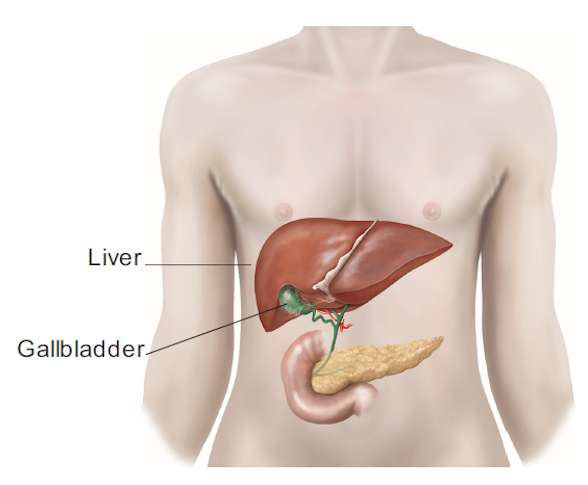
\includegraphics[width=\linewidth]{figs/gallbladder.png}
		\caption{}
		\label{fig:gb_whole}
	\end{subfigure}
	%
	\begin{subfigure}[b]{0.32\linewidth}
	\centering
	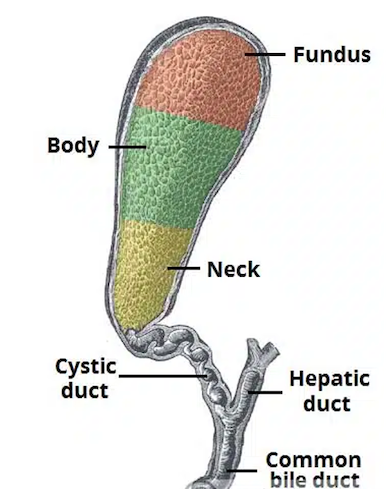
\includegraphics[width=\linewidth]{figs/gb_anatomy.png}
		\caption{}
		\label{fig:gb_anatomy}
	\end{subfigure}
	%
	\caption[Anatomy of Gallbladder in the human body]{(a) Anatomical positions of gallbladder and Liver in the human body. Image courtesy: Department of Health, Western Australia \cite{gb_image}. (b) The anatomical structure of the gallbladder including the three parts -- fundus, body, and neck.}
    \label{fig:gb}
\end{figure}

\par Inspired by the recent success of DNNs in medical imaging tasks, we systematically delve into the challenges involved in detecting Gallbladder Cancer (GBC) from diagnostic Ultrasound (USG). The Gallbladder (GB) is a hollow, pear-shaped and balloon-like gastrointestinal organ filled with bile juices and resides just under the liver. GB is found in the upper-right part of the abdomen. The anatomical structure of a GB consists of three parts -- (1) \emph{fundus}, the large rounded base that stores the bile, (2) \emph{body}, the tapered portion after fundus, and (3) \emph{neck}, the narrow and tapered area which joins with cystic duct. \cref{fig:gb} shows a pictorial overview of the anatomical position of the GB in the human body. Due to the contiguous tissues of GB with the liver, the malignancy in GB can quickly spread to the liver, adjacent organs, and lead to distant metastases (cancer spreading to distant organs). %The metastasis of gallbladder cancer can extend to neighboring tissues, organs, the entire abdominal cavity, or distant regions within the body. 
Despite previous efforts in the segmentation and detection of Gallbladder (GB) afflictions, such as detecting stones and polyps \cite{gbPolyp, gbPolyp2, gbAutomatic}, there is a noticeable gap in research concerning the application of DNNs for the detection of GBC. A search on Google Scholar with the keywords ``artificial intelligence'' and ``gallbladder cancer'' returned 204 articles between January 2015 and November 2021. In these, we did not find any published article on deep learning-based \gbc detection from \usg images. This gap emphasizes the need for further exploration into the utility of advanced neural network models in GBC detection, promising advancements in early diagnosis and improved patient outcomes. In the following sections, we discuss the implications and the motivation behind the study. 


\begin{figure}[t]
    \centering
    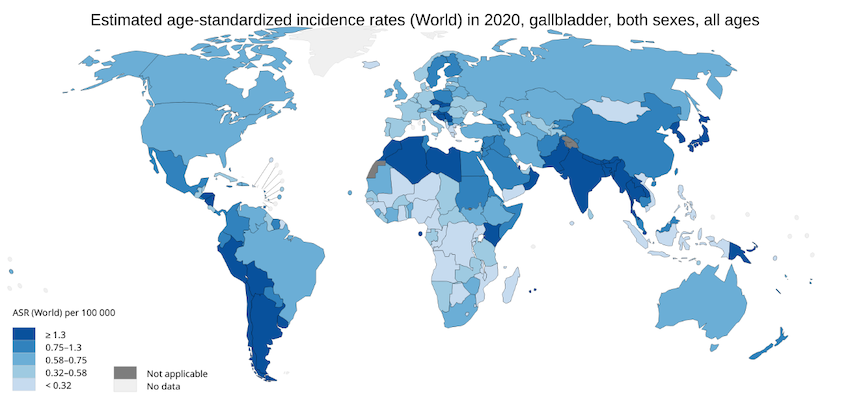
\includegraphics[width=0.8\linewidth]{figs/asr-map.png}
    \caption[The worldwide Age Standardized Incidence Rates (ASR) of GBC]{The worldwide Age Standardized Incidence Rates (ASR) of GBC. India sees a very high ASR, and is facing a significant risk of GBC. Image courtesy: GLOBOCAN \cite{bray2018global}.}
    \label{fig:asr_worldmap}
\end{figure}

\section{Gallbladder Cancer and its Risks}
%
\subsection{Gallbladder Cancer} 
% %
Gallbladder Cancer is an abnormal growth of cells that begins in the gallbladder. GBC is the most common biliary tract cancer and the fifth most common malignancy of the gastrointestinal tract \cite{HBSN4726}. According to GLOBOCAN 2020 data, GBC causes 84,695 deaths and 1,15,949 incidences every year worldwide \cite{armitage2014abeloff, bray2018global}. The disease is among the very few types of cancers which manifest a higher proportion of mortality than incidence \cite{bray2018global}. GBC has a very high mortality rate with 5-year survival rate of less than 5\% in patients with advanced disease.
The treatment involves surgically removing the GB and parts of surrounding regions from the hepatobiliary system when the malignancy is localized to GB and its wall. The surgical resection can also be followed with radiation or chemotherapy. For metastasized GBC, curative resection is infeasible, as the cancer has already spread to distant organs. GBC is overly deadly because it is rarely detected before an advanced and metastasized stage in most patients \cite{batra2005gallbladder, randi2006gallbladder}. 

%% Expand slightly

\subsection{Risks of GBC} 
% %
GBC is prevalent in China, India, and Latin America according to GLOBOCAN data \cite{bray2018global}. India, specifically, experiences a significant rise in Gallbladder Cancer (GBC). The incidence rate of GBC in India matches the globally highest rates. \cref{fig:asr_worldmap} shows the age-standardized incidence rates of GBC in different countries across the globe.
Furthermore, Indian patients contribute to more than 20\% of the annual mortality associated with Gallbladder Cancer (GBC). GBC also stands out as a leading cause of cancer-related deaths among Indian women \cite{randi2006gallbladder}. GBC is often detected at an advanced and metastasized stage for most patients, impeding curative resection and resulting in a dismal prognosis \cite{gupta2021locally, randi2006gallbladder}. 
%In fact, medical practitioners discover GBC by chance after a GB surgery in most cases. 
In the USA, only about 1 in every 5 cases of GBC are identified in an early stage \cite{howlader2017seer}. Although, early diagnosis provides an excellent chance to combat the disease by surgical removal, such timely diagnosis, unfortunately, is rare. The overall mean survival rate for patients with advanced GBC is six months, with a 5-year survival rate of 5\% \cite{levy2001gallbladder}. The median survival of patients with suspected GBC is 9.2 months, and 26.5 months for patients with incidental diagnosis \cite{wullstein2002complications}. Although GBC is relatively rare, its high mortality rate signifies the criticality of early diagnosis to improve the survival statistics of the deadly disease.  

\section{Motivation of the Study}
%
Early diagnosis and timely resection play a critical role in improving the survival rate of GBC. Studies indicate that the 5-year survival rate could be enhanced to 44\% with prompt medical interventions \cite{chen2016long}. USG is the most commonly used non-invasive diagnostic imaging method due to its non-ionizing radiation, portability, low cost, and widespread availability \cite{klibanov2015ultrasound}. Especially in India, Computed Tomography (CT) and Magnetic Resonance Imaging (MRI) are primarily accessible in tertiary care hospitals in big cities, and cost about ten times more than USG. Further, CT uses multiple X-ray images obtained from various angles to generate detailed cross-sectional images of the internal structures within the body, and thus expose the patients to X-ray radiation. USG is usually the de facto choice of diagnostic modality in low-resource settings, and serves as the primary imaging test for assessing GB diseases and is often the sole diagnostic tool for patients with suspected GB ailments. If no malignancy is suspected during the initial screening, further testing is usually not conducted, allowing GBC to progress silently. Surgical removal of GBC becomes infeasible at advanced stages.

\par Timely detection of GBC is crucial for enabling patients to undergo surgical and therapeutic interventions, ultimately improving the prognosis of the disease. Given that USG is the predominant diagnostic imaging modality for abdominal ailments, enhancing its ability to detect GBC would facilitate early diagnosis and contribute to improving survival statistics. Detecting signs of GBC through USG would provide healthcare professionals with a valuable tool for prompt intervention and treatment planning. The motivation of this work is leveraging the accessibility and widespread use of USG to enhance its effectiveness in identifying GBC (including accidental detections), thus positively impacting patient outcomes and survival rates.  

\section{Challenges of using Ultrasound}
%
Ultrasound (USG) operates by emitting high-frequency sound waves, typically in the range of 2--20 megahertz (MHz), from a transducer probe into the body. These sound waves travel through the body and bounce back (echo) when they encounter tissue boundaries or organs with different densities. The returning echoes are then detected by the transducer and converted into electrical signals, which are processed by a computer to generate real-time images of the internal structures. By analyzing the strength and timing of these echoes, ultrasound technology can create detailed images of organs, tissues, and blood flow without using ionizing radiation, making it a safe and non-invasive imaging modality. \cref{fig:usg_sample} shows USG images of the gallbladder. 
In \Cref{chap:usg} we provide more details on ultrasound imaging, the noise and artifacts inherent to ultrasound, and the relevant terminologies.


\begin{figure}[t]
    \centering
    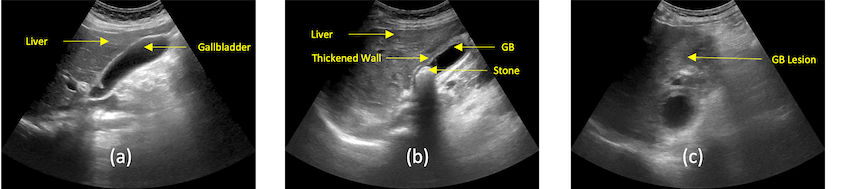
\includegraphics[width=0.95\linewidth]{figs/usg_sample.png}
    \caption[Ultrasound image samples]{USG image samples of the gallbladder (GB). (a) A normal GB along with the adjacent liver. (b) A GB with benign wall thickening and stone. (c) Malignant lesion at the GB.}
    \label{fig:usg_sample}
\end{figure}


Although USG is the primary diagnostic tool for assessing GB diseases, identifying the malignancy in routine USG remains a formidable challenge due to factors such as similar visual appearance with benign diseases, or confounding medical conditions (refer to \cref{sec:clinical}). Expert radiologists, even with years of experience, struggle to achieve more than 70\% sensitivity in GBC detection, indicating the need for more robust diagnostic methodologies.  Furthermore, the application of DNNs to analyze USG images faces significant hurdles, primarily stemming from the unique characteristics of USG imaging. USG images suffer from low quality due to noise, artifacts like shadows, and spurious textures, which can bias DNN classifiers and compromise detection accuracy. The handheld nature of ultrasound sensors introduces operator-specific visual variations across radiologists and medical centers, further complicating GBC detection. Further, malignant GB often presents irregular anatomy and low inter-class variability, making it challenging to distinguish from benign conditions. Moreover, the absence of well-annotated datasets poses a significant challenge for developing and training accurate DNN models for GBC detection, hindering progress in the field. We provide a detailed discussion about  challenges of using USG for GBC detection along with visual examples in \Cref{sec:challenges}. 


\section{Key Research Objectives}
%
The key research objectives of this thesis are as following:
\begin{itemize}
    \item Address the challenges posed by Ultrasound images, including noise, shadow, and spurious textures in detecting GBC and enhance the accuracy of GBC predictions by DNN models. 
    %
    \item Investigate techniques for learning from limited supervised data, particularly considering the scarcity of specialized annotations for medical data. Explore methods to leverage unlabelled or weakly labelled data for superior performance in GBC detection.
    %
    \item Explore methods to incorporate interpretability into model decision-making processes. Aim for models that provide insights into how predictions are reached, fostering better compatibility for clinical usage.
    %
    \item Assess the effectiveness of using Ultrasound video data directly for identifying GBC. Video-based detectors also eliminate the necessity for radiologists to select frames for GBC detection manually, reducing the effect of operator variability. 
    %
    \item Collect and curate annotated dataset in the form of both ultrasound images and videos to benefit the community. 
\end{itemize}



\section{Organization of Subsequent Chapters}
%
The thesis is organized into the following subsequent chapters:
    %\item \underline{Chapter I}: Introduction, providing a comprehensive overview of the research endeavor. The chapter outlines the problem statement, the motivation behind the study, the challenges, and the key research objectives that set the stage for subsequent chapters. 

\mypara{\Cref{chap:usg}} We briefly discuss the fundamentals of the Ultrasound imaging modality, and the issues and challenges associated with developing computer assisted methods for diagnosis of GBC from USG.  

\mypara{\Cref{chap:data}} In this chapter, we focus on the data used in this study and discuss the acquisition, curation, annotation, and statistics related to the data. 

\mypara{\Cref{chap:gbcnet}} We address the challenges associated with Ultrasound imaging, such as noise and artifacts, and provide the details of developing an accurate Gallbladder Cancer (GBC) detection model. An innovative classification model and a novel smoothing-based curriculum were the key technical contributions towards this end.
    
%\mypara{\Cref{chap:limited}} This chapter is centered on the issue of learning from limited supervised data, and investigates two distinct strategies -- (1) leverage unlabelled video data for achieving superior performance in downstream GBC detection, and (2) use weak image-level labels instead of the dense bounding box labels to train a GBC detector.

\mypara{\Cref{chap:limited}} This chapter is centered on the issue of learning from limited supervised data, and discusses how to leverage unlabelled video data for achieving superior performance in downstream GBC detection.

\mypara{\Cref{chap:wsod}} In this chapter, we present another alternative approach to learning from limited supervised data. We use weak image-level labels instead of the dense bounding box labels to train a GBC detector.

\mypara{\Cref{chap:radformer}} We investigate the development of explainable solutions for GBC detection in this chapter. The chapter critically analyzes interpretability in the context of model outputs, contributing to the broader understanding of decision-making processes.

\mypara{\Cref{chap:focusmae}} This chapter introduces and elucidates comprehensive video-based detection techniques. It explores the advantages and challenges of transitioning from images to video-based detection methods.

\mypara{\Cref{chap:conclusion}} The chapter serves as a conclusion, notes the limitations, and assesses the current and future scope of the work. We identify the potential avenues for further exploration and development and provide a roadmap for future advancements.


\chapter{Ultrasound and its Challenges in GBC Detection}
\label{chap:usg}
%
Ultrasound (USG), a non-invasive medical imaging technique, employs high-frequency sound waves to create real-time visualizations of internal body structures. 
%One commonly used mode is B-mode, or brightness mode, which produces two-dimensional images by interpreting the echoes of sound waves bouncing off tissues. B-mode ultrasound is invaluable for assessing organ structure and detecting abnormalities. 
Unlike X-rays, USG does not involve the use of ionizing radiation, which makes it safe for a wide range of patients. In this chapter, we provide a concise overview of USG fundamentals, followed by an exploration of the unique challenges encountered in automated GBC detection using USG. By delving into these intricacies, readers will gain a deeper understanding of the problem.
%we briefly discuss the basics of USG, and then describe the challenges posed by USG in automated GBC detection, providing the reader the necessary details for better understanding.

\section{Basics of Ultrasound}
%
\subsection{Ultrasound Physics}
Sound is a series of pressure waves that propagate through a compressible medium. A single \emph{cycle} of a sound wave encompasses a complete positive and negative pressure change. The \emph{wavelength} is defined as the distance covered during one complete cycle. The \emph{frequency} of the wave is measured in cycles per second, denoted as Hertz (Hz). The strength or the level of the pressure is called \emph{amplitude}. The audible range of sound for humans is 20 Hz to 20 kHz. Ultrasound refers to sound waves with frequencies higher than 20 kHz. In diagnostic ultrasound, frequencies between 1--20 MHz are commonly used.

Ultrasound wave production and interpretation rely on the `pulse-echo principle.' The process begins with the piezoelectric crystal within the transducer, acting as the source of ultrasound waves. This crystal has the capability to convert electrical current into mechanical pressure waves (ultrasound waves) and vice versa. Following the generation of the ultrasound wave, the crystal shifts from `sending' to `listening' mode, anticipating the return of ultrasound echoes. Notably, transducers spend almost all their time in the `listening' mode. The ultrasound waves can move through the tissues in both longitudinal and transverse directions. 
The sending and receiving cycle repeats a few million times per second, forming the foundation for creating images on the ultrasound monitor. The resulting images are contingent on the direction, timing, and amplitude of the returning waves.
Understanding the relationship between ultrasound frequency and image resolution is pivotal in selecting the appropriate probes and frequencies. Lower frequencies can penetrate deeper into tissue but provide poorer resolution for fine detail. Conversely, higher frequency ultrasound offers more detailed images with superior resolution but sacrifices depth penetration. This nuanced understanding is crucial for optimizing image quality and extracting meaningful diagnostic information.

\subsection{Common Modes of USG}
%
%\mypara{A-mode}
%
%In the amplitude mode (A-mode), the recording process captures the amplitude of the transducer voltage as a function to the round-trip travel time of an ultrasound pulse. A-mode operates by transmitting a single pulse through the body, with the pulse scattering back to the same transducer element. The recorded voltage amplitudes show a linear correlation to acoustic pressure amplitudes.

\mypara{B-mode}
%
B-mode, also known as `brightness mode,' offers structural information by representing different shades of gray in a two-dimensional image. The brightness in this mode is determined by the amplitude of returning echoes. Different echogenicities (brightness) are described as follows:
\begin{itemize}
    \item \emph{Anechoic:} Complete or near absence of returning sound waves, resulting in a black area.
    \item \emph{Hypoechoic:} Structure has very few echoes and appears darker than surrounding tissue.
    \item \emph{Hyperechoic/ Echogenic:} Large amplitude of returning echoes makes the structure appear brighter than surrounding tissue.
\end{itemize}
We show a sample B-mode USG along with the different brightness regions in \cref{fig:d_mode}.

\begin{figure}[!t]
\centering
	\begin{subfigure}[b]{0.32\linewidth}
	\centering
	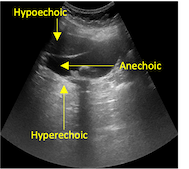
\includegraphics[width=\linewidth, height=8em]{figs/b_mode.png}
		\caption{}
		\label{fig:b_mode}
	\end{subfigure}
	%
	\begin{subfigure}[b]{0.32\linewidth}
	\centering
	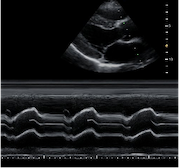
\includegraphics[width=\linewidth, height=8em]{figs/m_mode.png}
		\caption{}
		\label{fig:m_mode}
	\end{subfigure}
	%
        \begin{subfigure}[b]{0.32\linewidth}
	\centering
	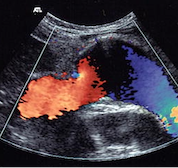
\includegraphics[width=\linewidth, height=8em]{figs/d_mode.png}
		\caption{}
		\label{fig:d_mode}
	\end{subfigure}
	\caption[Sample USG images from different modes]{Sample USG images from different modes. (a) B-mode, also highlights the anechoic, hypoechoic, and hyperechoic regions. (b) M-mode USG. (c) Doppler mode (color Doppler) USG.}
    \label{fig:usg_modes}
\end{figure}

\mypara{M-mode}
%
In motion mode, successive pulses are emitted. The backscattered signal is then converted into lines of bright pixels, where the brightness linearly correlates to backscattered voltage amplitudes. Each subsequent line is plotted adjacent to the previous one, producing an image resembling a B-mode image. This enables the visualization of movement in structures positioned along that line. A sample M-mode USG is shown in \cref{fig:m_mode}.

\mypara{Doppler mode}
%
Doppler mode involves analyzing the attributes of tissue motion and blood flow, including direction and speed. The core of this process relies on the `Doppler shift' phenomenon, which denotes the alteration in frequency between the transmitted and the returning sound wave. This technique is instrumental in capturing and interpreting the dynamic aspects of tissue motion and blood flow, providing valuable insights through various display modalities. \cref{fig:d_mode} shows a sample Doppler mode USG.
\begin{itemize}
    \item \emph{Color Doppler:} The direction and velocity of tissue motion and blood flow are color-coded and superimposed onto the corresponding B-mode image. 
    \item \emph{Power Doppler:} Captures the amplitudes of the returning frequency shifts onto the corresponding B-mode image. Typically used during vascular emrgencies with low flow state.
    \item \emph{Spectral Doppler:}  The spectrum of the Doppler frequencies returning to the transducer are Fourier transformed, and presented in a continuous and pulse-wave form.
\end{itemize}

\begin{figure}[!t]
    \centering
    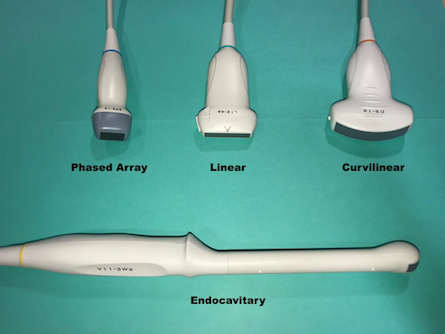
\includegraphics[width=0.5\linewidth]{figs/usg_probes.png}
    \caption[Common USG probes]{Four common types of probes used in diagnostic ultrasound imaging. Image courtesy: American College of Emergency Physicians \cite{acep}.}
    \label{fig:usg_probes}
\end{figure}

\subsection{Types of Probes}
%
Transducers or probes are comprised of three main components: the active element, which is typically a piezoelectric crystal, a damping material, and a matching layer. The arrangement of the active element can take various forms, resulting in a variety of probe configurations. Following are few of the most commonly used probe types,
\begin{enumerate}
    \item \textbf{Curvilinear (Curved Array):} This type of probe has a large curved footprint. The curved array probes produce images with shape resembling to the sector of a circle. These probes operate on low frequency, and are primarily employed for transabdominal ultrasound. 
    %
    \item \textbf{Phased Array:} This transducer produces a sector-shaped image with a smaller footprint, making it ideal for use between ribs. It operates at a low frequency and is primarily employed in cardiac and transabdominal ultrasound.
    %
    \item \textbf{Linear:} This transducer generates a rectangular image with a straight, flat footprint and is characterized by a high frequency. Its primary applications include vascular ultrasound, procedural guidance, and the assessment of superficial soft tissue structures.
    %
    \item \textbf{Endocavitary:} This transducer has a small curved footprint, and operates at a medium frequency. These are primarily used for endovaginal or intraoral ultrasound.
\end{enumerate}
\cref{fig:usg_probes} shows the curvilinear and the other commonly used probes.

\subsection{Body Planes}
%
\begin{figure}[!ht]
    \centering
    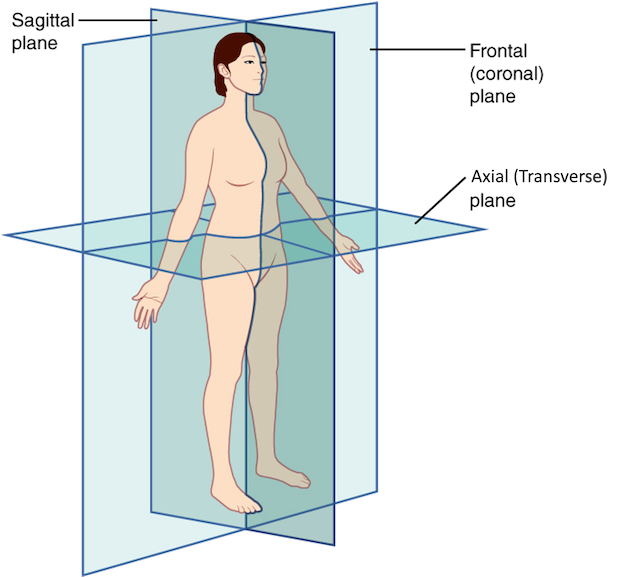
\includegraphics[width=0.5\linewidth]{figs/body_planes.png}
    \caption[Different body planes for radiological scanning]{The three different body planes relevant for scanning in radiology. Image courtesy: Wikipedia \cite{body_plane}.}
    \label{fig:body_plane}
\end{figure}
The \textbf{sagittal plane} is oriented perpendicular to the ground, distinguishing the left from the right, when an individual is in a \emph{supine position}. In supine position, a person lies on their back with the face and torso facing upwards.

The \textbf{axial plane}, also called the \textbf{transverse plane} or cross-sectional plane, is positioned perpendicular to the ground when the patient is in a supine posture. It differentiates the superior from the inferior or the head from the feet.

In the supine position, the \textbf{frontal plane}, also known as the coronal plane, aligns parallel to the ground, distinguishing the anterior from the posterior or the front from the back.

The illustration in \cref{fig:body_plane} depicts the three distinct body planes that are pertinent for scanning in radiology.

In addition to the three standard scanning planes, an \textbf{oblique plane} may also be used by the radiologist. As the name suggests, oblique plane is any plane which is not parallel or not in right angle to any of sagittal, axial, and frontal planes.

% \subsection{Probe Movements}
% %
% In ultrasound imaging, various movements of the probe are employed for effective examination \cite{bahner2016language}:

% \begin{itemize}
 
%     \item \textbf{Slide:} This involves moving the probe in the long axis along the surface of the body. The probe remains perpendicular to the target.

%     \item \textbf{Sweep:} This entails moving the probe in the short axis along the surface of the body. Similar to sliding, the probe remains perpendicular to the target.

%     \item \textbf{Rock:} In this movement, the probe travels along its long axis without changing the point of contact between the probe and the surface of the body.

%     \item \textbf{Fan:} The probe moves along its short axis without changing the point of contact between the probe and the surface of the body.

%     \item \textbf{Pressure:} This movement involves pushing the probe into the surface of the body. The footprint maintains contact with the surface, and the probe remains perpendicular to the target.

%     \item \textbf{Rotate:} The probe is rotated either clockwise or counterclockwise. The footprint maintains contact with the surface of the body, and the probe remains perpendicular to the target.
% \end{itemize}

\begin{figure}[!t]
\centering
    \begin{subfigure}[b]{0.32\linewidth}
    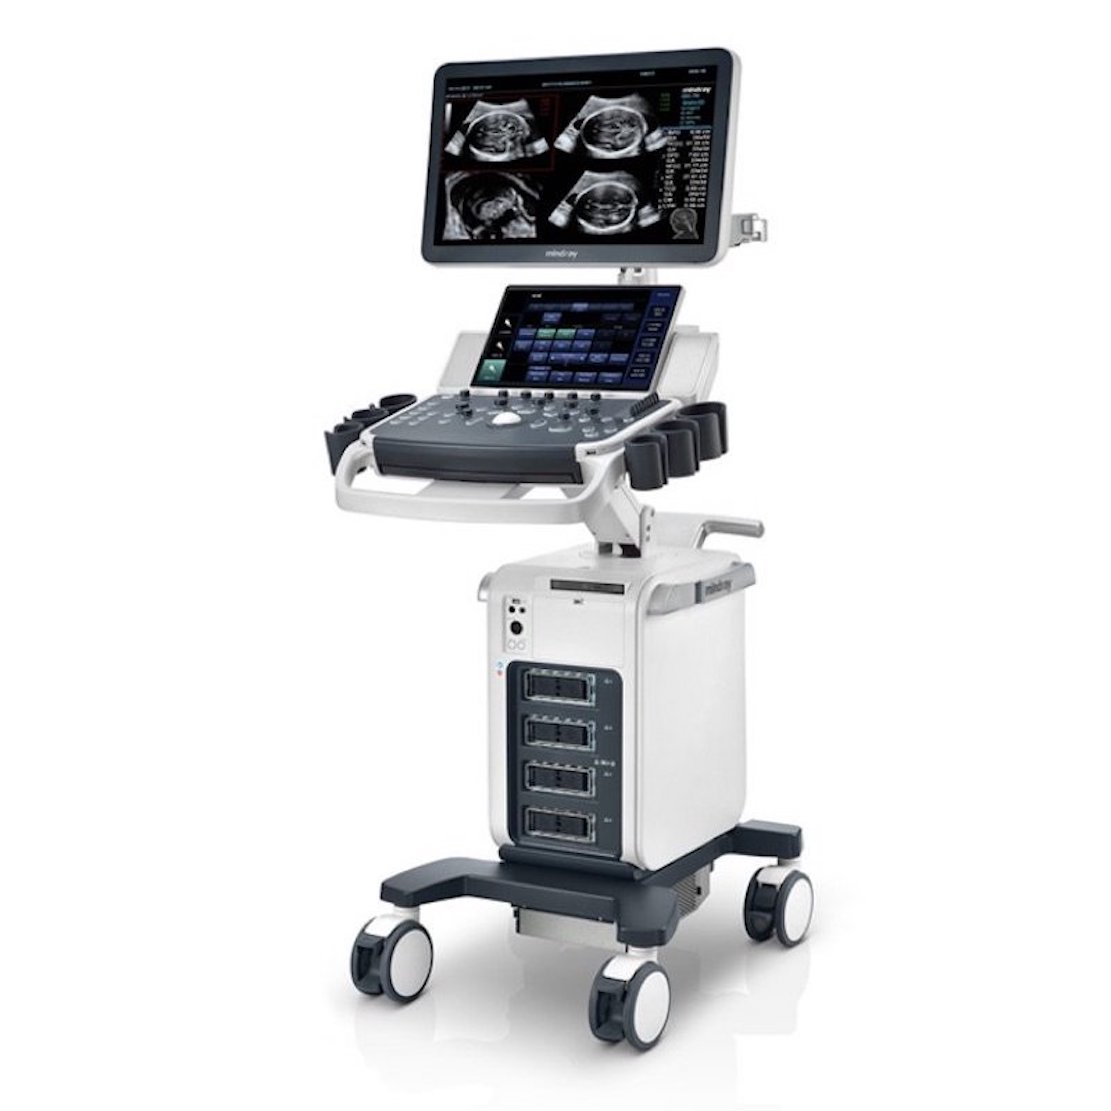
\includegraphics[width=\linewidth, height=8em]{figs/usg_machine.jpg}
    \caption{}
    \label{fig:usg_machine}
    \end{subfigure}
    %
    \begin{subfigure}[b]{0.24\linewidth}	
    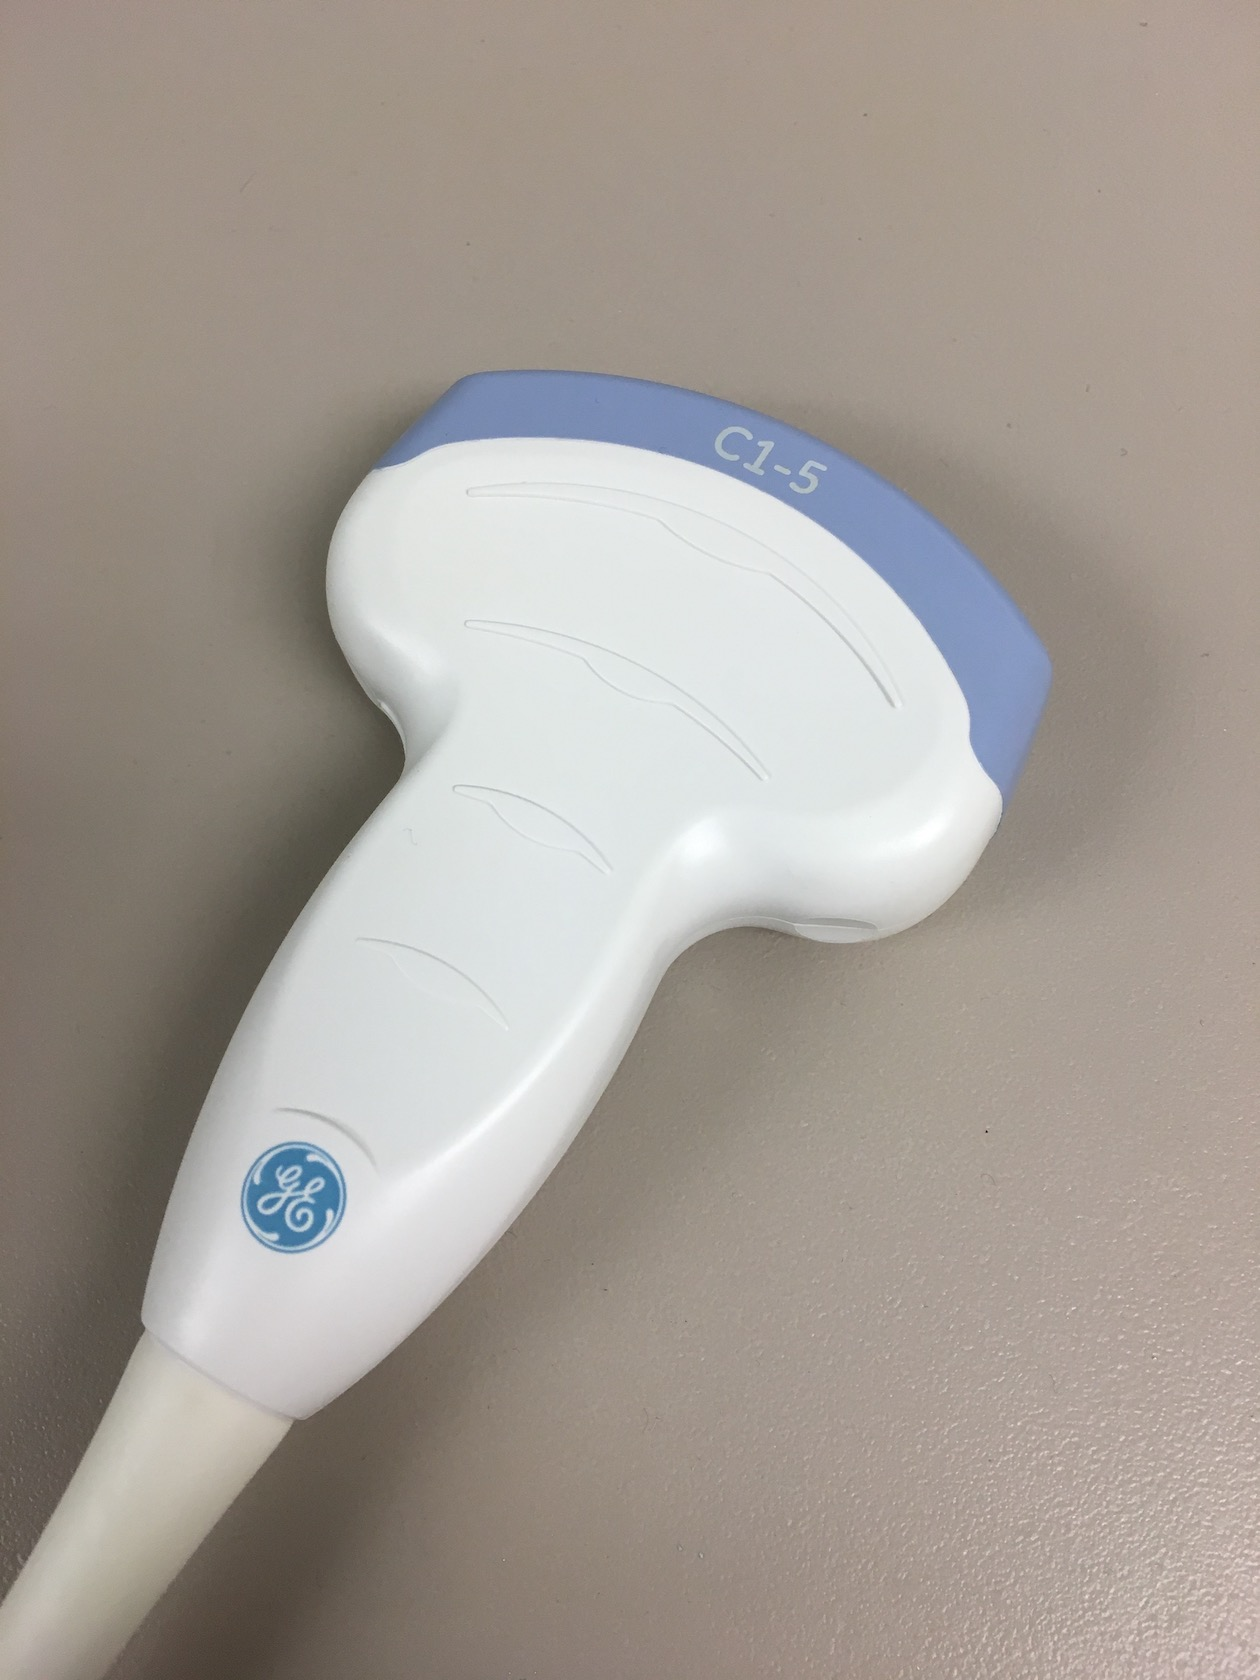
\includegraphics[width=\linewidth, height=8em]{figs/transducer.jpg}
    \caption{}
    \label{fig:usg_probe}
    \end{subfigure}
    %
    \begin{subfigure}[b]{0.32\linewidth}	
    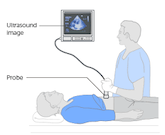
\includegraphics[width=\linewidth, height=8em]{figs/usg_overall.png}
    \caption{}
    \label{fig:usg_diag}
    \end{subfigure}
    \caption[Ultrasound machine, probe, and schematic diagram of abdominal USG]{(a) An USG machine with the display on top, control panel in the middle, and the computing engine on the base. (b) A curvilinear transducer (also called probe or sensor) commonly used for abdominal USG. (c) Schematic diagram of the USG procedure. Image courtesy: Cancer UK \cite{usg_diag}.}
    \label{fig:sample_usg}
\end{figure}

\section{Brief Description of Abdominal USG}
%
Abdominal USG focuses on scanning the organs within the abdominal cavity. It provides detailed views of the liver, kidneys, gallbladder, pancreas, and other abdominal structures, aiding in diagnosing conditions such as liver disease, kidney stones, or gallbladder ailments.

\par The USG scanning procedure involves applying a gel to the patient's skin to facilitate sound wave transmission and then using a transducer to emit and receive the waves. The resulting images guide healthcare professionals in making accurate diagnoses without the need for invasive procedures. Usually a handheld curved array probe is used for abdominal USG. The probe serves as both an emitter and receiver of sound waves. When the waves encounter different tissue densities, they reflect back to the transducer at varying speeds, forming a detailed image on the monitor. Radiologists strategically position the transducer on the patient's skin, manipulating its orientation and depth to capture comprehensive views of the targeted area. \cref{fig:usg_diag} shows a schematic diagram of the scanning process and the transducer probe.
Overall, USG combines sophisticated technology with skilled operator expertise to provide detailed, real-time images that aid in the affordable and safe diagnosis and monitoring of various medical conditions.

\section{Brief Specification of Our Data}
%
We have collected patient data from the Radiology department of a tertiary care apex hospital in Northern India. Patients were scanned using a Logiq S8 (GE Healthcare) machine with a low-frequency curvilinear probe (C1-5-D) operating at a frequency of 1-5 MHz in B-mode ultrasound. We have curated image data for 218 patients (1155 images), and video data for 73 patients (91 videos). We obtained written patient consent, and anonymized the data to protect patient privacy as per Ethics committee guidelines. Ultrasound scans were captured from different views and scanning planes to ensure adequate visualization of the pathology. 
In \Cref{chap:data} we provide more details regarding the dataset collection, annotation, and data statistics. In the following sections in this chapter, we outline the noise and artifacts in abdominal USG, the challenges of detecting GBC from USG, and also the specific issues pertaining to our data.

%\subsection{Applications of USG}
%
\section{Noise and Artifacts in Abdominal Ultrasound}
\label{sec:artifact_in_usg}

\begin{figure}[!t]
\centering
    % \begin{subfigure}[b]{0.23\linewidth}
    % 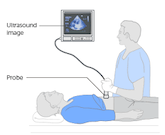
\includegraphics[width=\linewidth, height=6em]{figs/usg_overall.png}
    % \caption{}
    % \label{fig:usg_diag}
    % \end{subfigure}
	\begin{subfigure}[b]{0.24\linewidth}
	\centering
	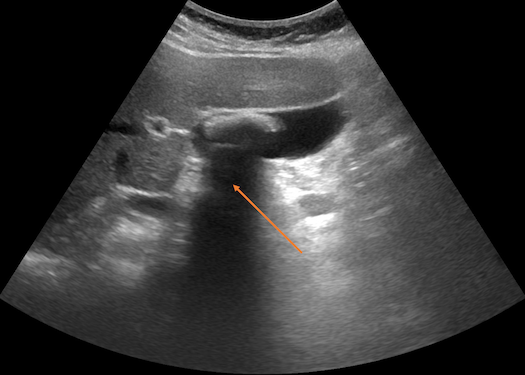
\includegraphics[width=\linewidth, height=7em]{figs/shadow.png}
		\caption{}
		\label{fig:usg_shadow}
	\end{subfigure}
	%
	\begin{subfigure}[b]{0.24\linewidth}
	\centering
	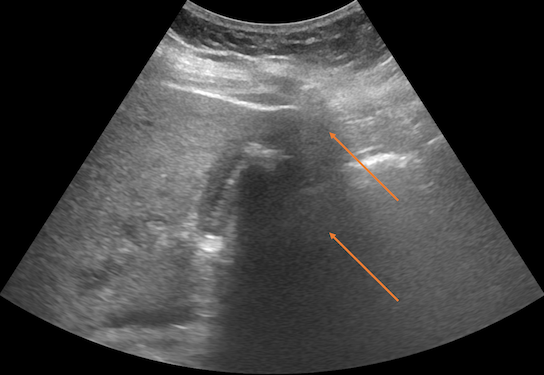
\includegraphics[width=\linewidth, height=7em]{figs/speckle.png}
		\caption{}
		\label{fig:usg_speckle}
	\end{subfigure}
	%
        \begin{subfigure}[b]{0.24\linewidth}
	\centering
	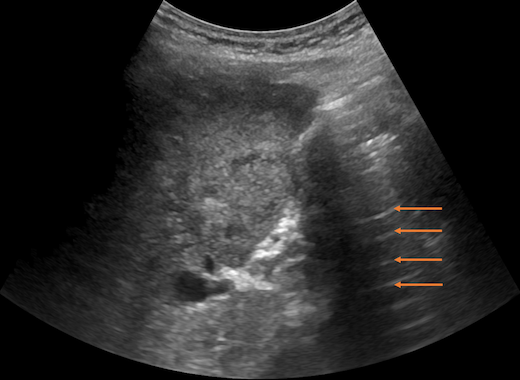
\includegraphics[width=\linewidth, height=7em]{figs/reverb.png}
		\caption{}
		\label{fig:usg_reverb}
	\end{subfigure}
    %
        \begin{subfigure}[b]{0.24\linewidth}
	\centering
	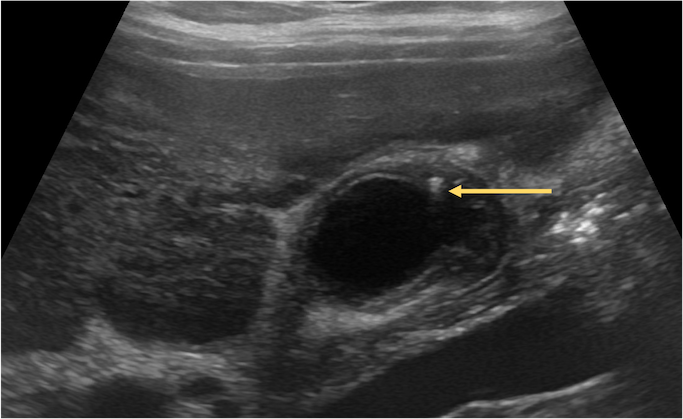
\includegraphics[width=\linewidth, height=7em]{figs/comet_tail.png}
		\caption{}
		\label{fig:usg_comet}
	\end{subfigure}
	\caption[Visualization of common artifacts present in our data]{Visualization of common artifacts present in our ultrasound dataset. (a) Ultrasound image sample showing the acoustic shadow artifacts caused by solid objects such as gallbladder stones. (b) Example of the speckle noise present in USG. (c) Reverberation artifact in ultrasound images. (d) Comet tail artifact in gallbladder. }
    \label{fig:sample_artifact_usg}
\end{figure}

%
In abdominal ultrasound imaging, various types of noise and artifacts can affect the quality and accuracy of the images produced. These artifacts may arise from factors such as equipment limitations, patient anatomy, or the interaction of sound waves with tissues. Understanding these artifacts is crucial for radiologists in interpreting ultrasound results. Such artifacts also influence the outcome of the DNN models. We briefly highlight some common types of artifacts found in ultrasound imaging, especially the ones our data manifested in this section. 

\mypara{Acoustic Shadows} This artifact occurs when sound waves encounter a strongly reflective or absorptive structure, leading to a shadow on the image. For example, bones or gallstones can cause acoustic shadowing, making it challenging to visualize structures behind them. \cref{fig:usg_shadow} shows a sample of the acoustic shadowing caused by a gallbladder stone. In our data, the acoustic shadows played a significant role in degrading the performance of popular off-the-shelf DNN models.
    
\mypara{Speckle Noise} A Speckle is a granular pattern that can appear on ultrasound images. It is a form of noise caused by interference patterns in the ultrasound beam. Speckle noise in inherent to ultrasound imaging, and is illustrated in \cref{fig:usg_speckle}. Our data samples also contained speckled noise. Advanced image processing techniques involving smoothing are usually employed to reduce the impact of speckle noise \cite{despeckle}. 
    
\mypara{Reverberation} Reverberation artifacts happen when sound waves bounce back and forth between two strong reflectors, creating multiple equally spaced lines on the image. This can create false echoes and distort the interpretation of structures. In our data, reverberation was another common artifact. \cref{fig:usg_reverb} presents an example of the reverberation artifacts from our dataset, highlighted with arrows. 
    
\mypara{Comet Tail Artifact} Similar to reverberation, a comet tail artifact is a dense line extending from a highly reflective structure. It is often seen behind gas bubbles or calcifications and may obscure the details of nearby structures. Some samples of our data demonstrated comet tail artifact. One such sample is shown in \cref{fig:usg_comet}. However, comet tail artifact is usually associated with benign GB pathology such as adenomyomatosis \cite{oh2019comet}, and is helpful for radiologists. 
    
%\mypara{Anisotropy} When ultrasound waves encounter a fibrillar structure, like a tendon or ligament, the fibrils can redirect a significant portion of the incoming sound beam away from the transducer. In such instances, the transducer does not capture the returning echo, leading it to interpret the insonated area as hypoechoic (darker than surrounding tissues). This happens because the majority of the reflected sound waves move away from the transducer, causing it to infer a reduced echogenicity (brightness of an area) in the imaged region. Anisotropy is usually manifested in Musculoskeletal ultrasound. 
    %
    %\item \mypara{Slice Thickness} This artifact occurs when the ultrasound beam has a finite thickness, causing structures to appear larger than they actually are. It can affect the accuracy of measurements and spatial resolution.
%

Understanding and recognizing these issues is essential to differentiate between genuine anatomical features and artifacts, ensuring accurate diagnosis and interpretation of ultrasound images. 

\section{Major Challenges}
\label{sec:challenges}
%% Expand the subsections -- some more elaboration
%
While identifying benign afflictions, such as stones, polyps, or GB wall thickening in routine USG is straightforward, accurate characterization and GBC detection is challenging for the radiologists \cite{gb-rads-paper, gupta2020imaging}. Our findings show that even the expert radiologists with 10 and 2 years of experience in abdominal radiology could only attain a sensitivity of about 70\% while detecting GBC from USG. In this section, we first describe the clinical challenges faced by radiologists, and then highlight the significant obstacles arising from noise, artifacts, and viewpoint variations in USG, which we encountered while applying DNN models to analyze USG images in this work. We have tackled issues including noise and artifacts such as acoustic shadows and bias to echogenic textures, small sized pathological regions, variation in appearance due to non-regular anatomy and operator bias, and low volume of data.  %These challenges and the solutions to remediate them are discussed in the subsequent chapters.

\begin{figure}[t]
    \centering
    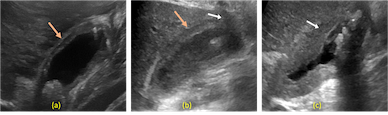
\includegraphics[width=0.8\linewidth, height=7em]{figs/clinical.png}
    \caption[Appearances of benign and malignant wall thickening]{(a) Shows a benign wall thickening with typical eco-layering (orange arrow). (b) Presents the wall thickening in a pathologically proven malignant GB. Notice the layered appearance (marked with the orange arrow) in this malignant thickening. Further, the thickening appears diffuse and symmetric, which is typically observed in benign cases. (c) Another pathologically proven case of GBC. Note that the wall thickening is more pronounced and irregular unlike the benign thickening.}
    \label{fig:clinical}
\end{figure}

\subsection{Challenges in Clinical Characterization of GB Wall Thickening}
\label{sec:clinical}
%
Clinical characterization of benign versus malignant GB wall thickening is challenging for even the experienced Radiologists due to multiple overlapping imaging features. Although GBC typically manifests asymmetric and irregular wall thickening, early stages of the disease may also manifest smooth and symmetric wall thickening, which is typical for benign conditions \cite{gupta2020imaging}. Additionally, as highlighted in \cref{fig:clinical}, traditional signs of benign thickening, like echo-layering (layered appearance) of the gallbladder wall, may also manifest in malignant cases, leading to diagnostic uncertainty. Furthermore, gallbladder wall thickening can occur in various conditions beyond GBC, such as acute cholecystitis, hepatitis, renal failure, pancreatitis, and Rokitansky-Aschoff sinuses \cite{gbc-lancet, gbc-xgc, gupta2020imaging}. The presence of these confounding factors can obscure the distinction between benign and malignant causes of wall thickening.
%the presence of various confounding factors, including systemic illnesses, can obscure the distinction between benign and malignant causes. As diagnostic criteria evolve, features once considered specific to benign conditions may be found in malignant cases as well, complicating interpretation. 
Ultimately, definitive diagnosis often requires histopathological evaluation to differentiate between benign and malignant pathologies conclusively, as radiologists often face difficulty in detecting GBC through non-invasive methods such as ultrasound. DNN methods can bridge this gap in non-invasive detection of GBC.

\begin{figure}[t]
    \centering
    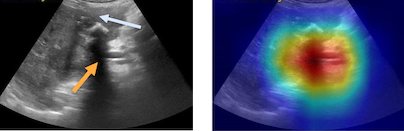
\includegraphics[width=0.8\linewidth]{figs/shadow_bias.png}
    \caption[Visualization of issues arising from artifacts such as acoustic shadow]{The black shadow (highlighted by the orange colored arrow) in the center of the left side image has visual similarities with the appearance of a normal \gb. The blue colored arrow shows the malignant region in the image. On the right side, we show the Grad-CAM \cite{gradcam} visual of a fine-tuned ResNet-50 \cite{resnet} model to visualize the salient region localized by the model. Clearly, the model is not accurately picking up the malignant regions, and is getting biased by the shadow region.}
    \label{fig:shadow_bias}
\end{figure}

\begin{figure}[t]
    \centering
    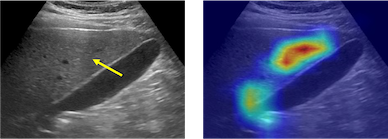
\includegraphics[width=0.8\linewidth, height=10em]{figs/texture_bias.png}
    \caption[Textures of liver tissues leading to incorrect GBC predictions]{The echogenicity of liver tissues resemble to gallbladder lesions/ masses. The adjacent liver tissue textures can bias the DNNs and lead to incorrectly predicting a normal gallbladder to be malignant. Liver is shown with yellow arrow in left image. On the right, we see from the Grad-CAM visual that Resnet-50 identifies the liver tissues as salient regions, and incorrectly predicts malignancy.}
    \label{fig:texture_bias}
\end{figure}

\begin{figure}[!ht]
    \centering
    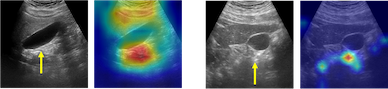
\includegraphics[width=0.8\linewidth]{figs/bright.png}
    \caption[Visualization of DNN models getting biased by hyperechoic regions]{The hyperechoic regions (highlighted by the yellow arrows) may bias the DNNs, and appear more distinctive over the GB regions to the networks. We show the Grad-CAM visual of a fine-tuned ResNet-50 model to identify the salient region localized by the model. The model is not accurately localizing the normal GB in these images, and instead focus on the bright regions.}
    \label{fig:hyperechoic_bias}
\end{figure}

\subsection{Low Image Quality -- Noise and Artifacts}
\label{sec:usg_artifact_issue}
%
% GBC detection from USG faces major challenges from low image quality, marked by noise, artifacts like shadows, and spurious textures. Unlike CT or MRI, USG suffers from low image quality arising from the noise and artifacts, as discussed previously in \cref{sec:artifact_in_usg}. Artifacts such as the shadows often show the visual traits of a non-malignant GB region, introducing bias to state-of-the-art DNN classifiers and resulting in suboptimal detection accuracy \cite{basu2022surpassing}. We present one such example in \cref{fig:shadow_bias}. The shadow region has a visual semblance with the appearance of the GB in ultrasound images. A finetuned Resnet-50 model identifies this region as a salient region, and results in incorrect prediction. 
% Additionally, The handheld nature of ultrasound sensors introduces operator-specific visual variations across radiologists and medical centers. These cause a large  The handheld nature of the sensor, and the operator-specific biases in view selection can result in radiologists selecting different frames from an USG scan (available in the form of a video) for assessment, introducing inter-observer variability. 

% Further, malignancy usually appears in a small part of the image, resulting in the low inter-class variability of the data. Also USG images are 2D slices of the 3D organs. The handheld nature of the probe causes large variation in different view points within the same patient, causing high intra-class variability. These issues make accurate prediction difficult for the DNN models. \cref{wsod_fig:variability_teaser} presents a depiction of the low inter-class and high intra-class variability.
Using DNNs to detect GBC from USG images presents formidable challenges arising from the inherent limitations in image quality. The USG modality, unlike CT or MRI, is susceptible to sensor artifacts, such as noise, shadows, and spurious textures. The low image quality arising from the sensor artifacts is a crucial factor complicating the accurate identification of malignant features in gallbladder regions, as discussed in \cref{sec:artifact_in_usg}. We further elaborate the specific challenges that we came across during the course of this work.

One notable challenge lies in artifacts like shadows or the anechoic regions, which often exhibit visual traits resembling non-malignant gallbladder regions. This introduces a bias to contemporary DNN classifiers, resulting in suboptimal detection accuracy \cite{basu2022surpassing}. A concrete example of this challenge is illustrated in \cref{fig:shadow_bias}, where a shadow region, sharing visual similarities with the gallbladder, is erroneously predicted as a salient region by a finetuned Resnet-50 model. 

The echogenic textures of the soft tissues of the organs such as liver often resemble the gallbladder lesions. Such textures appearing near the GB region can mislead a DNN model into falsely detecting malignancy. \cref{fig:texture_bias} demonstrates such an event of the model identifying the liver tissue as the salient region, and incorrectly predicting the sample to be malignant.

Additionally, standard DNNs may also get biased by the bright or hyperechoic regions, as these regions could appear distinctive to the networks. \cref{fig:hyperechoic_bias} shows an example of a Resnet-50 model focusing on the region with increased echogenicity. 



\subsection{Handheld Transducer -- Viewpoint and Operator Variability}
%
The handheld nature of ultrasound transducers (probes) adds another layer of complexity. It introduces operator-specific visual variations across different radiologists and medical centers, contributing to inter-observer variability. 
We further note that USG images provide 2D slices of 3D organs. Thus the angle of the transducer can significantly influence the appearance of the GB, and cause substantial variation in viewpoints within the same patient. Due to the change in the angle of insonation, some artifacts resembling the polypoidal mass can be observed in an otherwise normal gallbladder. \Cref{fig:angle_pseudo} presents an example of how changing the view from sagittal to axial leads to the pseudo-appearance of an artifact. 

\begin{figure}[t]
    \centering
    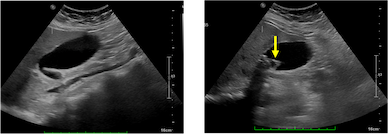
\includegraphics[width=0.6\linewidth, height=8em]{figs/angle_pseudo.png}
    \caption[Angle of transducer causing pseudo structures]{Sagittal (on left) and axial (on right) views of the gallbladder in a patient. On sagittal view, the GB wall is uniformly smooth and normal. The axial images gives a false appearance of the polypoidal mass arising from the gallbladder wall. This pseudo-appearance is due to the angle of insonation, and causes incorrect diagnosis.}
    \label{fig:angle_pseudo}
\end{figure}

\begin{figure}[!ht]
    \centering
    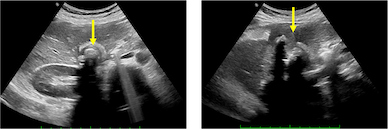
\includegraphics[width=0.6\linewidth, height=8em]{figs/oblique_thickening.png}
    \caption[Viewpoint variation leading to incorrect diagnosis]{True axial (on left) and Oblique axial (on right) views of the gallbladder in a patient with large gallstones. On true axial view, the GB wall characteristics are those of benign thickening. However, in the oblique view, the wall thickening appears to be infiltrating the adjacent liver, and leads to misclassification as malignant. }
    \label{fig:oblique_thickening}
\end{figure}
%\subsection{Angle of Transducer Leading to Viewpoint Variations}
%
%\subsection{Angle of Transducer Leading to Viewpoint Variations}
%
%We further note that USG images provide 2D slices of 3D organs. Thus the angle of the transducer can significantly influence the appearance of the GB, and cause substantial variation in viewpoints within the same patient. Due to the change in the angle of insonation, some artifacts resembling the polypoidal mass can be observed in an otherwise normal gallbladder. \Cref{fig:angle_pseudo} presents an example of how changing the view from sagittal to axial leads to the pseudo-appearance of an artifact. 

In another example in \cref{fig:oblique_thickening}, we show how the different probe axis leads to different interpretation for the same patient. The true axial image of the gallbladder shows benign wall thickening. However, in an oblique axial view, the mural (wall) thickening seems to be infiltrating the adjacent liver leading to incorrect diagnosis as malignant.

Further, different radiologists can select different representative frames/ views from an USG scan (available in the form of a video) for assessment, thus exacerbating the observer variability. 

\begin{figure}[t]
    \centering
    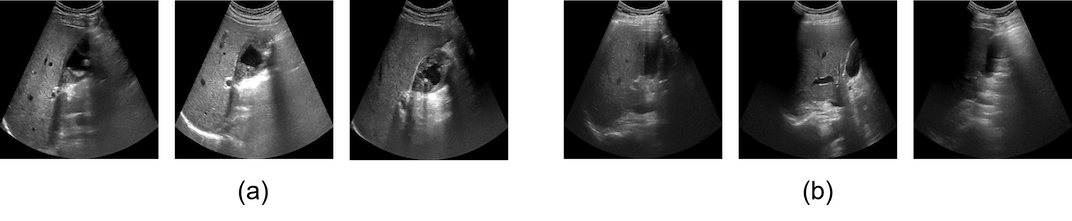
\includegraphics[width=0.9\linewidth]{figs/wsod/teaser.png}
    \caption[Low inter-class and high intra-class variability of GBC in USG data]{(a) Low inter-class variability. The first two GBs show benign wall thickening, and the third one shows malignant thickening. However, the appearance of the GB in all three images is very similar. (b) High intra-class variability. All three images have been scanned from the same patient, but due to the sensor's scanning plane, the appearances change drastically.}
    \label{wsod_fig:variability_teaser}
\end{figure}

\begin{figure}[t]
    \centering
    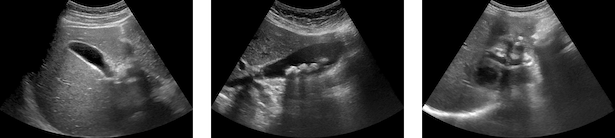
\includegraphics[width=\linewidth]{figs/non_reg_anatomy.png}
    \caption[Visualization of non-regular anatomy of the malignant gallbladders]{Normal, benign, and malignant \gb sample in \usg images, respectively (left to right). While normal or benign \gb have a regular, pear-shaped anatomy, a clear boundary is absent in the malignant \gb.}
    \label{fig:non_reg_anatomy}
\end{figure}


\subsection{Low Inter-Class and High Intra-Class Variability}
%
The manifestation of malignancy often occurs in a small part of the image, resulting in low inter-class variability, as most part of the images contain similar visual appearances. Also, as discussed earlier, the conflicting appearances in some of the benign and malignant wall thickening adds to the low inter-class variability. Simultaneously, USG images manifest significant variability in viewpoints for the same patient due to the handheld probe. This results in high intra-class variability, adding to the intricacies of accurate prediction for DNN models, as depicted in \cref{wsod_fig:variability_teaser}. The amalgamation of these challenges underscores the need for innovative solutions in GBC detection from USG images.

\begin{figure}[t]
    \centering
    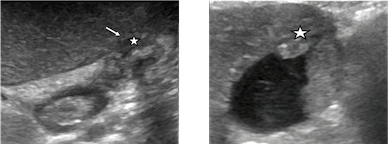
\includegraphics[width=0.8\linewidth]{figs/fasting.png}
    \caption[Effect of metabolic state on GB distension]{On left, the patient was in non-fasting state. On right, the patient was in fasting for 12 hours. Note the wall characteristics are much well appreciated in fasting state. Stars point to the focal thickening of the wall with adjacent liver infiltration. }
    \label{fig:fasting}
\end{figure}

\subsection{Non-regular Anatomy}
%
% Malignant GB usually exhibits non-regular anatomy, including a loss of interface with adjacent organs and irregular anatomical structure. \cref{fig:non_reg_anatomy} highlights the issue pictorially. The non-malignant GB in most cases demonstrate a clear anatomical pear-shaped structure. However, for malignant GBs, the entire GB is most cases is replaced by lesion or mass, making it difficult to even conclude the presence of a GB. 

The detection of gallbladder malignancy is further complicated by the non-regular anatomy typically associated with malignancy. Malignant gallbladders often showcase irregularities such as a loss of interface with adjacent organs and a distorted anatomical structure. \cref{fig:non_reg_anatomy} visually highlights this issue. In non-malignant cases, the GB typically exhibits a clear pear-shaped structure with distinct anatomical features. However, for malignant gallbladders, the entire gallbladder is frequently replaced by a lesion or mass, making it challenging to even identify the presence of a gallbladder in certain cases. Such non-regular anatomy further emphasizes the intricacies involved in distinguishing between malignant and non-malignant cases in USG images.

\subsection{Effect of the Metabolic State of the Patients}
%
If the patients are in fasting state, the gallbladder is well distended, and the abnormalities can be well detected. However, if the patient is not in fasting state, the contracted gallbladder adds to the difficulty of diagnosis. \Cref{fig:fasting} shows how acquiring the image samples after keeping the patient in 12-hour fasting helps in obtaining a better view of the gallbladder. Thus, it is important to obtain the data in the correct metabolic state to ensure the presence of adequate visual features in the captured images.

\subsection{Lack of Annotated Data}
%
%The absence of a well-annotated dataset poses another challenge for developing and training accurate DNN models for GBC detection, hindering progress in the field. Prior to our work, there was no public dataset with annotated USG images or videos for training the GBC detectors. 
The lack of a well-annotated dataset presents an additional hurdle in the development and training of accurate DNN models for GBC detection, impeding advancements in the field. Prior to our research, public datasets with annotated Ultrasound images or videos for training GBC detectors did not exist. The absence of comprehensive and annotated datasets significantly hampers the ability to train and optimize DNN models for the specific task of GBC detection, highlighting the need for dataset contributions and novel approaches involving training with a low volume of data in this domain.

\subsection{Challenges Addressed in this Work}
%
In this work, our developed techniques in Chapters 4--8 could solve the issues arising from the noises and artifacts such as acoustic shadows, bias to echogenic textures, small sized pathological regions, variation in appearance due to non-regular anatomy to a large extent in our data. To tackle the lack of annotated data, self-supervised representation learning has also been utilized. The issues related to operator and viewpoint variability largely affects the image-based GBC detectors. The use of video-based detectors could mitigate the effect of operator and viewpoint variability.

It is important to note that we have primarily addressed multiple issues of DNN-based malignant vs. benign GB  differentiation on single-center retrospective ultrasound data. Further, staging of malignancy, or differential diagnosis were not studied. A precise assessment of the methods in tackling acquisition shifts and their generalization performance requires more data from different centers, as single-center data only involves a few radiologists and a limited set of ultrasound apparatus. Due to the absence of publicly available data or other hospitals' data, we could not quantitatively assess the robustness and generalization performance for GBC detection, and noted it as a future research direction. However, it is important to note that the inherent issues such as noise, textures, and non-regular anatomy would remain constant for GBC ultrasound data from other centers. Additionally, we have demonstrated the generality and applicability of the developed methods on datasets for other diseases, such as breast cancer, COVID-19, and polyp detection, indicating the generalizability of the methods.

Furthermore, our data collection was from an apex tertiary care hospital in Northern India, which attends patients from different states, ethnicities, genders, and demographics. The patients are not localized to the region of the hospital, and far-off patients also visit for care. This ensures a high degree of patient variability in our data. Thus, we expect our techniques to perform robustly. Nonetheless, some performance drop is expected while applying the models on unseen data from other centers due to operator and equipment variability. %Especially image-based detection models tend to be more susceptible to acquisition shift arising from operator variability.

%In this work, we have primarily addressed multiple issues on single-center retrospective patient data. The use of techniques such as focused regions-of-interest, smoothing-based curriculum, multi-scale features, second order feature attention, global-local features, could solve the issues arising from the noises and artifacts such as acoustic shadows, echogenic textures, non-regular anatomy, and data variability to a large extent in our data. To tackle the lack of annotated data, self-supervised representation learning has also been utilized. The issues related to operator and viewpoint variability largely affects the image-based GBC detectors. The use of video-based detectors could mitigate the effect of operator and viewpoint variability. 

%However, a precise assessment of the methods in tackling operator variability and acquisition shifts requires more data from different centers, as single-center data only involves a few radiologists and a limited set of ultrasound apparatus. Due to the absence of publicly available data or other hospitals' data, we could not quantitatively assess the robustness and generalization performance for GBC detection, and noted it as a future research direction.

%However, it is important to note that the inherent issues such as noise, textures, and non-regular anatomy would remain constant for GBC ultrasound data from other centers. Additionally, we have demonstrated the generality and applicability of the developed methods on datasets for other diseases, such as breast cancer, COVID-19, and polyp detection, strongly indicating the generalizability of the methods.

%Furthermore, our data collection was from an apex tertiary care hospital in Northern India, which attends patients from different states, ethnicities, genders, and demographics. The patients are not localized to the region of the hospital, and far-off patients also visit for care. This unique characterization ensures a high degree of patient variability in our data. Thus, we expect our techniques to perform robustly. Nonetheless, some performance gap due to acquisition shift arising from operator and equipment variability is expected.

\chapter{Datasets}
%
\label{chap:data}
%
\section{Data Collection}
%
We acquired data samples from patients referred to the Gastroenterology, Medical Oncology or Surgical outpatient departments (OPD) of the Postgraduate Institute of Medical Education and Research (PGIMER), Chandigarh (a tertiary care referral hospital in Northern India) for abdominal Ultrasound examinations of suspected \gb pathologies. The data was retrospective in nature, and consecutive patients with non-acute presentation were included in the study. The Ethics Committee of PGIMER approved the study. All procedures were performed according to the Declaration of Helsinki \footnote{The World Medical Association (WMA) developed the Declaration of Helsinki as the guiding ethical principle for medical research involving human subjects in 1964.} \cite{helsinki} and the research guidelines of The Indian Council of Medical Research (ICMR). We obtained informed written consent from the patients at the time of recruitment. We ensure the privacy of the patients by fully anonymizing the data. 

\par According to the hospital's protocol, overnight (or, at least 6 hours) of fasting was advised a day before the USG examinations for adequate distension of the GB. The radiologists at PGIMER Chandigarh performed the examinations on a Logic S8 machine (GE Healthcare) using a curved array low-frequency transducer (curvilinear probe type C1-5-D) with a frequency range of 1--5 MHz. We used the standard B-mode transabdominal USG for sample collection. Ultrasound scanning was done from different angles using both subcostal and intercostal views to visualize the entire GB, including the fundus, body, and neck. The scanning procedure intended to include the entire GB and the lesion or pathology. Patients were examined in different positions for adequate visualization of the GB. The screen area was adjusted so that the GB could occupy at least 20\% of the entire screen. We excluded color Doppler, spectral Doppler, annotations, and measurements. 

\par We have curated two different datasets for GBC detection -- image based, and video-based. The samples for these two datasets were collected from separate patient cohorts. For the image-based dataset, a minimum of 10 grayscale B-mode static images, including both sagittal and axial sections, were recorded by radiologists for each patient. For the video-based data, the entire USG scan for each patient was collected. We discuss the annotation and the statistics for both types of data in subsequent sections of this chapter. 

%\section{Dataset Collection and Curation}

%\myfirstpara{Data Collection}
%
%We acquired data samples from patients referred to PGIMER, Chandigarh (a tertiary care referral hospital in Northern India) for abdominal ultrasound examinations of suspected \gb pathologies. The study was approved by the Ethics Committee of PGIMER. We obtained informed written consent from the patients at the time of recruitment, and protect their privacy by fully anonymizing the data. Minimum 10 grayscale B-mode static images, including both sagittal and axial sections, were recorded by radiologists for each patient using a Logiq S8 machine. We excluded color Doppler, spectral Doppler, annotations, and measurements. Supplementary A %\ref{supp:data_collection} contains more details of the data acquisition process.
\section{Image-based Dataset}
\label{data:gbcu}
%
We call the image-based dataset as the Gallbladder Cancer Ultrasound (GBCU) dataset, and have publicly released it as a part of our published work \cite{basu2022surpassing}. We used the image-based dataset for developing and assessing various DNN models of GBC detection from USG images in Chapters \ref{chap:gbcnet}, \ref{chap:limited}, and \ref{chap:radformer}. 

\begin{figure}[t]
    \centering
     \begin{subfigure}[b]{0.3\linewidth}
		\centering
		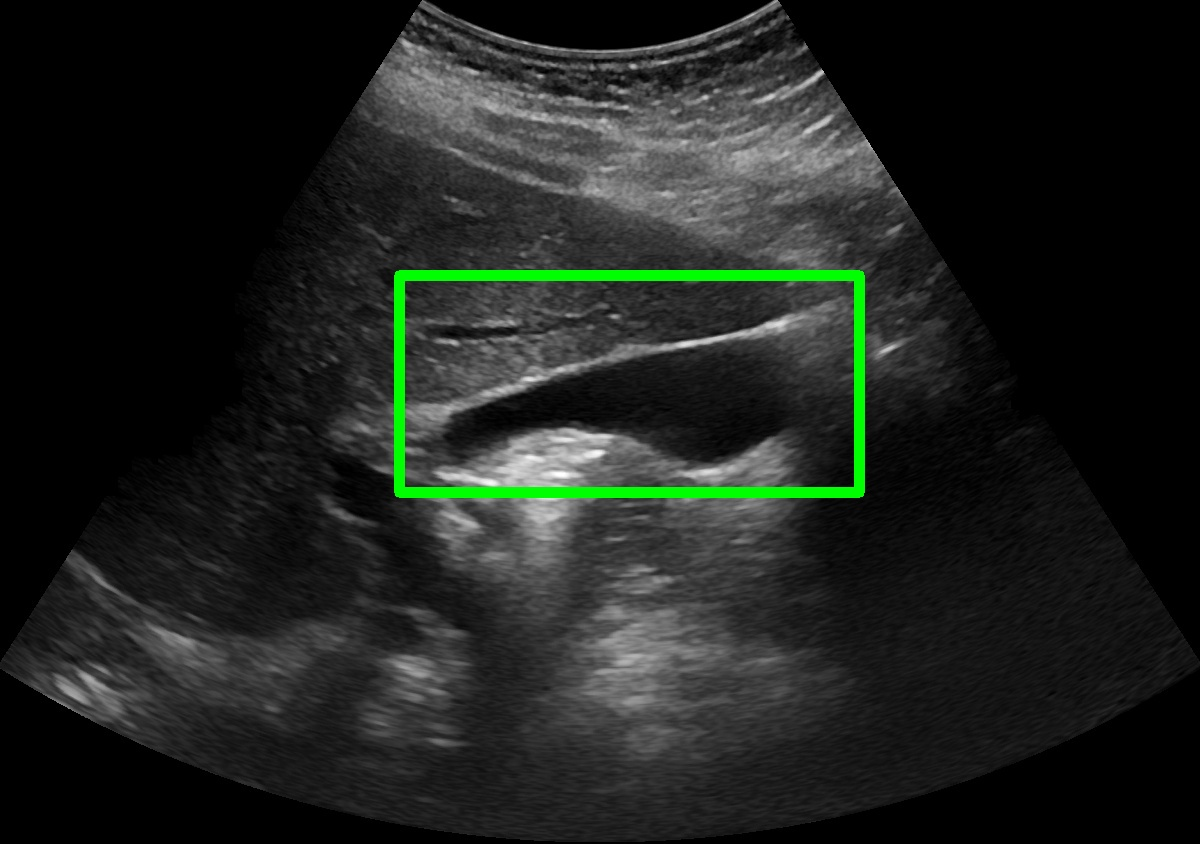
\includegraphics[width=\linewidth,height=10em]{figs/gbcnet/bbs-nml.png}
		\caption{}
	\end{subfigure}
    \begin{subfigure}[b]{0.3\linewidth}
		\centering
		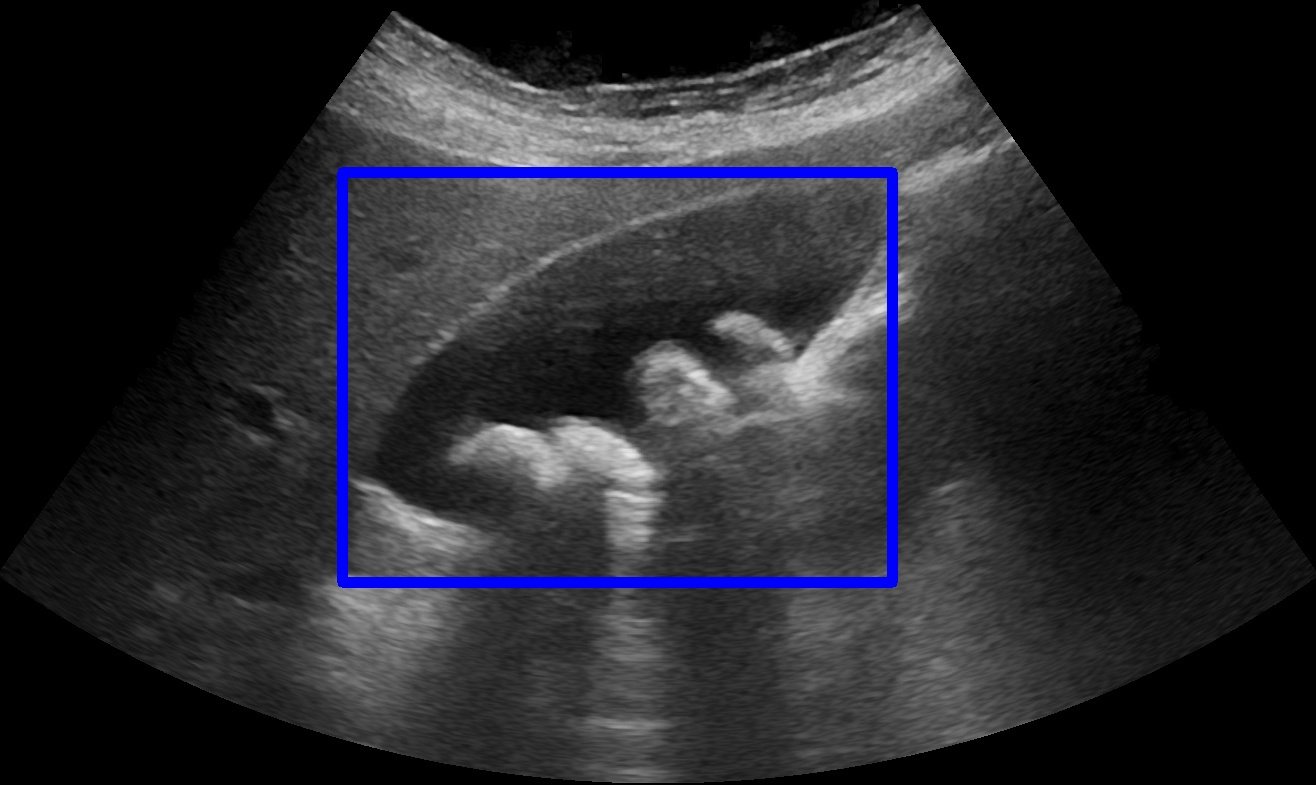
\includegraphics[width=\linewidth,height=10em]{figs/gbcnet/bbs-ben.png}
		\caption{}
	\end{subfigure}
    \begin{subfigure}[b]{0.3\linewidth}
		\centering
		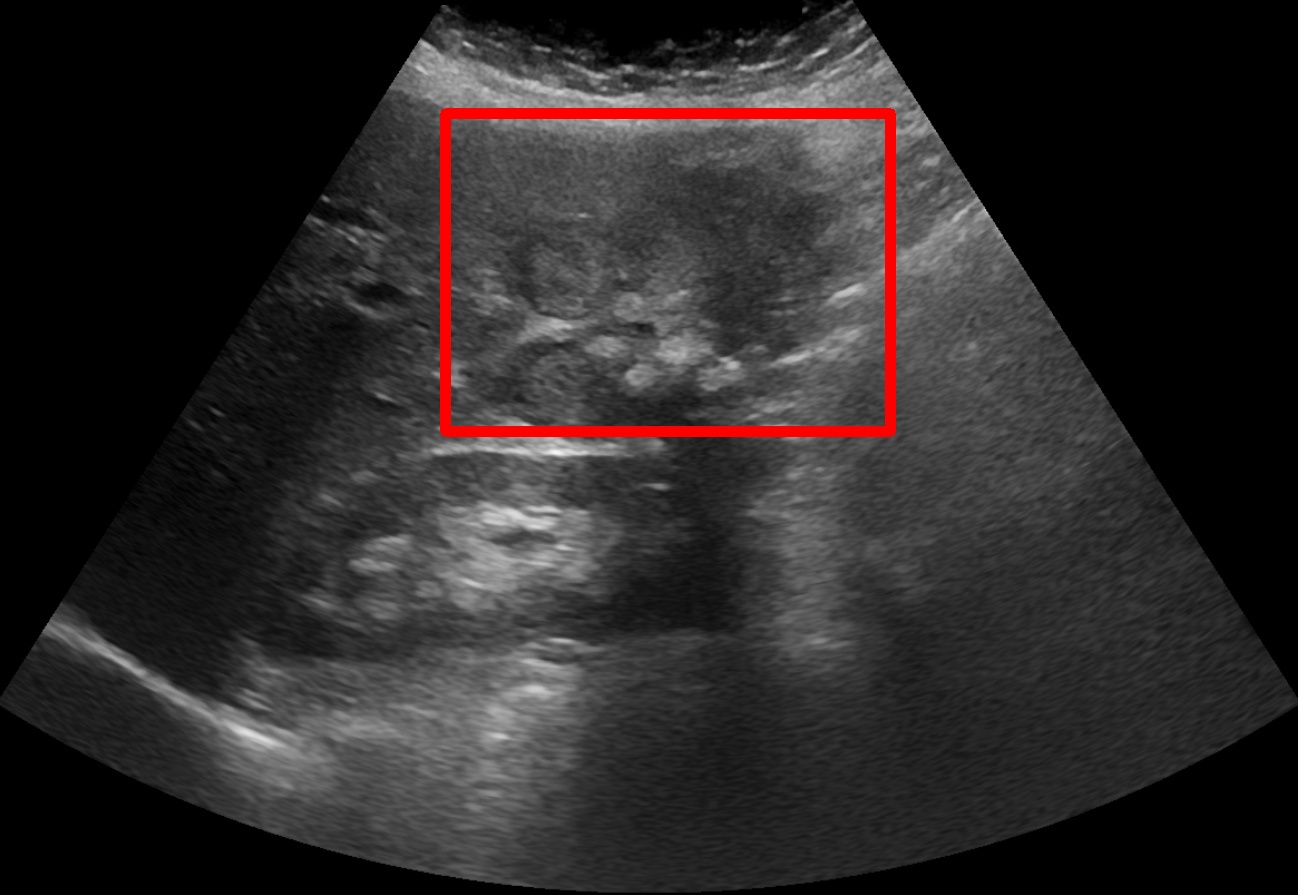
\includegraphics[width=\linewidth,height=10em]{figs/gbcnet/bbs-mlg.png}
		\caption{}
	\end{subfigure}
   \caption[Sample ROI annotation in USG images]{Sample ROI annotation. (a) Normal GB with ROI annotated in green, (b) GB with benign abnormalities with ROI in blue, and (c) Malignant GB with ROI annotated in red. }
    \label{fig:bb_sample}
\end{figure}
%
\subsection{Labeling and ROI Annotation}
%
Each image is labelled as one of the three classes - normal, benign, or malignant. These ground-truth classification labels were biopsy-proven to assert the correctness. Apart from image classification labels, we collected bounding-box annotations to capture the GB localization. Two expert radiologists with 10 and 2 years of experience in abdominal radiology did the bounding box labelling with consensus. Our radiologists used the LabelMe \cite{russell2008labelme} software to draw bounding boxes in the USG images of the dataset. In each image, the expert radiologists have drawn a single free-size axis-aligned bounding box spanning the entire \gb and adjacent liver parenchyma, preferably keeping the GB in the box's center to annotate the region of interest (\roi). \cref{fig:bb_sample} shows the sample \roi annotations drawn by the radiologists. For malignant cases, the \roi includes the visible malignant pathologies such as lesions, intraluminal polyp, mass, or malignant \gb wall thickening. 
%For the cases with no abnormality of the GB, the \roi contains the entire \gb. 

%\par In addition to the \roi, for the pathological GB cases, the %pathology was further highlighted using additional bouding boxes. Benign pathologies such as stones, benign wall thickening, benign polyp, sludge, and 
%regions containing the malignant pathologies such as lesion, intraluminal polyp, mass, or malignant \gb wall thickening were highlighted using axis-aligned bounding boxes covering only the pathological segment of the \gb. In the case of multiple anomalies in a single image, multiple boxes were drawn. 

\subsection{Dataset Statistics}
%
We have annotated 1255 abdominal \usg images collected from 218 patients from the acquired image corpus. Our dataset contains 71 patients with a normal gallbladder, 100 patients with benign abnormality, and 47 patients with malignancy. Overall, we have 432 normal, 558 benign, and 265 malignant images. The width of the images was between 801 and 1556 pixels, and the height was between 564 and 947 pixels. The variable size is due to cropping out of patient information from the Ultrasound image.

\subsection{Dataset Splits}
%
The sizes of the training and testing sets are 1133 and 122, respectively. To ensure generalization to unseen patients, all images of any particular patient were either in the train or the test split. The number of normal, benign, and malignant samples in the train and test set is 401, 509, 223, and 31, 49, and 42, respectively. Additionally, given the relatively small dataset, we report the 10-fold cross-validation metrics on the entire dataset for various experiments to assess generalization. All images of any particular patient appeared either in the training or the validation split during the cross-validation to guarantee the generalization to unseen patients.

% \begin{figure}
%     \centering
%     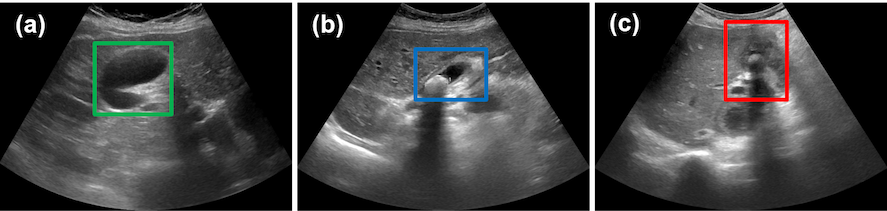
\includegraphics[width=\linewidth]{figs/radformer/annot-sample.png}
%     \caption{Sample ROI annotation. (a) Normal gallbladder with ROI in green, (b) benign GB with ROI in blue, and (c) malignant GB with ROI in red. }
%     \label{fig:data_sample}
% \end{figure}
%
%% DATASET
% \section{Dataset}
% %
% We have used the Gallbladder Cancer Ultrasound (GBCU) dataset \cite{basu2022surpassing}, publicly released by us in our previous work. For completeness, we provide a comprehensive description of the dataset in this section.

% \subsection{Data acquisition}
% %
% The patient data samples were acquired from the radiology department of the Postgraduate Institute of Medical Education \& Research (PGIMER, India). The patients were advised 8--8 hours of fasting before the examination for the adequate distension of the gallbladder. A Logic S8 machine (GE Healthcare) with a convex low-frequency transducer with a frequency of 1--5 MHz was used to capture the USG images. Radiologists having expertise in abdominal radiology assessed the patients from various positions and angles using subcostal and intercostal views for adequate visualization of the entire gallbladder, including its fundus, neck, and body. 
% A minimum of 10 Grayscale B-mode static images, including both sagittal and axial sections, were recorded for each patient.
% Colour Doppler, spectral Doppler, annotations, and measurements from the dataset are excluded. All personal textual information was removed from the images to anonymize them. 

% \subsection{Ground-truth labeling}
% %
% The biopsy reports of the patients are used to label each USG image as one of the three classes - normal, benign, or malignant. \radformer uses only these image-level labels during training. Apart from the image-level class labels, the bounding box annotations to locate the gallbladder and the surrounding ROI are also captured. It is important to note that we do not use these ROI bounding boxes during the training or inference of \radformer. 
% Two radiologists with 8 and 3 years of experience in abdominal radiology annotated the ROIs with consensus by using a single free-size axis-aligned box spanning the gallbladder and the adjacent regions. \cref{fig:data_sample} shows sample ROI annotations.

% \subsection{Statistics}
% %
% From the collected image corpus, the radiologists labeled 1255 USG images acquired from 218 patients. Our dataset contains 71 patients with a normal gallbladder, 100 patients with benign abnormality, and 47 patients with malignancy. Overall, the dataset contains 432 normal, 558 benign, and 265 malignant images. The images have a width of 801--1556 pixels and a height of 564--947 pixels. The variable size is due to cropping out of patient information from the image.

% \subsection{Dataset splits}
% %
% Given the relatively small dataset, we report 10-fold cross-validation metrics for various experimental models on the entire dataset. All images of any particular patient appeared either in the training or the validation split during the cross-validation to guarantee the generalization to unseen patients. Additionally we discuss the comparison with human experts using the GBCU test split containing 122 images (31 normal, 49 benign, and 42 malignant).


% subsection{In-house US Dataset for Gallbladder Cancer}
% %
% The transabdominal US video dataset is acquired at the Postgraduate Institute of Medical Education and Research (PGIMER), Chandigarh, India. The PGIMER ethics committee approved the study.

\section{Video Data}
\label{data:gbusv}
%
\subsection{Collection and Curation}
We have curated the video data in two phases. In the first phase, we collected 32 malignant and 32 non-malignant videos containing a total of 12,251 and 3,549 frames, respectively. 
%Radiologists with 2-8 years of experience in abdominal sonography acquired the data. The US videos were obtained after at least 6 hours of fasting using a 1--5 MHz curved array transducer (C-1-5D, Logiq S8, GE Healthcare). The scanning intended to include the entire GB and the lesion or pathology. The frame rate was 29 fps. 
%Note that we do not use video-level labels in our setup. 
We cropped the video frames from the center to anonymize the patient information and annotations. The processed video frames were of size $360\!\times\!480$ pixels. \cref{usucl_fig:data_sample} shows some samples from the video data. We have released this large-scale video dataset for the community as a part of our published work \cite{basu2022unsupervised}. We call this dataset Gallbladder Ultrasound Video (GBUSV) dataset. GBUSV was primarily used for the unsupervised contrastive pretraining for GBC representation learning discussed in \cref{chap:limited}. The video labels were not used during the contrastive pretraining.

% \mypara{Image Data}
% %
% We use the publicly contributed GBCU dataset \cite{basu2022surpassing} consisting of 1255 US images from 218 patients. The dataset consists of 990 non-malignant (171 patients with normal and benign GB) and 265 malignant (47 patients) GB images. The images were labeled as normal, benign, or malignant, and such labels were biopsy-proven. We use this dataset for finetuning and report 10-fold cross-validation. 
% %We did the cross-validation splits at the patient level, and all images of any patient appeared either in the train or validation split. 
% Note that the patients recorded in the video dataset are not included in this image dataset to ensure generalization. 


\begin{figure}[t]
    \centering
    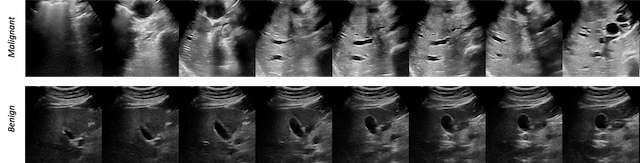
\includegraphics[width=\linewidth]{figs/focusmae/us_video.png}
    \caption[Video data samples]{Sample video sequences from our US video dataset used for GBC detection. We show samples of both malignant and benign (non-malignant) sequences for GBC video data. }
    \label{fig:video_data_sample}
\end{figure}

% 
In the second phase, we utilized the public GBUSV dataset and extended it with an additional set of USG videos collected by our team of radiologists. The extended dataset was used for developing and assessing video-based GBC detection models discussed in \cref{chap:focusmae}. We relied on the biopsy reports of the patients for labelling the videos. The GBUSV dataset comprises 64 Gallbladder US videos, with 32 labelled as benign and another 32 labelled as malignant. We added 27 additional US videos specifically depicting Gallbladder malignancy to the GBUSV dataset for curating the video dataset suitable for the video-based \gbc detection task. 
\cref{fig:video_data_sample} shows two sample video sequences, one belonging to a malignant patient, and the other collected from a patient with non-malignant \gb.
%We obtained video samples from patients referred to a tertiary care referral hospital for abdominal US examinations targeting suspected Gallbladder pathologies. Each patient provided informed written consent during recruitment, and we ensure patient privacy by fully anonymizing the data. The institute Ethics Committee approved the study. Patients were fasting for a minimum of 6 hours to ensure adequate distention of the \gb. Our team of radiologists employed a 1-5 MHz curved array transducer (C-1-5D, Logiq S8, GE Healthcare) for the scanning process. The scanning protocol covers the entire gallbladder (including fundus, body, and neck) and any associated lesions or pathologies. We cropped the video frames from the center to safeguard patient privacy and annotations. The processed frames have a size of 360x480 pixels. \cref{focusmae_fig:data_sample} shows sample sequences from the dataset. 

%\subsection{Annotation}
%%
%We relied on the GB biopsy reports for labeling the videos. %Additionally, two radiologists with 2 and 10 years of expertise in abdominal ultrasound (US), were consulted to draw bounding boxes covering the entire GB and the adjacent liver parenchyma in the frames where malignant lesion is visible. 
%The radiologists were pinpoint frames exhibiting clinical signs of malignancy. 
%In cases of malignant videos, the radiologists reached a consensus to label each frame as either malignant or non-malignant. 
%Although these frame-level annotations aren't directly employed for training video-based detection methods, they play a crucial role in qualitatively assessing the detectors. Moreover, these annotations hold potential for frame-level Video Anomaly Detection tasks. 
%Additionally, in each video, the radiologists have drawn an axis-aligned bounding box covering the entire GB and adjacent liver parenchyma to annotate the Region-of-Interest (ROI) that may contain the malignancy.

\subsection{Dataset Statistics}
%
The video dataset comprises 59 malignant and 32 non-malignant videos, collected from 41 malignant and 32 benign patients, respectively. The length of the videos varied from 43 to 888 frames. In total, the dataset encompasses 21,955 frames, with 18,406 frames attributed to videos labelled as malignant and 3,549 frames attributed to benign (non-malignant) videos. %Among these, radiologists identified 3212 frames exhibiting definite signs of malignancy. 

\subsection{Dataset Splits for Video-based GBC Detection}
%
We use the 5-fold cross-validation for the complete video dataset for key experiments in the video-based detection task. The cross-validation splits were conducted on a patient-wise basis, ensuring that all videos of a particular patient appeared exclusively in either the training or the validation split during cross-validation. Recall that the original GBUSV video dataset collected in the first phase did not contain any splits.

\chapter{Developing an Accurate GBC Detector}
%
\label{chap:gbcnet}
%
In this chapter, we systematically explore the potential of Deep Convolution Neural Network (CNN) models for accurately detecting Gallbladder Cancer (GBC) from Ultrasound (USG) images. As outlined in \cref{chap:intro}, USG is the predominant diagnostic modality for gallbladder (GB) diseases due to its affordability and accessibility. However, the analysis of USG images for GBC detection presents challenges such as low image quality, noise, and varying viewpoints resulting from the handheld nature of the sensor. To address these challenges, we introduce GBCNet and a curriculum tailored to enhance GBC detection performance from USG. We present a comprehensive discussion on GBCNet and the curriculum in this chapter.
\par The contents of this chapter was published as the following paper:
\par [1] \textit{Soumen Basu, Mayank Gupta, Pratyaksha Rana, Pankaj Gupta, and Chetan Arora. ``Surpassing the human accuracy: detecting gallbladder cancer from USG images with curriculum learning.'' In Proceedings of the IEEE/CVF Conference on Computer Vision and Pattern Recognition (CVPR), pp. 20886-20896, 2022}.

\section{Introduction}
%
Gallbladder cancer (GBC) is characterized by its aggressive nature, progressing rapidly if left untreated. Often, the disease advances silently, with malignancy extending into the neighboring liver and subsequently spreading to distant organs (called metastasis). Early diagnosis and resection are critical for improving the survival rate of \gbc. USG, on the other hand, stands out as the predominant diagnostic imaging modality for investigating patients with suspected gallbladder ailments \cite{klibanov2015ultrasound}, making it an excellent candidate modality for early detection of GBC. The advantages of USG include its affordability, accessibility, absence of ionizing radiation, and portability. Particularly in low-resource countries, the access to CT or MRI is limited due to high costs and their availability is also restricted to a few selected care centers. USG proves to be an invaluable diagnostic tool for early detection and intervention to GBC in such low-resource settings.

\par While identifying anomalies like stones or thickening of the GB wall during routine ultrasound (USG) is straightforward, precise characterization wall thickening remains challenging for even the most experienced radiologists \cite{gbc-lancet, gb-rads-paper, gupta2020imaging}. Although GBC typically presents with irregular wall thickening, early stages may exhibit smooth and symmetric thickening, which is similar to benign conditions \cite{gupta2020imaging}. As discussed earlier in \cref{sec:clinical}, traditional signs of benign thickening, such as echo-layering, can be present in malignant cases, complicating diagnosis. Moreover, various other medical conditions, including acute cholecystitis and hepatic, renal, and heart issues, can also cause gallbladder wall thickening, further complicating differentiation between benign and malignant causes. Frequently, USG is the only diagnostic imaging conducted for patients with suspected GB ailments. In cases where malignancy is not suspected, further testing is typically omitted, potentially allowing GBC to progress silently. Hence, there is an imperative need to develop effective characterization for GB malignancy from USG images. In pursuit of this objective, we turn to automated deep convolutional neural network (CNN)-based methods for gallbladder cancer (GBC) detection. Recent advancements in CNN-based machine learning (ML) models have yielded transformative progress in radiology and the diagnosis of various diseases, including breast cancer, lung cancer, pancreatic cancer, and melanoma \cite{ardila2019end, bejnordi2017diagnostic, chu2019application, codella2017deep, han2017breast}. However, the utilization of such models for GBC detection is notably absent. While prior efforts have focused on the segmentation and detection of GB abnormalities such as stones and polyps \cite{gbPolyp, gbPolyp2, gbAutomatic}, the specific detection of GBC from USG has not been attempted in prior literature.

\par However, there are significant challenges in using \cnn models for accurately detecting GBC from \usg image as discussed in \cref{sec:challenges}. %Unlike \mri or \ct, \usg images suffer from low imaging quality due to noise and other sensor artifacts such as acoustic shadow and echogenic textures as discussed in \Cref{sec:usg_artifact_issue}. The views are also not aligned due to the handheld nature of the sensor. 
Our study of state-of-the-art (\sota) CNN-based image classification techniques reveal that they often fail to learn the salient \gb region due to the presence of shadows, which may have similar visual traits of a \gb in \usg images (\cref{fig:teaser}). In addition to shadows, \gbc detection also gets biased towards learning from spurious textures due to noise and adjacent organ tissues rather than the shape or boundary of \gb wall, which impedes the accurate detection of GBC and results in poor GBC detection by off-the-shelf CNN models. Further, unlike normal and benign \gb regions, which have regular anatomy, malignant cases are much harder to detect precisely due to the absence of a clear \gb boundary or shape and the presence of a mass. %The lack of annotated dataset adds to the challenge of training the CNN models.

\begin{figure}[t]
    \centering
    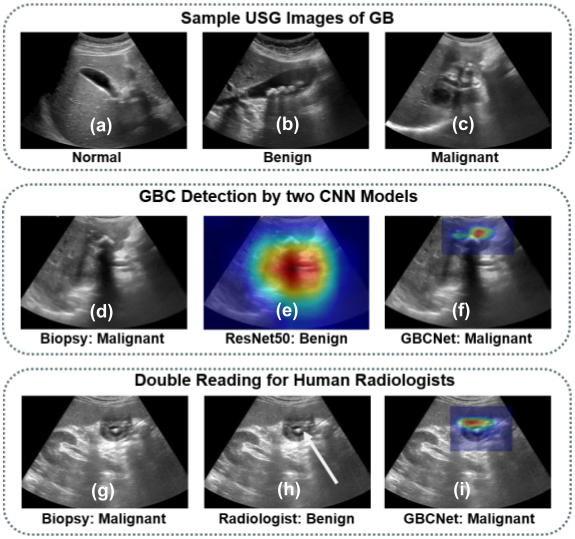
\includegraphics[width=0.6\textwidth]{figs/gbcnet/teaser.png}
    \caption[Depiction of issues with USG-based GBC detection]{(a), (b), and (c) Normal, benign, and malignant \gb sample in \usg images, respectively. While normal or benign \gb have regular anatomy, clear boundary is absent in malignant \gb. (d) A malignant (biopsy-proven) \gb sample. (e) Shadows having visual traits of a \gb leads to localization error in ResNet50. (f) \gbcnet tackles shadow artifacts well. (g) Another sample of malignant \gb. (h) The radiologist incorrectly diagnosed the \gb as benign based on the stone and wall thickening. (i) \gbcnet helps the radiologist to identify the salient region with liver infiltration by the \gb, a critical feature of \gbc, and correct the prediction.}
    \label{fig:teaser}
\end{figure}

\par In addressing this gap, we present the following significant contributions aimed at achieving highly accurate gallbladder cancer (GBC) detection from ultrasound (USG). Our primary goal is to ensure that our model exhibits a high recall (sensitivity) in detecting GBC. This emphasis on high recall is crucial as false negatives, where malignant cases are incorrectly predicted as non-malignant, can have severe consequences for the patients. On the other hand, the false positive prediction of malignancy can impose significant clinical, financial, and emotional burdens on the patients. It is thus essential to ensure that the model also shows high specificity (true negative rate).

%We propose GBCNet to tackle the challenges in our problem. GBCNet first extracts the regions of interest (\rois) by detecting the \gb (and not the cancer), and then uses a new multi-scale, second-order pooling architecture specializing in classifying \gbc. To effectively handle spurious textures, we propose a curriculum inspired by human visual acuity, which reduces the texture biases in GBCNet. Experimental results demonstrate that GBCNet significantly outperforms \sota \cnn models, as well as the expert radiologists. Our technical innovations are generic to other \usg image analysis tasks as well. Hence, as a validation, we also show the efficacy of GBCNet in detecting  breast cancer from \usg images. 
%Project page with source code, trained models, and data is available at \url{https://gbc-iitd.github.io/gbcnet.html}
\noindent \mypara{Contributions:}
\begin{enumerate}%[label=\textbf{(\arabic*)}]
	\item We focus on circumventing the challenges for automated detection of \gbc from \usg images and propose a deep neural network, GBCNet, for detecting \gbc from \usg images. GBCNet first extracts candidate regions of interest (\rois) by detecting the \gb (and not the cancer) from the \usg to mitigate the effects of shadows. Following the \roi detection, GBCNet employs a new  multi-scale, second-order pooling-based (MS-SoP) classifier on the \rois to classify gallbladder malignancy. MS-SoP encodes rich feature representations for malignancy detection. Experimental results demonstrate that GBCNet significantly outperforms multiple \sota \cnn models, as well as the expert radiologists. 
	%
	\item Even though GBCNet shows improvement in \gb malignancy detection over the \sota models, the spurious texture present in an \roi bias the classification unit towards generating false positives. To alleviate the issue, we propose a training curriculum inspired by human visual acuity \cite{kwon2016compensation, vogelsang2018VisualAcuity}. Visual acuity refers to the sharpness of visual stimuli. Studies suggest that an initial period of low visual acuity followed by high visual acuity helps the visual cortex in humans to formulate a better receptive field and emphasizes features such as shape or structure while identifying objects. 
	The proposed curriculum mitigates texture bias and helps GBCNet focus on shape features important for accurate \gbc detection from \usg images. % We validate the same in the context of \gbc detection from \usg images. %only, where we show in our experiment that our model after training with the proposed curriculum better focuses on GB boundaries.
	%
	\item A lack of publicly available \usg image datasets related to \gb malignancy adds to the difficulty of utilizing \cnn models for detecting \gbc. As discussed in \Cref{chap:data}, we have collected, annotated, and curated a \usg image dataset of 1255 abdominal \usg images. The dataset is referred as the Gallbladder Cancer Ultrasound (GBCU) dataset, and was publicly released with this work.
	%The dataset is available to the community.
	%post-acceptance of the paper after signing the necessary privacy agreement with our hospital. 	
\end{enumerate}


%
\section{Introduction}
%
According to GLOBOCAN 2018 \cite{bray2018global}, worldwide about 165,000 people die of \gbc annually. For most patients, \gbc is detected at an advanced stage, with a mean survival rate for patients with advanced \gbc of six months and a 5-year survival rate of 5\% \cite{randi2006gallbladder, gupta2021locally}. Detecting \gbc at an early stage could ameliorate the bleak survival rate. 

Lately, machine learning models based on convolutional neural network (\cnn) architectures have made transformational progress in radiology, and medical diagnosis for diseases such as breast cancer, lung cancer, pancreatic cancer, and melanoma \cite{ardila2019end, bejnordi2017diagnostic, chu2019application, codella2017deep, han2017breast}. However, their usage is conspicuously absent for the \gbc detection. Although there has been prior work involving segmentation and detection of the \gb abnormalities such as stones and polyps \cite{gbPolyp, gbPolyp2, gbAutomatic}, detection of \gbc is missing from the list. A search on Google Scholar with keywords ``artificial intelligence'' and ``gallbladder cancer'' returned 204 articles between 2015-2021. In these, we did not find any published article on deep learning-based \gbc detection from \usg images.

%\par According to GLOBOCAN 2018, GBC causes 165,087 deaths and 219,420 incidences every year worldwide \cite{armitage2014abeloff, bray2018global}. 
%%GBC is one of the leading causes of cancer-related deaths among Indian women \cite{randi2006gallbladder, bray2018global}. 
%The disease is prevalent in China, India, and Latin America. Canada, Australia, USA, and Europe also face a high incidence of GBC. 
%%\figref{fig:sec1-1} shows the detailed distribution of the incidence rate around the world.  
%GBC is detected at an advanced and metastasized stage for most patients, impeding curative resection and resulting in a dismal prognosis \cite{randi2006gallbladder, gupta2021locally}. 
%The overall mean survival rate for patients with advanced GBC is six months, with a 5-year survival rate of 5\%. 
%%In the USA, only about 1 in every 5 cases of GBC are identified in an early stage \cite{howlader2017seer}.
 
Early diagnosis and resection are critical for improving the survival rate of \gbc. Due to the non-ionizing radiation, low cost, portability, and accessibility, \usg is a popular diagnostic imaging modality. Although identifying anomalies such as stones or \gb wall thickening at routine \usg is easy, accurate characterization of the wall thickening is challenging \cite{gupta2020imaging, gb-rads-paper}. Often, \usg is the sole diagnostic imaging performed for patients with suspected \gb ailments. If malignancy is not suspected, no further testing is usually performed, and \gbc could silently advance. Therefore, it is imperative to develop and understand the characterization of \gb malignancy from \usg images.

There are significant challenges in using \cnn models for \usg image analysis. Unlike \mri or \ct, \usg images suffer from low imaging quality due to noise and other sensor artifacts. The views are also not aligned due to the handheld nature of the sensor. We observe that modern \cnn classifiers fail to localize the salient \gb region due to the presence of shadows which often have similar visual traits of a \gb in \usg images (\cref{fig:teaser}). Training object detectors for \gbc detection gets biased towards learning from spurious textures due to noise and adjacent organ tissues rather than the shape or boundary of \gb wall, which results in poor accuracy. Further, unlike normal and benign \gb regions, which have regular anatomy, malignant cases are much harder to detect due to the absence of a clear \gb boundary or shape and the presence of a mass.

\mypara{Contributions} 
%
The key contributions of this work are:
%\vspace{-0.5em}
\begin{enumerate}%[label=\textbf{(\arabic*)}]
%\itemsep-0.5em
	\item We focus on circumventing the challenges for automated detection of \gbc from \usg images and propose a deep neural network, GBCNet, for detecting \gbc from \usg images. GBCNet extracts candidate regions of interest (\rois) from the \usg to mitigate the effects of shadows and then uses a new  multi-scale, second-order pooling-based (MS-SoP) classifier on the \rois to classify gallbladder malignancy.
    %The first two stages of GBCNet are inspired by two-stage object detectors but focus only on detecting the \gb (and not cancer) and selecting a focused region of interest (\roi) to mitigate the effects of shadows. The third stage uses a new multi-scale, second-order pooling (MS-SoP) architecture to classify gallbladder malignancy.
	MS-SoP encodes rich feature representations for malignancy detection. 
	%
	\item Even though GBCNet shows improvement in \gb malignancy detection over multiple \sota models, the spurious texture present in an \roi bias the classification unit towards generating false positives. To alleviate the issue, we propose a training curriculum inspired by human visual acuity \cite{kwon2016compensation, vogelsang2018VisualAcuity}. Visual acuity refers to the sharpness of visual stimuli. %Studies suggest that an initial period of low visual acuity followed by high visual acuity helps the visual cortex in humans to formulate a better receptive field and emphasizes features such as shape or structure while identifying objects. 
	The proposed curriculum mitigates texture bias and helps GBCNet focus on shape features important for accurate \gbc detection from \usg images.% We validate the same in the context of \gbc detection from \usg images. %only, where we show in our experiment that our model after training with the proposed curriculum better focuses on GB boundaries.
	%
	\item A lack of publicly available \usg image datasets related to \gb malignancy adds to the difficulty of utilizing \cnn models for detecting \gbc. We have collected, annotated, and curated a \usg image dataset of 1255 abdominal \usg images collected from 218 patients. We refer this dataset as the Gallbladder Cancer Ultrasound (GBCU) dataset.
	%The dataset is available to the community.
	%post-acceptance of the paper after signing the necessary privacy agreement with our hospital. 	
\end{enumerate}

%

\section{Related Work}

\myfirstpara{Deep Learning for GB Abnormalities}
%
\usg imaging is an effective modality for diagnosing \gbc and related \gb afflictions \cite{yuan2018gbcManual}. 
%Recently, deep learning has been used as a diagnostic tool in medical imaging to great effect \cite{litjens2017dlmedical}. 
%Multiple studies have shown the application of these techniques on GB-related ailments, such as the detection of GB stones, biliary artesia, cholecystitis, and polyps. 
Lien \etal \cite{gbAutomatic} use a parameter-adaptive pulse-coupled neural network for \gb stone segmentation in \usg images. Pang \etal \cite{gbYolo} identify \gb and gallstones using a YOLOv3 model from \ct images. %Chen \etal \cite{gbPolyp} suggest an approach that segments the GB region followed by an AdaBoost classifier for diagnosing polyps. 
Jeong \etal \cite{gbPolyp2} uses an InceptionV3 model to classify neoplastic polyps from cropped samples of \gb \usg images. \gbc is a serious problem affecting a significant number of people. Despite the presence of numerous studies on using deep learning on other \gb-related afflictions, there is an absence of any work that applies deep learning to \gbc detection.

\mypara{Deep Learning for USG}
%
\cnn models have been widely applied in a plethora of \usg-based imaging tasks.
Mishra \etal proposed a fully convolutional neural network with deep attentional supervision on USG images for segmentation of blood vessel, liver lumen, and lesion \cite{mishra2018USSegmentation}. Deep learning-based segmentation models such as U-Net or Link-Net have been used to measure head circumference in fetal USG images \cite{budd2019FetalHC, sobhaninia2019FetalHC}. %VGG16-based architectures have been used for detecting the fetal scan plane \cite{baumgartner2017PlaneDetection}. 
Azizi \etal proposed a Deep Belief Network for detecting prostate cancer from USG images \cite{azizi2015ultrasound}. Li \etal modified Faster-RCNN for improving the detection of papillary thyroid cancer from USG \cite{li2018improved}. Deep learning has also been used in ovarian cancer \cite{zhang2019improved}, metastatic lymph node \cite{lee2018deep}, and breast cancer detection \cite{almajalid2018development, becker2018classification, cao2019BreastLesion, yap2018breast}. Zhu \etal recently proposed an attention-guided second-order sub-region pooling network for exploiting higher-order correlation to extract complex features from USG images \cite{zhu2020second}. A study by Ning \etal implemented a multi-scale higher-order pooling-based solution for breast lesion classification on USG images \cite{ning2020multi} .
%\cnn models have been widely applied in \usg imaging tasks, such as ovarian cancer detection \cite{zhang2019improved}, breast cancer region, mass and boundary detection \cite{bian2017boundary, cao2019BreastLesion, yap2018breast, ning2020multi, zhu2020second}, measuring head circumference in fetal \usg images \cite{sobhaninia2019FetalHC, budd2019FetalHC}. %, and other medical imaging and diagnostic applications. 

%\cite{mishra2018USSegmentation} proposed a fully convolutional neural network with deep attentional supervision on USG images for segmentation of blood vessel, liver lumen, and lesion. Deep learning-based segmentation models such as U-Net or Link-Net have been used to measure head circumference in fetal USG images \cite{sobhaninia2019FetalHC, budd2019FetalHC}. VGG16-based architectures have been used for detecting the fetal scan plane \cite{baumgartner2017PlaneDetection}. \cite{azizi2015ultrasound} proposed a Deep Belief Network for detecting prostate cancer from USG images. \cite{li2018improved} suggested modifications to Faster-RCNN for improving the detection of papillary thyroid cancer from USG. Deep learning has been used in ovarian cancer \cite{zhang2019improved}, metastatic lymph node \cite{lee2018deep}, and breast cancer detection \cite{cao2019BreastLesion, yap2018breast, almajalid2018development, becker2018classification}. \cite{zhu2020second} suggested an attention-guided second-order sub-region pooling network for exploiting higher-order correlation to extract complex features from USG images. A study by \cite{ning2020multi} proposes a multi-scale higher-order pooling-based solution for breast lesion classification on USG images. \cite{wang2020auto} used reinforcement learning to auto-assign weights to multimodal USG framework. 

\mypara{Curriculum Learning}
%
Curriculum learning has been applied to different medical imaging tasks. While Jesson \etal \cite{jesson2017cased} used a patch-based curriculum for lung nodule detection, Tang \etal \cite{tang2018attention} used disease severity level to identify thoracic diseases from chest radiographs. Oksuz \etal \cite{oksuz2019automatic} proposed image corruption-based curriculum to detect motion artifacts in cardiac \mri. 

\mypara{Texture Bias in Neural Networks}
%
Presence of mass and a thickened \gb wall are prominent indicators of \gb abnormality. However, typical \cnn-based architectures are biased towards textures rather than shape \cite{geirhos2018Texture}. This may lead GBCNet to focus on soft tissue textures such as liver rather than noticing cues based on the shape and wall of the \gb. 
%Therefore, a strategy is needed to reduce this texture bias of the network. 
Multiple works have attempted to reduce texture bias and improve the spatial understanding of a model. Geirhos \etal \cite{geirhos2018Texture} suggest style transfer to replace the original texture of images while Brendel \etal \cite{brendel2019BagOfFeatures} propose a method similar to a Bag of Features model to force spatial learning. 

\mypara{Visual Acuity in Learning Models}
%
Vogelsang \etal \cite{vogelsang2018VisualAcuity} suggest that a period of low visual acuity (blurred vision) followed by high visual acuity induces better spatial processing and also increases the receptive field in human vision. 
%Some recent works seem to follow the broad strategy and overcome the texture bias problem using blurring or similar other operations. 
Different from our visual acuity-inspired strategy of working with input space, Sinha \etal \cite{sinha2020curriculumBySmoothing} propose applying a Gaussian kernel on the output feature map of every layer of a network. The use of blurring before pooling seems to mitigate aliasing effects due to sub-sampling in the pooling layer rather than the use of visual acuity. Azad \etal \cite{azad2020textureDoG} have integrated a Difference of Gaussian (DoG) operation into their model. Similar to \cite{sinha2020curriculumBySmoothing}, they end up attenuating the high frequency in the feature maps corresponding to every layer rather than the input image, for which there is no obvious biological connection known. On the other hand, our proposed visual acuity-based curriculum works in the input space and has a solid neural basis \cite{vogelsang2018VisualAcuity}.


\begin{figure}[t]
	\centering
	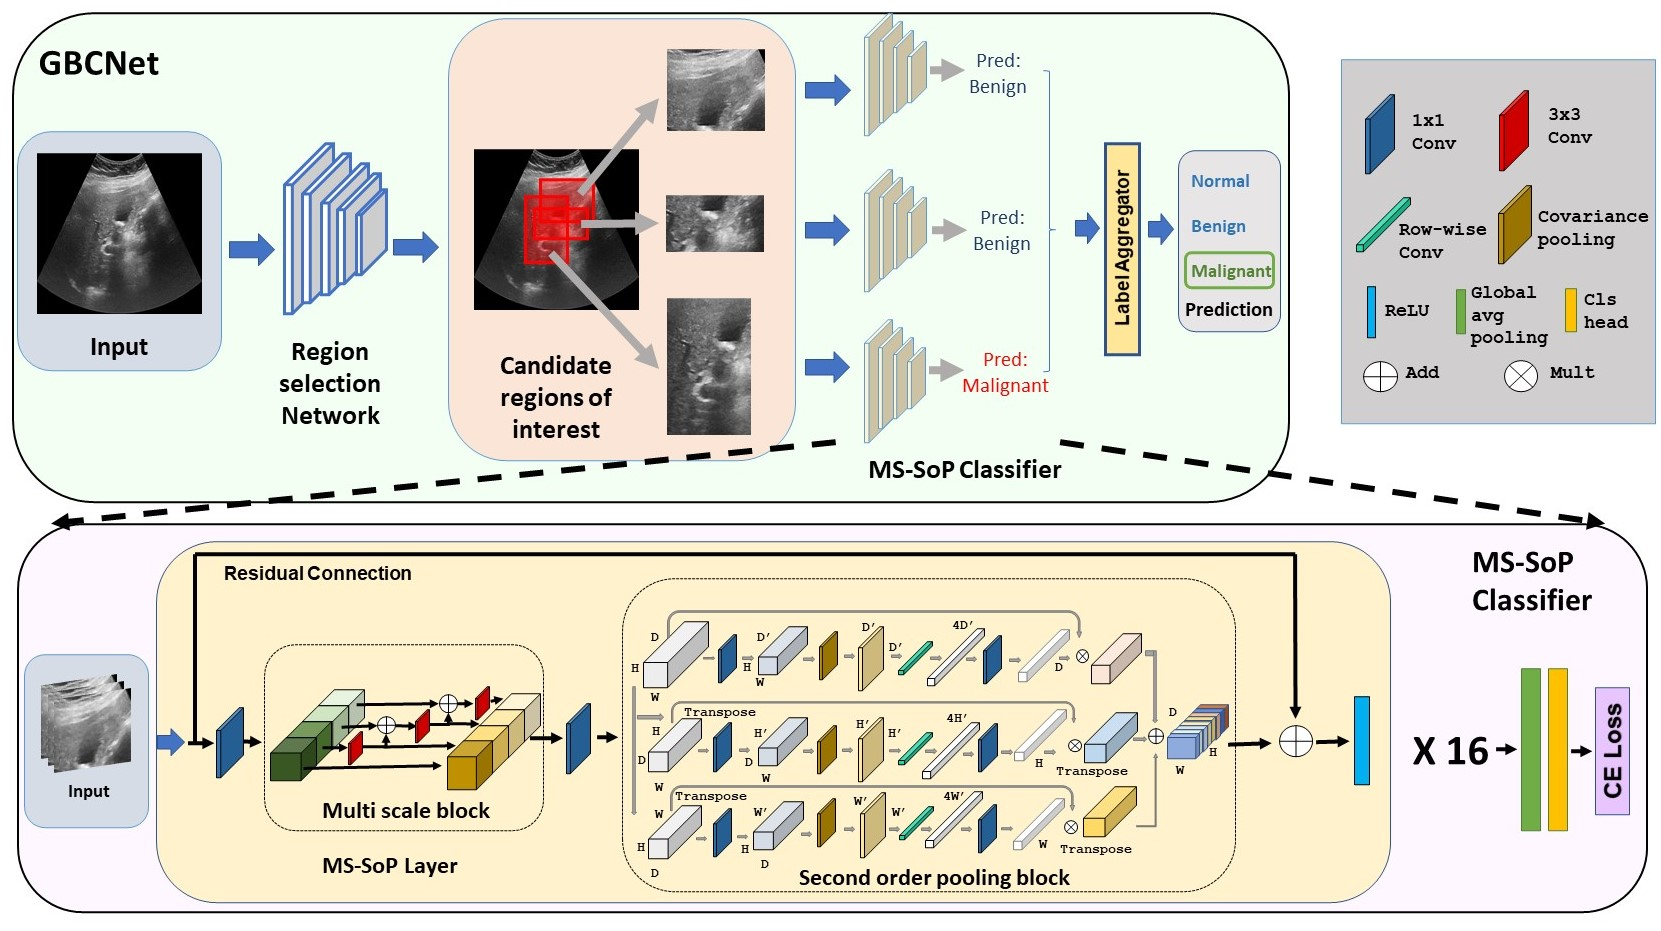
\includegraphics[width=\textwidth]{figs/gbcnet/arch-compact.jpg}
	\caption[Architecture of GBCNet]{Overview of the \gbcnet architecture. The region selection network localizes the candidate regions of interest and the multi-scale, second-order pooling-based (MS-SoP) classifier at the next stage predicts malignancy for each region. The predictions for each region is aggregated to get the final prediction on the whole image.}
	\label{fig-arch-overview}
\end{figure}


\section{Our Method}
%
\subsection{GBCNet: Model Architecture}
%
%Unlike CT or MRI, \usg images suffer from much higher noise levels and artifacts such as shadow due to \gb stones. 
The artifacts in \usg images often result in multiple spurious areas in a \usg image with very similar visual traits as the \gb region, leading to a disappointing performance by the baseline classifiers. 
%We have developed a CNN-based model, referred to as GBCNet, which can successfully detect \gbc, despite all the challenges described above. 
GBCNet selects candidate regions of interest (\rois) from the \usg to mitigate the influence of spurious artifacts like shadows and then uses a multi-scale, second-order pooling-based (MS-SoP) classifier on the \rois. \cref{fig-arch-overview} presents a conceptual diagram of the architecture. 
%We train a deep object detector to localize the \gb in the \usg images and generate the candidate ROIs to mitigate the influence of spurious artifacts. 
%The ROIs are cropped from the RGB images and passed to the MS-SoP classifier, to predict \gb malignancy.
At test time, the detector may predict multiple \rois overlapping with the \gb. Occasionally, the detection network may fail to localize the \rois. In this case, we pass the entire image to the classifier. The proposed MS-SoP classifier exploits a range of spatial scales 
%through multiple receptive fields during the feature encoding. In addition, the classifier utilizes 
and second-order statistics to generate rich features from \usg images to learn the characteristics of malignancy. We run the classifier for each candidate region during inference and aggregate the predicted labels to compute the prediction for the entire image. If any of the \rois is classified as malignant, the image as a whole is classified as malignant. If all the regions are predicted to be normal, the image is classified as normal. In all other cases, the image is predicted to be benign. 
%\par We observe that the above configuration of \gbCNet, though improving the detection of malignancy, still has a high false-positive rate. Our analysis shows that this is due to the texture bias of neural network models, which has been reported for the natural images as well \cite{geirhos2018Texture}. Inspired by human visual acuity, we propose a novel customized curriculum training regimen for training the classifier module of GBCNet. The proposed training process mitigates the texture bias and helps GBCNet reach the reported performance level. In the following subsections, we discuss different components of the GBCNet.

\mypara{Candidate \roi Selection}
%
We used deep object detection networks to localize the \gb region in a \usg image. The predicted bounding boxes serve as candidate regions of interest and mitigate the adverse effect of noise and artifacts from non-\gb regions during the classification. For training the \roi selection models, we use only two classes - background and the \gb region. In this stage, we only detect the \gb and do not classify them as malignant or non-malignant. In principle, it is possible to do both in a single stage, but we observed 
%that the candidate regions suggested by first stage region proposal network are often shifted from the \gb region, and classifying malignancy based upon them leads to poorer results. After the second stage the regions gets refined to a greater accuracy, and we observed 
that using a separate classifier on the focused \rois leads to better accuracy. We note that our findings regarding the superiority of using classification on focused regions, instead of over the entire image, are consistent with other recent works \cite{lancet_pancreas, cao2019BreastLesion, fan2020inf, sirinukunwattana2016locality, eccv2020_devil_in_classification}. Prior studies demonstrate that modern object detection architectures such as YOLO \cite{yolov4} or Faster-RCNN \cite{fasterrcnn} can detect breast lesions in \usg images  \cite{cao2019BreastLesion}. On the other hand, recently proposed anchor-free approaches, such as Reppoints \cite{reppoints}, and CentripetalNet \cite{centripetalnet} can detect unconventionally sized objects such as \gb. Hence, we experimented with all the above approaches for \roi selection in our framework. 

\mypara{MS-SoP Classifier}
%
Feature extraction in deep neural networks typically rely on first-order statistics, which performs unsatisfactorily in modalities like \usg. The presence of noise and artifacts along with ambiguous organ boundaries add to the complexities of detecting \gbc from \usg images. 
Modeling higher-order statistics has gained popularity in recent years due to its enhanced ability to capture complex features and non-linearity in deep neural networks \cite{gao2019global, li2017second, zoumpourlis2017non}. %The presence of noise and artifacts along with ambiguous organ boundaries add to the complexities of detecting \gbc from ultrasound images. 
Ning \etal \cite{ning2020multi} recently used higher-order feature fusion for classifying breast lesions. They have used RGB image patches of three fixed scales at the input layer. We take the idea further and develop a novel multi-scale, second-order pooling (MS-SoP) layer to encode rich features suitable for malignant \gb detection. In contrast to \cite{ning2020multi}, we exploit feature maps of multiple scales in all the intermediate layers to learn a rich representation. The proposed MS-SoP layers can be conveniently plugged into any \cnn backbone.
%Further, instead of using the features at different resolutions, we use the multiple receptive fields to capture features at different scales. 
The MS-SoP classifier contains $16$ MS-SoP layers as the backbone, followed by global average pooling and a fully connected classification head. 
Each block uses multiple scales and second-order pooling to encode robust feature representation. %The 1$\times$1 convolutions resize the feature depth for computational efficiency. 
The MS-SoP classifier takes input of size $224\times224\times3$. As input \usg images are grayscale, we copy the resized image to all three channels. Using a first layer that directly takes as input the grayscale was possible in principle but would have denied us the opportunity to use pre-trained backbones. Consistent with the ones reported in the literature \cite{alzubaidi2020transferlearning, cheng2017transfer}, we observe that cross-domain fine-tuning of a pre-trained classifier gives better accuracy than training from scratch. 
We use the Categorical Cross-Entropy loss to train the classifier. 

%We have used a $7\times 7$ convolution layer and $16$ multi-scale, second-order pooling-based convolutional layers as feature extraction backbone of the classification network. The feature extraction backbone is followed by global average pooling, and a fully connected layer completes the classifier network. \cref{fig:gbc_block} presents a pictorial overview of the classifier, highlighting the feature extraction block. Each block uses multiple scales and second-order pooling to encode robust feature representation. The 1$\times$1 convolutions resize the feature map depth for computational efficiency. %Our designed classifier network contains 26.9M parameters. 
%The final softmax layer outputs probability for three classes representing normal, benign, and malignant \gb. The classifier takes input of size $224 \times 224 \times 3$. We crop the candidate ROIs from the input image as predicted by the region selection network and resize them to feed the classifier. As input \usg images are grayscale, we copy the resized image to all three channels. Using a first layer that directly takes as input the grayscale was possible in principle but would have denied us the opportunity to use pre-trained backbones. Consistent with the ones reported in the literature \cite{alzubaidi2020transferlearning, cheng2017transfer}, we observe that cross-domain fine-tuning of a pre-trained classifier gives better accuracy than training from scratch. We used the standard Categorical Cross-Entropy loss to train the classifier unit. 


\myfirstpara{Multi-Scale Block}
%
Abdominal organs can appear in significantly different sizes in a \usg image based on the insonation angle or the pressure on the transducer. Perceiving information across multiple scales is thus necessary for accurate \gbc detection. Recently, Gao \etal \cite{res2net} have replaced the standard convolution block in the bottleneck layer with group convolution to add a multi-scale capability to the ResNet architecture. Inspired by \cite{res2net}, we used a hierarchy of convolution kernels on slices of feature volumes in the intermediate layers to capture multi-scale information through a combination of different receptive fields. We split a feature map volume, $\mathcal{X} \!\in\!\mathbb{R}^{H\!\times\! W \!\times\! D}$ ($H, W ~\text{and}~D$ are the height, width, and the number of channels, respectively), depth-wise into 4 slices, $\mathcal{X}_1,\mathcal{X}_2,\mathcal{X}_3$, and $\mathcal{X}_4$, where $\mathcal{X}_i \!\in\! \mathbb{R}^{H\!\times\! W\!\times\! D/4}$. Each $\mathcal{X}_i$ will generate an output split $\mathcal{Y}_i$. The final output, $\mathcal{Y}$, is obtained by concatenating the splits. Suppose $\mathcal{C}_j$ are $3\!\times\!3$ convolution kernels and $\oast$ denotes the convolution. We get each $\mathcal{Y}_i$ as follows:
\linebreak
\begin{minipage}{.4\linewidth}
\vspace{-1em}
\begin{align}
    \mathcal{Y}_1 &= \mathcal{X}_1 \\
    \mathcal{Y}_2 &= \mathcal{C}_1 \oast \mathcal{X}_2
\end{align}
\end{minipage}
\begin{minipage}{.6\linewidth}
\vspace{-1em}
\begin{align}
    \mathcal{Y}_3 &= \mathcal{C}_2 \oast (\mathcal{X}_3 \!+\! \mathcal{Y}_2) \\
    \mathcal{Y}_4 &= \mathcal{C}_3 \oast (\mathcal{X}_4 \!+\! \mathcal{Y}_3)
\end{align}
\end{minipage}

\mypara{Second-order Pooling Block}
%
Traditional average or max-pooling use first-order statistics and thus cannot capture the higher-order statistical relation between features. Inspired by the recent success of higher-order statistics in breast lesion \usg \cite{ning2020multi, zhu2020second}, we employ the second-order pooling (SoP) mechanism to exploit the second-order statistical dependency between the multi-scale features.  

For computational efficiency, we reduce the number of channels of a feature volume, $\mathcal{X} \!\in\! \mathbb{R}^{H \!\times\! W \!\times\! D}$, to $D'~(D'\!<\!D)$, using $1\!\times\!1$ convolutions. $\mathcal{X}$ is then reshaped to a matrix $\vb{X} \!\in\! \mathbb{R}^{D'\!\times\! N}$, where $N\!=\!H\!\times\! W$. We compute the covariance of $\vb{X}$ as, $\vb{C}_{D'\!\times\!D'} \!=\! (\vb{X\!-\!\bar{X}})\vb{(X\!-\!\bar{X})^T}$, which is then reshaped to a tensor of size $1 \!\times\! D' \!\times\! D'$ and passed through a convolution layer with $4D'$ kernels of size $1 \!\times\! D'$ each. We resize the resulting $1\!\times\! 1 \!\times\! 4D'$ tensor to a $1\!\times\! 1 \!\times\! D$ tensor, $\vb{w_d}$, by $1\!\times\! 1$ convolutions. $\vb{w_d}$ represents the weight for each channel. These weights are then channel-wise multiplied with $\mathcal{X}$, to obtain the weighted feature map $\vb{Z_d}$. To repeat similar processes for the height and width, we transpose $\mathcal{X}$ from to a $D \!\times\! W \!\times\! H$ tensor, say $\mathcal{X}_h$ and to a $H \!\times\! D \!\times\! W$ tensor, say $\mathcal{X}_w$. In terms of index notation, $\mathcal{X}_h[k,j,i] \!=\! \mathcal{X}[i,j,k]$ and $\mathcal{X}_w[i,k,j] \!=\! \mathcal{X}[i,j,k]$, where $i\!=\!\{1,2,\ldots H\}, ~j\!=\!\{1,2,\ldots W\},$ and $k\!=\!\{1,2,\ldots D\}$. Similar to calculating $\vb{w_h}$ from $\mathcal{X}$, we find $\vb{w_h}\!\in\! \mathbb{R}^{1\!\times\!1\!\times\!H}$ from $\mathcal{X}_h$, and $\vb{w_w}\!\in\! \mathbb{R}^{1\!\times\!1\!\times\!W}$ from $\mathcal{X}_w$. We also calculate $\vb{Z_h}$ and $\vb{Z_w}$ by multiplying $\vb{w_h}$ and $\vb{w_w}$ channel-wise to $\mathcal{X}_h$ and $\mathcal{X}_w$. Then, we transpose $\vb{Z_h}$ and $\vb{Z_w}$ to tensors of size $H\!\times\! W \!\times\! D$, say $\vb{Z_h}^T$ and $\vb{Z_w}^T$, respectively, where $\vb{Z_h}^T[i,j,k] = \vb{Z_h}[k,j,i]$ and $\vb{Z_w}^T[i,j,k] = \vb{Z_w}[i,k,j]$. Finally, we obtain the output feature tensor, $\vb{Z} \!\in\! \mathbb{R}^{H\!\times\! W \!\times\! D}$ by adding $\vb{Z_d}, \vb{Z_h}^T,$ and $\vb{Z_w}^T$. 
\vspace{-0.5em}
\begin{align}
    \vb{Z_d}[i,j,k] &= \vb{w_d}[k] ~~ \mathcal{X}[i,j,k] \\
    \vb{Z_h}[k,j,i] &= \vb{w_h}[i] ~~ \mathcal{X}_h[k,j,i]  \\
    \vb{Z_w}[i,k,j] &= \vb{w_w}[j] ~~ \mathcal{X}_w[i,k,j]  \\
    \vb{Z}[i,j,k] &= \vb{Z_d}[i,j,k] + \vb{Z_h}^T[i,j,k] + \vb{Z_w}^T[i,j,k]
\end{align}
\vspace{-1em}
% The input feature volume, $\mathcal{X} \!\in\! \mathbb{R}^{H \!\times\! W \!\times\! D}$, where $H, W, \text{and}~D$ are the spatial height, width, and the number of channels. We reduce the number of channels to $D'~(D'<D)$, using $1\!\times\! 1$ convolutions to reduce computational cost. Thus, the feature tensor becomes $\mathcal{X} \!\in\! \mathbb{R}^{H \!\times\! W \!\times\! D'}$. Now, we reshape the feature tensor, $\mathcal{X}$, to a matrix $\vb{X} \!\in\! \mathbb{R}^{D'\!\times\! N}$, where $N=H\!\times\! W$. Adapting from \cite{li2017second}, we compute the sample covariance, $\vb{C} \!\in\! \mathbb{R}^{D' \!\times\! D'}$, of the feature matrix $\vb{X}$ (consisting of $N$ samples, each of dimension $D'$), as 
% \begin{align}
%     % c_{ij} &= \frac{1}{N-1} \sum\limits_{i=1}^N{(\vb{x_i} - \vb{\mu})(\vb{x_i}-\vb{\mu})^T}
%     \vb{C} = \vb{X}\vb{J}\vb{X^T}~,~~ \vb{J} = \frac{1}{N} \big[\vb{I_N} - \frac{1}{N} \vb{11^T} \big]
% \end{align}
% where $\vb{I_N}$ is an $N \!\times\! N$ identity matrix, $\vb{1} = [1,\ldots,1]^T$ is a $N$-dimension vector with all elements being one, and $T$ is the matrix transpose. 

% The $D'\!\times\! D'$ sized covariance matrix is then reshaped to a 3D tensor of size $1 \!\times\! D' \!\times\! D'$ and passed through a convolution layer with $4D'$ kernels of size $1 \!\times\! D'$ each. In other words, the convolution layer has $D'$ in-channels and $4D'$ out-channels. The resulting $1\!\times\! 1 \!\times\! 4D'$ tensor is resized to $1\!\times\! 1 \!\times\! D$ by $1\!\times\! 1$ convolution. This $1\!\times\! 1 \!\times\! D$ tensor, say $\vb{w_d}$, represents the weight for each channel/feature-map. These weights are then channel-wise multiplied with the original feature map, $\mathcal{X}$, to obtain the weighted feature map $\vb{Z_d}$, which is a $H \!\times\! W \!\times\! D$ tensor. 

% We repeat a similar process for the height and width as well. For this we transpose the feature map $\mathcal{X}$ from $H \!\times\! W \!\times\! D$ to a $D \!\times\! W \!\times\! H$ tensor, say $\mathcal{X}_h$ and to a $H \!\times\! D \!\times\! W$ tensor, say $\mathcal{X}_w$. We use the indices $i,j,$ and $k$ to express the 3-dimensional tensors where $i=\{1,2,\ldots H\}, j=\{1,2,\ldots W\},$ and $k=\{1,2,\ldots D\}$. Using the index notation, $\mathcal{X}_h[k,j,i] = \mathcal{X}[i,j,k]$ and $\mathcal{X}_w[i,k,j] = \mathcal{X}[i,j,k]$.
% The process mentioned above for the dimension D of $\mathcal{X}$ is similarly followed for dimension H of $\mathcal{X}_h$, to obtain the per channel/feature-map weights $\vb{w_h} \!\in\! \mathbb{R}^{1\!\times\! 1 \!\times\! H}$, and multiply them to $\mathcal{X}_h$ to obtain $\vb{Z_h} \!\in\! \mathbb{R}^{D\!\times\! W \!\times\! H}$. The same process is repeated for dimension W of $\mathcal{X}_w$ to get $\vb{w_w} \!\in\! \mathbb{R}^{1\!\times\! 1 \!\times\! W}$, and $\vb{Z_w} \!\in\! \mathbb{R}^{H\!\times\! D \!\times\! W}$. 
% Then, we transpose $\vb{Z_h}$ and $\vb{Z_w}$ to tensors of size $H\!\times\! W \!\times\! D$, say $\vb{Z_h}^T$ and $\vb{Z_w}^T$, respectively, where $\vb{Z_h}^T[i,j,k] = \vb{Z_h}[k,j,i]$ and $\vb{Z_w}^T[i,j,k] = \vb{Z_w}[i,k,j]$. Finally, we obtain the output feature tensor, $\vb{Z} \in \mathbb{R}^{H\!\times\! W \!\times\! D}$ by adding $\vb{Z_d}, \vb{Z_h}^T,$ and $\vb{Z_w}^T$. 
% \begin{align}
%     \vb{Z_d}[i,j,k] &= \vb{w_d}[k] ~~ \mathcal{X}[i,j,k] \\
%     \vb{Z_h}[k,j,i] &= \vb{w_h}[i] ~~ \mathcal{X}_h[k,j,i]  \\
%     \vb{Z_w}[i,k,j] &= \vb{w_w}[j] ~~ \mathcal{X}_w[i,k,j]  \\
%     \vb{Z}[i,j,k] &= \vb{Z_d}[i,j,k] + \vb{Z_h}^T[i,j,k] + \vb{Z_w}^T[i,j,k]
% \end{align}

\begin{figure}[t]
    \centering
    \begin{subfigure}[b]{0.3\linewidth}
		\centering
		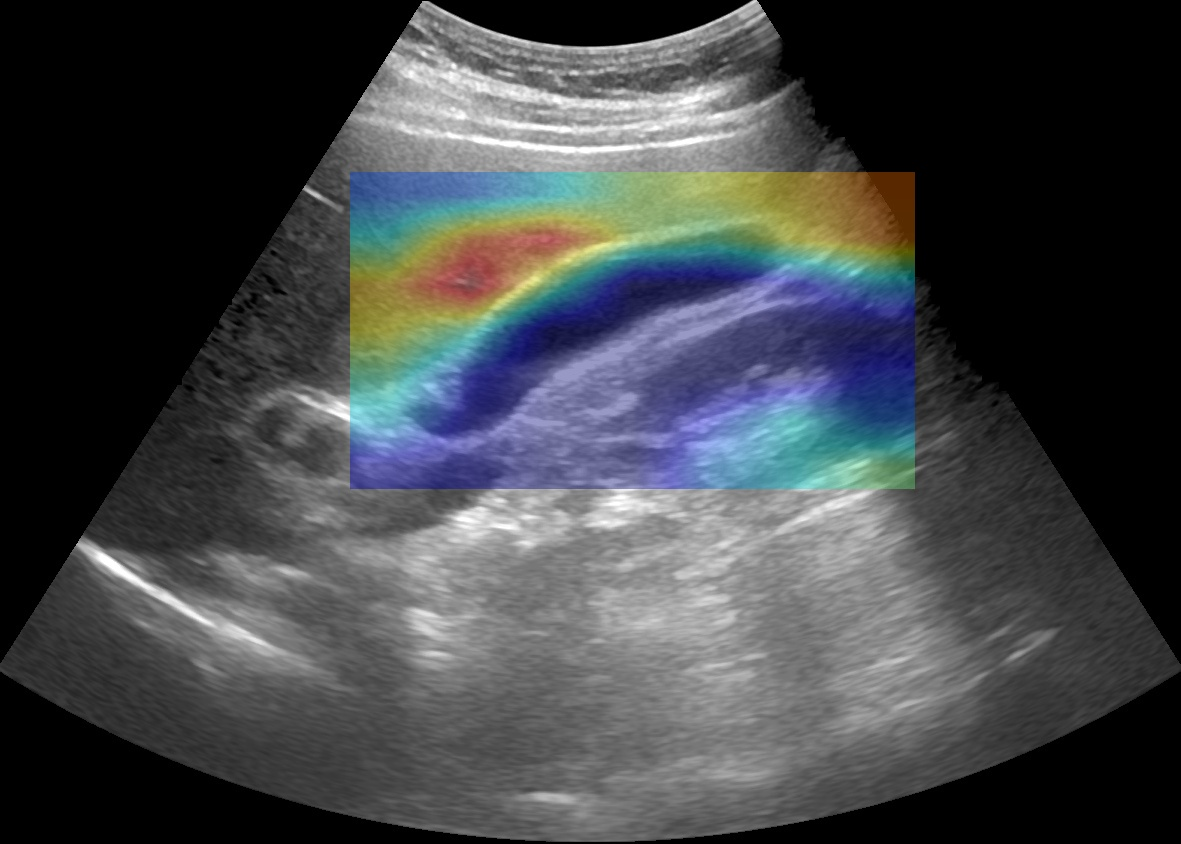
\includegraphics[width=\linewidth,height=8em]{figs/gbcnet/texture-1.jpg}
		\caption{}
		%\label{fig:multi-scale}
	\end{subfigure}
    \begin{subfigure}[b]{0.3\linewidth}
		\centering
		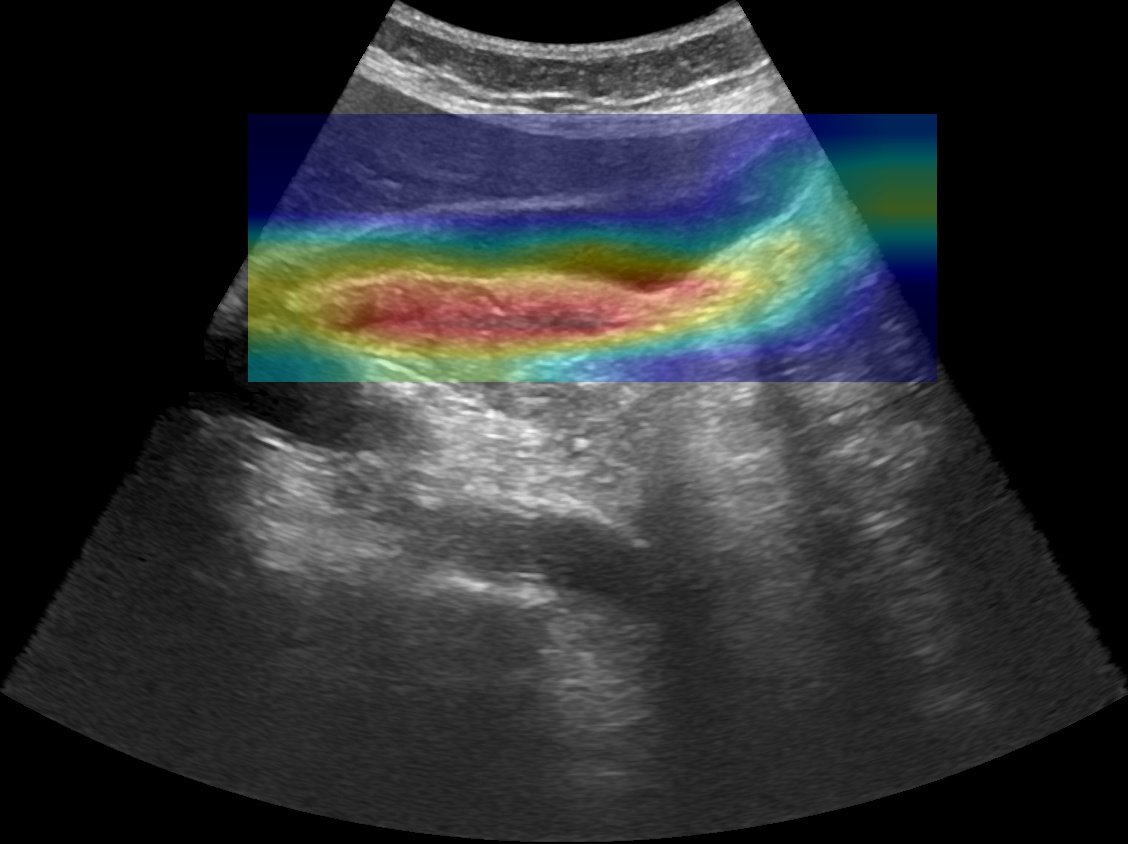
\includegraphics[width=\linewidth,height=8em]{figs/gbcnet/texture-2.jpg}
		\caption{}
		%\label{fig:multi-scale}
	\end{subfigure}
	\begin{subfigure}[b]{0.3\linewidth}
		\centering
		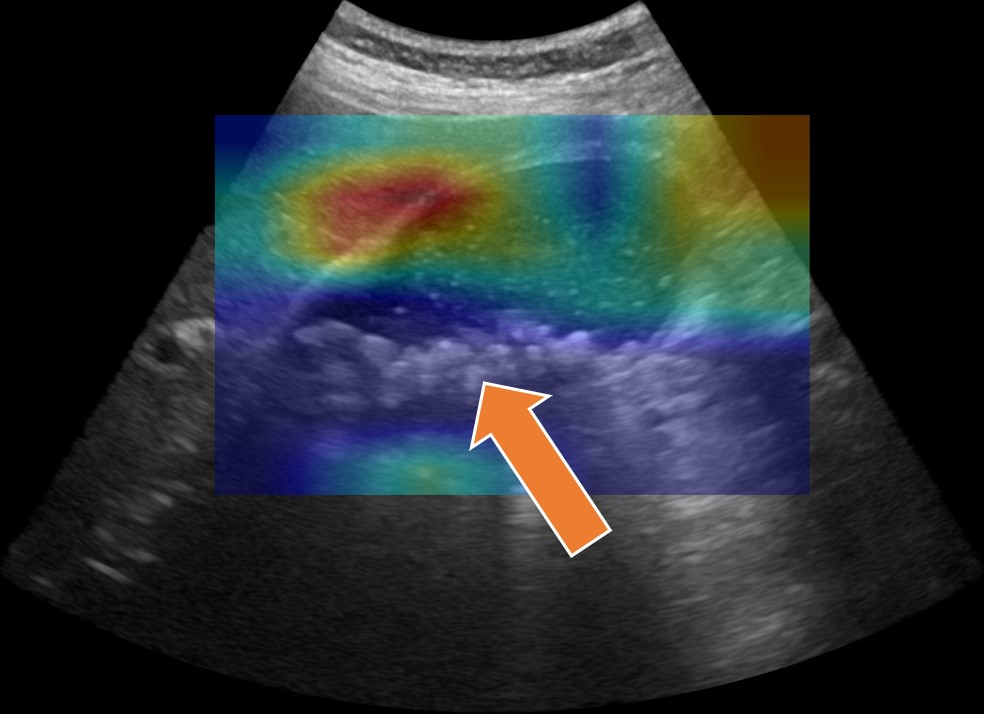
\includegraphics[width=\linewidth,height=8em]{figs/gbcnet/texture-3.jpg}
		\caption{}
		%\label{fig:multi-scale}
	\end{subfigure}
    \caption[Visualization of texture bias]{Grad-CAM visual of GBCNet trained without curriculum showing how the model tends to get biased due to the presence of textures due to noise or organ tissue. GBCNet focuses on - (a) adjacent liver tissues than the normal \gb, (b) the echogenic region below the \gb, and (c) liver textures instead of the stones (highlighted using the arrow).}
    \label{fig:texture_bias_sample}
\end{figure}
%
\begin{figure}[t]
	\centering
	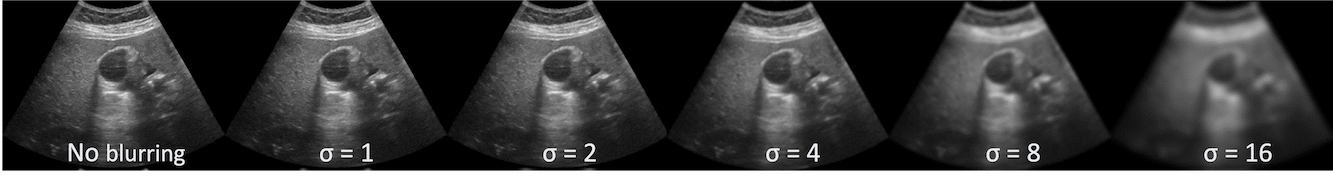
\includegraphics[width=0.95\linewidth]{figs/blur_sample_1.png}
	\caption[Gaussian blurring of USG data samples]{We simulate visual acuity through the Gaussian blur. Increasing $\sigma$ in a Gaussian filter decreases the visual acuity. Notice in the figure that, the effect of textures reduce as the visual acuity decreases and \gb shape and structure become more pronounced.}
	\label{fig:vis_acuity_sample}
\end{figure}

%% Curriculum
\subsection{Visual Acuity Inspired Curriculum}
%
We found that the textures having visual characteristics of soft tissue can adversely affect the performance of GBCNet (\cref{fig:texture_bias_sample}). We propose a curriculum to mitigate the texture bias and improve the classification. We observed that while the MS-SoP classifier is affected by texture bias, the region selection network still maintains a very high recall (\cref{tbl:perf_region}). Hence, we used the curriculum training only on the classifier and not on the region selection network.

\mypara{Visual Acuity in Humans}
%
Visual Acuity (VA) refers to the clarity and sharpness of human vision. Due to the immaturity of the retina and visual cortex, newborn children have very low VA \cite{courage1990visual}. The VA improves with the maturation of the retina and visual cortex. However, for children with congenital cataracts, the cortex matures despite the lenticular opacity. Such children begin their visual activity with higher initial VA. Evidence shows that children with high initial VA suffer to facilitate spatial analysis over expansive areas \cite{vogelsang2018VisualAcuity}.  Low VA renders blurry images that do not contain enough local information for the visual cortex to identify patterns. As a result, the visual cortex tries to increase the receptive field to facilitate spatial analysis over expansive areas and learn global features \cite{kwon2016compensation, smith2009smile}. 

\begin{algorithm}[t]
\small  
	\caption{Proposed Visual Acuity-based Curriculum}
	\label{va_algo}
	\SetAlgoLined
	\KwIn{$D^{\text{train}}$, Dataset of regions cropped from the original USG images.}
	\KwOut{Optimized model parameters $W^*$}
	Initialize $\sigma = \sigma_0$ \;
	%Set warm-up size to be $k'$ \;
	Initialize model parameters to $W$ \;
	
	\For {epoch=$\{1 \ldots, N\}$}{
		\eIf{$\sigma > 0$}{
		    $Z = \phi$ \;
    		\For {$x \in D^{\text{train}}$} {
    			$Z = Z \cup \{x \oast G(\sigma)\}$ \;
    		}
		    train($W, Z$)\;
		}
		{
		    train($W, D^{\text{train}}$) \;
		}
		\If{(epoch $> k'$) and (epoch$\%k == 0$)}{
			$\sigma = \lfloor \sigma/2 \rfloor$ \; 
		}
	}
\end{algorithm}


\mypara{Gaussian Blurring to Simulate Visual Acuity}
%
Gaussian filters are low-pass filters to cloak the high-frequency components of an input. A standard deviation $\sigma$ parameterizes the Gaussian filters. Increasing the $\sigma$ generates a higher amount of blur and low VA when convolved with an image. \cref{fig:vis_acuity_sample} shows how we can decrease the VA by increasing the $\sigma$ of a Gaussian filter. In our experiments, we have varied $\sigma$ from $1$ to $16$ to generate different levels of VA. 

\mypara{Proposed Curriculum}
%
While \cite{vogelsang2018VisualAcuity} demonstrates the improvement in receptive fields by gradually improving the sharpness of images during training, we take this observation further and show that the strategy of training on progressively higher resolution images also reduces the texture bias of a classification model. We propose a visual acuity-based training curriculum (\cref{va_algo}) that starts training the network with blurry and low-resolution \usg images and progressively increase the sharpness of training samples. The initial blurring allows the model to use an extended receptive field and focus on learning the global features such as the shape of the \gb while ignoring any noise or irrelevant textures. In the later phases, the sharp images allow the model to focus on the relevant local features in a controlled manner to make more accurate predictions. 


%\section{Dataset Collection and Curation}

\myfirstpara{Data Collection}
%
We acquired data samples from patients referred to PGIMER, Chandigarh (a tertiary care referral hospital in Northern India) for abdominal ultrasound examinations of suspected \gb pathologies. The study was approved by the Ethics Committee of PGIMER. We obtained informed written consent from the patients at the time of recruitment, and protect their privacy by fully anonymizing the data. Minimum 10 grayscale B-mode static images, including both sagittal and axial sections, were recorded by radiologists for each patient using a Logiq S8 machine. We excluded color Doppler, spectral Doppler, annotations, and measurements. Supplementary A %\ref{supp:data_collection} 
contains more details of the data acquisition process.

\mypara{Labeling and ROI Annotation}
%
Each image is labeled as one of the three classes - normal, benign, or malignant. The ground-truth labels were biopsy-proven to assert the correctness. Additionally, in each image, expert radiologists have drawn an axis-aligned bounding box spanning the entire \gb and adjacent liver parenchyma to annotate the \roi. 

\mypara{Dataset Statistics}
%
We have annotated 1255 abdominal \usg images collected from 218 patients from the acquired image corpus. Overall, we have 432 normal, 558 benign, and 265 malignant images. Of the 218 patients, 71, 100, and 47 were from the normal, benign, and malignant classes, respectively. The width of the images was between 801 and 1556 pixels, and the height was between 564 and 947 pixels due to the cropping of patient-related information. 

\mypara{Dataset Splits}
%
The sizes of the training and testing sets are 1133 and 122, respectively. To ensure generalization to unseen patients, all images of any particular patient were either in the train or the test split. The number of normal, benign, and malignant samples in the train and test set is 401, 509, 223, and 31, 49, and 42, respectively. Additionally, we report the 10-fold cross-validation metrics on the entire dataset for key experiments to assess generalization. All images of any particular patient appeared either in the training or the validation split during the cross-validation. 

%results table, pasted here for formatting reasons
%% Implementation

\section{Implementation Details}
 \begin{table}[t]
\centering
\scriptsize
%\setlength{\tabcolsep}{4pt}
    \resizebox{ \linewidth}{!}{%
        \begin{tabular}{p{0.1\linewidth}p{0.42\linewidth}p{0.06\linewidth}p{0.2\linewidth}p{0.05\linewidth}p{0.06\linewidth}}
        \toprule[1.5pt]
        \textbf{Model} & \textbf{Description} & \textbf{Input Size} & \textbf{Optimizer} & \textbf{Batch size} & \textbf{Epochs/ Steps}
        \\ \midrule[0.75pt]
        YOLOv4 \cite{yolov4} & CSPDarknet53 backbone, PANet neck, anchor-based YOLO head. Total 162-layers. Backbone was frozen for first 800 step. Entire network was trainable thereafter. Single stage, anchor-based  & $608\times608\times3$ & SGD LR = 0.0001 momentum = 0.95 weight decay = 0.0005 & 64 & 3000 steps \\ \hline
        Reppoints \cite{reppoints} & Resnet-101 backbone, Group Normalization neck, and a reppoints head. Backbone was frozen for first 30 epochs, and entire network was trainable thereafter. Two-stage, anchor-free & $800 \times 1333 \times 3$ & SGD LR = 0.001 momentum = 0.9 weight decay = 0.0001 & 4 & 50 epochs \\ \hline
        Centripetal-Net \cite{centripetalnet} & HourglassNet-104 backbone. Enitre network was trainable. Anchor-free & $511 \times 511 \times 3$ & Adam LR = 0.0005 & 4 & 50 epochs \\ \hline
        ResNet \cite{resnet} & Resnet-50 used. All layers were trainable. LR decays by 10\% after every 5 epochs through a step LR scheduler. & $224\times224\times3$ & SGD LR = 0.005 momentum = 0.9 weight decay = 0.0005 & 16 & 100 epochs \\ \hline
        VGG \cite{vgg} & VGG-16 is used. All layers were trainable. LR decays by 10\% after every 5 epochs through a step LR scheduler. & $224\times224\times3$ & SGD LR = 0.005 momentum = 0.9 weight decay = 0.0005 & 16 & 100 epochs \\ \hline
        Inception \cite{inception} & Inception-V3 used. All layers were trainable. LR decays by 10\% after every 5 epochs through a step LR scheduler. & $299\times299\times3$ & SGD LR = 0.005 momentum = 0.9 weight decay = 0.0005 & 16 & 100 epochs \\ \hline
        RetinaNet \cite{retinanet} & Resnet-18-FPN used as backbone. All layers were trainable. & $512\times512\times3$ & Adam LR = 0.0001 & 8 & 50 epochs \\ \hline
        EfficientDet \cite{efficientdet} & EfficientNet-B4 used as backbone and BiFPN as feature network. All layers were trainable. & $1024\times1024\times3$ & Adam LR = 0.001 & 2 & 50 epochs \\ 
        \bottomrule
    \end{tabular}
    }
    \caption[Implementation details for the different baseline networks]{Implementation details for the different baseline networks used for classification and \gb localization.}
    \label{tbl:configs}
\end{table}

\subsection{Transfer Learning and Data Augmentation}
%
Studies show that pre-training on natural image data improves network performance on medical image data \cite{alzubaidi2020transferlearning, cheng2017transfer}. We use \roi detection networks pre-trained on the COCO \cite{coco}, and classifiers pre-trained on ImageNet data \cite{imagenet}. We use resizing, center-cropping, and normalization data augmentations to avoid over-fitting on the small \usg dataset. We refrain from using the standard transformations like rotation or translation as they may create unrealistic images inconsistent with the ultrasound acquisition. This is also suggested in previous literature \cite{tirindelli2021rethinking}. Rotations or translation in captured ultrasound images may change the anatomical positioning information of the organs. Further, since the B-mode ultrasound captures a 2D slice of the 3D organs, rotating the probe would change the cutting plane, which is not modeled by the standard rotation transformation. 

\subsection{Hyper-parameters}
%
In the first-stage (\roi detection network) a Faster-RCNN \cite{fasterrcnn} with a Resnet-50 frozen backbone was trained using the SGD optimizer for 60 epochs with learning rate (LR) 0.005, momentum 0.9, and batch size 16. The input size was $800 \times 1333 \times 3$. In the second stage (classification), our proposed 
MS-SoP classifier was trained for 100 epochs using SGD with LR 0.005, momentum 0.9, and weight decay 0.0005. The batch size was 16. All layers of the classifier were trainable. The input images were resized to $224\times224\times3$. We train and freeze the \roi detection network before training the classifier. We used $\sigma_0\!=\!16$, $k'\!=\!10$, $k\!=\!5$, for the curriculum. We trained our models on an Nvidia Quadro P5000 16GB GPU. \cref{tbl:configs} lists the configurations of the other baseline models used during experiments. The table includes a brief description of the various stages of the network, input image sizes ($H\times W\times D$), the optimizer, and relevant hyper-parameters such as learning rate, weight decay, momentum, batch size, and the number of training epochs/steps. 


\section{Evaluation Metrics}
\label{sec:eval_metric}
%
\mypara{Localization Metrics}
%
We use mean intersection over union (mIoU), precision, and recall for comparing region selection models. IoU refers to the area of overlap (intersection) divided by the area of union between the predicted and ground truth bounding boxes. For calcutating mIoU, IoU over all samples are averaged. 
For computing precision and recall for the bounding boxes, as suggested by \cite{ribli2018detecting}, if the center of the predicted region lies within the bounding box of the ground truth region, then we consider a region prediction to be a true positive; otherwise, we consider the region prediction to be a false positive due to localization error. Further, we consider the zero/ no region prediction as a false negative (all our images contain GB, and the network's task is to merely localize it). 

\mypara{Classification Metrics}
%
To assess the classification models for \gbc detection, we use accuracy, sensitivity, and specificity as the evaluation metrics. 
\begin{align*}
    \text{Sensitivity (Recall, True Positive Rate)} &= \frac{TP}{TP+FN} \\
    \text{Specificity (True Negative Rate)} &= \frac{TN}{TN+FP} %\\
    %\text{Accuracy} &= \frac{TP+TN}{TP+TN+FP+FN}
\end{align*}
Here TP, TN, FP, and FN refer to the number of True Positives, True Negatives, False Positives, and False Negatives, respectively.



\begin{table}[t]
	\centering
	\footnotesize
	%\captionsetup{width=\textwidth}
	%\setlength{\tabcolsep}{10pt}
%	\resizebox{ \linewidth}{!}{%
		\begin{tabular}{lcccccc}
			\toprule[1pt]
			\multirow{2}{*}{\textbf{Method}} & \multicolumn{3}{c}{\textbf{Test Set}} & \multicolumn{3}{c}{\textbf{Cross Val.}} \\
			\cmidrule{2-7}
			& \textbf{Acc.} & \textbf{Spec.} & \textbf{Sens.} & \textbf{Acc.} & \textbf{Spec.} & \textbf{Sens.}  \\
			\midrule[0.5pt]
			Radiologist A & 0.816 & 0.873 & 0.707 & -- & -- & --  \\
			Radiologist B & 0.784 & 0.811 & 0.732 & -- & -- & --  \\
			\midrule
			VGG16 & 0.721 & 0.900 & 0.381 & 0.693 $\pm$ 0.036 & 0.960 $\pm$ 0.046 & 0.495 $\pm$ 0.234 \\ 
			ResNet50 & 0.787 & 0.875 & 0.619 & 0.867 $\pm$ 0.070 &  0.926 $\pm$ 0.069 & 0.672 $\pm$ 0.147 \\ 
            %0.865 +- 0.070
			Inception V3 & 0.850 & 0.875 & 0.801 & 0.844 $\pm$ 0.039 & 0.953 $\pm$ 0.029 & 0.807 $\pm$ 0.097 \\ % 0.869 $\pm$ 0.039 & 0.913 $\pm$ 0.032 & 0.708 $\pm$ 0.078 \\
			%\midrule
			Faster-RCNN & 0.779 & 0.762 & 0.810 & 0.757 $\pm$ 0.053 & 0.840 $\pm$ 0.046 & 0.808 $\pm$ 0.104 \\
			RetinaNet & 0.836 & 0.863 & 0.786 & 0.749 $\pm$ 0.073 & 0.867 $\pm$ 0.078 & 0.791 $\pm$ 0.089 \\
			EfficientDet & 0.779 & 0.863 & 0.620 & 0.739 $\pm$ 0.084 & 0.881 $\pm$ 0.099 & 0.858 $\pm$ 0.061 \\
			\midrule%[1.5pt]
			GBCNet & 0.910 & 0.900 & 0.929 & 0.882 $\pm$ 0.051 & 0.942 $\pm$ 0.037 & \textbf{0.923 $\pm$ 0.071} \\ 
			GBCNet+VA & \textbf{0.959} & \textbf{0.950} & \textbf{0.976} & \textbf{0.921 $\pm$ 0.029} & \textbf{0.967 $\pm$ 0.023} & 0.919 $\pm$ 0.063 \\
			\bottomrule[1pt]
		\end{tabular}
%	}
	\caption[Comparing GBCNet with baselines for detecting GBC from USG images]{The model performances on the test set and the cross validation (Mean$\pm$SD) in classifying \gbc from USG images. %Apart from the standard accuracy of classifying normal, benign, and malignant \gb, we show the binary classification (malignancy vs. non-malignancy) accuracy on the test set (column Acc.-2). 
    We also report the \gbc detection performance of two expert radiologists on the test set. The radiologists classified each image without accessing the biopsy results or any other patient data. Our model significantly outperforms even the human radiologists. Recall that our ground truth labels are biopsy-proven. The performance of human radiologists in the our study is comparable to that reported in literature \cite{bo2019diagnostic, gupta2020evaluation}. }
	\label{tbl:perf_gbc}
\end{table}


%
\begin{figure}[t]
	\centering
	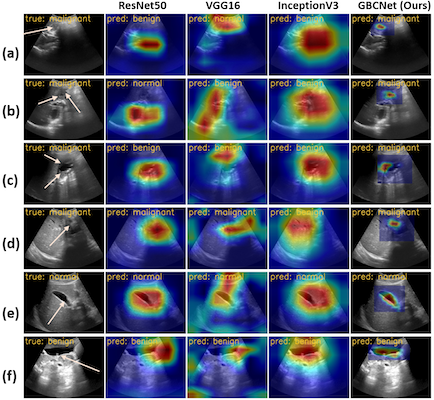
\includegraphics[width=0.62\linewidth]{figs/gbcnet/grad-cam.png}
	\caption[Qaualitative analysis of GBCNet with Grad-CAM visuals]{Grad-CAM visuals and the predictions for ResNet50, VGG16, Inception-V3, and GBCNet. The pathological areas are shown with arrows in the original images. 
	(a) ResNet50 and Inception-V3 focus on the shadow, whereas VGG16 focuses on the echogenic area, and all three fail to detect \gbc. GBCNet accurately focuses on the malignant \gb region invading the liver and detects \gbc.  (b), (c) The baseline networks focus on shadow or noise instead of the cancerous area and mispredict. 
	(d) Although ResNet50 and VGG16 predict malignancy, they fail to precisely focus on the malignant region compared to GBCNet. Inception-V3 failed to classify \gbc. (e), (f) GBCNet pinpoints the discriminating region compared to the baselines for normal and benign \gb regions, respectively. More visuals provided in \cref{fig:supple-2}.} %\ref{supp:cam_vis}.}
	\label{fig:gbc_vis}
\end{figure}

\begin{figure}[t]
	\centering
	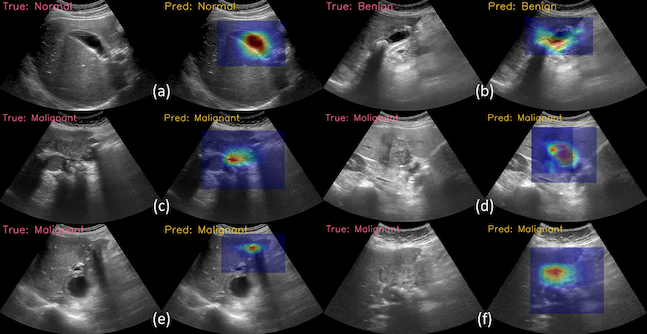
\includegraphics[width=0.7\linewidth]{figs/gbcnet/vis-s-1.png}
	\caption[Additional Grad-CAM visuals for GBCNet]{Sample Grad-CAM visuals of GBCNet with curriculum learning. (a) Normal, (b) Benign, and (c)--(f) Malignant samples.}
	\label{fig:supple-2}
\end{figure}

\section{Experiments and Results}
%
\subsection{Dataset}
%
We have used the image-based GBCU dataset described in \cref{chap:data} for the experiments. We recall that, there is a total of 1255 B-mode static abdominal USG images collected from 218 patients in this dataset. Each image is labeled as one of the three classes - normal, benign, or malignant, based on the biopsy reports. In addition to the classification labels, each image contains an axis-aligned bounding box spanning the entire \gb and adjacent liver parenchyma to annotate the \roi. The \roi in each image is drawn in consensus by two expert radiologists with 10 and 2 years of experience in abdominal radiology. The \roi (bounding box) annotations were used to train the \gb region selection network in the first stage of the GBCNet. The classification network in the second stage was trained using the image class labels. 

\mypara{Dataset Statistics}
%
Overall, we have 990 non-malignant (432 normal and 558 benign) and 265 malignant images. Of the 218 patients, 71, 100, and 47 belong to the normal, benign, and malignant classes, respectively. The width of the images was between 801 to 1556 pixels, and the height was between 564 to 947 pixels due to the cropping of patient-related information. 

\mypara{Dataset Splits}
%
The sizes of the training and testing sets are 1133 and 122, respectively. To ensure generalization to unseen patients, all images of any particular patient were either in the train or the test split. The number of normal, benign, and malignant samples in the train and test set is 401, 509, 223, and 31, 49, and 42, respectively. 
Since the dataset size is small, we also report the 10-fold cross-validation metrics on the entire dataset for key experiments to assess generalization. All images of any particular patient appeared either in the training or the validation split during the cross-validation. 

\subsection{Efficacy of GBCNet over Baselines}
%
We compare GBCNet with three popular deep classifiers, ResNet-50 \cite{resnet}, VGG-16 \cite{vgg}, and Inception-V3 \cite{inception}. We also evaluate the performance of three \sota object detectors, Faster-RCNN \cite{fasterrcnn}, RetinaNet \cite{retinanet}, and EfficientDet \cite{efficientdet} for detecting \gbc. We report the results in \cref{tbl:perf_gbc}. From the reported results, it is clear that baseline networks have poor accuracy for detecting \gbc from \usg images. Grad-CAM \cite{gradcam} visualizations in \cref{fig:gbc_vis} show that the noise, textures, and artifacts significantly influence the decision of baseline classification models. Additionally, \cref{fig:supple-2} shows the sample Grad-CAM visualizations of the predictions using GBCNet (ROI+MS-SoP) with curriculum learning. As highlighted in \cref{sec:usg_artifact_issue}, the standard DNN models tend to focus on the large shadow regions, and as a result, their classification accuracy suffers heavily. The shadow regions resembles the visual characteristics of a normal gallbladder (dark, anoechoic region). Compared to the baselines, GBCNet along-with the proposed MS-SoP classifier precisely focuses on crucial visual cues leading to its superior performance. 
%
\begin{table}[t]
	\centering
	\footnotesize
%	\captionsetup{width=\linewidth}
%    \setlength{\tabcolsep}{6pt}
%	\resizebox{\linewidth}{!}
	\caption[Comparison of the \gb region selection models]{Comparison of the \gb region selection models. We reported 10-fold cross validation (Mean$\pm$SD) of the metrics.}
\label{tbl:perf_region}
\end{table}
%
\begin{figure}[t]
	\centering
	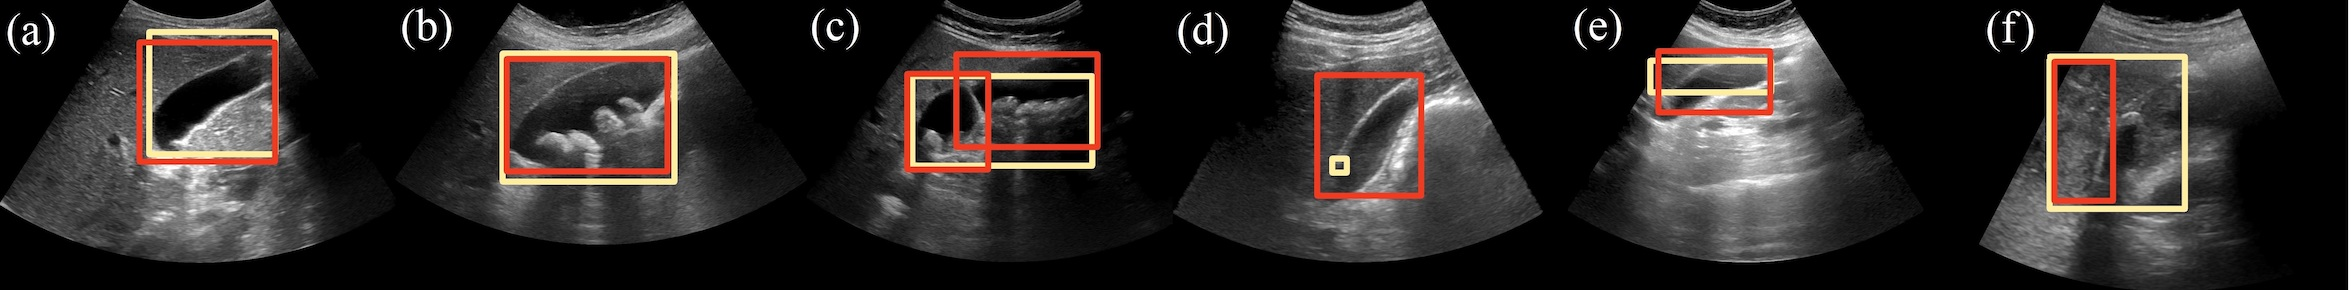
\includegraphics[width = \linewidth]{figs/roi_preds.jpg}%{figs/gbcnet/roi_preds.jpg}
	\caption[Comparison between the ROIs predicted by Faster-RCNN with radiologists]{We visually compare \roi selection by Faster-RCNN (dark red) with the \roi identified by expert Radiologists (light yellow). (a, b) The predicted a\roi matches well with the radiologists' expectations. (c) The model considers the sections partitioned by the \gb wall as separate regions. However, the union of the predicted boxes very closely approximates the actual \gb region. (d, e) Although the radiologist made an error in judging the \roi, Faster-RCNN was able to identify an accurate \roi resulting in a visually superior prediction. (f) The predicted \roi covers only a portion of the area an expert radiologist considered necessary. Even though the region prediction seems inferior compared to the human perception, expert radiologists corroborated that the predicted region captures the \gb invading the liver, a vital visual cue to detect \gbc. \roi samples from other detectors are in Appendix \cref{fig:supple-1}.}
	%\ref{supp:roi_vis}.}
	\label{fig:region_vis}
\end{figure}
%
\begin{figure}[t]
	\centering
	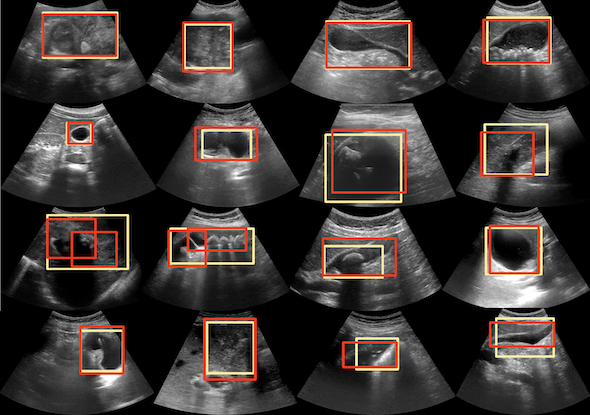
\includegraphics[width=0.7\linewidth]{figs/gbcnet/vis-s-0.png}
	\caption[Additional ROI visuals]{Sample visual results of RoI Detection models. First row - Faster-CNN, second row - YOLOv4, third row - Reppoints, and fourth row - CentripetalNet. Dark red is the ROI prediction by the model and light yellow is expert radiologists' perception of ROI.}
	\label{fig:supple-1}
\end{figure}
%
%\section{Appendix}
%
%
%\subsection{GradCAM Visuals for GBCNet}
%\label{supp:cam_vis}
Figure \ref{fig:supple-2} shows the sample Grad-CAM visualizations of the predictions using GBCNet (ROI+MS-SoP) with curriculum learning. %The blue regions show the most vital regions used by the classifier during prediction. The classifier well emphasized the crucial visual cues during inference.  

% \subsection{Candidate ROI Visuals}
% \label{supp:roi_vis}
% In figure \ref{fig:supple-1}, we show sample predictions of the GB region localization for different models. We also show the region of interest as perceived by the expert radiologists. The localization model is fairly accurate in capturing important regions of the USG image.

%
%
%\mypara{Performance of \gb Region Selection Models}
\subsection{Performance of GB Region Selection Models}
%
\cref{tbl:perf_region} summarizes the performance of various models for localizing the \gb region. For critical tasks such as region selection for cancer detection, recall is more important than precision. Multiple predicted regions can be discarded in the second stage, but missing any potentially malignant region could be disastrous. We note that the Faster-RCNN achieves the highest mIoU out of all the models while maintaining very high recall and excellent precision. Hence, we use Faster-RCNN as the region selection model. In \cref{fig:region_vis} we show the visual comparison of the \gb localization results of Faster-RCNN along with the \rois annotated by the expert radiologists. The model could predict the region of interest accurately in most cases. Although the model's prediction visually differed from the radiologists in some samples, closer inspection revealed that the predicted region retains sufficient visual cues to detect malignancy. In figure \ref{fig:supple-1}, we show additional sample predictions of the GB region localization for different models. 

\begin{table}[t]
	\centering
    \footnotesize
    \begin{tabular}{@{}lccc@{}}
    \toprule[1pt]
    \textbf{Model} & \textbf{Spec.} & \textbf{Sens.} \\
    \midrule[0.5pt]
    ResNet50 &  0.975 $\pm$ 0.024 & 0.829 $\pm$ 0.088\\
    DenseNet121  & 0.968 $\pm$ 0.018 & 0.824 $\pm$ 0.027 \\
    \midrule[0.5pt]
    MS-SoP (ours) & 0.967 $\pm$ 0.027 & 0.871 $\pm$ 0.071 \\
    \bottomrule[1pt]
    \end{tabular}
	\caption[Breast cancer detection results]{The sensitivity and specificity of MS-SoP and two baseline classifiers on breast cancer detection from USG images. We report 5-fold cross-validation on the BUSI dataset.}
\label{tbl:busi}
\end{table}

\begin{table}[t]
	\centering
	\footnotesize
	%\captionsetup{width=\linewidth}
    %\setlength{\tabcolsep}{10pt}
%    \resizebox{ \linewidth}{!}{%
    \begin{tabular}{lcccc}
    \toprule[1pt]
    \multirow{2}{*}{\textbf{Model}} & \multicolumn{2}{c}{\textbf{Orig. Test Set}} & \multicolumn{2}{c}{\textbf{Synth. Test Set}} \\
    & \textbf{Spec.} & \textbf{Sens.} & \textbf{Spec.} & \textbf{Sens.}\\
    \midrule[0.5pt]
    %AR+VGG16 & 51.6 & 56.3 & 88.1 & 55.7 ($\downarrow$) & 62.5 ($\downarrow$) & 88.1 \\
    ROI+VGG16 & 0.838 & 0.572 & 0.787 ($\downarrow$~~6.1\%) & 0.572 \\
    ROI+VGG16+VA & 0.825 & 0.762 & 0.775 ($\downarrow$~~6.1\%) & 0.762 \\
    \midrule
    %AR+ResNet50 & 84.3 & 85.7 & 88.6 & 71.3 ($\downarrow$) & 65.0 ($\downarrow$) & 88.6 \\
    %AR+ResNet50+curriculum & 91.8 & 93.8 & 97.6  & 88.5 ($\downarrow$) & 87.5 ($\downarrow$) & 97.6 \\
    ROI+ResNet50 & 0.863 & 0.857 & 0.650 ($\downarrow$24.7\%)& 0.857 \\
    ROI+ResNet50+VA & 0.938 & 0.857 & 0.887 ($\downarrow$~~5.4\%) & 0.857 \\
    \midrule
    ROI+Inception-V3 & 0.563 & 0.833 & 0.413 ($\downarrow$26.6\%) & 0.833 \\
    ROI+Inception-V3+VA & 0.913 & 0.690 & 0.788 ($\downarrow$13.7\%) & 0.690 \\
    \midrule
    GBCNet & 0.900 & 0.929 & 0.762 ($\downarrow$15.3\%) & 0.929 \\
    GBCNet+VA & 0.950 & 0.976 & 0.850 ($\downarrow$10.5\%) & 0.976 \\
    \bottomrule[1pt]
    \end{tabular}
%    }
    \caption[Robustness of the visual acuity curriculum in tacking texture bias]{Robustness of the curriculum in tacking texture bias while detecting \gbc. We show the performance of using curriculum on four models that apply classifiers on localized \gb region - (a) ROI+VGG16, (b) ROI+ResNet50, (c) ROI+Inception-V3, and (d) GBCNet (ROI+MS-SoP). The relative change (in percentage) in specificity for synthetic test data is shown within parentheses. The sensitivity remains unchanged as the malignant images were not altered. Observe that as compared to the models trained on high-resolution images, our VA-based curriculum is more robust to textures and is able to maintain a lower drop in specificity. The only exception is the ROI+VGG16 model, for which the curriculum training does not lower the drop in specificity. }
    %Also, note how the proposed curriculum is able to improve the performance of all four networks.}
\label{tbl:curr_texture}
\end{table}

\subsection{Applicability of the Proposed Classifier in Breast Cancer Detection from USG Images}
%
We explored the applicability of the proposed MS-SoP classifier on breast cancer detection from \usg images for a publicly available dataset, BUSI \cite{al2020dataset}, containing 133 normal, 487 benign, and 210 malignant images. The images in BUSI are already cropped from original \usg images to highlight only the important regions. Thus, we skip the \roi selection and run the MS-SoP classifier on BUSI. \cref{tbl:busi} shows that the MS-SoP classifier achieves much better sensitivity, which indicates the superiority of the MS-SoP architecture for malignancy identification on \usg images. We note that while breast cancer detection relies on tissue/ mass characterization, \gbc detection is primarily based on wall shape and mass anomaly. %The performance gain using MS-SoP on these two different types of cancers is interesting to note.
\par We remark that, while the MS-SoP classification network was applicable on both tasks, the Visual Acuity-based curriculum may not be suitable for Breast Cancer Detection. Breast cancer detection from USG relies heavily on the textures of the mass/ tissue in the images, as opposed to the wall shape and mass forming anomalies in GBC. Thus, while using a smoothing-based curriculum to bias the learning towards shape features is conducive for GBC detection, it may not aid breast cancer detection.

\begin{figure}[t]
	\centering
	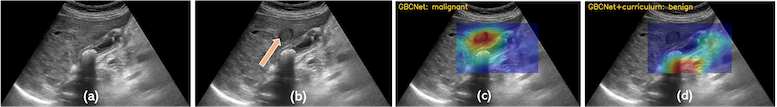
\includegraphics[width=0.9\linewidth]{figs/gbcnet/texture_vis_curr.png}
	\caption[Visualization of the effect of curriculum]{(a) Original image of a benign \gb. The \gb presents a stone and thickened wall. (b) In the synthetic image, we added an artificial tissue-like patch near the benign \gb region (highlighted by the arrow). This patch is not a part of the original \gb, and expert radiologists confirmed that the diagnosis of the \gb is not altered. (c) The textured artificial patch makes the GBCNet biased, and it focuses on the patch to predict the sample as malignant (false-positive). (d) Visual acuity curriculum fixes the texture bias of the GBCNet and helps the network to re-adjust the salient regions to the actual \gb pathology. %and learn the visual cues of a non-malignant \gb such as stone or a thickened wall.
}
	\label{fig:texture_vis}
\end{figure}

\subsection{Efficacy of the Proposed Curriculum}
%
\myfirstpara{Robustness in Tackling Texture Bias}
As described earlier, spurious textures present in \usg images tend to increase the false positives in detecting malignancy. To validate this hypothesis, we created a synthetic test set. We used the method given by \cite{yang2020fda} and added low-level frequencies from malignant images to alter the original texture of normal and benign samples. We also manually added patches looking like soft tissue near the \gb region of normal and benign images. Expert radiologists confirmed that the diagnosis of the \gb pathology is not altered. \cref{tbl:curr_texture} shows that the specificity decreases due to the increase of the false positives. The sensitivity remains unaffected as the prediction for malignant \gb samples was unchanged. The network trained with the proposed curriculum tackles texture bias well and accurately predicts non-malignant samples in synthetic test data. This experiment shows that the proposed curriculum effectively tackles texture bias. \cref{fig:texture_vis} shows a visual sample of how the soft tissue-like texture influences the network's decision and how the curriculum helps the network to rectify the discriminative regions. 

\begin{table}[t]
	\centering
	\footnotesize
%	\captionsetup{width=\linewidth}
%    \setlength{\tabcolsep}{6pt}
%	\resizebox{\linewidth}{!}{%
    \begin{tabular}{@{}lccc@{}}
    \toprule[1pt]
    \textbf{Model} & \textbf{Acc} & \textbf{Spec.} & \textbf{Sens.} \\
    \midrule[0.5pt]
    ROI+VGG16 & 0.533 $\pm$ 0.092 & 0.719 $\pm$ 0.115 & 0.733 $\pm$ 0.179\\
    ROI+VGG16+VA & 0.777 $\pm$ 0.041 & 0.938 $\pm$ 0.030 & 72.0 $\pm$ 0.195\\
    \midrule
    ROI+ResNet50 & 0.766 $\pm$ 0.107 &  0.823 $\pm$ 0.105 & 0.909 $\pm$ 0.111\\
    ROI+ResNet50+VA & 0.854 $\pm$ 0.077 & 0.923 $\pm$ 0.059 & 0.875 $\pm$ 0.091 \\
    \midrule
    ROI+Inception-V3 & 0.718 $\pm$ 0.089 & 0.833 $\pm$ 0.087 & 0.785 $\pm$ 0.214\\
    ROI+Inception-V3+VA & 0.826 $\pm$ 0.046 & 0.931 $\pm$ 0.044 & 0.826 $\pm$ 0.099\\
    \midrule
    % RetinaNet & 74.9 $\pm$ 7.3 &  86.7 $\pm$ 7.8 & 79.1 $\pm$ 8.9\\
    % RetinaNet+VA & 73.3 $\pm$ 6.0 & 92.1 $\pm$ 4.4 & 70.6 $\pm$ 14.2\\
    % \midrule
    GBCNet (ROI+MS-SoP) & 0.882 $\pm$ 0.051 & 0.942 $\pm$ 0.037 & 0.923 $\pm$ 0.071\\
    GBCNet+VA & 0.921 $\pm$ 0.029 &  0.967 $\pm$ 0.023 & 0.919 $\pm$ 0.063\\
    \bottomrule[1pt]
    \end{tabular}
%	}
	\caption[Model performances for training with visual acuity curriculum]{Model performances (10-fold cross-validation) for training with our proposed visual acuity-based curriculum.}
\label{tbl:curr_improve}
\end{table}

\mypara{Performance Improvement with Proposed Curriculum}
We also assess the quantitative performance improvement of models due to the curriculum training in \cref{tbl:curr_improve}. All models show improvement in specificity, which indicates the effectiveness of the proposed blurring-based curriculum in tackling texture bias, and reducing false positives. 

%\subsubsection{Generalization to multiple resolutions}
%%
%To verify how well can the curriculum enhance the generalization capability of \GBCNet at different resolutions, we evaluate the performance of the \GBCNet on the test set at different resolutions. We do this by blurring the test set using different values of $\sigma$ and evaluating GBCNet on these images. Like before, we evaluated the GBCNet without any curriculum and GBCNet with curriculum, anti-curriculum, and the control-curriculum models. The results of this comparison can be seen in \cref{fig:gbc_curr_blur}. The model trained using our proposed curriculum generalizes well across a larger spectrum of image resolutions, and this is an indicator of better spatial understanding than the other models. Note that, the blurred images improve the detection of non-malignant test samples (\cref{fig:spec-test-blur}) for all models. This is an alternate validation of the hypothesis that non-malignant samples (normal and benign) learn better from shape than textures. An interesting observation is that the anti-curriculum performs well at highly blurred (low-resolution) test samples. This can be explained from the fact that anti-curriculum is presented with low-resolution images towards the end of the training cycle. Thus, it maintains the sensitivity better for low-resolution test samples. The curriculum-based GBCNet learns high resolution images towards the later part of the training and thus the sensitivity starts to degrade with low resolution images.

\begin{figure}[t]
	\centering
	\begin{subfigure}[b]{0.23\linewidth}
    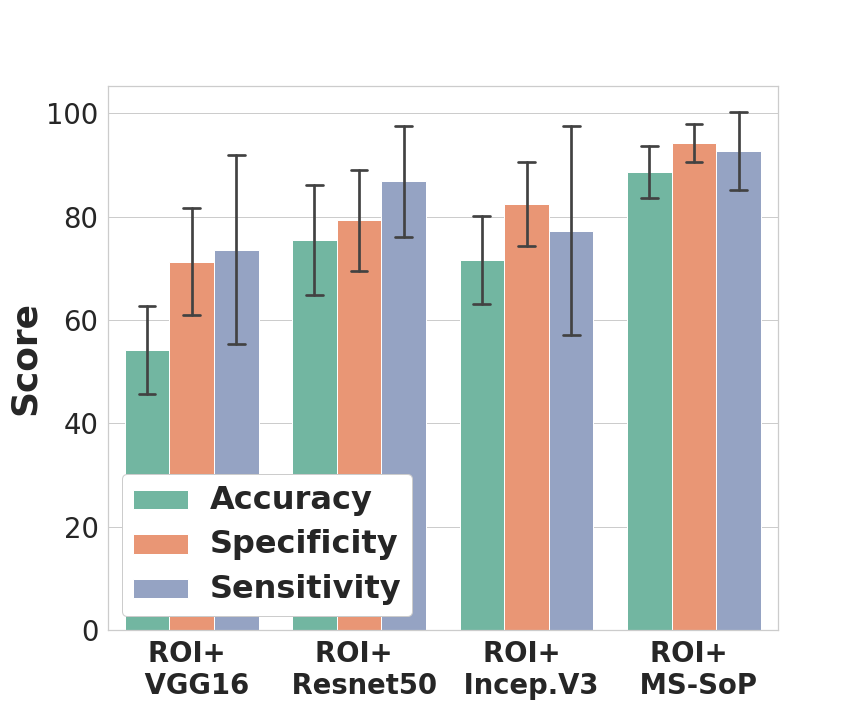
\includegraphics[width=\linewidth]{figs/gbcnet/roi_models.png}
    \caption{}
    \label{fig:perf_attn_models}
    \end{subfigure}
	\begin{subfigure}[b]{0.23\linewidth}
		\centering
		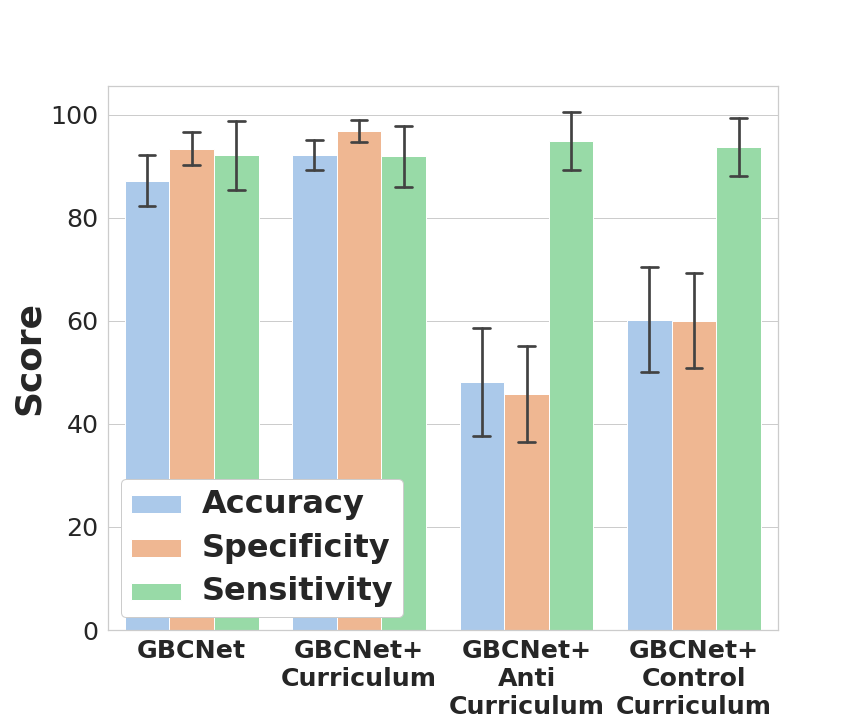
\includegraphics[width=\linewidth]{figs/gbcnet/curr_pred.png}
		\caption{}
		\label{fig:ablation1}
	\end{subfigure}
	%
	\begin{subfigure}[b]{0.23\linewidth}
		\centering
		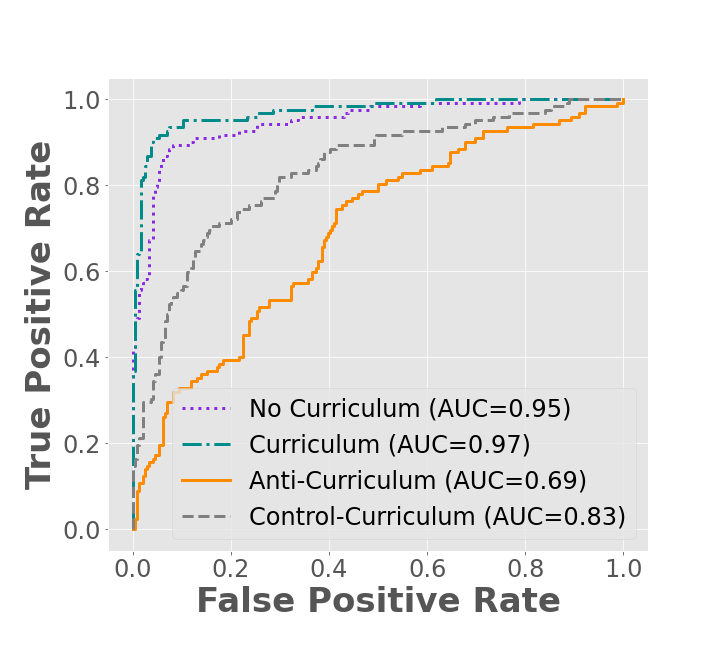
\includegraphics[width=\linewidth]{figs/gbcnet/roc.png}
		\caption{}
		\label{fig:ablation2}
	\end{subfigure}
		\begin{subfigure}[b]{0.23\linewidth}
		\centering
		\includegraphics[width=\linewidth]{figs/gbcnet/acc-mr.png}
		\caption{}
		\label{fig:ablation3}
	\end{subfigure}
	\caption[Ablation study]{Ablation study. (a) Comparison of accuracy, specificity, and sensitivity for applying different classification networks (VGG16, ResNet50, Inception-V3, and MS-SoP) on the localized \gb. We have reported the 10-fold cross validation results. (b) The efficacy of the proposed training regime in terms of accuracy, specificity, sensitivity. (c) ROC-AUC for different training regimes on the test set. (d) The proposed curriculum generalizes better at different resolutions. }
	\label{fig:diff_images}
\end{figure}

\subsection{Ablation Study}
%
\myfirstpara{Choice of Classifier in GBCNet}
%
We have plugged in other deep classification networks in place of the proposed MS-SoP classifier in the GBCNet framework. \cref{fig:perf_attn_models} summarizes the results. The MS-SoP classifier on GBCNet provides the best \gbc detection accuracy. Using the classifiers on the \rois improves the sensitivity and accuracy for ResNet50 and VGG16. However, the drop in specificity results in performance degradation for Inception-V3 as the sensitivity was not improved.  

\mypara{Choice of Training Regime}
%
We used the proposed GBCNet model to assess the influence of the visual acuity-based curriculum. We compare the curriculum with two possible alternatives - (i) \emph{anti-curriculum} that initially trains with high resolution and progressively lowers the resolution, and (ii) \emph{control-curriculum} where the samples are not sorted resolution-wise, and the curriculum contains a random set of blurred samples. Note that the control-curriculum can also be thought of using Gaussian blurring as a data augmentation where the probability of choosing a particular $\sigma$ is equal to the fraction of epochs the $\sigma$ used during the curriculum. \cref{fig:ablation1} and \ref{fig:ablation2} show the performance of the various curriculum strategies on the performance on GBCNet.  %\cref{fig:gbc_curr_blur} shows the ROC with the AUC for GBCNet with different curriculum. 
%Additionally, \cref{tbl:curr_texture} shows the performance improvement of attention region-based classifiers when trained with the proposed curriculum.
Further, to understand how various curriculum strategies affect a model's generalization at different resolutions, we blur the test set using different values of $\sigma$ and evaluate the models on these images (\cref{fig:ablation3}). 
%The results of this comparison can be seen in \cref{fig:ablation3}. 
We see that the model trained using the proposed curriculum generalizes well across different image resolutions, which is an indicator of better spatial understanding.

\begin{table}[t]
	\centering
	\footnotesize
%	\captionsetup{width=\linewidth}
%    \setlength{\tabcolsep}{6pt}
%	\resizebox{\linewidth}{!}{%
    \begin{tabular}{@{}lccc@{}}
    \toprule[1pt]
    \textbf{Model} & \textbf{Spec.} & \textbf{Sens.} \\
    \midrule[0.5pt]
    ROI+MS-SoP (GBCNet) & 0.942 $\pm$ 0.037 & 0.923 $\pm$ 0.071 \\
    ROI+MS-SoP (channel-wise pooling) & 0.904 $\pm$ 0.047 & 0.861 $\pm$ 0.068  \\
    ROI+MS-SoP (spatial pooling) & 0.900 $\pm$ 0.064 & 0.882 $\pm$ 0.064 \\
    ROI+MS (w/o SoP) & 0.887 $\pm$ 0.060 & 0.872 $\pm$ 0.064 \\
    ROI+SoP (w/o MS) & 0.914 $\pm$ 0.048 & 0.854 $\pm$ 0.079 \\
    \bottomrule[1pt]
    \end{tabular}
%	}
	\caption[Ablation of the proposed MS-SoP network]{Ablation of Ms-SoP. We show the specificity and sensitivity of MS-SoP with two alternatives - MS-SoP with (i) only channel-wise and (ii) only spatial pooling. We also show the efficacy of using multi-scale and second-order pooling in conjunction.}
\label{tbl:ms-sop-ablation}
\end{table}

\mypara{Components of the MS-SoP Classifier}
%
We present the ablation study on the MS-SoP classifier in \cref{tbl:ms-sop-ablation}. We show the effect of the multi-scale and second-order pooling components on the specificity and sensitivity of the model. We also show the relevance of the channel-wise and spatial pooling in the second-order pooling.
\section{Conclusion}
%\todo{We have observed that our proposed system fails to capture the inaccuracies caused by the small mass or irregular structures near the gallbladder wall. Since gallbladder is a hollow organ, the malignancy starts from the wall. For nearly 5\% of the images, the irregularity and minuscule structures of the wall needs discerning between the noise, soft tissue texture, and the tiny wall structure.} 
In this chapter, we addressed Gallbladder Cancer detection from USG images using deep learning and proposed a new supervised learning framework (GBCNet) based on \roi selection and a multi-scale second-order pooling. The proposed design helps the classifier focus on the crucial \gb region predicted by the region selection network, and make better predictions by mitigating the effect of noise and artifacts. We also tested the performance of the proposed MS-SoP classifier on breast cancer detection from USG. The performance gain using MS-SoP on these two different types of cancers indicates that the model is capable of learning robust representations of different types of malignancy in USG images. We also proposed a visual acuity-based curriculum to make our design resilient to texture bias and improve its specificity of GBCNet. Extensive experiments show that GBCNet, combined with the curriculum learning, improves performance over the baseline deep classification and object detection architectures. Our work tackles the impediments posed by \usg images towards making accurate GBC detection, an important but hitherto overlooked problem.
%In the future, we would like to explore if the proposed network architecture and the visual acuity-based curriculum can help improve predictions in other cancer detection problems.
%We chose breast cancer detection, a prominent problem in this domain, and validated the MS-SoP classifier on the public breast ultrasound image (BUSI) dataset. We note that while breast cancer detection relies on tissue/ mass characterization, GBC detection is primarily based on wall shape and mass anomaly. The performance gain using MS-SoP on these two different types of cancers indicates efficient malignancy representation by our model. We plan to evaluate our method on other datasets as future work to formally understand the efficacy and the characterization of malignancy representation by MS-SoP for different types of cancers.

%{\small \mypara{Acknowledgement} The authors thank IIT Delhi HPC facility for computational resources.}
%\begin{figure}[t]
	\centering
	\includegraphics[width=0.7\linewidth]{figs/gbcnet/vis-s-1.png}
	\caption[Additional Grad-CAM visuals for GBCNet]{Sample Grad-CAM visuals of GBCNet with curriculum learning. (a) Normal, (b) Benign, and (c)--(f) Malignant samples.}
	\label{fig:supple-2}
\end{figure}

\begin{figure}[t]
	\centering
	\includegraphics[width=0.7\linewidth]{figs/gbcnet/vis-s-0.png}
	\caption[Additional ROI visuals]{Sample visual results of RoI Detection models. First row - Faster-CNN, second row - YOLOv4, third row - Reppoints, and fourth row - CentripetalNet. Dark red is the ROI prediction by the model and light yellow is expert radiologists' perception of ROI.}
	\label{fig:supple-1}
\end{figure}

\section{Appendix}


\subsection{GradCAM Visuals for GBCNet}
\label{supp:cam_vis}
Figure \ref{fig:supple-2} shows the sample Grad-CAM visualizations of the predictions using GBCNet (ROI+MS-SoP) with curriculum learning. %The blue regions show the most vital regions used by the classifier during prediction. The classifier well emphasized the crucial visual cues during inference.  

\subsection{Candidate ROI Visuals}
\label{supp:roi_vis}
In figure \ref{fig:supple-1}, we show sample predictions of the GB region localization for different models. We also show the region of interest as perceived by the expert radiologists. The localization model is fairly accurate in capturing important regions of the USG image.

\subsection{Baseline Implementation Details}
%

\label{supp:impl}
\cref{tbl:configs} lists the configurations of all models which we have used. We trained on the Quadro P5000 16GB GPU. The table includes a brief description of the various stages of the network, input image sizes ($H\times W\times D$), the optimizer, relevant hyper-parameters such as learning rate, weight decay, momentum, batch size, and the number of training epochs/steps for the network. 
 \begin{table}[t]
\centering
\footnotesize
%\setlength{\tabcolsep}{4pt}
    \resizebox{ \linewidth}{!}{%
        \begin{tabular}{p{0.1\linewidth}p{0.42\linewidth}p{0.06\linewidth}p{0.2\linewidth}p{0.05\linewidth}p{0.06\linewidth}}
        \toprule[1.5pt]
        \textbf{Model} & \textbf{Description} & \textbf{Input Size} & \textbf{Optimizer} & \textbf{Batch size} & \textbf{Epochs/ Steps}
        \\ \midrule[0.75pt]
        YOLOv4 \cite{yolov4} & CSPDarknet53 backbone, PANet neck, anchor-based YOLO head. Total 162-layers. Backbone was frozen for first 800 step. Entire network was trainable thereafter. Single stage, anchor-based  & $608\times608\times3$ & SGD LR = 0.0001 momentum = 0.95 weight decay = 0.0005 & 64 & 3000 steps \\ \hline
        Reppoints \cite{reppoints} & Resnet-101 backbone, Group Normalization neck, and a reppoints head. Backbone was frozen for first 30 epochs, and entire network was trainable thereafter. Two-stage, anchor-free & $800 \times 1333 \times 3$ & SGD LR = 0.001 momentum = 0.9 weight decay = 0.0001 & 4 & 50 epochs \\ \hline
        Centripetal-Net \cite{centripetalnet} & HourglassNet-104 backbone. Enitre network was trainable. Anchor-free & $511 \times 511 \times 3$ & Adam LR = 0.0005 & 4 & 50 epochs \\ \hline
        ResNet \cite{resnet} & Resnet-50 used. All layers were trainable. LR decays by 10\% after every 5 epochs through a step LR scheduler. & $224\times224\times3$ & SGD LR = 0.005 momentum = 0.9 weight decay = 0.0005 & 16 & 100 epochs \\ \hline
        VGG \cite{vgg} & VGG-16 is used. All layers were trainable. LR decays by 10\% after every 5 epochs through a step LR scheduler. & $224\times224\times3$ & SGD LR = 0.005 momentum = 0.9 weight decay = 0.0005 & 16 & 100 epochs \\ \hline
        Inception \cite{inception} & Inception-V3 used. All layers were trainable. LR decays by 10\% after every 5 epochs through a step LR scheduler. & $299\times299\times3$ & SGD LR = 0.005 momentum = 0.9 weight decay = 0.0005 & 16 & 100 epochs \\ \hline
        RetinaNet \cite{retinanet} & Resnet-18-FPN used as backbone. All layers were trainable. & $512\times512\times3$ & Adam LR = 0.0001 & 8 & 50 epochs \\ \hline
        EfficientDet \cite{efficientdet} & EfficientNet-B4 used as backbone and BiFPN as feature network. All layers were trainable. & $1024\times1024\times3$ & Adam LR = 0.001 & 2 & 50 epochs \\ 
        \bottomrule
    \end{tabular}
    }
    \caption[Implementation details for the different baseline networks]{Implementation details for the different baseline networks used for classification and \gb localization.}
    \label{tbl:configs}
\end{table}








\chapter{Learning from Limited Supervised Data I: Using Unlabelled Videos}
\label{chap:limited}
Previously, we have developed \gbcnet to tackle the issues in USG images and achieved superior GBC detection performance compared to the state-of-the-art CNN models, and expert radiologists. However, the reliance on bounding box annotations to train the ROI detection phase in \gbcnet poses a bottleneck. Medical data annotation requires trained medical experts. The cost of obtaining annotations is thus very high due to the complexity and involvement of trained experts. Such annotation also adds additional burden on the medical professionals as they already face time constraints due to high patient influx. In this chapter, we tackle a key challenge associated with medical image computing and analysis -- paucity of annotated dataset, and explore the utilization of limited supervised data for training deep neural networks (DNNs) to detect GBC from USG images. In this chapter, 
%We investigate two distinct approaches towards this direction -- (1) 
we introduce an unsupervised contrastive framework designed to leverage unlabelled video data for effective representation learning, ultimately benefiting downstream GBC detection from USG images.%, and (2) we use a weakly supervised object detection technique to detect GBC with only image-level labels instead of the costly bounding box annotations during training. 
The contents in this chapter are based on the following published work:
\par \noindent [1] \textit{Soumen Basu, Somanshu Singla, Mayank Gupta, Pratyaksha Rana, Pankaj Gupta, and Chetan Arora.
``Unsupervised Contrastive Learning of Image Representations from Ultrasound Videos with Hard Negative Mining.'' International Conference on Medical Image Computing and Computer-Assisted Intervention (MICCAI). 2022}. 

%\section{Representation Learning with Unlabelled Video Data}
\label{chap:usucl}

%Rich temporal information and variations in viewpoints make video data an attractive choice for learning image representations using unsupervised contrastive learning (UCL) techniques. State-of-the-art (SOTA) contrastive learning techniques consider frames within a video as positives in the embedding space, whereas the frames from other videos are considered negatives. We observe that unlike multiple views of an object in natural scene videos, an USG video captures different 2D slices of an organ. Hence, there is almost no similarity between the temporally distant frames of even the same USG video. In this paper we propose to instead utilize such frames as hard negatives. We advocate mining both intra-video and cross-video negatives in a hardness-sensitive negative mining curriculum in a UCL framework to learn rich image representations. We deploy our framework to learn the representations of Gallbladder (GB) malignancy from USG videos. We also construct the first large-scale USG video dataset containing 64 videos and 15,800 frames for learning GB representations. We show that the standard ResNet50 backbone trained with our framework improves the accuracy of models pretrained with SOTA UCL techniques as well as supervised pretrained models on ImageNet for the GB malignancy detection task by 2--6\%. We further validate the generalizability of our method on a publicly available lung USG image dataset of COVID-19 pathologies and show an improvement of 1.5\% compared to SOTA. Source code, dataset, and models are available at \url{https://gbc-iitd.github.io/usucl}.
	
% \keywords{Contrastive Learning \and Ultrasound \and Negative Mining}
% \end{abstract}

% ---- Introduction ----
%
\section{Introduction}

%Due to their remarkable performance, Deep Neural Networks (DNNs) have become defacto standard for a wide range of medical image analysis tasks in recent years \cite{ardila2019end,bejnordi2017diagnostic}. However, 
Lack of annotated medical data due to the specialized nature of annotations, and the data privacy issues restrict the applicability of supervised learning of DNNs in medical imaging. Although pretraining on large natural image datasets yields a performance boost for downstream tasks on medical data \cite{alzubaidi2020transferlearning,cheng2017transfer}, the large domain gap between the natural and medical images remains a bottleneck. Recent works are increasingly going beyond the supervised setup and exploiting unsupervised techniques to compensate for the lack of annotated data \cite{simclr,moco}. Broadly, there are two prominent categories of representation learning techniques for leveraging unlabeled data. In the pretext task-based method, the DNNs are pretrained with some spatial tasks such as image rotation prediction \cite{komodakis2018unsupervised} or temporal tasks such as video clip order prediction \cite{xu2019self} to learn efficient image representation. On the other hand, contrastive methods \cite{simclr} try to distinguish between different views of image samples to learn robust representation without labels. Visual representations learned by contrastive learning have been shown to outperform the supervised pretraining on large annotated data in terms of accuracy on the downstream prediction tasks \cite{simclr,moco}.  

\begin{figure}[t]
    \centering
    \includegraphics[width=\linewidth]{figs/usucl/teaser.png}
    \caption[Motivation of using intra-video negatives]{We motivate the use of intra-video negatives in contrastive learning. Based on the visibility of a pathology in the intra-video samples, negatives can be sampled. The frames in range $[T-\delta, T+\delta]$ in video $V^i$ has stones and malignant wall thickening visible for a small $\delta$. A slightly distant frame $T+t_1$ shows a GB, but the malignant wall thickening is not visible. This sample acts as a hard negative. The viewing plane further changes in frame $T+t_2$ and GB becomes invisible.}
    \label{usucl_fig:teaser}
\end{figure}

Video data contains rich variations in viewpoints and natural temporal information for objects making it suitable for going beyond image-level contrastive learning. Additionally, the abundance of unlabeled video data makes it an attractive choice for learning representations. Recent works are attempting to exploit the video data to learn robust image-level representations \cite{uscl,cyclecontrast}. We observe that current SOTA techniques for image representation learning from videos, such as USCL \cite{uscl} suggest that images coming from the same video are too close to be considered negatives (\emph{similarity conflict}). USCL advocates considering only cross-video samples as negatives to avoid the similarity conflict. While similarity conflict is prevalent for intra-video samples of natural video datasets like action recognition, where each video contains a distinct action, the USG videos are inherently different. We observe that unlike multiple views of an object in natural scene videos, an USG video captures different 2D slices of an organ. Hence, there is almost no similarity between the temporally distant frames of even the same USG video. We propose to instead utilize such frames as negatives. The frames of a USG video contain both types of images where pathology maybe visible or absent. \cref{usucl_fig:teaser} shows the positive and negative frames from the same USG video. The temporal distance between the frames acts as a proxy to the hardness. Negative samples that are temporally closer to the positives contain higher similarities with the positives and are harder to differentiate in the embedding space. We propose an unsupervised contrastive framework to exploit both the intra-video and cross-video negatives for learning robust visual representations from USG videos. We design a hardness-sensitive negative mining curriculum to lower the distance between the anchor and negatives gradually. Due to its unsupervised nature, our technique can be used for pretraining a backbone on any USG video dataset for superior downstream performance.

We deploy our video contrastive learning framework to pretrain a neural network before supervised fine-tuning to identify GBC in USG images. 
%Due to its non-ionizing radiation, low cost, and accessibility, USG is a popular non-invasive diagnostic modality for patients with suspected GB pathology. Although there are prior works involving DNNs to detect GB afflictions such as polyp or stones \cite{gbPolyp,gbPolyp2,gbAutomatic}, there is limited prior work on using DNNs to detect GB malignancy in USG images \cite{basu2022surpassing}. 
Unlike detecting stones or polyps, identifying GB malignancy from the routine USG is challenging for radiologists \cite{gb-rads-paper,gupta2020imaging}. We observed that ImageNet pretrained classifiers perform even worse than radiologists. 
%We used an USG video dataset to pretrain our model. 
Our contrastive learning-based pretraining on USG videos help the model to surpass human radiologists and SOTA contrastive learning methods on GBC classification.

We also validate the generality our framework on a public lung USG dataset, POCUS \cite{pocus}, containing COVID-19 and Pneumonia samples. Pretraining our model on public lung USG videos, and finetuning for the downstream classification shows improvement over ImageNet pretraining and the current SOTA contrastive techniques.

% \mypara{Contributions} Our key contributions in this chapter are:
% \begin{itemize}
% \itemsep0em
% 	\item  We design an unsupervised contrastive learning technique for USG videos to exploit both cross-video and intra-video negatives for rich representation learning. We further use a hardness-sensitive negative mining curriculum to boost the performance of our contrastive learning framework.
% 	%
% 	\item We deploy our framework to solve a novel GB malignancy classification problem from USG images. We also validate the efficacy of our technique on a publicly available lung USG dataset for COVID detection.
% 	%
% 	%\item We are contributing the first USG video dataset of 64 videos and 15800 frames containing both malignant and non-malignant GB towards the development of representation learning from medical USG videos.
% \end{itemize}

% ---- Dataset ----
%
\begin{figure}[t]
    \centering
    \includegraphics[width=0.9\linewidth]{figs/usucl/data_sample.png}
    \caption[Sample video sequences for the GBC and Covid Ultrasound data]{Sample video sequences from the GB USG video and the Butterfly \cite{butterfly} datasets. Two sequences of size 4 is shown on the left and right for each dataset.}
    \label{usucl_fig:data_sample}
\end{figure}
%
\section{Data}
%
\subsection{USG Dataset for Gallbladder Cancer}
%
We have used the GBUSV dataset described in \cref{data:gbusv} for the unsupervised contrastive pretraining, and the GBCU dataset (\cref{data:gbcu}) for the downstream GBC classification task. For helping the reader, we briefly describe the data in this section as well.

\mypara{Video Data for Contrastive Pretraining}
%
Radiologists with 2-8 years of experience in abdominal sonography acquired the data. The USG videos were obtained after at least 6 hours of fasting using a 1--5 MHz curved array transducer (C-1-5D, Logiq S8, GE Healthcare). The scanning intended to include the entire GB and the lesion or pathology. %The frame rate was 29 fps. 
The length of the videos varied from 43 to 888 frames. %depending on the GB distension and size of the lesion. 
The dataset consists of 32 malignant and 32 non-malignant videos containing a total of 12,251 and 3,549 frames, respectively. We do not use the video level labels in the contrastive pretraining. We cropped the video frames from the center to anonymize the patient information. The processed video frames were of size $360\!\times\!480$ pixels. \cref{usucl_fig:data_sample} shows some samples from the video data. 

\mypara{Image Data for Downstream GBC Classification}
%
GBCU dataset \cite{basu2022surpassing} consists of 1255 USG images from 218 patients. The images were labeled as normal, benign, or malignant, and such labels were biopsy-proven. The dataset consists of 990 non-malignant (432 normal, 558 benign) and 265 malignant images.  We use this dataset for finetuning and report 10-fold cross-validation. We did the cross-validation splits at the patient level. 
The patients recorded in the video dataset are different from the patients used in the image dataset to ensure generalization. 

\subsection{Public Lung USG Dataset for COVID-19}

\myfirstpara{Video Data}
%
We use the public lung USG video dataset, Butterfly \cite{butterfly}. Butterfly consists of 22 USG videos containing 1533 images of size $658\!\times\!758$ pixels of the lung. The dataset was collected using a Resona 7T machine.

\mypara{Image Data}
%
We use the publicly available POCUS \cite{pocus} dataset consisting of a total of 2116 lung USG images, of which 655, 349, and 1112 images are of COVID-19, bacterial pneumonia, and healthy control, respectively.

%
% ---- Methods ----
%
\section{Methodology}

\begin{figure}[t]
    \centering
    \includegraphics[width=0.9\linewidth]{figs/usucl/arch1.png}
    \caption[Overview of the proposed contrastive framework]{Overview of the proposed contrastive loss, $\mathcal{L}$. An anchor $\vb{q}$ and another temporally close sample $\vb{z}^+$ from the same video are used as positive pairs. Given the set of cross-video negatives $N$, and the intra-video negatives $\vb{z}_j^-$, we compute $\vb{\hat{z}}^-$ from the $m$ most similar cross-video negatives to the anchor. The intra-video samples $\vb{z}_j^-$ and $\vb{\hat{z}}^-$ are considered as negatives to the anchor.}
    \label{usucl_fig:my_label}
\end{figure}

\mypara{Contrastive Learning Setup}
%
Suppose, $\vb{V}^i = \big\{ \vb{x}_j\big\}_{j=1}^{M^i}$ is the $i$-th video in the video dataset consisting of $M^i$ frames where $\vb{x}_j$ is the $j$-th individual frame. We sample an anchor image, $\vb{x}_a$, a positive image $\vb{x}_p$, and $k$ negative frames $\vb{x}_{n_1}, \ldots, \vb{x}_{n_k}$ from a video using a sampler $\vb{\Theta}$. We encode the samples using a backbone $f$ followed by a two layer MLP, $g$ that creates a 128 dimensional embedding vector. We denote the embedding vectors as:
%
\begin{align}
    \vb{q} = g(f(\vb{x}_a)), \qquad
    \vb{z}^+ = g(f(\vb{x}_p)), ~ \text{and} \qquad
    \vb{z}_j^- = g(f(\vb{x}_{n_j})).
\end{align}
%
We maximize the agreement between (positive, anchor) and minimize between (anchor, negatives) pairs in the embedding space. Let $N$ be the set of cross video negatives generated from other videos in the dataset. To exploit the cross-video negatives, we calculate the normalized similarity measure between $\vb{q}$ and $\vb{z}$ for all $\vb{z} \in N$:
%
\begin{align}
    \alpha_{\vb{q},\vb{z}}= \frac{\exp\big(s(\vb{q}, \vb{z})/\tau\big)}{ \sum_{\vb{z}_c\in N}\exp\big(s(\vb{q}, \vb{z}_c)/\tau\big)},
\end{align}
%
where $s(\vb{a}, \vb{b}) = \vb{a}\cdot \vb{b}\big/(||\vb{a}||_2~ ||\vb{b}||_2)$ is the cosine similarity and $\tau$ is a temperature scaling parameter.
We then use the $\alpha_{\vb{q},\vb{z}}$ to rank the cross-video negatives according to their similarity with the anchor. Note that, with increasing similarity, the hardness of the negatives increase. We pick the top-$n$ hardest cross-video negatives, $N_m$, and compute $\vb{\hat{z}}^- = \sum_{\vb{z}\in N_m}{\alpha_{\vb{q},\vb{z}} \vb{z}}$. 
Finally, we minimize the loss,
%
\begin{align}
    \mathcal{L} = -\log \frac{\exp\big(s(\vb{q}, \vb{z}^+)/\tau\big)}{\exp\big(s(\vb{q}, \vb{z}^+)/\tau\big) + \sum_{j=1}^k\exp\big(s(\vb{q}, \vb{z}_j^-)/\tau\big) + \exp\big(s(\vb{q}, \vb{\hat{z}}^-)/\tau\big)}.
\label{eqn:loss_term}
\end{align}
%
Note that $\vb{z}_j^-$ is obtained intra-video, and $\vb{\hat{z}}^-$ is obtained from inter-video samples. Hence, $\mathcal{L}$ exploits both the intra-video and cross-video hard negatives. We chose $\tau\!=\!0.07$. Value of $n$ was $4$ and $2$ for GB videos and Butterfly, respectively.

\mypara{Video Sub-Sampling}
%
Most SOTA methods sample the anchor and positive pairs uniformly at random from the entire sequence of frames in a video. However, in the case of USG videos, the view may change significantly if the samples are temporally distant. For example, in a transabdominal USG video, one sample may show a GB with some parts of a liver while another may show only a liver and not a GB. Pairing such samples as positives would not work for learning a representation of the GB pathology. We recommend sampling the anchor and positives from a temporally close interval. We use a sampler, $\vb{\Theta}\!:\!\vb{V}\!\rightarrow\!\big(\vb{x}_a, \vb{x}_p, \{\vb{x}_{n_1}, \ldots, \vb{x}_{n_k}\}\big)$ to get the anchor ($\vb{x}_a$), positive ($\vb{x}_p$), and $k$ negative frames ($\vb{x}_{n_1}, \ldots, \vb{x}_{n_k}$) from a video $\vb{V}\!=\!\big\{ \vb{x}_j\big\}_{j=1}^M$. The indices of the anchor, positive, and negative frames are sampled as following: 
%
\begin{align*}
a \overset{\hphantom{\text{i.i.d.}}}{\sim} U\big([1,M]\big), 
\qquad
p \overset{\hphantom{\text{i.i.d.}}}{\sim} U\big([a-\delta, a+\delta] \setminus \{a\}\big), 
\\ 
n_1, \ldots, n_k \overset{\text{i.i.d.}}{\sim} U\big([1,M] \setminus [a-\Delta,a+\Delta]\big)
\label{eqn:neg_sample}
\end{align*} 
%
where $U(I)$ denotes sampling uniformly at random from interval $I$. We vary $\Delta$ between the $\Delta_h$ and $\Delta_l$ during the curriculum to adjust the hardness of the mined negatives. Also, $1 \le \delta \ll\ \!M$ and $ \Delta_{l} \le \Delta \le \Delta_{h} < M$. 

\mypara{Curriculum-based Negative Mining}
%
We use the negative samples in a hardness-sensitive order for effective learning. The model would initially learn to distinguish anchors from distant negatives and then gradually closer and thus harder negatives will be introduced. We start the training with only cross-video negatives and minimize the loss term, 
%
\begin{align}
    \mathcal{L}_{\text{cross}} = -\log \frac{\exp\big(s(\vb{q}, \vb{z}^+)/\tau\big)}{\exp\big(s(\vb{q}, \vb{z}^+)/\tau\big) + \exp\big(s(\vb{q}, \vb{\hat{z}}^-)/\tau\big)}.
\end{align}
We then gradually start using the loss in \cref{eqn:loss_term} to introduce intra-video negatives, which are more challenging to distinguish from the anchor than the cross-video negatives. We initially keep the $\Delta= \Delta_h =\lceil M/5\rceil$ used in \cref{eqn:neg_sample} for sampling the negatives and ensure the anchor and negatives are at least $\Delta$ frames apart temporally, and the hardness is comparatively lower. We gradually lower the $\Delta$ using a cosine annealing during the later phase of training to introduce harder negatives. We chose $\delta=3$, $k=3$, and  $\Delta_l=7$ in our experiments.

%
% ---- Experiments and Results ----
%
\begin{table}[t]
	\centering
    \footnotesize
	\setlength{\tabcolsep}{10pt}
    %\resizebox{ \linewidth}{!}{%
	\begin{tabular}{lccc}
		\toprule
		\textbf{Method}	& \textbf{Acc.} & \textbf{Spec.} & \textbf{Sens.} \\
		\midrule
		%
		Pretrained on ImageNet \cite{imagenet} & 0.867 $\pm$ 0.070 & 0.926 $\pm$ 0.069 & 0.672 $\pm$ 0.147 \\
		%
		\midrule
		%
		SimCLR \cite{simclr} & 0.897 $\pm$ 0.040 & 0.912 $\pm$ 0.055 & 0.874 $\pm$ 0.067  \\
		%
		SimSiam \cite{simsiam} & 0.900 $\pm$ 0.052 & 0.913 $\pm$ 0.059 & 0.861 $\pm$ 0.061 \\
		%
		BYOL \cite{byol} & 0.844 $\pm$ 0.129 & 0.871 $\pm$ 0.144 & 0.739 $\pm$ 0.178 \\
		%
		MoCo v2\cite{moco} & 0.886 $\pm$ 0.061 & 0.893 $\pm$ 0.078 & 0.871 $\pm$ 0.094 \\
		%
		Cycle-Contrast \cite{cyclecontrast} & 0.861 $\pm$ 0.087 & 0.867 $\pm$ 0.098 & 0.844 $\pm$ 0.097 \\
		%
		USCL \cite{uscl} & 0.901 $\pm$ 0.047 & 0.923 $\pm$ 0.041 & 0.831 $\pm$ 0.072 \\
		%
		\midrule%[1.5pt]
		Ours & \textbf{0.921 $\pm$ 0.034} & \textbf{0.926 $\pm$ 0.043} & \textbf{0.900 $\pm$ 0.046} \\
		\bottomrule
	\end{tabular}
	%}
    \caption[Comparison of the proposed contrastive framework with SOTA on GBC detection]{The fine-tuning performance of ResNet50 model in classifying GBC from USG images. We report accuracy, specificity, and sensitivity.}
	\label{usucl_tab:key_results}
\end{table}

\section{Experiments and Results}
%
\begin{table}
\footnotesize
	%\parbox{.5\linewidth}{
		\centering
		\setlength{\tabcolsep}{10pt}
		\begin{tabular}{lcccc}
		\toprule
		\multirow{2}{*}{\textbf{Method}} & \multicolumn{4}{c}{\textbf{Accuracy}} \\
		& \textbf{Overall} & \textbf{Covid-19} & \textbf{Pneumonia} & \textbf{Regular} \\
		\midrule
		ImageNet Pretrained & 0.842 & 0.795 & 0.786 & 0.886 \\
		SimCLR & 0.864 & 0.832 & 0.894 & 0.871 \\
		MoCo v2 & 0.848 & 0.797 & 0.814 & 0.889 \\
		USCL & 0.907 & 0.861 & 0.903 & \textbf{0.935 }\\
        \midrule
		Ours & \textbf{0.922} & \textbf{0.892} & \textbf{0.951} & 0.931 \\
		\bottomrule
		\end{tabular}
        \caption[Performance of the proposed method in Covid detection]{Finetuning performance of ResNet using the SOTA USCL, ImageNet pretraining, and our method on POCUS. We used the official finetuning script used by USCL which reports the mean accuracy over five runs. The pretraining was done on the Butterfly dataset.}
        %\textbf{C}, \textbf{P}, and \textbf{R} denote COVID-19, Pneumonia, and Regular respectively.}
		\label{usucl_tab:pocus}
\end{table}
 %}
	%\hfill
	%\parbox{.45\linewidth}{
 \begin{table}[!ht]
    \footnotesize
		\centering
		\setlength{\tabcolsep}{10pt}
		\begin{tabular}{lccc}
		\toprule
		\textbf{Method}	& \textbf{Acc.} & \textbf{Spec.} & \textbf{Sens.} \\
		\midrule
		Radiologist A & 0.816 & 0.873 & 0.707  \\
		Radiologist B & 0.784 & 0.811 & 0.732  \\
		\midrule%[1.5pt]
		USCL & 0.812 & 0.838 & 0.762 \\
		ImageNet Pretrained & 0.787 & 0.875 & 0.619 \\
		\midrule
		Ours & \textbf{0.877} & \textbf{0.900 }&\textbf{ 0.833} \\
		\bottomrule
		\end{tabular}
        \caption[Comparison with the radiologists]{We compare the GBC detection performance of the proposed method and the SOTA contrastive pretraining method \cite{uscl} with that of the radiologists. As discussed in \cref{chap:gbcnet}, the radiologists were not allowed access to any other patient data apart from the USG images. The test set of GBCU containing 80 non-malignant (31 normal and 49 benign), and 42 malignant GB images, was used to report the results.}
        %We asked expert radiologists to classify GB malignancy for the test set of GBCU containing 80 non-malignant, and 42 malignant GB USG images. Radiologists were not allowed access to any other patient data. The performance of the expert radiologists is comparable to that reported in the literature \cite{bo2019diagnostic,gupta2020evaluation}.}
		\label{usucl_tab:perf_human}
	%}
\end{table}
%
\begin{figure}[!ht]
    \centering
    \includegraphics[width=\linewidth]{figs/usucl/cam-view.png}
    \caption[Grad-CAM visuals of the models with ImageNet pretraining and our contrastive pretraining]{Grad-CAM visuals of the last convolution layer in ImageNet pretrained model and the model pretrained using our method. The attention regions of contrastive backbones are more precise and clinically relevant.}
    \label{usucl_fig:cam_view}
\end{figure}

\begin{table}[t]
	\centering
    \footnotesize
	\setlength{\tabcolsep}{10pt}
	%\resizebox{ \linewidth}{!}{%
	\begin{tabular}{ccccc}
		\toprule
		\multicolumn{2}{c}{\textbf{Type of negative used}}& \multirow{2}{*}{\textbf{Acc.}} & \multirow{2}{*}{\textbf{Spec.}} & \multirow{2}{*}{\textbf{Sens.}} \\
		Cross-video & Intra-video & & & \\
		\midrule
		 \checkmark & & 0.890 $\pm$ 0.062 & 0.897 $\pm$ 0.061 & 0.869 $\pm$ 0.108 \\
		 & \checkmark & 0.893 $\pm$ 0.057 & 0.904 $\pm$ 0.059 & 0.835 $\pm$ 0.109 \\
		 \checkmark & \checkmark & 0.921 $\pm$ 0.034 & 0.926 $\pm$ 0.043 & 0.900 $\pm$ 0.046 \\
		\bottomrule
	\end{tabular}
	%}
    \caption[Quantitative validation of joint mining of intra, and cross video negative]{Significance of joint mining of intra, and cross video negatives. While the individual mining techniques match SOTA performance in GB malignancy, pretraining with proposed joint mining  surpasses the current SOTA.}
	\label{usucl_tab:ablation_intra_loss}
\end{table}
%
\subsection{Experimental Setup}
%
We use a machine with Intel Xeon Gold 5218@2.30GHz processor and 4 Nvidia Tesla V100 GPUs for our experiments. We pretrain a ResNet50 encoder using SGD with learning rate 0.003, weight decay $10^{-4}$, and momentum 0.9 for 60 epochs. We use a batch size of 32. We employ a grid-search strategy to select the sampling hyper-parameters. We use a cosine annealing decay of the learning rate. The parameters of the anchor and positive encoders are updated using momentum contrast with momentum coefficient, $m\!=\!0.999$. The size of the queue for cross-video negative set is $|N|\!=\!96$ for GBUSV videos. For Butterfly, we use $|N|\!=\!66$. The number of intra-video negatives, $k$, was 3 for both datasets. The number of top cross-video negatives, $n$, was 4 and 2 for GBUSV and Butterfly, respectively. We fine-tune for 30 epochs with a batch size of 64. We use an SGD optimizer with learning rate 0.003, momentum 0.9, and weight decay $5\!\cdot\!10^{-4}$. Similar to the pretraining phase, we use a cosine annealing-based learning rate scheduler. 

\subsection{Comparison with Baselines}
%
We compare the ResNet50 \cite{resnet} backbone pretrained on our contrastive learning framework with ImageNet pretraining, SOTA UCL techniques SimCLR \cite{simclr}, SimSiam \cite{simsiam}, MoCo \cite{moco}, BYOL \cite{byol}, and SOTA image representation learning from video methods: Cycle-Contrast \cite{cyclecontrast} and USCL \cite{uscl}. USCL is specialized for pretraining on the USG datasets. We note the performance of our pretraining framework for the GB malignancy classification task in \cref{usucl_tab:key_results}. Our method gives 92.1\% overall accuracy which is 2 points higher than SOTA and 90\% accuracy on malignant samples (sensitivity) which is 7 points higher than USCL. Our method also outperforms human experts significantly for detecting GB malignancy from USG images (\cref{usucl_tab:perf_human}). We show the performance comparison on the POCUS dataset in \cref{usucl_tab:pocus} and observe that our method surpasses the SOTA USCL pretraining by 1.5 points. \cref{usucl_fig:cam_view} shows the Grad-CAM \cite{gradcam} visuals of the last convolution layer to demonstrate that the attention regions of contrastive backbones are more precise and clinically relevant.

% \subsubsection{Qualitative Analysis}
% %
% \cref{usucl_fig:cam_view} shows the Grad-CAM visuals using the features generated by the last convolutional layer. As compared to the ImageNet pretrained method, the attention regions of the contrastive pretrained models are far more localized. The qualitative analysis reinforces  


\subsection{Generality of our Method Across Datasets} 
%
We have shown our method's efficacy on two different tasks - (1) GB malignancy detection from abdominal USG and (2) COVID-19 detection from lung USG, which establishes the generality of our method on USG modality. We also performed preliminary analysis on the performance of a ResNet50 classifier in detecting COVID-19 from a public CT dataset \cite{cov-finetune}. We pretrained the model on another CT dataset \cite{cov-pretrain}. The (accuracy, specificity, sensitivity) for our method was (0.80, 0.81, 0.80) as compared to (0.73, 0.72, 0.74) of ImageNet pretraining, and (0.78, 0.81, 0.76) of USCL. The results are indicative of the applicability of our method across modalities. 

\subsection{Ablation Study}
%We report the ablations on the GB malignancy classification task.
\mypara{Significance of Mining Intra-Video Hard Negatives}
%
In \cref{usucl_tab:ablation_intra_loss} we observe that when the intra-video negatives are not used, the performance of malignancy detection of our method becomes comparable to that of Cycle-Contrast and USCL; both methods use only cross-video negatives. Using only cross-video negatives yields performance similar to MoCo, which is expected since our framework is built on MoCo. The current SOTA MoCo uses only cross-video negatives. On the other hand, if only intra-video negatives are used, the model performance becomes similar to that of the SOTA image contrastive techniques. This shows the importance of mining both intra-video and cross-video negatives in achieving the performance boost.


\begin{table}[t]
	\centering
    \footnotesize
	\setlength{\tabcolsep}{10pt}
	\begin{tabular}{lccc}
		\toprule
		\textbf{Method}	& \textbf{Acc.} & \textbf{Spec.} & \textbf{Sens.} \\
		\midrule
		Proposed curriculum & 0.921 $\pm$ 0.034 & 0.926 $\pm$ 0.043 & 0.900 $\pm$ 0.046 \\
		Anti-curriculum & 0.887 $\pm$ 0.064 & 0.902 $\pm$ 0.056 & 0.836 $\pm$ 0.097 \\
		Control-curriculum & 0.897 $\pm$ 0.067 & 0.918 $\pm$ 0.062 & 0.810 $\pm$ 0.114 \\
		\bottomrule
	\end{tabular}
    \caption[Effectiveness of the curriculum-based negative mining]{Effectiveness of our curriculum-based negative mining. The other alternative, curricula based trained models, lag significantly in GB malignancy classification.}
	\label{usucl_tab:ablation_curriculum}
\end{table}


\begin{table}[t]
%    \parbox{\linewidth}{
    	\centering
        \footnotesize
    	\setlength{\tabcolsep}{10pt}
        %\resizebox{ \linewidth}{!}{%
    	\begin{tabular}{llccc}
    		\toprule
    		\textbf{Backbone} & \textbf{Method}	& \textbf{Acc.} & \textbf{Spec.} & \textbf{Sens.} \\
    		\midrule
    		%
    		\multirow{3}{*}{Resnet-18} & Pretrained on \cite{imagenet} &  0.844 $\pm$ 0.053 & 0.856 $\pm$ 0.054 & 0.795 $\pm$ 0.097 \\
    		%
    		& USCL \cite{uscl} & 0.896 $\pm$ 0.061 & 0.916 $\pm$ 0.066 & 0.833 $\pm$ 0.099 \\
    		%
    		\cmidrule{2-5}%[1.5pt]
    		& Ours & 0.907 $\pm$ 0.064 & 0.919 $\pm$ 0.072 & 0.862 $\pm$ 0.069 \\
            \midrule
            \multirow{3}{*}{MS-SoP} & Pretrained on \cite{imagenet} &   0.882 $\pm$ 0.041 & 0.872 $\pm$ 0.034 & 0.889 $\pm$ 0.055 \\
    		%
    		& USCL \cite{uscl} & 0.892 $\pm$ 0.072 & 0.903 $\pm$ 0.052 & 0.853 $\pm$ 0.091 \\
    		%
    		\cmidrule{2-5}%[1.5pt]
    		& Ours & 0.913 $\pm$ 0.042 & 0.915 $\pm$ 0.044 & 0.914 $\pm$ 0.081 \\
    		\bottomrule
    	\end{tabular}
    	%}
        \caption[Performance of different backbones with our contrastive framework]{Finetuning performance of ResNet18 and MS-SoP (refer \cref{chap:gbcnet}) for classifying GBC from USG images. All models, namely, ResNet50, ResNet18, and MS-SoP backbones show better accuracy and sensitivity of GB malignancy detection with contrastive pretraining as compared to the ImageNet pretraining or the previous SOTA \cite{uscl}.}
    	\label{usucl_tab:res18_gbc_results}
\end{table}

\mypara{Effectiveness of Curriculum-based Negative Mining}
%
We propose to use increasing order of hardness for negative mining during the training. To assert the effectiveness of such a curriculum, we compare the curriculum with two possible alternatives - (i) \emph{anti-curriculum} initially trains with harder negatives and progressively lowers the hardness of the negatives, and (ii) \emph{control-curriculum}  does not order the negatives according to their hardness. We initially train the model with temporally close intra-video negatives during the anti-curriculum and gradually start sampling temporally distant negatives. During the last few epochs, only the cross-video negatives are used. \cref{usucl_tab:ablation_curriculum} shows the performance comparison of the proposed hardness-sensitive curriculum over the two alternative curricula.

\mypara{Performance with Other Backbones}
%
We compare the fine-tuning performance of ResNet18 and our own MS-SoP \cite{basu2022surpassing} backbones pretrained using the proposed contrastive method, with the ImageNet-pretrained and USCL-pretrained backbones. We show the results in \cref{usucl_tab:res18_gbc_results}. The superior performance of various backbones pretrained with our method indicates the generalizability of our framework to multiple backbones.

\mypara{Sensitivity of Hyper-parameters}
%
\cref{usucl_fig:sens-hyper} shows the sensitivity of three important pretraining hyper-parameters on the accuracy of the downstream tasks for our method. We conduct tuning of the following hyper-parameters -- (1) number of intra-video negatives ($k$), (2) number of top cross-video negatives ($n$), and (3) the queue size ($|N|$).
%
\begin{figure}[t]
    \centering
    \includegraphics[width=\linewidth]{figs/usucl/sensitivity.png}
    \caption[Sensitivity of pretraining hyper-parameters]{Sensitivity of pretraining hyper-parameters - (a) number of intra-video negatives ($k$), (b) number of top cross-video negatives ($n$), and (c) queue size ($|N|$) - on downstream accuracy. Mean cross-val accuracy is shown for GB Cancer and COVID.}
    \label{usucl_fig:sens-hyper}
\end{figure}

\section{Conclusion}
%
GBC poses a formidable challenge for the off-the-shelf deep classifiers due to the low inter-class variance and high intra-class variability of malignant regions in USG images. On the other hand, the need of costly bounding box annotations of pathological regions limits the practical applicability of object detectors in SOTA frameworks such as GBCNet. 

In this chapter, we mitigate the reliance on additional labelling and explore learning with limited supervised data. We introduce a robust unsupervised contrastive learning framework tailored to address the crucial challenge of learning with limited supervised data in the realm of GBC detection from USG images. Our innovative framework leverages the unlabelled USG videos, and strategically incorporates both intra-video and cross-video negatives through a hardness-aware curriculum. The method demonstrates superior performance compared to human experts, ImageNet-pretrained DNNs, and DNNs pretrained with SOTA contrastive pretraining methods specifically designed for the USG modality.

%In this chapter, we mitigate the reliance on additional labelling and explore two different routes to learn with limited supervised data. \textbf{(1)} First, we introduce a robust unsupervised contrastive learning framework tailored to address the crucial challenge of learning with limited supervised data in the realm of GBC detection from USG images. Our innovative framework leverages the unlabelled USG videos, and strategically incorporates both intra-video and cross-video negatives through a hardness-aware curriculum. The method demonstrates superior performance compared to human experts, ImageNet-pretrained DNNs, and DNNs pretrained with SOTA contrastive pretraining methods specifically designed for the USG modality.

%%% ---- PART 2 ---- %%
\chapter{Learning from Limited Supervised Data II: Weakly Supervised GBC Detection}
\label{chap:wsod}
Earlier, in \Cref{chap:limited}, we discussed the usage of unlabelled video data in an unsupervised contrastive framework to learn downstream representation for GBC detection. Unlike GBCNet, our design did not require the costly bounding box annotations.
In this chapter, we explore another direction towards learning from limited supervised data -- using a weakly supervised object detection technique to detect GBC with only image-level labels instead of the costly bounding box annotations during training. Unlike the earlier design in \Cref{chap:limited} , we do not require any additional video data.

%the  We investigate two distinct approaches towards this direction -- (1) we introduce an unsupervised contrastive framework designed to leverage unlabelled video data for effective representation learning, ultimately benefiting downstream GBC detection from USG images, and (2) we use a weakly supervised object detection technique to detect GBC with only image-level labels instead of the costly bounding box annotations during training.
This chapter is based on the following published work:
\par \noindent [1] \textit{Soumen Basu, Ashish Papanai, Mayank Gupta, Pankaj Gupta, and Chetan Arora.``Gall Bladder Cancer Detection from US Images with only Image Level Labels.'' International Conference on Medical Image Computing and Computer-Assisted Intervention (MICCAI). 2023}.
%\label{chap:limited}

%\section{Weakly Supervised GBC Detection}
%
%Automated detection of Gallbladder Cancer (GBC) from Ultrasound (USG) images is an important problem, which has drawn increased interest from researchers. However, most of these works use difficult-to-acquire information such as bounding box annotations or additional USG videos. In this paper, we focus on GBC detection using only image-level labels. Such annotation is usually available based on the diagnostic report of a patient, and do not require additional annotation effort from the physicians.  We posit that even when we have only the image level label, still formulating the problem as object detection (with bounding box output) helps a deep neural network (DNN) model focus on the relevant region of interest. Since no bounding box annotations is available for training, we pose the problem as weakly supervised object detection (WSOD). Motivated by the recent success of transformer models in object detection, we train one such model, DETR, using multi-instance-learning (MIL) with self-supervised instance selection to suit the WSOD task. Our proposed method demonstrates an improvement of AP and detection sensitivity over the SOTA transformer-based and CNN-based WSOD methods. Project page is at \url{https://gbc-iitd.github.io/wsod-gbc}.
 
% \keywords{Weakly Supervised Object Detection \and Ultrasound \and Gallbladder Cancer}
% \end{abstract}

% \begin{figure}[t]
%     \centering
%     \includegraphics[width=0.9\linewidth]{figs/wsod/teaser.png}
%     \caption[Visualization of low inter-class and high intra-class variability]{(a) Low inter-class variability. The first two GBs show benign wall thickening, and the third one shows malignant thickening. However, the appearance of the GB in all three images is very similar. (b) High intra-class variability. All three images have been scanned from the same patient, but due to the sensor's scanning plane, the appearances change drastically.}
%     \label{wsod_fig:teaser}
% \end{figure}

%
% ---- Introduction ----
%
\section{Introduction}
%
%\gbc is a deadly disease that is difficult to detect at an early stage \cite{howlader2017seer,gupta2021locally}. Early diagnosis can significantly improve the survival rate \cite{hong2014surgical}. Non-ionizing radiation, low cost, and accessibility make \usg a popular non-invasive diagnostic modality for patients with suspected gall bladder (\gb) afflictions. However, identifying signs of \gbc from routine \usg imaging is challenging for radiologists \cite{gupta2020imaging}. In recent years, automated \gbc detection from \usg images has drawn increased interest \cite{basu2022surpassing,basu2022unsupervised} due to its potential for improving diagnosis and treatment outcomes. Many of these works formulate the problem as an object detection, since training a image classification model for \gbc detection seems challenging due to the reasons outlined in the abstract (also see \cref{wsod_fig:teaser}).

Earlier, we have developed \gbcnet \cite{basu2022surpassing}, a \cnn-based model, to achieve the \sota performance on classifying malignant \gb from \usg images. \gbcnet uses a two-stage pipeline consisting of object detection followed by classification, and requires bounding box annotations for \gb and malignant regions (region of interest or ROI) for training the detection part. Such bounding box annotations surrounding the pathological regions are time-consuming and require an expert radiologist for annotation. This makes it expensive and non-viable for curating large datasets for training large \dnn models. We have also exploited additional unlabeled video data earlier for learning good representations for downstream \gbc classification and obtained performance comparable to \gbcnet using a ResNet50 \cite{resnet} classifier. The reliance of both \sota techniques on additional annotations or data, limits their applicability in clinical setup. At times, the information such as bounding box annotations or additional USG videos can become difficult to acquire. On the other hand, the image-level malignancy label is usually available at a low cost, as it can be obtained readily from the diagnostic report of a patient without additional effort from clinicians. 

We have seen previously that the off-the-shelf DNN-based classifiers do not perform well in case of detecting GBC from USG image. %Our analysis revealed that it is difficult to train the standard image classification models for GBC detection due to the presence of artifacts including shadows or textures. 
Additionally, the low inter-class variance (a malignant region usually occupies only a small portion of a USG image), high intra-class variance (due to the USG sensor capturing a 2D slice of a 3D object leading to large viewpoint variations), and low training data availability add to the difficulties. Instead of training a classification pipeline, we propose to solve an object detection problem, which involves predicting a bounding box for the malignancy. The motivation is that, running a classifier on a focused attention/ proposal region in an object detection pipeline would help tackle the low inter-class and high intra-class variations. In fact, \gbcnet also follows the same principle of running classifiers on focused regions (ROI). However, since we only have image-level labels available in the current setup, we formulate the problem as a Weakly Supervised Object Detection (\wsod) problem. 

As transformers are increasingly outshining \cnns due to their ability to aggregate focused cues from a large area \cite{vit,detr}, we choose to use transformers in our model. However, in our initial experiments \sota \wsod methods for transformers failed miserably. These methods primarily rely on training a classification pipeline and later generating activation heatmaps using attention and drawing a bounding box circumscribing the heatmaps \cite{tscam,scm} to show localization. %However, for \gbc detection, this line of work was not helpful as we discussed earlier. 

Inspired by the success of the Multiple Instance Learning (\mil) paradigm for weakly supervised training on medical imaging tasks \cite{transmil,swinmil}, we train a detection transformer, \detr, using the \mil paradigm for weakly supervised malignant region detection. In this, one generates region proposals for images, and then considers the images as bags and region proposals as instances to solve the instance classification (object detection) under the \mil constraints \cite{dietterich1997solving}. At inference, we use the predicted instance labels to predict the bag labels. Our experiments affirm the effectiveness of employing WSOD in circumventing the challenges posed by the limited availability of densely annotated data (bounding box annotations) in USG images. Our approach proves successful in detecting and localizing GBC from USG images using only image-level labels. We also provide a strong baseline for weakly supervised \gbc detection and localization in \usg images, which has not been tackled earlier. In addition, we assess the generality of the proposed weakly supervised DETR model on detecting polyps from colonoscopy images.

%Our experiments validate the utility of this approach of using weakly supervised object detection in circumventing the densely annotated data availability challenges in \usg images and detecting \gbc accurately from \usg images using only image-level labels.

% \mypara{Contributions} The key contributions of this work are:
% \begin{itemize}%[label=\textbf{(\arabic*)}]
% \itemsep0em
% 	\item  We design a novel \detr variant based on \mil with self-supervised instance learning towards the weakly supervised disease detection and localization task in medical images. Although \mil and self-supervised instance learning has been used for \cnns \cite{oicr}, such a pipeline has not been used for transformer-based detection models.  
% 	%
%     \item We formulate the \gbc classification problem as a weakly supervised object detection problem to mitigate the effect of low inter-class and large intra-class variances, and solve the difficult \gbc detection problem on \usg images without using the costly and difficult to obtain additional annotation (bounding box) or video data.
%     %
% 	\item Our method provides a strong baseline for weakly supervised \gbc detection and localization in \usg images, which has not been tackled earlier. %
% \end{itemize}

%
% ---- Dataset ----
%
\begin{figure}[t]
    \centering
    \includegraphics[width=\textwidth]{figs/wsod/data_sample.png}
    \caption[Visuals of GBC and Polyp data samples]{Samples from the GBCU \cite{basu2022surpassing} and Kvasir-SEG \cite{kvasir} datasets. Four samples from each disease and non-disease classes are shown on the left and right, respectively. Disease locations are shown by bounding boxes (blue colored).}
    \label{wsod_fig:data_sample}
\end{figure}

\section{Data}

\subsection{GBC Detection in USG Images}
%
We use our GBCU dataset \cref{data:gbcu} consisting of 1255 image samples from 218 patients. The dataset contains 990 non-malignant (171 patients) and 265 malignant (47 patients) \gb images. Recall that GBCU contains image labels as well as bounding box annotations showing the malignant regions. Note that, we use only the image labels for training the weakly supervised object detectors. We report results on 5-fold cross-validation. We did the cross-validation splits at the patient level, and all images of any patient appeared either in the train or validation split. 

\subsection{Polyp Detection in Colonoscopy Images}
%
We use the publicly available Kvasir-SEG \cite{kvasir} dataset consisting of 1000 white light colonoscopy images showing polyps (c.f. \cref{wsod_fig:data_sample}). Since Kvasir-SEG does not contain any control images, we add 600 non-polyp images randomly sampled from the PolypGen \cite{polypgen} dataset. Since the patient information is not available with the data, we use random stratified splitting for 5-fold cross-validation.

%
% ---- Methods ----
%
\section{Our Method}

\begin{figure}[t]
    \centering
    \includegraphics[width=0.9\linewidth]{figs/wsod/arch.png}
    \caption[Overview of the proposed Weakly Supervised \detr architecture]{Overview of the proposed Weakly Supervised \detr architecture. The location information in the object queries learned by the class-agnostic \detr ensures generation of high-quality proposals. The \mil framework uses the proposal embeddings generated at the class-aware branch. }
    \label{wsod_fig:method}
\end{figure}

\mypara{Revisiting \detr}
%
The \detr \cite{detr} architecture utilizes a \texttt{ResNet} \cite{resnet} backbone to extract \texttt{2D} convolutional features, which are then flattened and added with a positional encoding, and fed to the self-attention-based transformer encoder. The decoder uses cross-attention between learned object queries containing positional embedding, and encoder output to produce output embedding containing the class and localization information. The number of object queries, and the decoder output embeddings is set to 100 in \detr. Subsequently, a feed-forward network generates predictions for object bounding boxes with their corresponding labels and confidence scores. 

\mypara{Model Architecture}
%
\cref{wsod_fig:method} gives an overview of our method. We use a \texttt{COCO} pre-trained class-agnostic \detr as proposal generator. The learned object queries contain the embedded positional information of the proposal. Class-agnostic indicates that all object categories are considered as a single object class, as we are only interested in the object proposals. We then finetune a regular, class-aware \detr for the \wsod task. This class-aware \detr is initialized with the checkpoint of the class-agnostic \detr. The learned object queries from the class-agnostic \detr is frozen and shared with the \wsod \detr during finetuning to ensure that the class-aware \detr attends similar locations of the object proposals. The class-agnostic \detr branch is frozen during the finetuning phase. We finally use the \mil-based instance classification with the self-supervised instance learning over the finetuning branch. For \gbc classification, if the model generates bounding boxes for the input image, then we predict the image to be malignant, since the only object present in the data is the cancer. 

\mypara{\mil Setup}
%
The decoder of the fine-tuning \detr generates $R$ $d$-dimensional output embeddings. Each embedding corresponds to a proposal generated by the class-agnostic \detr. We pass these embeddings as input to two branches with \texttt{FC} layers to obtain the matrices $X^c \in \mathbb{R}^{R\times N_c}$ and $X^r \in \mathbb{R}^{R\times N_c}$, where $R$ is the number of object queries (same as proposals) and $N_c$ is the number of object (disease) categories. Let $\sigma(\cdot)$ denote the softmax operation. 
We then generate the class-wise and detection-wise softmax matrices $C\in\mathbb{R}^{R\times N_c}$ and $D\in\mathbb{R}^{R\times N_c}$, where $C_{ij} = \sigma((X^c)^T_j)i$ and $D_{ij} = \sigma(X^r_i)j$, and $X_i$ denotes the $i$-th row of $X$. $C$ provides classification probabilities of each proposal, and $D$ provides the relative score of the proposals corresponding to each class. The two matrices are element-wise multiplied and summed over the proposal dimension to generate the image-level classification predictions, $\phi\in\mathbb{R}^{N_c}$: 
\begin{align}
\phi_j = \sum_{i=1}^R C_{ij}\cdot D_{ij}
\end{align}
%
Notice, $\phi_j \in (0,1)$ since $C_{ij}$ and $D_{ij}$ are normalized. Finally, the negative log-likelihood loss between the predicted labels, and image labels $y\in\mathbb{R}^{N_c}$ is computed as the \mil loss:
%
\begin{align}
\mathcal{L}_\text{mil} = -\sum_{i=1}^{N_c}[{y_i \log{\phi_i}} + (1-y_i) \log{(1-\phi_i)}]   
\end{align}
The \mil classifier further suffers from overfitting to the distinctive classification features due to the mismatch of classification and detection probabilities \cite{oicr}. To tackle this, we further use a self-supervised module to improve the instances.

\mypara{Self-supervised Instance Learning}
% 
Inspired by \cite{oicr}, we design a instance learning module with $N_r$ blocks in a self-supervised framework to refine the instance scores with instance-level supervision. Each block consists of an \texttt{FC} layer. A class-wise softmax is used to generate instance scores $x^n \in \mathbb{R}^{R\times(N_c+1)}$ at $n$-th block. $N_c+1$ includes the background/ no-finding class. Instance supervision of each layer ($n$) is obtained from the scores of the previous layer ($x^{(n-1)}$). The instance supervision for the first layer is obtained from the \mil head. Suppose $\hat{y}^n \in \mathbb{R}^{R\times(N_c+1)}$ is the pseudo-labels of the instances. An instance ($p_j$) is labelled 1 if it overlaps with the highest-scoring instance by a chosen threshold. Otherwise, the instance is labeled $0$ as defined in \cref{eqn:inst_sample}:
\begin{align}
    m^n_j = \argmax_{i}{x^{(n-1)}_{ij}} ~;
    \qquad
    \hat{y}^n_{ij} =  
    \begin{cases}
    1, & IoU(p_j, p_{m^n_j}) \geq \tau\\
    0, & \text{otherwise}
    \end{cases}
    \label{eqn:inst_sample}
\end{align}
The loss over the instances is given by \cref{eqn:inst_loss}:
\begin{align}
    \mathcal{L}_{ins} = - \frac{1}{N_r} \sum_{n=1}^{N_r} \frac{1}{R} \sum_{i=1}^R \sum_{j=1}^{N_c+1} w^{n}_{i} \hat{y}^{n}_{ij} \log x^n_{ij}
    \label{eqn:inst_loss}
\end{align}
Here $x^n_{ij}$ denotes the score of $i$-th instance for $j$-th class at layer $n$. Following \cite{oicr}, the loss weight $w^n_{i} = x^{(n-1)}_{i\,m^n_j}$ is applied to stabilize the loss.
Assuming $\lambda$ to be a scaling value, the overall loss function is given in \cref{eqn:loss}:
\begin{align}
    \mathcal{L} = \mathcal{L}_{mil} + \lambda\mathcal{L}_{ins} 
    \label{eqn:loss}
\end{align}

%
% ---- Experiments and Results ----
%
\section{Experiments and Results}
%
\subsection{Experimental Setup}
%
We use a machine with Intel Xeon Gold 5218@2.30GHz processor and 8 Nvidia Tesla V100 GPUs for our experiments. The model is trained using SGD with LR 0.001 (for MIL head), weight decay $10^{-6}$, and momentum 0.9 for 100 epochs with batch size 32. The LR at backbone and transformer are 0.003, and 0.0003, respectively. We use a cosine annealing of the LR. 

%
\begin{table}[t]
	\centering
    \footnotesize
	\setlength{\tabcolsep}{10pt}
    %\resizebox{ \linewidth}{!}{%
	\begin{tabular}{llcc}
		\toprule
		\multirow{2}{*}{\textbf{Method}} & \multirow{2}{*}{\textbf{Venue (year)}} & \textbf{GBC} & \textbf{Polyp} \\ 
        & & $AP_{25}$ & $AP_{25}$ \\
        \midrule
        TS-CAM \cite{tscam} & ICCV (2021) & 0.024 $\pm$ 0.008 & 0.058 $\pm$ 0.015 \\
        SCM \cite{scm} & ECCV (2022) & 0.013 $\pm$ 0.001 & 0.082 $\pm$ 0.036 \\
        OD-WSCL \cite{odwscl} & ECCV (2022) & 0.482 $\pm$ 0.067 & 0.239 $\pm$ 0.032 \\
        WS-DETR \cite{wsdetr} & WACV (2023) & 0.520 $\pm$ 0.088 & 0.246 $\pm$ 0.023 \\
        Point-Beyond-Class \cite{pointdetr} & MICCAI (2022) & 0.531 $\pm$ 0.070 & 0.283 $\pm$ 0.022 \\
        \midrule
        Ours & MICCAI (2023) & 0.628 $\pm$ 0.080 & 0.363 $\pm$ 0.052 \\
        \bottomrule
    \end{tabular}
    %}
    \caption[Weakly supervised disease detection performance of SOTA and our method]{Weakly supervised disease detection performance comparison of our method and SOTA baselines in GBC and Polyps. We report Average Precision at IoU 0.25 ($AP_{25}$).}
    \label{wsod_tab:wsod}
\end{table}

%
\begin{figure}[t]
    \centering
    \includegraphics[width=\linewidth]{figs/wsod/visual.png}
    \caption[Qualitative analysis of the predicted bounding boxes]{Qualitative analysis of the predicted bounding boxes. Ground truths are in blue, and predictions are in green. We compare with \sota \wsod techniques and our proposed method. Our method predicts much tighter bounding boxes that cover the clinically significant disease regions.}
    \label{wsod_fig:visuals}
\end{figure}

\subsection{Comparison with Baseline WSOD Methods}
%
\cref{wsod_tab:wsod} shows the bounding box localization results of the \wsod task. Our method surpasses all latest \sota \wsod techniques by 9 points, and establishes itself as a strong \wsod baseline for \gbc localization in \usg images. Our method also achieves 7-point higher AP score for polyp detection. We present visualizations of the predicted bounding boxes in \cref{wsod_fig:visuals} which shows that the localization by our method is more precise and clinically relevant as compared to the baselines. 
%
\begin{table}[t]
	\centering
    \footnotesize
	\setlength{\tabcolsep}{6pt}
%	\resizebox{ \linewidth}{!}{%
	\begin{tabular}{lcccc}
		\toprule
        \multirow{2}{*}{\textbf{Design}} & \multicolumn{2}{c}{\textbf{GBC}} & \multicolumn{2}{c}{\textbf{Polyp}} \\
		 & \textbf{$AP_{25}$} & \textbf{Sens.} & \textbf{$AP_{25}$} & \textbf{Sens.} \\
		\midrule
            MIL + DETR & 0.520 $\pm$ 0.088 & 0.833 $\pm$ 0.034 & 0.246 $\pm$ 0.023 & 0.882 $\pm$ 0.034\\	        
            MIL + SSL + DETR (Ours) & 0.628 $\pm$ 0.080 & 0.861 $\pm$ 0.089 & 0.363 $\pm$ 0.052 & 0.932 $\pm$ 0.022\\
		\bottomrule
	\end{tabular}
%	}
    \caption[Ablation study on the proposed weakly supervised DETR]{Ablation study. Performance of \mil-framework variants on \detr. We compare the AP and detection sensitivity.} 
	\label{wsod_tab:ablation}
\end{table}

\begin{table}[t]
	\centering
    \footnotesize
    \setlength{\tabcolsep}{6pt}
	%\resizebox{ \linewidth}{!}{%
	\begin{tabular}{llccc}
		\toprule
		{\textbf{Type}} & {\textbf{Method}} & {\textbf{Acc.}} &  {\textbf{Spec.}} & {\textbf{Sens.}} \\
		\midrule
		%
		\multirow{2}{*}{CNN Classifier} 
		& ResNet50 \cite{resnet} & 0.867 $\pm$ 0.031 & 0.926 $\pm$ 0.069 & 0.672 $\pm$ 0.147  \\
		%
        & Inception V3 & 0.844 $\pm$ 0.039 & 0.953 $\pm$ 0.029 & 0.807 $\pm$ 0.097 \\
		%& InceptionV3 \cite{inception} & 0.869 $\pm$ 0.039 & 0.913 $\pm$ 0.032 & 0.708 $\pm$ 0.078 \\
  		%
        \midrule
        \multirow{4}{*}{Transformer Classifier} 
        & ViT \cite{vit} & 0.803 $\pm$ 0.078 & 0.901 $\pm$ 0.050 & 0.860 $\pm$ 0.068  \\
		%
		& DEIT \cite{touvron2021training} & 0.829 $\pm$ 0.030 & 0.900 $\pm$ 0.040 & 0.875 $\pm$ 0.063 \\
		%
		& PVTv2 \cite{wang2021pvtv2} & 0.824 $\pm$ 0.033 & 0.887 $\pm$ 0.057 & 0.894 $\pm$ 0.076 \\
        %& RadFormer \cite{basu2023radformer} & 0.921 $\pm$ 0.062 & 0.961 $\pm$ 0.049 & 0.923 $\pm$ 0.062  \\
		\midrule
        \multirow{4}{*}{Additional Data/ Annotation}
		& USCL \cite{uscl} & 0.889 $\pm$ 0.047 & 0.895 $\pm$ 0.054 & 0.869 $\pm$ 0.097 \\
		%
        & US-UCL \cite{basu2022unsupervised} & 0.920 $\pm$ 0.034 & 0.926 $\pm$ 0.043 & 0.900 $\pm$ 0.046  \\
		%
		& GBCNet \cite{basu2022surpassing} & 0.921 $\pm$ 0.029 & 0.967 $\pm$ 0.023 & 0.919 $\pm$ 0.063 \\
        %
        & Point-Beyond-Class \cite{pointdetr} & 0.929  $\pm$  0.013 & 0.983  $\pm$  0.042 & 0.731  $\pm$  0.077 \\
		%
        \midrule
		\multirow{4}{*}{SOTA WSOD} &
		TS-CAM \cite{tscam} & 0.862 $\pm$ 0.049 & 0.879 $\pm$ 0.049 & 0.751 $\pm$ 0.045   \\
		%
		& SCM \cite{scm} & 0.795 $\pm$ 0.101 & 0.783 $\pm$ 0.130 & 0.849 $\pm$ 0.072  \\
		%
		& OD-WSCL \cite{odwscl} & 0.815 $\pm$ 0.144 & 0.805 $\pm$ 0.129 & 0.847 $\pm$ 0.214   \\
		%
        & WS-DETR \cite{wsdetr} & 0.839 $\pm$ 0.042 & 0.843 $\pm$ 0.028 & 0.833 $\pm$ 0.034 \\
		%
		\midrule%[1.5pt]
		WSOD & Ours & 0.834 $\pm$ 0.057 & 0.817 $\pm$ 0.061 & 0.861 $\pm$ 0.089 \\
		\bottomrule
	\end{tabular}
	%}
    \caption[comparison of the proposed WSOD and other \sota methods in \gbc classification]{Performance comparison of our method and other \sota methods in \gbc classification. US-UCL refers to the unsupervised contrastive method we discussed in \cref{chap:usucl}. We report accuracy, specificity, and sensitivity for all models. }
	\label{wsod_tab:key_results}
\end{table}

% \begin{table}[t]
% 	\centering
% 	\setlength{\tabcolsep}{10pt}
% 	\caption{Comparison with \sota \wsod baselines in classifying Polyps from Colonoscopy images. }
%     \resizebox{ 0.9\linewidth}{!}{%
% 	\begin{tabular}{lccc}
% 		\toprule
% 		%\multirow{2}{*}{\textbf{Method}} & \multicolumn{2}{c}{\textbf{GBC}} & \multicolumn{2}{c}{\textbf{Polyp}} \\ 
%         \textbf{Method} & \textbf{Acc.} & \textbf{Spec.} & \textbf{Sens.}  \\
% 		\midrule
% 		%
% 		TS-CAM \cite{tscam} & 0.704 $\pm$ 0.017 & 0.394 $\pm$ 0.042 & 0.891 $\pm$ 0.054 \\
% 		%
% 		SCM \cite{scm} & 0.751 $\pm$ 0.026 & 0.523 $\pm$ 0.014 & 0.523 $\pm$ 0.016  \\
% 		%
% 		OD-WSCL\cite{odwscl} & 0.805 $\pm$ 0.056 & 0.609 $\pm$ 0.076 & 0.923 $\pm$ 0.034  \\
% 		%
% 		WS-DETR \cite{wsdetr} & 0.857 $\pm$ 0.071 & 0.812 $\pm$ 0.088 & 0.882 $\pm$ 0.034 \\
% 		%
% 		Point-Beyond-Class \cite{pointdetr} & 0.953 $\pm$ 0.007 & 0.993 $\pm$ 0.004 & 0.924 $\pm$ 0.011 \\
% 		%
% 		\midrule%[1.5pt]
% 		Ours & 0.878 $\pm$ 0.067 & 0.785 $\pm$ 0.102 & 0.932 $\pm$ 0.022 \\
% 		\bottomrule
% 	\end{tabular}
% 	}
% 	\label{wsod_tab:polyp_results}
% \end{table}

\subsection{Generality of the Method}
%
We assess the generality of our method by applying it to polyp detection on colonoscopy images. The applicability of our method on two different tasks - (1) \gbc detection from \usg and (2) Polyp detection from Colonoscopy, indicates the generality of the method across modalities. 

\subsection{Ablation Study}
%
We show the detection sensitivity to the self-supervised instance learning module in \cref{wsod_tab:ablation} for two variants, (1) vanilla \mil head on \detr, and (2) \mil with self-supervised instance learning on \detr. \cref{wsod_tab:ablation} shows the Average Precision and detection sensitivity for both diseases. The results establish the benefit of using the self-supervised instance learning. %Other ablations related to the hyper-parameter sensitivity is given in Supplementary Fig. S1.

\subsection{Classification Performance}
%
We compare our model with the standard \cnn-based and Vision Transformer-based classifiers, \sota \wsod-based classifiers, and \sota classifiers using additional data or annotations (\cref{wsod_tab:key_results}). Our method beats the \sota weakly supervised techniques and achieves 1.2\% higher sensitivity for GBC detection. The current \sota \gbc detection models require additional bounding box annotation \cite{basu2022surpassing} or, \usg videos \cite{basu2022unsupervised,uscl}. However, even without these additional bounding box annotations or data, our method reaches 86.1\% detection sensitivity. 
%The results for polyp classification are reported in \cref{wsod_tab:polyp_results}. Although our method has a slightly lower specificity, the sensitivity surpasses the baselines reported in literature \cite{jha2021real}, and the \sota \wsod based baselines. 

%
% ---- Conclusion ----
%
\section{Conclusion}
%
%GBC poses a formidable challenge for the off-the-shelf deep classifiers due to the low inter-class variance and high intra-class variability of malignant regions in USG images. On the other hand, the need of costly bounding box annotations of pathological regions limits the practical applicability of object detectors in SOTA frameworks such as GBCNet. 

%In this chapter, we mitigate the reliance on additional labelling and explore two different routes to learn with limited supervised data. \textbf{(1)} First, we introduce a robust unsupervised contrastive learning framework tailored to address the crucial challenge of learning with limited supervised data in the realm of GBC detection from USG images. Our innovative framework leverages the unlabelled USG videos, and strategically incorporates both intra-video and cross-video negatives through a hardness-aware curriculum. The method demonstrates superior performance compared to human experts, ImageNet-pretrained DNNs, and DNNs pretrained with SOTA contrastive pretraining methods specifically designed for the USG modality.
%
%While interest in automated GBC detection is on the rise, training standard image classification models for this task remains a hurdle. 
In this chapter, we explore an alternative approach to using additional unlabelled video data. We propose a weakly supervised object detection/ localization method using DETR (DEtection TRansformers) within a Multiple Instance Learning (MIL) framework. Our experiments showcase competitive performance without the need for additional annotation or data, presenting a solution to the key challenge of learning with limited data in medical image computing. This approach provides a simplified training methodology applicable in hospitals with readily available local data, ultimately enhancing the effectiveness of automated GBC detection. 


% We propose a robust Unsupervised Contrastive Learning framework that exploits both intra-video and cross-video negatives through a hardness-aware curriculum. Our framework surpasses the human experts, imageNet-pretrained DNNs, and DNNs pretrained with SOTA contrastive learning methods specialized for USG modality.

% \gbc is a difficult-to-detect disease that benefits greatly from early diagnosis. 
% While automated \gbc detection from \usg images has gained increasing interest from researchers, training a standard image classification model for this task is challenging due to the low inter-class variance and high intra-class variability of malignant regions. 
% Current \sota models for \gbc detection require costly bounding box annotation of the pathological regions, or additional \usg video data, which limit their applicability. We proposed to formulate \gbc detection as a weakly supervised object detection/ localization problem using a \detr with self-supervised instance learning in a \mil framework. Our experiments show that the approach achieves competitive performance without requiring additional annotation or data. We hope that our technique will simplify the model training at the hospitals with easily available data locally, enhancing the applicability and impact of automated \gbc detection. 


%
% ---- Bibliography ----
%
% BibTeX users should specify bibliography style 'splncs04'.
% References will then be sorted and formatted in the correct style.
%

% \section{Supplementary Material}

% %\appendix
% %\beginsupplement
% \subsubsection{Visualization of Feature Representation}
% \cref{usucl_fig:cam_view} shows the Grad-CAM visuals using the features generated by the last convolutional layer. 
% \begin{figure}[!ht]
%     \centering
%     \includegraphics[width=\textwidth]{figs/usucl/cam-view.png}
%     \caption{Grad-CAM visuals of the last conv layer in ImageNet pretrained model and the model pretrained using our CL method. The attention regions of contrastive backbones are more precise and clinically relevant.}
%     \label{usucl_fig:cam_view}
% \end{figure}
%
% \subsection{Performance with Another Backbone}
% We compare the fine-tuning performance of ResNet18 backbone by pretraining with our method is compared with ImageNet-pretrained ResNet18 and USCL-pretrained ResNet18. We show the results in \cref{usucl_tab:res18_gbc_results,usucl_tab:res18_pocus_results}. In the main text, we showed performance analysis with ResNet50 backbone. The superior performance of both backbones pretrained with our method indicates the generalizability of our framework to multiple backbones.
% \begin{table}[!t]
%     \parbox{\linewidth}{
%     	\centering
%     	\setlength{\tabcolsep}{10pt}
%     	\caption{Finetuning performance of ResNet18 for classifying malignant vs. non-malignant GBs from USG images. Both ResNet50 (result in main text) and ResNet18 backbones show better accuracy and sensitivity of GB malignancy detection with contrastive pretraining as compared to the ImageNet pretraining.}
%         \resizebox{ \linewidth}{!}{%
%     	\begin{tabular}{lccc}
%     		\toprule
%     		\textbf{Method}	& \textbf{Acc.} & \textbf{Spec.} & \textbf{Sens.} \\
%     		\midrule
%     		%
%     		Pretrained on ImageNet &  0.844 $\pm$ 0.053 & 0.856 $\pm$ 0.054 & 0.795 $\pm$ 0.097 \\
%     		%
%     		USCL & 0.896 $\pm$ 0.061 & 0.916 $\pm$ 0.066 & 0.833 $\pm$ 0.099 \\
%     		%
%     		\midrule%[1.5pt]
%     		Ours & 0.907 $\pm$ 0.064 & 0.919 $\pm$ 0.072 & 0.862 $\pm$ 0.069 \\
%     		\bottomrule
%     	\end{tabular}
%     	}
%     	\label{usucl_tab:res18_gbc_results}
%     }
%     \vspace{2em}
    
%     \parbox{\linewidth}{
%         \centering
%     	\setlength{\tabcolsep}{10pt}
%     	\caption{Comparison of finetuning performance of ResNet18 using the SOTA USCL, ImageNet pretraining, and our method on POCUS. The pretraining was done on Butterfly dataset.}
%     	\resizebox{ \linewidth}{!}{%
%     	\begin{tabular}{lcccc}
%         	\toprule
%         	\multirow{2}{*}{\textbf{Method}} & \multicolumn{4}{c}{\textbf{Accuracy}} \\
%         	& \textbf{Overall} & \textbf{COVID-19} & \textbf{Pneumonia} & \textbf{Regular} \\
%         	\midrule
%         	Pretrained on ImageNet & 0.874 & 0.797 & 0.874 & 0.919  \\
%         	USCL & 0.914 & 0.916 & 0.940 & 0.906 \\
%         	\midrule
%         	Ours & 0.922 & 0.902 & 0.946 & 0.926   \\
%         	\bottomrule
%     	\end{tabular}
%     	}
%     	\label{usucl_tab:res18_pocus_results}
% 	}
% \end{table}



\chapter{Interpretable GBC Detection}
%
\label{chap:radformer}
%
Previously, we explored the development of advanced Deep Neural Network (DNN) models designed for highly accurate Gallbladder Cancer (GBC) detection from Ultrasound (USG) images, surpassing even the diagnostic accuracy of expert radiologists. Nevertheless, we have not yet addressed a crucial aspect of problem -- interpretability or explainability. The lack of interpretability in the decision-making process significantly constrains the utility of the previously developed models in a real-world clinical setting.
In this chapter, we discuss developing a novel DNN architecture, RadFormer, to learn interpretable representation for detecting GBC from USG images. RadFormer generates a global attention to identify the region of interest (ROI), and then learns bag-of-words style deep feature embeddings with local attention on the ROI. The global, and local feature maps are combined using a contemporary attention mechanism for highly accurate GBC detection. Bag-of-words embeddings allow our model to be probed for generating interpretable explanations for GBC detection consistent with the ones reported in medical literature. We show that the proposed model not only helps understand decisions of neural network models but also aids in discovery of potentially new visual features relevant to the diagnosis of GBC. %Source-code is available at \url{https://github.com/sbasu276/RadFormer}
\par The contents of this chapter is based on our published work:
\par \noindent [1] \textit{Soumen Basu, Mayank Gupta, Pratyaksha Rana, Pankaj Gupta, and Chetan Arora. ``RadFormer: Transformers with global–local attention for interpretable and accurate Gallbladder Cancer detection.'' Elsevier Medical Image Analysis, Vol 83, 2023}.

%% INTRODUCTION
\section{Introduction}
%
Recently, Deep Neural Networks (DNNs) have shown remarkable performance in a variety of medical imaging tasks, including cancer detection \cite{chu2019application, codella2017deep, kooi2017large, langlotz2019roadmap, pirovano2021computer}, polyp segmentation \cite{wu2021collaborative, wu2022polypseg, wu2021precise}, or ventricular segmentation \cite{wu2022semi, wu2021automated}. Using DNNs to assist medical experts in diagnosis and medical procedures is a rapidly growing area of research. However, although DNNs have achieved super-human accuracy in a plethora of medical imaging tasks, the black-box nature severely limits their usage in a practical clinical setting. 

\par A diagnostic system must transparently and comprehensively provide adequate explanations for the diagnosis to earn the trust of medical experts and patients. Further, there are regulations and laws for using machine learning systems in clinical settings. For example, European General Data Protection Regulation (GDPR) mandates healthcare organizations to provide on-demand explanations of diagnostic decisions \cite{hoofnagle2019european}. Thus, it is critical to integrate the ability to provide interpretation and explanation of its decisions in machine learning models. On the other hand, the success of DNNs is primarily attributed to the enormous parametric space and robust learning algorithms. Millions of parameters and complex dependencies between the activations makes it extremely challenging to interpret DNN predictions.  

\par Explainable Artificial Intelligence (XAI) aims to design systems that allow human users to comprehend how the AI systems such as DNNs reach a particular decision. Even though there has been prior work on the interpretability of natural images \cite{bau2017network, monga2021algorithm}, developing XAI systems for specialized medical applications such as cancer detection remains a challenge. Previously, DNN models have been developed for diseases like breast cancer \cite{bejnordi2017diagnostic, lamy2019explainable}, lung cancer \cite{coudray2018classification}, or brain cancer \cite{ismael2020enhanced, pg-cam}. However, the explainability of these models predominantly depends on heatmap visualization, which identifies the salient regions for the general audience but lacks specific medical concepts for interpretability. Expert radiologists use certain features defined in reporting standards to characterize a pathology. For example, loss of interface with liver or extramural invasion are features of a malignant gallbladder (GB) \cite{gb-rads-paper}. We denote such features used by medical experts as \emph{radiological features} or \emph{lexicons}. In contrast to the heatmap visualizations, we use the visual bag-of-words style feature embedding of the local region of interest for providing precise explanations of decisions. Such visual bag-of-features are easy to map to radiological features of the pathologies, and are consistent with the reporting standards while providing explanations of network decisions. We do not use the radiological feature annotations during the training of our architecture. The global image-level labels suffice. Towards this end, we explore the interpretability of DNNs for GBC detection on Ultrasound (USG) images. We incorporate the specific medical concepts to improve the explainability of decisions. %Despite the applicability of machine learning in other types of cancer detection, limited study on the usage of DNNs for detecting Gallbladder Cancer (GBC) on USG exist.

%\par GBC is the most common biliary tract malignancy and the fifth most common malignancy of the gastrointestinal tract. According to GLOBOCAN 2018, GBC causes 165,087 deaths and 219,420 incidences worldwide, every year \cite{bray2018global}. GBC is among the very few types of cancers which manifest a higher proportion of mortality than incidence. GBC is overly deadly because it is rarely detected before an advanced and metastasized stage in most patients, impeding curative resection and resulting in a dismal prognosis \cite{batra2005gallbladder, randi2006gallbladder}. Although GBC is relatively rare, its high mortality rate signifies the criticality of early diagnosis to improve the survival statistics of the deadly disease. 

%%%% REVIWER \par We recall from earlier chapters that Ultrasound (USG) stands as the most widely employed diagnostic imaging modality, due to its non-ionizing radiation, affordability, and accessibility \cite{klibanov2015ultrasound}. USG serves as the primary imaging test for evaluating GB diseases, and is often the sole diagnostic measure for patients with suspected GB ailments. If malignancy remains undetected during the initial GB screening, no further testing is typically conducted, allowing GBC to advance quietly. Identification of GBC proves to be challenging \cite{gupta2020imaging}. Moreover, the application of DNNs to USG image analysis encounters significant obstacles as discussed earlier in \cref{chap:usg}. Unlike MRI or CT, USG images exhibit notable noise and artifacts. The handheld nature of ultrasound sensors introduces operator-specific visual variations. Artifacts, such as shadows, often share visual traits with non-malignant GB regions, leading to bias in state-of-the-art DNN classifiers and resulting in diminished detection accuracy \cite{basu2022surpassing}.

%\par We recall that USG is most widely used diagnostic imaging modality due to its non-ionizing radiation, low cost, and accessibility \cite{klibanov2015ultrasound}. USG is the first-line imaging test for evaluation of GB diseases. It is often the sole diagnostic test performed for patients with suspected GB diseases. No further testing is usually performed if malignancy is not detected in the preliminary GB screening and GBC progresses silently. Identifying stones or GB wall thickening at routine USG is easy, but the precise characterization of GBC is challenging \cite{gupta2020imaging}. Furthermore, applying DNNs to USG image analysis poses major hurdles. USG images, unlike MRI or CT, contain significant noise and artifacts. The hand-held nature of the ultrasound sensors adds operator specific visual variations. The artifacts like shadows often exhibit similar visual traits of a non-malignant GB region and bias the state-of-the-art DNN classifiers, leading to poor detection accuracy \cite{basu2022surpassing}. 

\par In this chapter, we propose, \radformer (Radiology Transformer), for detecting GBC from USG images as well as provide semantically relevant explanation of the diagnosis like a radiologist. The key contributions of our work are following:
\begin{enumerate}
	\item We develop \radformer, which uses a transformer-based architecture to efficiently integrate the global-local attention and produce highly accurate classification of GBC from USG images. Our model outperforms all state of the art DNN models for the GBC detection tasks: accuracy 0.92 by our model compared to 0.84 by the state of the art. It even beats human radiologists in terms of accuracy of detection in our experiments: 0.70 and 0.68 by the two expert radiologists.
	\item Our design of \radformer exploits the local bag-of-features for extracting the radiological features consistent with the reporting standards to provide detailed explanation of the GBC diagnosis. \radformer does not require any special annotation and uses only global image level labels for training the explanation module.
\end{enumerate}

%% RELATED WORK
\section{Related Work}
%
\mypara{Explainability in DNNs for cancer detection}
%
Explainability of a DNN prediction has been explored for various kinds of cancer detection problems such as breast, liver, brain, or lung. Breast cancer in particular has received significant attention from the community \cite{dhungel2016automated, samala2018breast, zhou2018radiomics}. While \cite{wang2018breast} use the VGGNet and Grad-CAM to visualize salient regions of breast cancer in mammography, \cite{wu2018deepminer} attempt to learn representations which help explainability. A study by \cite{hamm2019deep} uses last layer feature maps to identify attention regions while classifying liver lesions in multiphasic MR images.  \cite{windisch2020implementation} aim to train a DNN with explainable features on MRI slices for detecting glioblastoma and vestibular schwannoma. \cite{pg-cam} show that pyramid gradient-based class activation mapping (PG-CAM) provides better localization of meningioma in MR images. \cite{venugopal2020unboxing} uses heatmaps to characterize lung nodules and assess risk of malignancy. \cite{kumar2019sisc} automatically discovers radiomics features of lung cancer through radiomics sequencing. \cite{gulum2021review} presents a comprehensive review of explainable deep models for cancer detection.
\par As discussed in the introduction, the explainability of such models, however, predominantly depends on heatmap visualization of the salient regions. Such visualization-based methods do not integrate the specific medical concepts used by medical experts in diagnosis.
\par There are two primary differences of our work with the existing methods. (1) We use a global-local neural architecture to effectively use the global contexts and the local details for better GBC detection. (2) We use a visual bag-of-words style feature embedding of the local details for providing explanations of decisions. We algorithmically map the features from the bag-of-features with radiological lexicons, and provide explanations of network decisions that are consistent with medical reporting standards.

\mypara{DNNs for gallbladder afflictions}
%
Multiple studies have shown the application of DNNs in detecting gallbladder ailments, such as calculi, cholecystitis, and polyps from diagnostic images. \cite{gbYolo} use YOLOv3 to detect the gallbladder and gallstones from CT images. \cite{gbPolyp} segment the gallbladder region and use AdaBoost classifier thereafter for diagnosing polyps. \cite{gbPolyp2}, on the other hand, classify neoplastic polyps from cropped samples of gallbladder USG images using an InceptionV3 model. \cite{jang2021diagnostic} used ResNet50 to diagnose polypoidal lesions on endoscopic ultrasound.
\par Although, there are several studies involving the usage of DNNs for gallbladder-related diseases, there are only a handful of studies that explore AI-based GBC detection. The study by \cite{xue2021segnet} uses a Segnet model to improve the diagnostic coincidence rate of gallbladder stones with GBC and the relationship of P16 tumor suppressor with GBC on contrast enhanced ultrasound. \cite{chang2022ct} use a UNet based denoising to improve the image quality of Low-Dose CT scans for characterizing GBC. Both of these studies primarily use the segmentation methods. \cite{basu2022surpassing} on the other hand use a specialized CNN architecture and a Gaussian blurring-based curriculum for efficient GBC detection from ultrasound images. However, none of these studies explore the interpretability.  
Further, we are not aware of any existing work on developing explainable models for GBC or gallbladder related afflictions. This motivates the current work.

\mypara{Transformers and global-local methods}
%
Transformer architecture was first proposed \cite{vaswani2017attention} for natural language processing tasks. Transformers are gaining popularity in the vision community due to their superior ability to model long-range dependencies \cite{dosovitskiy2020image, touvron2021training, shao2021temporal}. 
\par Transformer-based architectures are also being adopted  by the community for medical image analysis tasks. Medical transformer \cite{valanarasu2021medical} uses gated axial attention for brain anatomy segmentation in USG images. Swin-UNet \cite{cao2021swin} uses a UNet-shaped transformer architecture for segmenting abdominal organs in CT images and anatomical structures in cardiac MRI. Both of these architectures use transformers as an end-to-end network. \cite{wang2022transformer} proposed a transformer-based backbone in a contrastive learning setup. Polyp-PVT \cite{dong2021polyp} tries to segment polyps in endoscopic images using a pyramid transformer. \cite{he2021global} proposed a global-local transformer architecture to estimate brain age from MR images. 
Using global context and local information in neural architectures are also gaining popularity in medical imaging tasks \cite{guo2019deep, van2021hooknet, wu2021region, wu2022cross}. SCS-Net \cite{wu2021scs} provides a context-aware multi-scale solution to retinal vessel segmentation. \cite{wu2020automated} propose an adaptive dual attention mechanism for segmenting skin lesions from dermoscopic images.
Another prominent line of work is using a fusion of CNN-based and transformer-based features. \cite{chen2021transunet, wang2021transbts}. \cite{wu2022fat} combine both transformer and CNN-based encoders for skin lesion segmentation. Our work, on the other hand, uses a transformer for fusing global and local features coming from two different CNN backbones. The transformer in our design is specifically used as the feature fusion module.
\par We use the attention mechanism of a transformer \cite{vaswani2017attention} to optimally integrate the global and local information. The key idea of a transformer is to use a self-attention mechanism on the input sequence to capture the attention on the local patches. The input sequence is used to generate three sequences - `query', `key', and `value'. Finally, the attention is obtained using the `query' and `key' and is applied to the `value' to get an output sequence. Such an attention-base fusion of the global context and local bag-of-features boost the GBC detection performance.
\par While there are some works that use transformers for combining different kinds of features \cite{xia2021effective, he2021global}, the transformer-based feature fusion module in our design allows the local branch to generate an interpretable bag-of-feature style embedding. While both global-local architectures and transformers are generic concepts, we have utilized these concepts in order to provide semantically meaningful medical image predictions. 

%
% \begin{figure}
%     \centering
%     \includegraphics[width=0.8\linewidth,height=6em]{figs/radformer/annot-sample.png}
%     \caption[ROI Annotat]{Sample ROI annotation. (a) Normal gallbladder with ROI in green, (b) benign GB with ROI in blue, and (c) malignant GB with ROI in red. }
%     \label{fig:data_sample}
% \end{figure}
%
%% DATASET
\section{Dataset}
% %
We have used the Gallbladder Cancer Ultrasound (GBCU) dataset \cite{basu2022surpassing}, discussed previously in \cref{chap:data}. For completeness, we add a summary of the dataset in this section.

% \subsection{Data acquisition}
% %
% The patient data samples were acquired from the radiology department of the Postgraduate Institute of Medical Education \& Research (PGIMER, India). The patients were advised 8--8 hours of fasting before the examination for the adequate distension of the gallbladder. A Logic S8 machine (GE Healthcare) with a convex low-frequency transducer with a frequency of 1--5 MHz was used to capture the USG images. Radiologists having expertise in abdominal radiology assessed the patients from various positions and angles using subcostal and intercostal views for adequate visualization of the entire gallbladder, including its fundus, neck, and body. 
% A minimum of 10 Grayscale B-mode static images, including both sagittal and axial sections, were recorded for each patient.
% Colour Doppler, spectral Doppler, annotations, and measurements from the dataset are excluded. All personal textual information was removed from the images to anonymize them. 

\mypara{Ground-truth labeling}
% %
The biopsy reports of the patients are used to label each USG image as normal, benign, or malignant. \radformer uses only these image-level labels during training. Apart from the image-level class labels, the bounding box annotations to locate the gallbladder and the surrounding ROI are also captured. It is important to note that we do not use these ROI bounding boxes during the training or inference of \radformer. 
% Two radiologists with 8 and 3 years of experience in abdominal radiology annotated the ROIs with consensus by using a single free-size axis-aligned box spanning the gallbladder and the adjacent regions. \cref{fig:data_sample} shows sample ROI annotations.

\mypara{Statistics}
%
From the collected image corpus, the radiologists labeled 1255 USG images acquired from 218 patients. Our dataset contains 71 patients with a normal gallbladder, 100 patients with benign abnormality, and 47 patients with malignancy. Overall, the dataset contains 432 normal, 558 benign, and 265 malignant images. The images have a width of 801--1556 pixels and a height of 564--947 pixels. The variable size is due to cropping out of patient information from the image.

\mypara{Dataset splits}
%
Given the relatively small dataset, we report 10-fold cross-validation metrics for various experimental models on the entire dataset. All images of any particular patient appeared either in the training or the validation split during the cross-validation to guarantee the generalization to unseen patients. Additionally we discuss the comparison with human experts using the GBCU test split containing 122 images (31 normal, 49 benign, and 42 malignant).

\begin{figure}[t]
    \centering
    \includegraphics[width=\textwidth]{figs/radformer/arch-radformer.png}
    \caption[Schematic diagram of the \radformer architecture]{A schematic diagram of the \radformer architecture. The global attention branch localizes the region of interest (ROI) featuring the gallbladder. The local attention branch uses a visual bag-of-words style deep feature embedding for radiology-standard interpretations. The transformer efficiently fuse the global and local features for a superior performance. We note that, backpropagation of gradients is applied to both global and local branches during the training. However, as the local branch generates the bag-of-features, we use the backpropagation on local branch for retrieving the visual features relevant for interpreting the diagnosis at inference time. }
    \label{fig:arch}
\end{figure}
%

%% METHODS

\begin{figure}[t]
    \centering
    \includegraphics[width=0.85\linewidth,height=8em
    ]{figs/radformer/gen-roi.png}
    \caption[Generation of the ROI and the local patches]{Generation of the ROI and the local patches from the images using the global features. (a) The original image which is the input to the global branch. (b) Activation heatmap $H$ of the features. (c) The binarized heatmap $H_B$ and the bounding box spanning it. (d) The cropped local patch to be used as the input to the local branch.}
    \label{fig:roi_mask}
\end{figure}

\section{Methodology}

\subsection{Model Architecture}

In general, USG is a much more challenging modality as compared to X-ray or CT scan due to the handheld nature of the sensor along with sensor noise and other artifacts. Some of the artifacts, such as shadows, often present similar visual traits of a non-malignant gallbladder lumen region \cite{basu2022surpassing}. Spurious echogenic textures from nearby organ tissues could also resemble the texture of GB mass. To tackle the above challenges, we have designed \radformer as a dual global-local attention-based model. \cref{fig:arch} shows the diagram of the proposed \radformer model. The global branch is responsible for localizing the region of interest (ROI) around the gallbladder at the whole image level. Localizing the gallbladder region helps the model mitigate effects of spurious shadows and patches that demonstrate similar visual characteristics of a gallbladder. Additionally, the global branch features help retain the necessary contextual information around the gallbladder. The ROI generated by the global branch is used to crop the local region from the entire image, and is used as input to the local branch. The local branch identifies fine-grained local features by using the bag-of-features (BOF) encoder on the local inputs. We finally use a transformer-based classification branch to fuse the global and local features and reach a superior performance. The dual attention architecture enables us with both coarse and fine-grained interpretation of GBC from USG images. The global ROI mask provides a coarse-grain explanation and tells us where to look for the cancer. The bag-of-features objectively provides the detailed, fine-grained interpretation of the malignant features of the gallbladder and helps the radiologists to explain the network decisions.

\mypara{Extracting global features using the global branch}
%
We have used a backbone inspired by ResNet-50 \cite{resnet} for extracting deep global features in the global branch. The backbone network contains 16 residual blocks, each containing $3\times3$ convolutions with residual connections and ReLU activations. When applied on the entire image, the output of the final residual block gives the global feature tensor $\mathcal{F}^g \in \mathbb{R}^{h \times w \times d}$, where $h, w$, and $d$ are the spatial height, width, and the number of channels, respectively. During the training, we formulate the global branch as a classification network for gallbladder pathology. The backbone is followed by a global average pooling, a fully connected layer with 3 output logits (as our dataset contains normal, benign, and malignant labels), and finally, a softmax layer to normalize the output of the fully connected layer. 

\mypara{Generating ROI from the global features} 
%
We use the global feature map to find the salient region in a USG image. The salient region is identified by the activation heatmap generated from the global features. Suppose $\mathcal{F}^g_k(x,y)$ denotes the activation at the $(x,y)$ spatial location of the $k$-th channel, where $x=\{1,\ldots, h\},~ y=\{1,\ldots, w\}$, and $k=\{1,\ldots, d\}$. The activations are first normalized to the range $[0,1]$. The activation heatmap, $H$, is then generated by summing the normalized activations channel-wise at each spatial location. 
\begin{align}
    H(x,y) = \sum_k {\mathcal{\widetilde{F}}^g_k(x,y)}
\end{align}
Here $\mathcal{\widetilde{F}}^g_k(x,y)$ is the normalized activation at the $(x,y)$ location of the $k$-th channel. $H(x,y)$ indicates the importance of spatial location $(x,y)$ in classifying the gallbladder abnormality, and helps identify the region of interest to focus upon. 

\par Next, we binarize the activation heatmap $H$, based on a threshold $\tau$ to identify the high activation regions. The binarized heatmap $H_B$ is obtained in the following manner, 
%
\begin{align}
    H_B(x,y) = \begin{cases} 1,~~ H(x,y) \geq \tau \\ 0,~~ \text{otherwise}. \end{cases}
\end{align}
%
It is worthy of noting that the value of $\tau$ directly controls the activation area in the binarized heatmap. A larger value of $\tau$ results in a smaller activation area, and a smaller value of $\tau$ leads to a larger activation area. We use the Otsu binarization \cite{otsu1979threshold} algorithm to select the value of $\tau$ dynamically. Apart from the Otsu binarization, we also experimented with fixed threshold values and hysteresis-based thresholding \cite{canny1986computational}. However, we found that Otsu binarization leads to superior ROI localization. We then find the bounding box $(x_{min}, y_{min}, x_{max}, y_{max})$ to cover the non-zero region in the binarized heatmap. The bounding box is used to crop this local region from the original input USG image. \cref{fig:roi_mask} shows a pictorial depiction of the entire process of finding the local region from the global features. This local region is used as input to the local branch for computing bag-of-features with local attention. 

\mypara{Computing local bag-of-features}
%
The complex dependencies between the input and the activations limit the interpretability of the DNNs. Bag-of-features (BOF) technique provides insights regarding which parts of an image are used by the networks to reach the image-level decision. The technique uses a vocabulary of visual words to represent the clusters of local patches. We adopted the BagNets-33 \cite{bagnets} architecture for using as a backbone to extract the local bag-of-features representations, $\mathcal{F}^l \in \mathbb{R}^{h'\times w' \times d}$. A single visual `word' corresponds to a channel in $\mathcal{F}^l$. Thus, we extract $d$ visual words for each image. The size of $\mathcal{F}^l$ in our experimental setup was $24\times 24\times 2048$ where $2048$ is the number of channels. The backbone network resembles ResNet, and has a convolution layer, followed by 4-layers of residual blocks, global average pooling, fully connected layer, and a softmax layer. The residual layers contain 3, 4, 6, and 3 residual blocks, respectively. The residual block layers are identical to the ResNet, except for one key difference. The first residual block of each layer employs a $3\times3$ convolution. However, differing from the ResNet architecture, the remaining residual blocks of each layer employs $1\times1$ convolutions. Instead of the standard $7\times7$ convolution followed by max-pooling used in the first layer of ResNet, the first layer of BagNets uses a $1\times1$ convolution, followed by $3\times3$ convolution. All convolution operations follow batch normalization and ReLU. The receptive field of such a local network is fixed to $33\times33$ pixels. Similar to the global branch, we train the local branch as a classification network. The local features $\mathcal{F}^l$ are aggregated using global average pooling and then passed to a linear classifier comprised of a single fully connected layer. The local bag-of-features is used for finding the activations of the visual words at inference time to explain the network decisions. 
Suppose $CL_x$ denotes a convolution layer containing a $x\times x$ convolution, batch normalization, and ReLU. Further, $BN(.)$ \text{~and~} $\delta(.)$ refer to batch normalization and ReLU respectively. Each residual block $\mathcal{B}_i(.)$ is obtained as follows:
\begin{align}
    \mathcal{B}_i(\mathbf{x}) = CL_1(CL_1(CL_3(\mathbf{x})))
\end{align}
, where $\mathbf{x} \in \mathbb{R}^{h\times w \times d}$ is an input. Further,
\begin{align}
    CL_x = \delta(BN(Conv_{x \times x}))
\end{align}
, where $Conv_{x\times x}$ denotes a $x\times x$ convolution. Also, $\mathcal{F}^l$ is obtained as follows:
\begin{align}
    \mathcal{F}^l = \mathcal{B}_{16}(\ldots (\mathcal{B}_1(\mathbf{x})))
\end{align}


\mypara{Attention-based feature fusion}
%
We use the attention mechanism of the transformer architecture \cite{dosovitskiy2020image, vaswani2017attention} to efficiently integrate global features $\mathcal{F}^g$, and local features $\mathcal{F}^l$. Transformers were originally designed for processing natural language sequences. For computational efficiency, we use global average pooling on both the feature maps and then concatenate them to form the input sequence $\mathcal{F}_0$ to the transformer. Specifically, 
\begin{align}
    \hat{\mathcal{F}^g} = GAP(\mathcal{F}^g) \in \mathbb{R}^{d} \\
    \hat{\mathcal{F}^l} = GAP(\mathcal{F}^l) \in \mathbb{R}^{d} \\
    \mathcal{F}_0 = \hat{\mathcal{F}^g} \oplus \hat{\mathcal{F}^l} \in \mathbb{R}^{2\times d}
\end{align}
where $GAP(.)$ and $\oplus$ represents global average pooling and concatenation operations, respectively. We could also directly reshape the features to form sequences of $l \times d$ where $l=h \times w$, but due to the quadratic complexity of the self-attention in the transformers, it would have abundantly increased the computation cost. The transformer branch uses the global-local features to generate the attention, and subsequently boost the important features for diagnosis. Intuitively each feature map in the bag-of-features embedding represents a `word' analogous to a bag-of-words model, and its global average represents presence or absence of the word in the image. Since each channel in the global average pooled embedding corresponds to a visual word in the bag-of-features embedding, it is possible to retrieve the corresponding visual words through backpropagating the gradient. Our design does not require the positional encoding passed to the transformer.  

\par The transformer in our architecture contains 4-transformer layers, and each layer contains multi-headed attention (MHA) and multi-layer perceptron (MLP) blocks. The multi-headed attention is an extension of the self-attention mechanism. The self-attention mechanism generates attention-weighted output sequences from an input sequence. Assuming $\mathcal{X}$ to be the input sequence, $\phi(.)$ to be the softmax function, we compute the self-attention, $\psi(.)$ as follows:
\begin{align}
    \begin{bmatrix}
    Q \\
    K \\
    V
    \end{bmatrix} = 
    \begin{bmatrix}
    W_q \\
    W_k \\
    W_v
    \end{bmatrix} \mathcal{X} \\
    \psi(\mathcal{X}) = \phi \Big( \frac{QK^T}{\sqrt{d}} \Big) V, 
\end{align}
where $W_q,~ W_k,$ and $W_v$ are the trainable weight parameters and $d$ is the dimension of $Q,~K,$ and $V$. $Q,~K,$ and $V$ refer to the `query', `key', and `value' components derived from the transformer input sequence $\mathcal{X}$. The multi-headed attention, $\mathcal{M}$, contains $m$ self-attention blocks or heads, and is computed for an input sequence $\mathcal{X}$ by,
\begin{align}
    \mathcal{M}(\mathcal{X}) = \psi_1(\mathcal{X}_1) \oplus \psi_2(\mathcal{X}_2) \oplus \ldots \oplus \psi_m(\mathcal{X}_m),
\end{align}
where $\mathcal{X}_j$'s are the splits of the input sequence $\mathcal{X}$.
The output feature, $\mathcal{F}_i$ from the $i$-th layer of the transformer is given by,
\begin{align}
    \tilde{\mathcal{F}}_i = LN\big[\mathcal{M}(\mathcal{F}_{i-1})+\mathcal{F}_{i-1}\big] \\
    \mathcal{F}_i = LN\big[MLP(\tilde{\mathcal{F}}_i) + \tilde{\mathcal{F}}_i \big],
\end{align}
where $LN(.)$ indicates layer normalization. The output of the final transformer layer ($\mathcal{F}_4$, in our case) is the fusion feature (denoted as, $\mathcal{F}^t$), that is passed through a fully connected classification head with 3 output logits. % representing the normal, benign, and malignant gallbladder. 
Note that, transformers can use either additional class-tokens or a global average pooling followed by linear classifiers. As suggested by \cite{dosovitskiy2020image}, both approaches work similarly, but with different learning rates. In our design, we do not use any special class token, and instead use a fully connected classification head.

\subsection{Network training}
We train the global, local, and the transformer-based classifiers using the standard categorical cross-entropy (CE) loss. Assuming $W^g,~W^l,$ and $W^t$ as the parameters of the global, local, and transformer classification branches, respectively, we minimize the CE losses,
\begin{align}
    \mathcal{L}(W^g) = - \sum_{c=1}^C y_c \cdot \log{\hat{y}_c^g} ,\\
    \mathcal{L}(W^l) = - \sum_{c=1}^C y_c \cdot \log{\hat{y}_c^l} ,\\
    \mathcal{L}(W^t) = - \sum_{c=1}^C y_c \cdot \log{\hat{y}_c^t} ,
\end{align}
where $y_c$ is the ground-truth label of the $c$-th class, and $\hat{y}_c^g, \hat{y}_c^l, \hat{y}_c^t$ represent the predicted labels by the global, local, and transformer branches, respectively. $C$ is the total number of classes. %For our dataset, $C=3$ since we have three classes -- normal, benign, and malignant.
\begin{algorithm}[!t]
\scriptsize
	\caption{Lexicon and neural feature mapping}
	\label{algo}
	\SetAlgoLined
	\KwIn{Set of images and associated lexicon labels, $X=\{I_i,L_i\}_{i=1}^N$, where $L_i \in \mathcal{P}(\{l_1,\ldots,l_k\})$. $\mathcal{P}$ is the powerset and $l_j$ are individual lexicons.}
	\KwOut{Dictionaries $R$ and $M$ of key-value pairs, where in $R$, keys are lexicons and values are corresponding neural features. In the reverse map $M$, key: neural feature, value: corresponding lexicon.}
	1. Initialize set of lexicon labels $L=\phi$ \; 
	2. Set of all distinct lexicons $D=\phi$ \;
	3. Set of lexicons that do not appear individually in the images $C=\phi$ \;
	4. Initialize dictionaries $S=\{\}$ ,  $R=\{\}$, $M=\{\}$\;
	\For {i=$\{1 \ldots, N\}$}{
	    $F_i, W_i=$ Get features with gradient weights for $I_i$ \;
	    $T_i=$ \texttt{Find-Top-Feature-IDs}($W_i$) \;
	    $S[L_i]=S[L_i] \cup T_i$ \;
	    $L = L \cup \{L_i\}$ \;
	    $D = D \cup L_i$ \;
	}
	%
	\ForEach {$l \in D$}{
	    \eIf{$l \in S.Keys()$}{
		    $R[l] = S[l]$ \;
    	}
		{
		    $C = C \cup \{l\}$ \;
        }
	}
	\ForEach {$x \in L$}{
	    \ForEach {$y \in L$} {
	        \If{($x\setminus y \in C$) and ($C \neq \phi$)} {
	            $R[x\setminus y] = S[x] \setminus S[y]$ \;
	            $C = C\setminus \{x\setminus y\}$ \;
	        }  
	    }
	} 
	%
	\ForEach{$(K, V) \in R$}{
	    \ForEach {feature, $f \in V$}{
            $M[f] = K$ \;	    
	    }
	}
	%
	\KwRet R, M \;
	%
	\SetKwFunction{FMain}{Find-Top-Feature-IDs}
    \SetKwProg{Fn}{Function}{:}{}
    \Fn{\FMain{$W$}}{
        $k=\text{argmax}\{W\}$ and $W^{*} = W_k$ \;
        Initialize $T = \{k\}$\;
        \For {j=$\{1,\ldots|W|\}\setminus\{k\}$} {
            \If{$|W^{*} - W_j| \leq \epsilon$} {
                $T=T\cup j$ \;
            }
        }
        \KwRet T\;
    }
\end{algorithm}

\begin{figure}[t]
    \centering
    \includegraphics[width=0.62\linewidth]{figs/radformer/features-rev.png}
    \caption[Human-readable lexicons identified by \radformer]{Human-readable lexicons identified by \radformer for detecting gallbladder pathology. Even though \radformer was trained on the image labels, the local bag-of-features of the network were able to identify the fine-grained critical visual lexicons which form human-understandable explanations of the decisions. \radformer features are also well corresponded with GB-RADS lexicons introduced by \cite{gb-rads-paper}. }
    \label{fig:rads_features}
\end{figure}

%
\par We use PyTorch \cite{pytorch} to implement our model. We use ImageNet \cite{imagenet} pretrained weights to initialize both the local and the global branches. We train the \radformer in multiple stages. We first fine-tune the global branch and then fine-tune the local branch on our GBC dataset. When a branch is fine-tuned, the remaining network weights are frozen. We initialize the transformer layers randomly using the default PyTorch settings. We finally unfreeze and train the entire network. We used an SGD optimizer with a learning rate of 0.005, momentum 0.9, and weight decay 0.0005. The learning rate is gradually decayed using a step learning rate scheduler. The learning rate scheduler reduces the learning rate by 20\% after every 5 epochs. We used a batch size of 16, and trained for 60 epochs. We used the same training hyper-parameters for all stages of training. We have also used resize, center crop, and normalization data augmentations as regularization methods to mitigate overfitting. The input sizes to both global and local branches after augmentation is 224$\times$224 pixels.

\subsection{Explainability of the network inferences}

We enable \radformer to provide both heatmap-based ROI visualization and the explanations of network decisions through the visual bag-of-features. The ROI visualization in the global branch shows localization of the areas of the image that provide the most discriminative features. Further, the relevant neural features from the local bag-of-features embedding are mapped to the human-understandable radiological lexicons to provide explanation of the network decision. The radiological lexicons are concurrent to the reporting and data system (RADS) standards introduced by the expert radiologists \cite{gb-rads-paper}. In summary, \radformer identifies the \emph{where} and \emph{what} of the pathology and provides a comprehensive interpretation. 
\par We have used an algorithmic approach to map the crucial neural features involved in a network decision to the radiological lexicons identified by radiologists. The radiologists first assigned lexicons to each of the images without accessing the network decisions. Our algorithm then maps the neural features with such lexicons. Such a mapping enables \radformer to generate visual words and their corresponding lexicons, and provide human-readable deep explanations of the network decisions. We discuss the approach in detail in the following subsections.

\mypara{Annotating the lexicons for images}
%
The expert radiologists assigned the lexicons concurrent to GB-RADS for each image without accessing to the network decision. The lexicons associated with malignancy are - \emph{loss of interface with liver} and \emph{extramural invasion}. Extramural invasion can be further divided into - \emph{vascular invasion, biliary invasion}, and \emph{extramural mass}. On the other hand, \emph{intramural cyst, intramural foci}, and \emph{mural stratification} are the lexicons corresponding to benign pathologies. We denote the set of lexicons associated to malignancy as $M_L$ and the set of lexicons associated to benign pathology as $B_L$. Note that, the lexicons associated to each image sample either belongs to $M_L$, or $B_L$, or neither of them (for normal gallbladders without any pathologies). To mitigate any observer bias, we filtered only the images where the ground-truth image labels match with the image labels assigned by the radiologists. Recall that the ground-truth image labels are biopsy-proven. 

\mypara{Mapping of lexicons and critical neural features}
%
We discuss the algorithm to map the lexicons and neural features in \cref{algo}. Suppose we have $k$ distinct lexicons, $\{l_1, \ldots, l_k\}$. Each image sample ($I_i$) has a lexicon label $L_i$, where $L_i$ could be a single lexicon $l_i$ or a set of multiple lexicons $l_i, \ldots, l_j$. For each image, we select the feature id with the highest gradient as the top activated feature. We also choose the feature ids whose gradients are $\epsilon-$close to the gradient of the top activated feature. These features are added to the set of neural features corresponding to the lexicon label $L_i$. We iterate over all images having the lexicon label $L_i$ to build the set of neural features associated to $L_i$. The feature ids along with their gradients for each image are extracted from the last convolution layer of the local bag-of-feature network during the inference time using backpropagation. Some lexicons (such as extramural invasions) are present in conjunction with other lexicons for the images. For such cases, we use the set difference operations to find the corresponding neural features for individual lexicons. For example, hypothetically assume we have three lexicons A, B, and C. The images present either lexicon \{A\}, or lexicons \{B, C\}, or lexicons \{A, C\}. We can find the neural feature sets corresponding to \{A\} and \{A, C\}. Then using the set difference, we can find neural features corresponding to \{C\}. Further, using the feature set of \{C\} we can decompose the feature set of \{B, C\} and find the set of features mapped to \{B\}. It's interesting to note that in the worst case, the run-time is exponential when $L$ in \cref{algo} equals the power set $\mathcal{P}$ of $\{l_1, \ldots, l_k\}$. However, the number of radiological lexicons used is very small in our case ($k=7$), and thus the exponential worst-case time complexity is not a concerning issue.

\par After the lexicon and neural feature mapping is computed using \cref{algo}, we use it during the inference to generate explanations. At inference time, for each image, we first extract the top activated feature ids as discussed in the above paragraph, and then use the feature-lexicon mapping to find the radiological lexicons corresponding to these feature ids. Additionally, the activation heatmaps of these features from the bag-of-features embedding is generated for visual interpretation. We have also asked the expert radiologists to scrutinize if the semantic meaning of the visual interpretations of the neural features were preserved. \cref{fig:rads_features} shows the mapping of lexicons to neural features for different types of gallbladders. These semantically meaningful visual features make the decision of the network transparent and retraceable. In summary, for each prediction, \radformer finds the critical features and highlights the corresponding radiological lexicons to provide a comprehensive human-understandable explanation of a decision. 

\begin{table}[!t]
	\centering
    \footnotesize
	\resizebox{ \linewidth}{!}{%
	\begin{tabular}{llccccc}
		\toprule
		{\textbf{Group}} & {\textbf{Method}} & {\textbf{Acc.}} &  {\textbf{Spec.}} & {\textbf{Sens.}} & {\textbf{AUC}} &{\textbf{Time/image (ms)}} \\
		\midrule
		%
		\multirow{3}{*}{CNN Classifier} &
		VGG16 \cite{vgg} & 0.693$\pm$0.036 & 0.960$\pm$0.046 & 0.495$\pm$0.234 & 0.830$\pm$0.035 & 38.98 \\ 
		%
		& ResNet50 \cite{resnet} & 0.867$\pm$0.070 & 0.926$\pm$0.069 & 0.672$\pm$0.147 & 0.916$\pm$0.021 & 21.54 \\
		%
		& InceptionV3 \cite{inception} & 0.844$\pm$0.039 & 0.953$\pm$0.029 & 0.807$\pm$0.097 & 0.936$\pm$0.024 & 74.58\\
		%
		\midrule
		\multirow{3}{*}{CNN Object Detector} &
		Faster-RCNN \cite{fasterrcnn} & 0.757$\pm$0.053 & 0.840$\pm$0.046 & 0.808$\pm$0.104 & 0.903$\pm$0.047 & 96.03 \\
		%
		& RetinaNet \cite{retinanet} & 0.749$\pm$0.073 & 0.867$\pm$0.078 & 0.791$\pm$0.089 & 0.913$\pm$0.066 & 57.21 \\
		%
		& EfficientDet \cite{efficientdet} & 0.739$\pm$0.084 & 0.881$\pm$0.099 & 0.858$\pm$0.061 & 0.916$\pm$0.041 & 238.65  \\
		%
		\midrule
		%
		\multirow{3}{*}{Transformer} &
		ViT \cite{dosovitskiy2020image} & 0.803$\pm$0.078 & 0.901$\pm$0.050 & 0.860$\pm$0.068 & 0.916$\pm$0.034 & 24.62 \\
		%
		& DEIT \cite{touvron2021training} &  0.829$\pm$0.030  & 0.900$\pm$0.040 & 0.875$\pm$0.063 & 0.933$\pm$0.021 & 23.52 \\
		%
		& PVTv2 \cite{wang2021pvtv2} & 0.824$\pm$0.033 & 0.887$\pm$0.057 & 0.894$\pm$0.076 & 0.934$\pm$0.019 & 32.77 \\
		%
		\midrule
		\multirow{3}{*}{Global-local} &
		GFNet \cite{wang2020glance} & 0.835$\pm$0.054 & 0.961$\pm$0.036 & 0.793$\pm$0.103 & 0.926$\pm$0.030 & 151.55 \\
		& GLiT \cite{chen2021glit} & 0.791$\pm$0.034 & 0.967$\pm$0.027 & 0.674$\pm$0.194 & 0.916$\pm$0.024 & 30.87 \\
		%
		\midrule
		\multirow{5}{*}{Medical Imaging} &
		SRC-MT \cite{liu2020semi} & 0.825$\pm$0.035 & 0.963$\pm$0.028 & 0.776$\pm$0.105 & 0.914$\pm$0.029 & 11.23 \\
		%
		& LibAUC \cite{yuan2021robust} & 0.815$\pm$0.028 & \textbf{0.971$\pm$0.029} & 0.701$\pm$0.152 & 0.911$\pm$0.017 & 34.39 \\
		%
		& USCL \cite{chen2021uscl} & 0.784$\pm$0.044 & 0.895$\pm$0.054 & 0.869$\pm$0.097 & 0.878$\pm$0.046 & 27.95 \\
		%
		& GBCNet \cite{basu2022surpassing} & 0.921$\pm$0.029 & 0.967$\pm$0.023 & 0.919$\pm$0.063 & \textbf{0.979$\pm$0.016} & 119.78 \\
		%
		\midrule%[1.5pt]
		& \radformer (Ours) & \textbf{0.921$\pm$0.062} & 0.961$\pm$0.049 & \textbf{0.923$\pm$0.062} & 0.971$\pm$0.028 & 39.89 \\
		\bottomrule
	\end{tabular}
	}
	\caption[Performance comparison of \radformer with SOTA]{The 10-fold cross validation (Mean$\pm$SD) accuracy, specificity, sensitivity, and AUC (of ROC) of baselines and \radformer in detecting GBC from USG images. We have also added the average inference time per image in milli-seconds (when run in a 32GB V100 GPU) to compare the speed of detection.}
	\label{tab:perf_dnns}
\end{table}

%
\begin{figure}[h]
    \centering
    \includegraphics[width=0.7\linewidth]{figs/xai-roc.png}
    \caption[ROC curves]{ROC curves for different models in classifying gallbladder malignancy. The colored lines represent curves from different cross-validation split. The dark blue curves represent the average, and the gray regions represent the standard deviation of the ROC.}
    \label{fig:roc_kfold}
\end{figure}
%
\begin{table}[t]
	\centering
    \footnotesize
	%\setlength{\tabcolsep}{10pt}
	\begin{tabular}{lccc}
		\toprule
		\textbf{Method}	& \textbf{Acc.} & \textbf{Spec.} & \textbf{Sens.} \\
		\midrule
		Radiologist A & 0.700 & 0.873 & 0.707  \\
		Radiologist B & 0.683 & 0.811 & 0.732  \\
		\midrule%[1.5pt]
		\radformer & 0.902 & 0.900 & 0.929 \\
		\bottomrule
	\end{tabular}
	\caption[Comparison of \radformer with the radiologists]{Recall the performance reported by expert radiologists in \cref{tbl:perf_gbc} for classifying GBC.% on the test split of GBCU dataset \cite{basu2022surpassing}. %The set contains 122 images (31 normal, 49 benign, and 42 malignant). 
    %The ground-truth labels of these images were biopsy-proven. Radiologists were blinded from any patient data and were asked to make diagnosis based on only the USG images. 
    ~ \radformer significantly outperforms the human radiologists in terms of the accuracy, specificity, and sensitivity.% on the GBC classification task using USG image modality. 
    %The performance of the expert human radiologists is comparable to that reported in the literature \cite{bo2019diagnostic, gupta2020evaluation}.
    }
	\label{tab:perf_human}
\end{table}
%
\begin{figure}[h]
    \centering
    \begin{subfigure}[b]{0.6\linewidth}
		\centering
		\includegraphics[width=\linewidth]{figs/radformer/demo_1.png}
		\caption{Radiologists identified that the gallbladder in this image is likely to be having malignancy with a probability of 50--90\% (GB-RADS Score 4) based on the loss of interface between the liver and the gallbladder. The biopsy result confirmed malignancy. \radformer identifies the gallbladder as malignant and also correctly shows the critical features, including the loss of interface between the gallbladder and liver (feature id: 1321) and the wall thickening without layers (feature id: 638) to provide a precise and human-understandable explanation which matches with GB-RADS. }
	\end{subfigure}
	%
    \begin{subfigure}[b]{0.6\linewidth}
		\centering
		\includegraphics[width=\linewidth]{figs/radformer/demo_2.png}
		\caption{The gallbladder is a malignant one and shows a rare case of portal vein invasion by the malignant gallbladder.  \radformer accurately finds the feature (id:1581, extramural invasion) alongside correctly classifying the gallbladder as malignant.}
	\end{subfigure}
	%
    \caption[Sample explanation of the network decisions]{Sample explanation of the network decisions using the most critical visual features identified by \radformer. The original image with radiologists' annotation (red arrows) is on left, followed by ROI generated by \radformer global branch, and top features from local bag-of-feature branch, respectively.}
    \label{fig:radform_expl}
\end{figure}
 
\begin{figure}[t]\ContinuedFloat
    \centering
    \begin{subfigure}[b]{0.6\linewidth}
		\centering
		\includegraphics[width=\linewidth]{figs/radformer/demo_3.png}
		\caption{This is an example of \radformer missing the critical features of the malignancy and mispredicting the gallbladder as benign. There is a loss of interface between the liver and the gallbladder neck. However, \radformer only detects mural layering and the intramural echogenic focus, which are features of a benign gallbladder and miss the indistinct interface between the liver and gallbladder.}
	\end{subfigure}
	
	\begin{subfigure}[b]{0.6\textwidth}
		\centering
		\includegraphics[width=\linewidth]{figs/radformer/demo_4.png}
		\caption{The gallbladder did not show signs of malignancy during the biopsy. The radiologists also classified the gallbladder as benign due to the layered appearance of the wall and the presence of intramural cyst (GB-RADS Score 2). \radformer correctly finds the features corresponding to the layered wall and cyst on the wall and successfully identifies the gallbladder as benign.}
	\end{subfigure}
    \caption[]{Sample explanation of the network decisions using the most critical visual features identified by \radformer (cont.).}
    \label{fig:radform_expl_2}
\end{figure}



\section{Experiments and results}
%
\subsection{Performance of \radformer in predicting GBC}

To assess the performance of \radformer in terms of accuracy, specificity, sensitivity, AUC, and speed of detection (inference time/ image), we compare with multiple popular convolutional neural networks and transformer-based classification models. We have used three popular deep convolutional classifiers, namely, ResNet-50 \cite{resnet}, VGG-16 \cite{vgg}, and Inception-V3 \cite{inception} as baselines. Additionally, we use recent state-of-the-art transformer-based models such as the visual transformer or ViT \cite{dosovitskiy2020image}, the pyramid transformer or PVT \cite{wang2021pvtv2} and the data-efficient image transformer or DEIT \cite{touvron2021training}. Note that we could also use object detection techniques to detect GBC from the USG images. The bounding box annotations enable us to train the deep object detectors. For completeness, we note the performance of three object detection models - Faster-RCNN \cite{fasterrcnn}, RetinaNet \cite{retinanet}, and EfficientDet \cite{efficientdet}. The object detectors may predict more than one regions, each with a predicted label. If any of the prediction instances is malignant, then the image is classified as malignant. If all the predicted regions are normal, then we label the image as normal. For all other cases, the image is predicted to be containing benign abnormalities. We show the results of using DNN models to classify GBC in \cref{tab:perf_dnns}. The reported results clearly show that the baseline object detectors and convolutional classifiers demonstrate poor sensitivity for detecting GBC from USG images. The transformer-based classifiers, ViT, DEIT, and PVT reach excellent sensitivity and detect malignancy accurately. Additionally, we have used multiple SOTA baseline methods for medical image.  analysis However, the focus of \radformer is on the interpretability as none of the baselines provide deep explanations consistent with the radiological standards. Nevertheless, \radformer achieves a high classification performance compared to the baselines. Further, our method performs at par with the SOTA methods in terms of detection speed during the inference. Thus \radformer is expected be applicable in real-world clinical setup. \cref{fig:roc_kfold} shows the area under the ROC curve (AUC) for \radformer in classifying GBC from USG images. 
\par We have also compared the GBC detection accuracy of \radformer with the human radiologists for the test split of the GBCU dataset, and observed that \radformer outperforms the human radiologists (\cref{tab:perf_human}) on the image classification task. As noted in \cref{tbl:perf_gbc}, we have blinded the radiologists from all patient-related information such as the case history, pathological test results, etc. The radiologists made their diagnosis of an image solely based on that particular image. Radiologists were evaluated based on the biopsy-based ground-truth image labels.

\begin{figure}[t]
	\centering
	\includegraphics[width=0.6\linewidth]{figs/radformer/malg-1607.png}
	\caption[Visualization of unknown feature]{Feature id 1607 is within the top-$10$ activated features for 78.6\% of malignant predictions. However, radiologists could not infer the semantic meaning for this feature and suggested further clinical study to understand the precise nature of this AI-discovered feature.}
	\label{fig:unknown_feat}
\end{figure}

\subsection{Interpretability of predictions}
%
We show sample explanations of network decisions for a random validation set in \cref{fig:radform_expl}. The leftmost image in the figures is the original USG image with the ground-truth annotation. Next to the original image is the cropped ROI generated by the global branch for used as input to the local feature branch, and the image level prediction. The following three images on the right show the local features which are most critical for the network decision. The mapping of these local features to the lexicons form the explanation of the network decisions. The local features shown in these samples are within the top-$10$ activated features for the prediction. The \radformer explanations can identify both the ROI of the pathology and the detailed explanation that is consistent with the reporting standards used by expert radiologists. For the incorrect predictions, the explanations help identify the critical features missed by the network or the inconsistent features identified by the network. 

\subsection{Discovery of unknown malignancy indicators}

The explainable nature of \radformer also allows us to potentially discover new radiological features which may be relevant to the GBC detection. For example, we observed that the feature id 1607 was highly correlated with malignant pathologies. The feature appeared within the top-$10$ activated features for 78.6\% malignant gallbladders, indicating the feature to be suggestive of category GB-RADS 4 (malignancy is likely) in risk stratification. However, feature id 1607 was not matched with any radiological lexicon. Further, the radiologists could not infer the semantic meaning from the visual of feature 1607 as per the current medical understanding. We will require further clinical study to reveal the characterization of feature id 1607, and is a focus of our future research. If found semantically useful, we expect the GB-RADS lexicons to be updated based on such new AI discovered features. \cref{fig:unknown_feat} shows the sample activations of feature 1607 in malignant gallbladders.
A discussion on other top-activated features that were unmatched with radiological lexicons is included in the `Discussion' (refer to \cref{radformer:disc_conc}) later.

\begin{table}[t]
   \centering
   \footnotesize
	%\setlength{\tabcolsep}{10pt}
	\resizebox{ \linewidth}{!}{%
	\begin{tabular}{lcccccc}
		\toprule
		\textbf{Method} & \textbf{mIoU} & \textbf{mIntersect.} & \textbf{ROI/Img Area} & \textbf{Acc.} & \textbf{Spec.} & \textbf{Sens.} \\
		\midrule
		Otsu & 0.484$\pm$0.035 & 0.934$\pm$0.016 & 0.274$\pm$0.017 & \textbf{0.921$\pm$0.062} & 0.961$\pm$0.049 & \textbf{0.923$\pm$0.062}  \\ 
		%
		Fixed  & 0.533$\pm$0.030  & 0.851$\pm$0.028 & 0.205$\pm$0.015 & 0.917$\pm$0.065 & 0.959$\pm$0.052 & 0.911$\pm$0.057  \\ 
		%
		Hysteresis &  0.351$\pm$0.030  & 0.987$\pm$0.008 & 0.432$\pm$0.026 & 0.918$\pm$0.064 & \textbf{0.964$\pm$0.045} & 0.896$\pm$0.092 \\
		%
		Naive (whole image as ROI) &  0.091$\pm$0.009  & 1.000$\pm$0.000 & 1.000$\pm$0.000 & 0.844$\pm$0.032 & 0.934$\pm$0.029 & 0.810$\pm$0.062 \\
		\bottomrule
    \end{tabular}
    }
    \caption[Ablation on binarization]{Comparison of binarization methods in generating the ROIs from the global features. Apart from the mIoU, we assess the mean intersection of the generated ROI with the ROI annotated by radiologists. We also report the size of the predicted ROI as a fraction of image area. Recall that the bounding box annotations were not used during training the \radformer. For hysteresis-based thresholding, high and low thresholds are 120 and 50, respectively. The fixed threshold was chosen as 120. We compare the mIoU of the generated ROI with the bounding box annotations drawn by the radiologists for different binarization methods. Otsu binarization performs better in terms of accuracy and sensitivity. The high intersection value of the ROI generated by Otsu binarization indicates that the critical visual features of malignancy detection used by radiologists are well preserved in the ROI generated using Otsu binarization. The intersection is high for hysteresis-based binarization as well. However, the large ROI area indicates presence of adjacent organs and tissues, and subsequently results in lower sensitivity of malignancy detection. Similarly, naively using the entire image as ROI results in significantly lower sensitivity due to the presence of other organs.
    }
    \label{tab:perf_rois}
\end{table}

\begin{table}[!ht]
   \centering
   \footnotesize
	%\setlength{\tabcolsep}{10pt}
%	\resizebox{ \linewidth}{!}{%
	\begin{tabular}{llcccc}
		\toprule
		\multicolumn{2}{l}{\textbf{Method}} & \textbf{Acc.} 
		& \textbf{Spec.} & \textbf{Sens.} & \textbf{p-value (Acc.)} \\
		\midrule
		\multicolumn{2}{l}{Only global (Resnet50)} & 0.867$\pm$0.070 & 0.926$\pm$0.069 & 0.672$\pm$0.147 & $<0.01$ \\
		\midrule
		\multicolumn{2}{l}{Only local (ROI+Bagnet33)} & 0.842$\pm$0.042 & 0.941$\pm$0.058 & 0.816$\pm$0.074 & 0.022\\
		\midrule
		\multirow{3}{*}{CNN-fusion}
		& Global & 0.854$\pm$0.033 & 0.970$\pm$0.026 & 0.826$\pm$0.062 & 0.032 \\
		& Local & 0.859$\pm$0.028 & 0.943$\pm$0.047 & 0.861$\pm$0.072 & 0.034\\
		& Fusion & 0.873$\pm$0.035 & 0.970$\pm$0.033 & 0.862$\pm$0.078 & 0.044\\
		\midrule
		\multirow{3}{*}{Transformer-fusion}
		& Global & 0.878$\pm$0.036 & 0.966$\pm$0.027 & 0.865$\pm$0.088 & 0.044\\
		& Local & 0.894$\pm$0.031 & 0.952$\pm$0.034 & 0.905$\pm$0.079 & 0.047\\
		& Fusion & 0.921$\pm$0.062 & 0.961$\pm$0.049 & 0.923$\pm$0.062 & -- \\
		\bottomrule
	\end{tabular}
%	}
    \caption[Ablation on design components]{Ablation study related to the significance of the design components - global branch, local branch, and attention-based feature fusion through transformers. We also show the p-value of accuracy for pairwise t-test of all other ablated models with RadFormer (Fusion branch of Transformer-fusion model). The p-value indicates the performance improvement of RadFormer accuracy to be statistically significant ($p<0.05$).}
    \label{tab:ablation-parts}
\end{table}

\begin{figure}[t]
    \centering
    \includegraphics[width=0.5\linewidth]{figs/radformer/abl-numlayer.png}
    \caption[Ablation on the transformer layers]{Variation of the 10-fold average accuracy of \radformer with the number of transformer layers. \radformer gives best accuracy with 4-transformer layers.}
    \label{fig:transformer_ablation}
\end{figure}

\begin{table}[!ht]
   \centering
   \footnotesize
	\begin{tabular}{lccc}
		\toprule
		\textbf{Backbone} & \textbf{Accuracy} 
		&  \textbf{Specificity} & \textbf{Sensitivity}  \\
		\midrule
		ResNet18 & 0.885$\pm$0.049 & 0.964$\pm$0.042 & 0.908$\pm$0.078 \\
		ResNet34 & 0.883$\pm$0.034 & 0.950$\pm$0.038 & 0.903$\pm$0.084 \\
		ResNet50 & 0.921$\pm$0.062 & 0.961$\pm$0.049 & 0.923$\pm$0.062 \\
		\bottomrule
	\end{tabular}
	\caption[Choice of backbone in global branch]{Effect of the choice of global branch backbone on \radformer performance. The local branch is Bagnets-33 for all three cases.}
    \label{tab:ablation-backbone}
\end{table}

\subsection{Ablation study}
%
\mypara{Binarization techniques for ROI generation}
%
The performance of \radformer and the preciseness of the fine-grained visual lexicons depend strongly on the quality of the ROI predicted by the global features. We quantitatively evaluate  the predicted ROIs with the ROI bounding boxes annotated by the radiologists. In \cref{tab:perf_rois}, we report the performance of \radformer for different binarization methods used for localizing the ROI from the global features. We found that although the intersection-over-union (IoU) of the predicted ROI with the ROI identified by radiologists (GT) are low, the intersection of the predicted ROI with GT is large (typically over 90\%). This is an indicator of the predicted ROI being able to actually retain most of the visual information used by a radiologist for GBC detection. A naive way of selecting the entire GT is to pass the entire image as the ROI. However, we found that such naive scheme results in significant performance degradation, due to the interference of other organs and tissues. In contrast, the size of the predicted ROI is only about 27\% of the entire image for Otsu binarization, which indicates that the ROI is not arbitrary, but precise in retaining the critical visual cues of GBC.

\mypara{Efficacy of the proposed design}
%
We show in \cref{tab:ablation-parts} the effect of different components of the \radformer on the performance. The global path is ResNet50 and the local path is BagNets33 applied on random ROIs. The standalone global or local paths do not lead to adequate performance. The global-local architecture on the other hand, results in excellent performance boost for both pathways. Both the CNN-based and transformer-based fusion results in improvement as compared to the global or local components of the \radformer. However, the design of attention-based feature fusion using the transformer results in best sensitivity and accuracy of GBC detection.

\mypara{Depth of transformer branch}
%
We experimented with varying the number of transformer layers in the \radformer network to identify the optimal number of layers. \cref{fig:transformer_ablation} shows the variation of the 10-fold average accuracy with the number of transformer layers. It can be seen that keeping the number of transformer layers to 4, leads to the optimal performance of \radformer.
%

\mypara{Effect of using other backbones}
%
We have experimented with different variants of ResNet backbones for the global branch in the \radformer architecture. The performances are reported in \cref{tab:ablation-backbone}. \radformer with ResNet50 global backbone obtains the highest accuracy and sensitivity, while \radformer with ResNet18 backbone obtains the highest specificity.

\begin{figure}[t]
	\centering
	\includegraphics[width=0.6\linewidth]{figs/radformer/malg-1321.png}
	\caption[Visualization of a malignant feature]{Feature id 1321 corresponds to the loss of interface between the liver and the gallbladder and was one of the top activated features for all these pathological gallbladders. We show some sample correspondence of feature id 1321 with the loss of interface between liver and gallbladder. 92.9\% of malignant gallbladders showed loss of interface with the liver during our assessment. This probability score is consistent with the GB-RADS probability score of $>\!90$\% (risk category 5) for malignancy if an indistinct interface between the liver and gallbladder is found.}
	\label{fig:malg_corr_1}
\end{figure}

\begin{figure}[t]
    \centering
    \includegraphics[width=0.6\linewidth]{figs/radformer/ben-1935.png}
    \caption[Visualization of a benign feature]{We assess \radformer decisions for benign gallbladders showing the intramural stratification pathology (layered appearance of the gallbladder wall). Feature id 1935 corresponds to the layered appearance of the wall and was strongly activated for all such pathological cases.}
    \label{fig:ben_corr_1}
\end{figure}
%
\begin{figure}[t]
    \centering
    \includegraphics[width=\linewidth]{figs/radformer/feature-freq.png}
    \caption[Frequency of top-10 activated features]{The frequency of the top-10 activated feature ids in the set of malignant images. Such a frequency map provides a measure of correlation of a feature id with malignancy.}
    \label{fig:correlation_freq}
\end{figure}
%

\section{Discussion and conclusion}
\label{radformer:disc_conc}
%
GBC is a severe affliction affecting the lives of many patients. The high mortality rate of GBC is attributed to the delay in diagnosis. GBC lacks specific clinical features to aid early detection and is usually not detected before a metastasized state. Transabdominal USG is a popular diagnostic imaging modality for visualizing the gallbladder due to its low-cost, non-radiation, and broad accessibility, making it the candidate modality for GBC risk stratification. GBC presents wall thickening, lesions, or mass \cite{lopes2021gallbladder}. However, discerning benign and malignant characteristics of wall thickening remain challenging in USG \cite{gupta2020evaluation}. Recently, \cite{gb-rads-paper} introduced GB-RADS (gallbladder reporting and data system) to identify clinical features of GBC presented in USG systematically. 
%
\par For a non-malignant gallbladder, the liver and gallbladder wall interface is well delineated. \emph{Loss of interface with the liver} is strongly associated with gallbladder malignancy \cite{catalano2008mr}. Similarly, a normal gallbladder consists of a thin, uniform wall. For benign abnormalities, often, the wall is uniformly thickened and demonstrates a layered appearance (\emph{mural layering}) with clear visualization of the inner and outer wall \cite{mizuguchi1997endoscopic}. \emph{Intramural cyst or echogenic foci} are also crucial identifiers of a benign pathology.
On the other hand, the presence of non-uniform, \emph{asymmetric wall thickening} is an indication of malignant abnormality. Malignant wall thickening also loses the layered appearance as the mucosa is disrupted with infiltration into the deeper layers \cite{joo2013differentiation}. 
%
\par We observed that despite the access to objective RADS features, identifying GBC is hard for human radiologists. Subtle signs of malignancy can be missed for cases with complicated acute cholecystitis \cite{liu2012contrast}. Early-stage (T1) GBC could show mural layering. Xanthogranulomatous cholecystitis could be inaccurately associated with a high likelihood of malignancy \cite{deng2015xanthogranulomatous, zhang2019usefulness}. \radformer, on the other hand, provides super-human accuracy of GBC detection and allows investigating the local bag of visual words embedding for explaining the network decisions consistent with the RADS standards. The feature correspondences to the pathologies are the key to building the radiologist-like interpretations of the network inferences. It is critical to validate the correlation between the fine-grained interpretable features and the image level network decision to assert the preciseness of \radformer explanations. 
%
\par We demonstrate how the feature 1321 is correlated with the malignant pathology, and feature 1935 is correlated with the benign gallbladders. Recall that (\cref{fig:rads_features}) the lexical meaning of feature 1321 is \emph{loss of interface between the liver and gallbladder}, and feature 1935 is \emph{mural layering}. \cref{fig:malg_corr_1} show the correspondence of feature id 1321 with the network decisions for malignant gallbladders. Similarly, \cref{fig:ben_corr_1} show correspondence of feature id 1935 with benign gallbladders. 
%
\begin{figure}[!ht]
    \centering
    \includegraphics[width=0.75\linewidth]{figs/radformer/all-unmatched.png}
    \caption[Visuals of few top-activated unmatched features]{Visuals of a few top-activated features from the malignant samples that were not matched to any radiological lexicon by our algorithm.}
    \label{fig:unknown-new}
\end{figure}
%
\par We give the pathological cases to \radformer for inference and check which features are activated to validate the feature correspondence. The frequency of each feature map in the set of malignant images provides a measure of correlation of a feature with malignancy. Such a frequency plot is shown in \cref{fig:correlation_freq}. There are a total of 65 features in the set of top-10 activated features for each of the malignant samples. Our algorithm matched 32 of the top activated features to radiologist approved lexicons identified in GB-RADS. That is, about 50\% of the set of top-10 malignant features are explainable with our algorithm. However, although there are about 33 features that are unmatched to radiological lexicons, we observed only one of them (id 1607) has been activated for 78\% malignant samples. There are 5 other unmatched features (ids: 283, 481, 683, 973, 1108) that were among the top-10 activated features for 25--35\% of malignant samples. \cref{fig:unknown-new} shows the visualization of these five features. Out of the remaining features, 19 have been activated for less than 10\% and 8 have been activated for 10--25\% malignant samples.
%
\par It is worthy to note that \radformer could be used as a second reader by inexperienced radiologists to mitigate the effect of inter-observer variance in GB-RADS. Further, calculating the probability of malignancy given the activated features would help to update the GB-RADS risk scores. We have also shown the ability of \radformer in identifying unknown features. The AI-assisted features could be characterized by clinical study and integrated into the GB-RADS in the future. Since the \radformer design methodology is non-specific to GBC, we expect it to be useful for generating explainable decisions for other diseases as well. In future, we would like to assess the applicability of \radformer on other types of cancers.

%% ---- SUPPLEMENTARY -----
%\section{Appendix}

% %\subsection{Class-wise performance of models}
% \label{app:classwise_radformer}
% %
% \begin{table}[ht]
%    \centering
%    \footnotesize
% 	%\setlength{\tabcolsep}{10pt}
% 	%\resizebox{ \linewidth}{!}{%
% 	\begin{tabular}{lcccc}
% 		\toprule
% 		\multirow{2}{*}{\textbf{Method}} & \multicolumn{4}{c}{\textbf{Accuracy}} \\
% 		&  \textbf{Overall} & \textbf{Nml.} & \textbf{Ben.} & \textbf{Malg.} \\
% 		\midrule
% 		ResNet50 & 0.811$\pm$0.031 & 0.904$\pm$0.040 & 0.812$\pm$0.051 & 0.672$\pm$0.147 \\
% 		Faster-RCNN & 0.757$\pm$0.053 & 0.720$\pm$0.046 & 0.767$\pm$0.061 & 0.808$\pm$0.104 \\
% 		ViT & 0.803$\pm$0.078 & 0.764$\pm$0.081 & 0.786$\pm$0.147 & 0.860$\pm$0.068 \\
% 		GFNet & 0.835$\pm$0.054 & 0.882$\pm$0.053 & 0.829$\pm$0.083 & 0.793$\pm$0.103 \\
% 		SRC-MT & 0.825$\pm$0.035 & 0.944$\pm$0.040 & 0.764$\pm$0.061 & 0.776$\pm$0.105 \\
% 		LibAUC & 0.815$\pm$0.028 & 0.886$\pm$0.067 & 0.813$\pm$0.070 & 0.701$\pm$0.152 \\
% 		GBCNet & 0.921$\pm$0.029 & 0.902$\pm$0.085 & 0.920$\pm$0.052 & 0.919$\pm$0.063 \\
% 		\midrule
% 		RadFormer & 0.921$\pm$0.062 & 0.949$\pm$0.069 & 0.906$\pm$0.086 & 0.923$\pm$0.062\\
% 		\bottomrule
% 	\end{tabular}
% 	%}
%     \caption{Class-wise performance of different models. We report the per-class accuracy for normal, benign, and malignant gallbladders.}
%     \label{tab:classwise}
% \end{table}

% We have also reported the class-wise performance of \radformer and some selected baselines in \cref{tab:classwise}. Despite having some amount of class imbalance, \radformer works well across different classes. 

% \subsection{Features unmatched to lexicons}
% \label{app:unmatched_radformer}
% %



%%Harvard
%\clearpage
% \bibliographystyle{model2-names.bst}\biboptions{authoryear}
% \bibliography{gbc-ref}

%\end{document}

%%


\chapter{Video-based Detection of GBC}
%
\label{chap:focusmae}
%
%%\begin{abstract}
In recent years, automated Gallbladder Cancer (GBC) detection has gained the attention of researchers. Current state-of-the-art (SOTA) methodologies relying on ultrasound sonography (USG) images exhibit limited generalization, emphasizing the need for transformative approaches. We observe that individual USG frames may lack sufficient information to capture disease manifestation. This study advocates for a paradigm shift towards video-based GBC detection, leveraging the inherent advantages of spatiotemporal representations. Employing the Masked Autoencoder (MAE) for representation learning, we address shortcomings in conventional image-based methods. 
%While video-based GBC classification demonstrates improvements, a meticulous examination reveals an opportunity for refinement to the random masking intrinsic to MAE. 
We propose a novel design called \focusmae to systematically bias the selection of masking tokens from high-information regions, fostering a more refined representation of malignancy. Additionally, we contribute the most extensive USG video dataset for GBC detection. We also note that, this is the first study on USG video-based GBC detection. We validate the proposed methods on the curated dataset, and report a new state-of-the-art (SOTA) accuracy of 96.4\% for the GBC detection problem, against an accuracy of 84\% by current SOTA - GBCNet, and RadFormer. We further demonstrate the generality of the proposed \focusmae on a public CT-based Covid detection dataset, reporting an improvement in accuracy by 2.2\% over current baselines. The source code and pretrained models are available \footnote{\href{https://anonymous.4open.science/r/FocusMAE/}{https://anonymous.4open.science/r/FocusMAE}}.
    %Video-based disease detection presents a superior approach over image-based methods in modalities such as Ultrasound (USG), where individual frames may lack sufficient information to capture disease manifestation. Masked Autoencoders (MAEs) have shown promise in learning video representations by reconstructing masked input data from visible data. However, current MAE approaches primarily utilize random patch, frame, or tube-based masking strategies for token selection, and lacking in explainability. While some existing techniques propose adaptive masking strategies for natural videos based on motion guidance or expected reconstruction error, they show suboptimal performance for medical videos. This paper introduces a novel approach by leveraging a mutual information-based approach and a B-cos vision transformer to align tokens with high-information spatiotemporal regions, and effectively enhance the explainability within the VideoMAE framework. We validate the proposed approach in the context of Gallbladder Cancer (GBC) detection in USG videos. We further extend the application to Polyp detection in colonoscopy videos, demonstrating the generality and efficacy of the proposed method.
%\end{abstract}

In the previous chapters, we have developed comprehensive methods for detecting Gallbladder Cancer (GBC) from Ultrasound (USG) images. However, these methodologies lack the advantage of the rich spatiotemporal information available in the full USG videos. Individual USG images may lack sufficient information to capture the disease manifestation. In this chapter, we advocate for a paradigm shift towards video-based GBC detection, leveraging the inherent advantages of spatiotemporal representations. Video-based detection also helps to streamline the detection process and mitigate the effect of operator-specific variations by omitting the need of specific key frame selection by human radiologists. We use a Masked Autoencoder (MAE) framework for self-supervised pretraining of the videos-based GBC detection models. The self-supervised pre-training is followed by the downstream video-based GBC detection task.
%While video-based GBC classification demonstrates improvements, a meticulous examination reveals an opportunity for refinement to the random masking intrinsic to MAE. 
We propose a novel design called \focusmae to systematically bias the selection of masking tokens from high-information regions, fostering a more refined representation of malignancy. %Additionally, we contribute the most extensive US video dataset for GBC detection. We also note that, this is the first study on US video-based GBC detection. 
%We validate the proposed methods on the curated dataset, and report a new state-of-the-art (SOTA) accuracy of 96.4\% for the GBC detection problem, against an accuracy of 84\% by current SOTA - GBCNet, and RadFormer. We further demonstrate the generality of the proposed \focusmae on a public CT-based Covid detection dataset, reporting an improvement in accuracy by 2.2\% over current baselines.

This chapter is based on the following work:
\par \noindent [1] \textit{Soumen Basu, Mayuna Gupta, Chetan Madan, Pankaj Gupta, and Chetan Arora. ``FocusMAE: Gallbladder Cancer Detection from Ultrasound Videos with Focused Masked Autoencoders.'' IEEE/CVF Conference on Computer Vision and Pattern Recognition (CVPR), 2024}.


\section{Introduction}

%\myfirstpara{Gallbladder Cancer (GBC)}
%
%Lately, automated GBC detection has drawn an increased interest from the researchers \cite{basu2022surpassing, basu2023radformer, chang2022ct, kinoshita2023deep}. GBC is difficult to detect at an early stage \cite{howlader2017seer}, and surgical resection becomes infeasible for most patients as the disease gets detected at a late stage. As a result, the disease shows bleak survival statistics. The 5-year survival rate for patients with advanced GBC is only 5\%, and the mean survival time is six months \cite{randi2006gallbladder, gupta2021locally}. Hence, early detection of GBC is crucial for timely intervention and improving the survival rate \cite{hong2014surgical}. %Earlier studies suggest that early detection of GBC can improve the 5-year survival rate significantly \cite{hong2014surgical}.

%\mypara{Ultrasound (USG) for GBC Detection}
%
%USG has been the preferred non-invasive diagnostic imaging modality owing to its low cost, accessibility, and non-ionization. Often, it is the sole imaging performed on patients with abdominal diseases in low-resource countries. However, unlike benign afflictions like stone or polyp, identifying signs of malignancy from routine USG is challenging for radiologists \cite{gupta2020imaging,gb-rads-paper}. GBC may advance silently if it remains undetected. Thus, it is imperative to identify GBC from USG at an early stage. 

\mypara{Motivation}
%
%Detecting GBC from USG images using Deep Neural Networks (DNNs) is challenging. As we have discussed in \Cref{chap:usg}, USG images often have low quality due to sensor issues such as shadows or textures, causing biases in DNNs and making it hard to pinpoint the gallbladder (GB) region accurately. The handheld nature of the probe also means the views are not aligned, adding to the challenge. Malignant cases, unlike the non-malignant one, may not demonstrate clear anatomy due to the presence of lesions. GBC is also difficult to detect due confounding medical conditions. 
Our earlier efforts to circumvent the challenges (earlier discussed in \Cref{sec:challenges}) of USG for accurate GBC detection techniques are primarily image-based. 
Image-centric methodologies demonstrate shortcomings in capturing the intricate representations inherent in video data. Due to the challenges discussed earlier, singular images may lack the requisite features for unambiguous malignancy categorization. Further, due to the operator variability, image-based methods may also exhibit bias due to the frames/ view selected by the radiologists for diagnosis. Image-based techniques exhibit efficacy primarily in small-scale datasets. Our experiments reveal that they fail to generalize effectively to larger, unseen data. 

In response, we argue in favor of a paradigm shift to video-based GBC detection from USG to leverage the rich spatiotemporal information. We employ masked autoencoder-based self-supervised representation learning to discern malignant features from USG video sequences for GBC detection. Notably, video-based GBC detection from USG has not been attempted in the literature. We have earlier explored using videos for contrastive pretraining to enhance the performance of the downstream image-based classifier. However, USG scans are typically available in the form of videos. Radiologists often manually select specific frames that they consider most informative from these videos. From a clinical utility standpoint, predicting directly from the videos would streamline the process and eliminate operator bias introduced by radiologists during the selection of key frames.

\mypara{Masked Autoencoders (MAEs)}
%
Recently, MAEs \cite{adamae, maest, mgmae, videomae, videomaev2} have surfaced as a promising technique for representation learning in vision-centric tasks. 
The concept behind MAE involves masking specific parts, also referred to as tokens, within the input and subsequently attempting to reconstruct these masked segments from the visible components as a pretraining task. Usually, a Vision Transformer (ViT) \cite{vit} generates the embedding of the tokens. Mask sampling strategy plays a significant role in effectively learning using MAEs \cite{maest, videomae}. Currently, a random masking strategy is adopted in most MAE approaches \cite{maest, videomae, videomaev2}. For random masking in videos, patch masking \cite{maest}, frame masking \cite{qian2021spatiotemporal, wei2022masked}, or tube-based masking (dropping tokens at the same spatial location across a few consecutive frames) \cite{videomae} are popularly used. Tube-based masking strategy is considered to be better at preventing information leakage arising from redundancy in the time dimension. %However, studies suggest that a single masking strategy may not fit all datasets due to the diversity of scenes, acquisition conditions, and high/ low spatiotemporal information regions in videos \cite{adamae}. For example, Video-MAE \cite{videomae} achieves the best action classification on the SSv2 dataset  \cite{ssv2} with random tube masking. 
Nevertheless, research indicates that employing a uniform masking strategy may not be universally effective across all datasets, owing to the variability in scenes, acquisition conditions, and the presence of high or low spatiotemporal information regions in videos \cite{adamae}. For instance, Video-MAE demonstrates superior action classification performance on the SSv2 dataset \cite{ssv2} through the utilization of random tube masking. On the other hand, for Kinetics-400 dataset \cite{kinetics}, MAE-ST attains the best performance through random patch masking. \cref{focusmae_fig:teaser_a} shows examples of different masking strategies. 
\begin{figure}[t]
    \centering
    \begin{subfigure}[b]{0.45\linewidth}
        \centering
        \includegraphics[width=\linewidth]{figs/focusmae/teaser_patch.jpg}
        \caption{}
        \label{focusmae_fig:teaser_a}
    \end{subfigure}
    %
	\begin{subfigure}[b]{0.45\linewidth}
		\centering
		\includegraphics[width=0.95\linewidth]{figs/focusmae/obj_prior.png}
		\caption{}
		\label{focusmae_fig:teaser_b}
	\end{subfigure}
    \caption[Masking strategy of FocusMAE and its motivation]{(a) Masking strategy of FocusMAE in comparison to existing random patch \cite{maest}, frame \cite{wei2022masked}, tube \cite{videomae} masking. Our masking approach selects more tokens from the semantically meaningful regions with a small number of background tokens for masking. (b) Effect of increasing masking probability on object regions. We inflate the masking probability of the tokens which spatially lie within the object region (gray region) by $\pi$. However, excessive masking of the object region degrades performance. The blue line shows the accuracy of the original random masking. }
    \label{focusmae_fig:teaser}
\end{figure}

\mypara{Our Proposal}
%
In USG videos, the spatiotemporal regions indicative of malignancy typically constitute a humble portion. Notice that these are high information regions as opposed to non-GB portions of the frames, which are low information regions. 
Thus, random masking (uniform distribution) is not conducive to learning effective representations of malignancy. The random selection of masked tokens introduces redundant background information, necessitating a more systematic approach. Few recent approaches suggest using an adaptive mask sampling strategy for more meaningful semantic representation \cite{adamae, mgmae}. MGMAE \cite{mgmae} suggests using object motions to guide the mask sampling. AdaMAE \cite{adamae} exploits a policy gradient optimization strategy by the maximization of the expected token reconstruction error in order to boost the sampling probability of the tokens belonging to the objects. Since the organs are mostly stationary in USG videos or CT volumes, the motion-guided strategy is not applicable to our case. On the other hand, our experiments show that AdaMAE does not perform significantly better than VideoMAE. By focusing solely on reconstruction error, the model may underrepresent crucial features or patterns within the data. In contrast, we adopt a simple strategy called \focusmae to effectively mask the high-information patches in the input to learn better disease representation. We identify semantically meaningful candidate high-information regions, and systematically bias the sampling strategy with these region-priors to sample the masking tokens from these focused candidate regions. By using a stronger masking on the high information regions, and reconstructing these tokens, \focusmae learns a more refined representation of GBC. %malignancy. 

\par We validate the \focusmae method on a curated dataset which contains the 64 videos from the GBUSV dataset (refer to \cref{data:gbusv}), and 27 additional malignant videos. Since our idea of focused masking is generic, we validate the generality of the method by applying it to a public CT-based Covid identification task \cite{covidctmd}.

\mypara{Contributions} 
%
The key contributions of this chapter are:
%\vspace{-0.5em}
\begin{enumerate}[label=\textbf{(\arabic*)}]
%\itemsep-0.6em
	\item We posit that existing SOTA techniques for GBC detection in USG images exhibit suboptimal accuracy and generalization performance. Image-centric methodologies demonstrate shortcomings in capturing the intricate representations inherent in video data. Singular images may lack the requisite features for unambiguous malignancy categorization. Consequently, we advocate for a paradigm shift toward video-based GBC detection for USG. 
	%Image-centric methodologies demonstrate shortcomings in capturing the intricate representations inherent in video data. Singular images may lack the requisite features for unambiguous malignancy categorization. Further, image-based techniques exhibit efficacy primarily in small-scale datasets. Our experiments reveal that they fail to generalize effectively to larger, unseen data. In response, we employ masked autoencoder-based representation learning to discern malignant features from USG video sequences for GBC detection.
	%
	\item Even though video-based GBC classification shows improvement over image-based methods in terms of accuracy, specificity, and sensitivity, we observe that the random masking in MAE presents opportunities for further improvement. Notably, the spatiotemporal regions indicative of malignancy typically constitute a small portion of the video. The random selection of masked tokens introduces redundant background information, necessitating a more systematic approach. To address the issue, we propose a novel design, \focusmae, to systematically bias the masking token selection from the semantically meaningful candidate regions. As a result, the network is compelled to learn a more refined representation of GB malignancy while reconstructing the masked tokens. %We report an accuracy of 96.4\% using our approach as against 84\% by the current SOTA of GBCNet \cite{basu2022surpassing} and Radformer \cite{basu2023radformer}\footnote{Both GBCNet and RadFormer gave an identical accuracy in our experiments. We confirmed that individual predictions were not identical.}
	%
	\item Our idea of focused masking is generic, and we validate the generality of the method by applying it to a public CT-based Covid identification task \cite{covidctmd}. %We report an accuracy gain of 2.9\% by our method over the SOTA \cite{videomaev2}.
    %
	%\item Concurrently, we curate the most extensive USG video dataset available for GBC detection. We establish the dataset by adding 27 USG video samples exhibiting GBC to the publicly available GBUSV dataset. The dataset will be made available to the community. 
    %
    %\item We also note that the problem of USG video-centric detection of GBC with machine learning was not previously attempted in literature. We provide the first solution to the problem and present a strong baseline. 
\end{enumerate}


\section{Related Work}
%
\myfirstpara{Deep Learning for GB related Diseases}
%
Several studies have leveraged DNNs to detect various GB conditions, including calculi, cholecystitis, and polyps, using diagnostic images. For instance, \cite{gbYolo} applied YOLOv3 to identify the GB and stones in CT images. \cite{gbPolyp} focused on GB segmentation and employed an AdaBoost classifier for polyp diagnosis. Meanwhile, \cite{gbPolyp2} concentrated on classifying neoplastic polyps in cropped gallbladder ultrasound (USG) images, utilizing an InceptionV3 model. Additionally, \cite{jang2021diagnostic} employed ResNet50 to diagnose polypoidal lesions through endoscopic USG.

\mypara{DNNs for GBC Detection}
%
Despite numerous studies on DNNs for gallbladder-related diseases, only a few have explored AI-based detection of GBC. Chang \etal \cite{chang2022ct} employed a UNet-based denoising approach to enhance the image quality of Low-Dose CT scans for characterizing GBC, focusing primarily on segmentation methods. In contrast, Basu \etal \cite{basu2022surpassing} introduced a specialized CNN architecture called MS-SoP and a Gaussian blurring-based curriculum for efficient GBC detection in USG images. Gupta \etal \cite{gbc-lancet} further uses the MS-SoP architecture for a patient subgroup study on a large prospective patient cohort. \cite{basu2023radformer} exploits a transformer-based dual-branch architecture with bag-of-word style feature embedding for accurate and explainable GBC detection. \cite{basu2022unsupervised}, on the other hand, utilizes unsupervised contrastive learning to learn malignancy representations. 
%
Despite the above studies, we observe a notable gap in the literature regarding models for video-based GBC detection from USG videos. This gap in research motivates the current work.

%\mypara{Deep Learning for USG Modality}
%
%DNN models have found extensive applications in USG imaging tasks, including the detection of ovarian cancer \cite{zhang2019improved}, identification of breast cancer regions, masses, and boundaries \cite{cao2019BreastLesion,ning2020multi, zhu2020second}, as well as the measurement of head circumference in fetal ultrasound images \cite{sobhaninia2019FetalHC, budd2019FetalHC}. 

\mypara{Video-based Classification and Recognition}
%
Transformers have seen an influx over CNNs in recent years due to their superior performance. Transformers with combined spatiotemporal attention \cite{vivit}, hierarchical spatiotemporal attention \cite{videoswin}, and separable spatial and temporal attention \cite{timesformer, vidtr} are popular for video-based recognition or classification. %Additionally, related areas of study in weakly-supervised video classification encompass video action recognition \cite{TSN}, temporal action localization \cite{actionformer}, and anomaly detection \cite{weaklypolyp}. 

\mypara{Masked Autoencoder for Videos}
MAEs have gained popularity for self-supervised video representation learning (SSL). \cite{maest, videomae} extend the MAE from image to video domain. \cite{omnimae} used a combined image and video-based MAE pipeline. On the other hand, \cite{qing2023mar} introduced running cell masking to reduce cost. Another study \cite{videomaev2} recommended masking decoder tokens as well. \cite{adamae} recommends an adaptive masking strategy instead of random masking. Some studies look for priors like motion trajectory \cite{mgmae,patrick2021keeping, Sun_2023_CVPR}. \cite{li2022semmae} recommends using semantic parts guided MAE. \cite{maskvit} introduces the usage of both spatial and spatiotemporal attention along with variable token masking ratio.


\section{Proposed Method}
\begin{figure*}[t]
    \centering
    \includegraphics[width=\textwidth]{figs/focusmae/arch.png}
    \caption[Overview of the FocusMAE pipeline]{Overview of the FocusMAE pipeline. Our design proposes guiding the masking tokens with the localization of the candidate focus regions containing high-information. The systematic biasing with focused high-information region priors helps to build a more meaningful reconstruction task for disease representation learning. }
    \label{focusmae_fig:arch}
\end{figure*}

\subsection{Object Priors in MAE}
%
Visual data often demonstrate sparser semantically meaningful information distribution dominated by the foreground objects. Current MAE techniques predominantly use random masking, which may result in sub-optimal performance as the information may not be uniformly distributed. For the USG videos, GBC often occupies a very small portion of the frames. Random masking mostly biases the networks to learn representations of redundant backgrounds containing other organs or abdominal cavities. To alleviate the issue, %we advocate exploiting the object location priors with high information density to enhance the representation learning in MAE. 
we advocate leveraging the object localization priors characterized by high information density to enhance the representation learning in MAE.
We show in \cref{focusmae_fig:teaser_b} the preliminary evidence of potential advantages of boosting the masking token probability with object localization priors. We selected a random validation split containing about 20\% of our GB USG Video dataset. We used the malignant ROI boxes provided in the dataset to specify object locations. We manually increased the masking probability of patches within the bounding box region for the data samples, and used them for self-supervised pretraining. We varied the probability boosting values, denoted by $\pi$, representing the increased probability for patches within the bounding box region as compared to the patches from the background. Our experiment reveals that elevating the probability of masking for patches from the bounding box region, as opposed to random masking, leads to a noticeable enhancement in results. %However, highly inflating the masking probability for patches from the bounding box region may compromise the integrity of the pretext task and result in performance degradation. 
However, excessively inflating the masking probability for patches from the bounding box region may compromise the integrity of the pretext task and consequently lead to performance degradation.
These findings underscore the importance of recognizing that distinct image patches contribute differently to the learning of visual representations. Furthermore, the emphasis on reconstructing foreground objects with a balanced approach is crucial for optimal performance.

\subsection{\focusmae Architecture}
%
\label{sec:method_subsample}
\mypara{Video Sub-sampling}
% 
Video data contains temporal redundancy as the consecutive frames see a very high overlap in content. We sub-sample the videos to reduce the temporal redundancy. Assuming a video containing $F$ frames, we first sub-sample $\frac{F}{4}$ frames with a stride of $4$. Although the viewpoint in USG frames can change very quickly, in our observation of the data, the changes within the frames at a distance equivalent to a stride of 4 from each other are insignificant. Each frame has a size of $3\times H\times W$, $H$, and $W$ stands for the height and width of the frame having three channels (RGB). We further divide these sub-sampled frames for a video into clips -- each clip containing 16 frames. We then randomly sample four clips to use during the pretraining phase. Before passing to the pretraining pipeline, the frames are resized to $224\times 224$.

\mypara{Token Generation}
% 
We first divide a video $V$ of size $T\times 3\times H\times W$ into non-overlapping cubic tokens of size $2\times 3 \times 16 \times 16$. $T$ is the number of frames (temporal dimension), $H$ and $W$ are the height and width of the frames. Each frame has RGB channels. We use a 3D convolution of kernel size = $(2, 3, 16, 16)$,  stride $(2, 16, 16)$, and $d$ output channels. Using this 3d convolution layer, we generate a total of $N=\frac{T}{2}\times\frac{H}{16}\times\frac{W}{16}$ tokens, each of dimension $d$ ($d=384$ in our design) for every video. 
%Next, we add the positional information to the tokens using the fixed 3D periodic positional encoding scheme introduced in \cite{vaswani2017attention}.
Subsequently, we incorporate positional information into the tokens utilizing the fixed 3D periodic positional encoding as introduced in \cite{vaswani2017attention}.

\mypara{Generating Object Localization Priors}
%
We employ deep object detection networks as the region proposal network (RPN) to detect the potential gallbladder region within a frame. The predicted bounding boxes are used as potential candidate regions containing the objects (malignancy). We used the public GBCU \cite{basu2022surpassing} dataset for training the object detectors. The GBCU dataset provides USG images with regions-of-interest marked with bounding boxes. The training focuses on two classes: background and the GB region. We lower the confidence threshold of the predicted boxes to generate multiple candidate regions. These regions are used as priors in a masking token sampler to boost the masking probability of the tokens. If a token's spatial central point falls within the region prior, then its masking probability is inflated. To define a candidate region for an entire clip, we take the union of the candidate regions for each frame within the clip.

\mypara{Masked Token Sampling with Region Priors}
%
To generate the masking probabilities for the tokens, we follow \cite{adamae} and use an auxiliary network consisting of Multi-Head Attention (MHA) with a Linear and a Softmax ($\sigma$) layer following it. Given the embedded tokens $x \in \mathbb{R}^{N \times d}$, the probability scores $p \in \mathbb{R}^N$ over all tokens is generated as follows:
\begin{align}
z = \text{MHA}(x); \quad z \in \mathbb{R}^{N \times d} \\
p = \sigma(\text{Linear}(z)); \quad p \in \mathbb{R}^N
\end{align}
Region priors then boost the probability score as follows:
\begin{align}
\hat{p}_i = p_i + \pi_i 
\end{align}
If the $i$-th token spatially lies within the candidate regions, then we inflate the masking probability of the token by $\pi_i \in(0,\delta)$, where $\delta$ is a small fraction less than $0.25$. 
Subsequently, we choose a set of visible token indices $\mathcal{V} \in {1,\ldots,N}$ without replacement, with a probability of $(1-\hat{p}_i)$ for the $i$-th token. The set of masked token indices, denoted by $\mathcal{M}$, is derived from the complement set of $\mathcal{V}$ within the range ${1,\ldots,N}$, and is given by $\mathcal{M} = \{1,\ldots,N\} \setminus \mathcal{V}$. The number of sampled visible tokens, denoted as $N_v$, is calculated as $N(1 - \rho)$, where $\rho \in (0, 1)$ is a predefined masking ratio. 
%We then select without replacement a set of visible token indices $\mathcal{V} \in \{1,\ldots,N\}$ with the probability $(1-\hat{p}_i)$ for the $i$-th token. The set of masked token indices is given by $\mathcal{M} = \{1,\ldots,N\} \setminus \mathcal{V}$. The number of sampled visible tokens $N_v$ is computed based on a pre-defined masking ratio $\rho \in (0, 1)$ and equals $(1 - \rho)N$.

\mypara{Encoder}
%
For computational efficiency, only the visible tokens are passed to the encoder. The number of visible tokens is $N_v = (1-\rho)N$. We employed a vanilla ViT architecture with space-time attention \cite{timesformer}. The ViT encoder has a depth of 12 layers with 6 heads in each layer. The embedding dimension is 384. 

\mypara{Decoder}
%
The encoded visible tokens are appended with the masked token before passing to the decoder. We keep the decoder depth to 10 after grid searching for optimal depth. The masked tokens are learnable. Usually, the decoder in an MAE architecture is a shallow and narrow ViT. However, our experiments indicate that increasing the decoder depth can help in performance gain. The decoder takes the encoded tokens with the learnable masked tokens and reconstructs the original video cube of size $\frac{T}{2}\times\frac{H}{16}\times\frac{W}{16}$.

\subsection{Training}
%
We use two different loss functions in the \focusmae pre-training phase. The masking reconstruction loss is the primary objective for the MAE-based pre-training framework. On the other hand, we employ a token sampling loss to generate the token sampling probability. At the fine-tuning stage, a cross-entropy loss is used (refer to \cref{sec:focusmae_impl}).

\mypara{Masking Reconstruction Loss} 
%
We have employed the \emph{Mean Squared Error} loss (MSE), measuring the disparity between the predicted and ground-truth RGB values of the masked tokens, as the objective function for pretraining the MAE. The loss function is given as:
\begin{align}
   \mathcal{L}_{recon} = \frac{1}{|\mathcal{M}|}\sum_{i \in \mathcal{M}}||\hat{m}_i - m_i||_2 
\end{align}
Here $\hat{m}$ and $m$ denote the predicted RGB values and the normalized ground-truth RGB values of the token, respectively. $|\mathcal{M}| = \rho N$ refers to the number of masked tokens. %The normalization is done at the patch level, with the mean and variance of the patch.

\mypara{Token Sampling Loss}
%
We use a token sampling loss, $\mathcal{L}_{sample}$, to train the sampling network that generates the sampling probability. We adapt the sampling loss proposed by AdaMAE \cite{adamae} and use maximization of the average reconstruction error to define the loss. The formulation of such a formulation is motivated by the expected reward maximization of the REINFORCE algorithm. %Here, the visible token sampling process is the \emph{action}, the MAE is the \emph{environment}, and the masked token reconstruction error is the \emph{return}. The reconstruction error is high in the high information regions as compared to the low information background regions. Thus, maximizing the expected reconstruction error would result in the network predicting a higher probability score for a high information region. 
In this context, the sampling process of visible tokens serves as the \emph{action}, the MAE acts as the \emph{environment}, and the error in masked token reconstruction represents the \emph{return}. Notably, the reconstruction error tends to be more pronounced in high-information regions compared to low-information background areas. Consequently, maximization of the expected reconstruction error would prompt the network to assign a higher probability score to a high-information region. The loss formulation is as follows:
\begin{align}
    \mathcal{L}_{sample} = - \sum_{i\in \mathcal{M}} \big(\log{\hat{p}_i} \cdot ||\hat{m}_i - m_i||_2 \big)
\end{align}
One key difference with the loss in AdaMAE is that the token probability in our formulation is augmented by the region priors, while AdaMAE uses a token probability for a distribution over the entire image. Thus, we obtain a more refined version of the adaptive token sampling. The log probability tackles the underflow and floating point errors. The gradient flow in the sampling network is kept independent from the ViT encoder and decoder of the main MAE. 


\section{Dataset }
%
\subsection{Curated USG Video Dataset for GBC Detection}
%
\begin{figure}[t]
    \centering
    \includegraphics[width=0.85\linewidth]{figs/focusmae/data_sample_med.png}
    \caption[Sample video sequences from the USG and CT datasets]{Sample video sequences from our USG video dataset used for GBC detection, and the public COVID-CT-MD dataset \cite{covidctmd}. We show samples of both malignant and benign (non-malignant) sequences for GBC data. For the covid data, we show sample sequences for both Covid and non-Covid categories.}
    \label{focusmae_fig:data_sample}
\end{figure}
\mypara{Video Data Collection and Curation}
%
We utilized both the public Gallbladder USG video dataset (GBUSV) \cite{basu2022unsupervised} and an additional set of USG videos collected by our team of radiologists. The GBUSV dataset comprises 64 Gallbladder USG videos, with 32 labeled as benign and another 32 labeled as malignant. To augment our dataset for the video-based \gbc detection task, we incorporated 27 additional USG videos specifically depicting Gallbladder malignancy. We relied on the GB biopsy reports for labeling the videos. We cropped the video frames from the center to safeguard patient privacy and annotations. The processed frames have a size of 360x480 pixels. The data collection process is discussed in detail ealier in \Cref{data:gbusv}. \cref{focusmae_fig:data_sample} shows sample sequences from the dataset. 

%We obtained video samples from patients referred to a tertiary care referral hospital for abdominal USG examinations targeting suspected Gallbladder pathologies. Each patient provided informed written consent during recruitment, and we ensure patient privacy by fully anonymizing the data. The institute Ethics Committee approved the study. Patients were fasting for a minimum of 6 hours to ensure adequate distention of the \gb. Our team of radiologists employed a 1-5 MHz curved array transducer (C-1-5D, Logiq S8, GE Healthcare) for the scanning process. The scanning protocol covers the entire gallbladder (including fundus, body, and neck) and any associated lesions or pathologies. 

%\mypara{Annotation}
%
%The video labels in GBUSV are already provided. For our additional videos, we relied on the GB biopsy reports for labeling. Additionally, two radiologists with 2 and 10 years of expertise in abdominal ultrasound (USG), were consulted to draw bounding boxes covering the entire GB and the adjacent liver parenchyma in the video frames.  
%The radiologists were pinpoint frames exhibiting clinical signs of malignancy. 
%In cases of malignant videos, the radiologists reached a consensus to label each frame as either malignant or non-malignant. 
%Although these frame-level annotations aren't directly employed for training video-based detection methods, they play a crucial role in qualitatively assessing the detectors. Moreover, these annotations hold potential for frame-level Video Anomaly Detection tasks. 
%Additionally, in each video, the radiologists have drawn an axis-aligned bounding box covering the entire GB and adjacent liver parenchyma to annotate the Region-of-Interest (ROI) that may contain the malignancy.


\mypara{Dataset Statistics}
%
The dataset comprises 59 malignant and 32 non-malignant videos, collected from 41 malignant and 32 benign patients, respectively. In total, the dataset encompasses 21,955 frames, with 18,406 frames attributed to videos labeled as malignant. %Among these, radiologists identified 3212 frames exhibiting definite signs of malignancy. 

\mypara{Dataset Splits}
%
We report the 5-fold cross-validation metrics for the complete dataset for key experiments. The cross-validation splits were conducted on a patient-wise basis, ensuring that all videos of a patient appeared exclusively in either the training or the validation split.

\subsection{Public CT Dataset for Covid Detection}
%
We use the publicly available COVID-CT-MD dataset \cite{covidctmd} to assess the generality of our proposed method. The COVID-CT-MD dataset contains lung CT scans of 169 (108 male and 61 female) confirmed positive COVID-19 cases, 76 (40 male and 36 female) normal cases and 60 (35 male and 25 female) Community-Acquired Pneumonia cases. All samples are annotated at the patient, lobe, and slice levels by three different radiologists. The authors used a Siemens SOMATOM Scope scanner to obtain the scans with the output size of the reconstructed images set to $512\times512$ pixels. 
Additionally, the dataset also contains clinical data, including the patient's age, gender, weight, symptoms, surgery history, follow-up and RT-PCR test reports. However, during our experiments, we did not use the clinical data. 
We used a stratified random 80:20 split to get the training and validation data.

\section{Implementation and Evaluation}
\label{sec:focusmae_impl}
In this section we discuss the specific training setup with FocusMAE for our GBC detection task. We use the FocusMAE-based pretraining on the ViT encoder, enabling it to learn disease representation for the downstream GBC classification task. Following this pretraining phase, the ViT network is fine-tuned for the GBC classification task using classification loss. The pretraining and fine-tuning details including the hyperparameters are discussed here.

\mypara{Pretraining}
%
We implemented our experiments using PyTorch \cite{paszke2019pytorch}. We used Kinetics-400 pretrained weights for MAE weight initialization. Although there is a domain gap in natural and medical image data, studies show that pretraining on natural image data improves network performance on medical imaging tasks \cite{alzubaidi2020transferlearning, cheng2017transfer}.
We used the video sub-sampling scheme discussed in \cref{sec:method_subsample}. We apply random-resize cropping, random horizontal flipping, and random scaling as part of the data augmentations for pretraining. We chose ViT-S as the backbone. 
We use $2 \times 3 \times 16 \times 16$ sized patches on the input video which has size $16\times3\times224\times224$. Consequently, we obtain $\frac{16}{2} \times \frac{3}{3}\times \frac{224}{16} \times \frac{224}{16} = 1568$ tokens for each video.
%We use patch size of $2 \times 3 \times 16 \times 16$, resulting in $\frac{16}{2} \times \frac{3}{3}\times \frac{224}{16} \times \frac{224}{16} = 1568$ tokens for an input video of size $16\times3\times224\times224$.  
The pretraining phase is trained with an AdamW optimizer with LR $0.0001$, layer decay $0.75$, and weight decay $0.05$, for minimizing the MSE loss over 300 epochs. The batch size was 2. Warm-up was done for 3 epochs with LR $0.001$.

\mypara{Fine-tuning}
%
\label{label:impl_ft}
For sub-sampling the videos during fine-tuning, a denser sample rate of 3 was used. We used 16 frames to constitute a clip. From each video, we sampled 5 clips uniformly. During inference, we predict the labels for each of the clips. If any of the clips is predicted as malignant, the entire video is labelled as malignant. We minimized a soft-target cross entropy loss using an AdamW optimizer with LR $10^{-5}$, layer decay $0.75$, and weight decay $0.05$ for 30 epochs. We used a batch size of 4. 

We have used a machine with an Intel Xeon Gold 5218@2.30GHz dual-core processor and 8 Nvidia Tesla V100 32GB GPUs for our experiments. 

\mypara{Evaluation Metrics}
%
We used video-level accuracy, specificity (true negative rate), and sensitivity (true positive rate/ recall) for assessing the video-based GBC identification. %We have used 5-fold cross-validation. 

\begin{table}[t]
	\centering
    \footnotesize
	%\resizebox{ \linewidth}{!}{%
	\begin{tabular}{llcccc}
		\toprule
		{\textbf{Group}} & {\textbf{Method}} & {\textbf{Backbone}} & {\textbf{Acc.}} &  {\textbf{Spec.}} & {\textbf{Sens.}} \\
        %& {\textbf{Time/Frame (ms)}}\\
		\midrule
		%
        \multirow{2}{*}{Human Experts} 
		& Radiologist A  & -- & 0.786$\pm$0.134 & 1.000$\pm$0.000 & 0.672$\pm$0.201 \\%& 21.54\\
		%
		& Radiologist B  & -- & 0.874$\pm$0.088 & 1.000$\pm$0.000 & 0.811$\pm$0.126 \\%& 74.58\\
		\midrule
		\multirow{10}{*}{Image-based} 
		& ResNet50 \cite{resnet} & CNN & 0.711$\pm$0.091 & 0.822$\pm$0.102 & 0.672$\pm$0.147 \\%& 21.54\\
		%
		& InceptionV3 \cite{inception} & CNN & 0.734$\pm$0.089 & 0.953$\pm$0.072 & 0.647$\pm$0.107 \\%& 74.58\\
		%
        & Faster-RCNN \cite{fasterrcnn} & CNN & 0.757$\pm$0.058 & 0.687$\pm$0.056 & 0.808$\pm$0.091 \\%& 96.03\\
		%
		& EfficientDet \cite{efficientdet} & CNN & 0.789$\pm$0.084 & 0.761$\pm$0.099 & 0.828$\pm$0.061 \\%& 238.65\\
		%
        \cmidrule{2-6}
        & ViT \cite{vit} & Transformer & 0.796$\pm$0.068 & 0.751$\pm$0.128 & 0.820$\pm$0.076 \\%& 24.62\\
		%
		& DEIT \cite{touvron2021training} & Transformer & 0.829$\pm$0.034  & 0.787$\pm$0.154 & 0.845$\pm$0.058 \\%& 23.52\\
		%
		& PVTv2 \cite{wang2021pvtv2} & Transformer & 0.831$\pm$0.041 & 0.857$\pm$0.167 & 0.834$\pm$0.068  \\%& 32.77\\
        \cmidrule{2-6}
        & GBCNet \cite{basu2022surpassing} & CNN & 0.840$\pm$0.105 & 0.843$\pm$0.204 & 0.843$\pm$0.072 \\%& 24.62 \\
		%
		& US-UCL \cite{basu2022unsupervised} & CNN & 0.808$\pm$0.127 & 0.871$\pm$0.217 & 0.776$\pm$0.109 \\%& 21.54 \\
        %& Weakly_DETR \cite{basu2022unsupervised} & CNN & 0.808$\pm$0.127 & 0.871$\pm$0.217 & 0.776$\pm$0.109 \\
		%
		& RadFormer (SOTA) \cite{basu2023radformer} & Transformer & 0.840$\pm$0.105 & 0.776$\pm$0.162 & 0.877$\pm$0.088 \\%& 32.77 \\
		%
		\midrule
		\multirow{5}{*}{Video-based} 
        %& ViViT \cite{vivit} & Transformer & $\pm$ & $\pm$ & $\pm$ & \\
		%
        & Video-Swin \cite{videoswin} & Transformer & 0.925$\pm$0.053 & \textbf{1.000$\pm$0.000} & 0.903$\pm$0.085 \\%&  \\
		%
        & TimeSformer \cite{timesformer} & Transformer & 0.920$\pm$0.058 & 0.967$\pm$0.067 & 0.909$\pm$0.058 \\%&  \\
        %
        & VidTr \cite{vidtr} & Transformer & 0.924$\pm$0.038 & \textbf{1.000$\pm$0.000} & 0.800$\pm$0.072 \\%& \\
		%
		& VideoMAEv2 \cite{videomaev2} & Transformer & 0.942$\pm$0.066 & 0.937$\pm$0.078 & 0.940$\pm$0.120 \\%&  \\
		%
		& AdaMAE \cite{adamae} & Transformer & 0.947$\pm$0.053 & 0.952$\pm$0.066 & 0.913$\pm$0.116 \\%& \\
		%
		\cmidrule{2-6}%[1.5pt]
		& \focusmae (Ours) & Transformer & \textbf{0.964$\pm$0.072} & 0.940$\pm$0.120 & \textbf{1.000$\pm$0.000} \\%& \\
		\bottomrule
	\end{tabular}
	%}
	\caption[Comparison of SOTA and \focusmae for GBC detection]{The 5-fold cross-validation (Mean$\pm$SD) accuracy, specificity, and sensitivity of baselines and \focusmae in detecting GBC from the USG. \focusmae achieves the best accuracy and perfect sensitivity, which is much desired for GBC detection. We also report how the expert radiologists perform in detecting GBC from the video dataset. The radiologists were blinded from accessing any patient-related data or clinical/ histopathological findings. The radiologists classified each video using the Gallbladder Reporting and Data Standard (GB-RADS) \cite{gb-rads-paper}. Our model outperforms human radiologists in detecting GBC from USG videos. Recall that our ground truth labels are biopsy-proven. The performance of the expert radiologists in our study is comparable to literature \cite{gbc-lancet}. 
    %We have also added the average time per frame during inference in milli-seconds (when run in a 32GB V100 GPU) to compare the speed of detection.
    }
	\label{tab:main}
\end{table}


\begin{figure}[t]
    \centering
    \includegraphics[width=\linewidth]{figs/vis_gbc_focusmae.png}
    \caption[Visual demonstration of the benefit of using the \focusmae]{Visual demonstration of the benefit of using the \focusmae method for GBC detection. (a) Original frames from a USG video sequence exhibiting GB malignancy. (b) Candidate regions as prior (in yellow). (d), (e) Attention visualization for the downstream malignancy detection for VideoMAE and \focusmae, respectively. For \focusmae, the attention is well guided to the key regions containing the malignancy, as opposed to VideoMAE.}
    \label{focusmae_fig:qualitative}
\end{figure}

\begin{figure}[!ht]
    \centering
    \includegraphics[width=\linewidth]{figs/vis_attention_gbc.png}
    \caption[Attention visuals for \focusmae for GBC detection]{Attention visuals for \focusmae for the GBC detection task on the USG videos. We show three different maligant video samples. For each video sample, the upper row shows the sequence with the original frames, and the lower row shows the attention on the frames.}
    \label{focusmae_fig:visual_supp_gbc}
\end{figure}

\section{Experiments and Results}
%
\subsection{Efficacy of \focusmae over SOTA Baselines}
%
We explore the GBC classification performance on USG videos for five SOTA video classification methods, namely Video-Swin \cite{videoswin}, TimeSformer \cite{timesformer}, VidTr \cite{vidtr}, VideoMAEv2 \cite{videomaev2}, and AdaMAE \cite{adamae}. 

In addition, we have also explored our previously developed SOTA techniques \cite{basu2022surpassing, basu2023radformer, basu2022unsupervised} that are specialized for GBC detection on USG images. Apart from these specialized models, we analyze the performances of popular image-centric CNN-based classifiers \cite{resnet,inception} and detectors \cite{fasterrcnn, efficientdet}. We also look into three popular Transformer-based classifiers - ViT \cite{vit}, DEiT \cite{touvron2021training}, and PvT \cite{wang2021pvtv2} for GBC detection. 


\mypara{Using Image-based Methods for Video Classification}
%
We use the same video sub-sampling scheme used during the fine-tuning phase (ref. \cref{label:impl_ft}) of the \focusmae to get the frames and clips. We then use the image-centric methods to predict the labels for each frame in the clips. If the majority of the frames in a clip are predicted as malignant, then the clip is predicted as malignant. If any clip within a video is predicted as malignant, the overall video is categorized as malignant. The image-based methods were pretrained on the public GBCU \cite{basu2022surpassing} dataset. 

\mypara{Quantitative Analysis}
%
We show the 5-fold cross-validation performance in terms of accuracy, specificity, and sensitivity for the baselines and the proposed \focusmae in \cref{tab:main}. Clearly, the video-based techniques trump the image-centric SOTA methods of GBC detection, supporting our recommendation of a paradigm shift to video-based classification for the problem. Additionally, we see the effectiveness of the \focusmae in detecting GBC. 


\mypara{Qualitative Analysis}
%
We show the qualitative analysis in \cref{focusmae_fig:qualitative}. The random masking by VideoMAE does not adequately mask the high-information malignant region. In contrast, the region prior guided \focusmae generates stronger masking for learning the malignant representation by biasing the masking towards the malignancy localization region. We visualize the attention rollout during the downstream task. Clearly, \focusmae's attention regions highlight semantically more meaningful areas, such as the gallbladder boundary and anatomical structures, compared to VideoMAE. More visuals for FocusMAE attention is shown in \cref{focusmae_fig:visual_supp_gbc}.

\subsection{Generality of the Proposed Method}
%
\begin{table}[!t]
    \footnotesize
	\centering
	%\resizebox{ \linewidth}{!}{%
	\begin{tabular}{llccc}
		\toprule
		{\textbf{Group}} & {\textbf{Method}} & {\textbf{Acc.}} &  {\textbf{Spec.}} & {\textbf{Sens.}} \\
		\midrule
		%
		\multirow{5}{*}{Image-based} 
		& ResNet50 \cite{resnet} & 0.721 & 0.739 & 0.711 \\
		%
		& InceptionV3 \cite{inception} & 0.672 & 0.739 & 0.632 \\
        %
        %& USG-UCL \cite{basu2022unsupervised} & 0.802 & 0.869 & 0.763\\
		%
        \cmidrule{2-5}
        & ViT \cite{vit} & 0.770 & 0.783 & 0.763 \\
		%
		& DEIT \cite{touvron2021training} & 0.770 & 0.696 & 0.816 \\
		%
		\midrule
		\multirow{3}{*}{Video-based} 
        %& ViViT \cite{vivit} & Transformer & & & \\
		%
        %& Video-Swin \cite{videoswin} & 0.820 & 0.695 & 0.894 \\
		%
        & TimeSformer \cite{timesformer} & 0.787 & 0.739 & 0.816 \\
        %
        %& VidTr \cite{vidtr} & 0.443 & 0.826 & 0.210 \\
		%
		& VideoMAE \cite{videomae} & 0.852 & 0.956 & 0.789 \\
		%
		%& AdaMAE \cite{adamae} & & & \\
		%
		\cmidrule{2-5}
		& FocusMAE (Ours) & 0.885 & 0.895 & 0.869 \\
		\bottomrule
	\end{tabular}
	%}
	\caption[Comparison of SOTA and \focusmae for Covid detection]{The performance comparison in terms of accuracy, specificity, and sensitivity of baselines and \focusmae for detecting COVID from CT \cite{covidctmd}. CT-slices are analogous to the video frames, and thus, video-based detection methods are applicable to CT modality as well. Our proposed method consistently outperforms the SOTA baselines on the COVID detection task, establishing the generality and applicability of our method across two different medical imaging modalities - USG and CT. }
	\label{tab:covid}
\end{table}



\begin{figure}[!t]
    \centering
    \includegraphics[width=\linewidth]{figs/vis_attn_covid.png}
    \caption[Attention visuals for \focusmae for Covid detection]{Attention visuals for \focusmae for COVID detection from CT images. We show four COVID CT samples. For each  sample, the upper row shows the sequence with the original CT slices, and the lower row shows the attention on these slices.}
    \label{focusmae_fig:visual_supp_covid}
\end{figure}

%
We explored the generality of the proposed \focusmae method on the task of Covid detection from a publicly available CT dataset \cite{covidctmd}. \cref{tab:covid} shows that \focusmae achieves much better accuracy, specificity, and sensitivity, indicating the superiority of the disease representation learning capability of \focusmae. \cref{focusmae_fig:visual_supp_covid} shows the attention visuals for COVID detection. The applicability of \focusmae on two distinct tasks -- 1) GBC detection from USG videos, and 2) Covid detection from CT -- provides evidence of generality of the method. 


\subsection{Ablation Study}
\begin{figure}[!t]
	\centering
	\begin{subfigure}[b]{0.23\linewidth}
        \centering
        \includegraphics[width=\linewidth]{figs/focusmae/abl_mr.png}
        \caption{}
        \label{focusmae_fig:ablation_mr}
    \end{subfigure}
	\begin{subfigure}[b]{0.23\linewidth}
		\centering
		\includegraphics[width=\linewidth]{figs/focusmae/abl_loss.png}
		\caption{}
		\label{focusmae_fig:ablation_loss}
	\end{subfigure}
 %
	\begin{subfigure}[b]{0.23\linewidth}
		\centering
		\includegraphics[width=\linewidth]{figs/focusmae/abl_enc.png}
		\caption{}
		\label{focusmae_fig:ablation_enc}
    \end{subfigure}	
    \begin{subfigure}[b]{0.23\linewidth}
		\centering
		\includegraphics[width=\linewidth]{figs/focusmae/abl_dec.png}
		\caption{}
		\label{focusmae_fig:ablation_dec}
	\end{subfigure}
	\caption[Ablation study on \focusmae]{Ablation study. We report the mean scores over 5-fold cross-validation for GBC detection. (a) Effect of varying the masking ratio ($\rho$) on accuracy. (b) Effect of varying the reconstruction loss - L1 vs. MSE - for SSL pretraining. Training with MSE yields 2.2\% better accuracy. (c) Performance for different backbones. (d) Effect of varying the decoder depth on the accuracy. }
	\label{focusmae_fig:ablation}
\end{figure}

\begin{table}[!t]
	\centering
    \footnotesize
	\resizebox{ \linewidth}{!}{%
	\begin{tabular}{cccccccc}
		\toprule
		\multirow{3}{*}{\textbf{Masking Ratio}} & \multirow{3}{*}{\textbf{Decoder Depth}} & \multicolumn{6}{c}{\textbf{Loss}} \\
        & & \multicolumn{3}{c}{\textbf{MSE}} & \multicolumn{3}{c}{\textbf{L1}} \\
        & & Acc. & Spec. & Sens. & Acc. & Spec. & Sens. \\
        %& {\textbf{Time/Frame (ms)}}\\
		\midrule
		%
        \multirow{4}{*}{0.6}
		& 4  & 0.538$\pm$0.443 & 0.808$\pm $0.123& 0.940$\pm$0.120 & 0.943$\pm$0.065 
         & 0.940$\pm$0.120 & 0.938$\pm$0.076 \\
  
        & 6 & 0.952$\pm$0.071 & 0.940$\pm$0.120 & 1.000$\pm$0.000 & 0.943$\pm$0.065& 0.940$\pm$0.120& 0.938$\pm$0.076  \\
        
        & 8 & 0.942$\pm$0.066 & 0.940$\pm$0.120 & 0.938$\pm$0.076& 0.943$\pm$0.065 & 0.940$\pm$0.120 & 0.938$\pm$0.076  \\
        
        & 10 & 0.749$\pm$0.144 & 0.940$\pm$0.120 & 0.600$\pm$0.490  & 0.943$\pm$0.065 & 0.940$\pm$0.120 & 0.938$\pm$0.076  \\
		%
        \midrule 
        %
		\multirow{4}{*}{0.8}
		& 4 & 0.940$\pm$0.066  & 0.940$\pm$0.120& 0.938$\pm$0.076 & 0.86$\pm$0.124 & 0.699$\pm$0.371 & 0.940$\pm$0.120 \\
        & 6 & 0.942$\pm$0.065  & 0.940$\pm$0.120 & 0.938$\pm$0.076 & 0.943$\pm$0.065 & 1.000$\pm$0.000 & 0.938$\pm$0.076 \\
        & 8 & 0.942$\pm$0.066 & 0.940$\pm$0.120 & 0.938$\pm$0.076 & 0.978$\pm$0.027 & 1.000$\pm$0.000 & 0.938$\pm$0.076\\
        & 10 & 0.952$\pm$0.070 & 0.940$\pm$0.120 & 0.967$\pm$0.067 & 0.943$\pm$0.065 & 0.940$\pm$0.120 & 0.938$\pm$0.076 \\
		%
        \midrule 
        %
        \multirow{4}{*}{0.95}
		& 4 & 0.810$\pm$0.124 &0.940$\pm$0.120& 0.538$\pm$0.443 & 0.943$\pm$0.065 &0.940$\pm$0.120 & 0.938$\pm$0.076 \\
        & 6 & 0.943$\pm$0.065 & 0.940$\pm$0.120 & 0.938$\pm$0.076& 0.943$\pm$0.065 & 0.940$\pm$0.120 & 0.938$\pm$0.076 \\
        & 8 & 0.811$\pm$0.122&0.940$\pm$0.120 & 0.538$\pm$0.443 & 0.943$\pm$0.065 & 0.940$\pm$0.120 & 0.938$\pm$0.076 \\
        & 10 & 0.964$\pm$0.072 & 0.940$\pm$0.120 & 1.000$\pm$0.000 & 0.943$\pm$0.065& 0.940$\pm$0.120 & 0.938$\pm$0.076 \\
		%
  %       \midrule 
  %       %
  %       \multirow{4}{*}{1}
		% & 4 & 0.966$\pm$0.028 & 1.000$\pm$0.000 & 0.909$\pm$0.074 & 0.965$\pm$0.071 & 0.940$\pm$0.120 & 1.000$\pm$0.000 \\
  %       & 6 & 0.943$\pm$0.065 & 0.940$\pm$0.120& 0.938$\pm$0.076 &0.943$\pm$0.065 &1.000$\pm$0.000 &0.938$\pm$0.076  \\
  %       & 8 & 0.943$\pm$0.065 & 0.940$\pm$0.120 & 0.938$\pm$0.076 & 0.943$\pm$0.065 &1.000$\pm$0.000 &0.938$\pm$0.076  \\
  %       & 10 & 0.966$\pm$0.028 & 1.000$\pm$0.000 & 0.91$\pm$0.074 & 0.943$\pm$0.065 &1.000$\pm$0.000 &0.938$\pm$0.076 \\
		\bottomrule
	\end{tabular}
	}
	\caption[Hyperparameter tuning of \focusmae]{Hyperparameter tuning. We vary the Masking ratio, Decoder depth, and the loss function for a grid search. We report the 5-fold cross-validation (Mean$\pm$SD) accuracy, specificity, and sensitivity for \focusmae in detecting GBC from the USG.}
	\label{focusmae_tab:hyperparam_supp}
\end{table}


%
We performed the ablation study on the FocusMAE with the ViT backbone on the USG Video dataset. We show the mean scores over the 5-fold cross-validation.

\mypara{Masking Ratio}
%
\cref{focusmae_fig:ablation_mr} shows how the masking ratio $\rho$ influences the performance of \focusmae. For \focusmae, 95\% masking ratio achieves the best accuracy of 96.4\%. VideoMAE uses a 90\% masking ratio with random tube-based masking. The region-prior guided approach helps \focusmae to sample more informative tokens with lower redundancy than VideoMAE.

\mypara{Reconstruction Loss}
%
We examined the effect of varying the reconstruction loss function in our study. We experimented with two variants: Mean Absolute Error or L1-loss, and Mean Squared Error (MSE). The results, shown in \cref{focusmae_fig:ablation_loss}, indicate that using MSE loss during pretraining produces better performance in terms of accuracy. Models trained with MSE loss demonstrated a 2.2\% higher mean accuracy compared to those trained with L1 loss.

\mypara{Encoder Backbone}
%
\cref{focusmae_fig:ablation_enc} demonstrates the effect of ViT variants on the token encoding task. We experimented with ViT-S and ViT-B. We observe that larger backbones do not perform well for our data, indicating potential over-fitting.

\mypara{Decoder Depth}
%
We experiment with the number of decoder blocks and present the result in \cref{focusmae_fig:ablation_dec}. We see performance gain when the decoder depth is varied from 4 to 6. However, there is a drop in performance when the decoder depth is increased to 8. The observation is consistent with \cite{videomae, adamae}. Interestingly, when we increased the depth further, we saw an increase in accuracy, which indicates that the decoder can benefit from increasing the depth and need not necessarily be a shallow network. 

\mypara{Hyper-parameter Selection}
%
We performed a rigorous grid search for selecting the hyper-parameters. \Cref{focusmae_tab:hyperparam_supp} shows the grid search result.  

\begin{figure}[t]
    \centering
    \includegraphics[width=\linewidth]{figs/focusmae/roi_vis.png}
    \caption[Visuals of candidate region priors]{Visuals of candidate regions. Red -- malignant regions identified by radiologists. Yellow -- candidate object localization generated by the RPN.}
    \label{focusmae_fig:roi}
\end{figure}

\subsection{Analysis on Candidate Region Selection}
\cref{focusmae_fig:roi} shows sample object region localization of the RPN. We adopted a FasterRCNN-based RPN for generating the candidate regions for using as priors in \focusmae. We used the GBCU dataset to pretrain the detectors for localizing the malignancy. We then lowered the threshold to generate multiple candidate regions for the video frames used in the \focusmae experiments. To calculate precision and recall in the GB localization phase, following the recommendation of \cite{ribli2018detecting}, we determine a predicted bounding box region as a true positive if its center falls within the the ground truth bounding box region. Conversely, if the center is outside the bounding box, we categorize the prediction as a false positive attributed to localization error. The RPN achieves mIoU of 0.712 with a recall rate of 0.994.

\section{Conclusion}
In chapter, we address the limitations of the previously proposed USG image-based GBC detection techniques, emphasizing the need for a paradigm shift towards USG video-based approaches. Our novel design, named \focusmae, strategically biases masking token selection from high-information regions and learns quality representations of GB malignancy. \focusmae achieves state-of-the-art results on USG video-based GBC detection.  
We anticipate that our work will be valuable to the community, sparking interest in the challenging problem of GBC detection from USG videos. Moreover, we showcase the generality of \focusmae by applying it successfully to a public lung CT-based Covid detection task, demonstrating its applicability across two modalities and diseases. This suggests that \focusmae could find broader use-cases in future, marking it a promising step towards versatile diagnostic solutions.


\chapter{Conclusion and Future Directions}
%
\label{chap:conclusion}
%
Finally, we come to the conclusion of the thesis. We present a concise overview of the contributions, followed by the limitations, future directions, and prospects of our work.

\par In this thesis, we have addressed the critical yet hitherto overlooked problem of Gallbladder Cancer (GBC) detection from Ultrasound Sonography (USG). We commence our exploration in \Cref{chap:intro} by discussing the background and motivation behind tackling the problem of automated detection of GBC. 
Following that, we set the stage by emphasizing USG as a diagnostic imaging modality, and its relevance in GBC diagnosis. We also highlighted the basics of USG and the unique challenges associated with USG in the context of GBC detection in \Cref{chap:usg}. \Cref{chap:data} delved into the data acquisition protocol and provided a comprehensive dataset description for the study.

\par In \Cref{chap:gbcnet}, we addressed the challenges related to \usg images, including sensor noise, acoustic shadows, echogenic textures, small pathology size, and variations in appearance of malignancy. To tackle these issues, we introduced \gbcnet \cite{basu2022surpassing}, a novel architecture specifically designed to address the complexities of \usg imaging. Employing a deep detection approach, \gbcnet initially identifies regions of interest to nullify the impact of noise. Subsequently, a novel specialized classification network (MS-SOP) is applied to learn rich representations of malignancy. Additionally, we introduced a smoothing-based curriculum inspired by the human visual acuity to train the classifier, aiming to alleviate texture bias originating from adjacent organs and tissues.

%we attack the problems associated with USG images due to the sensor noise and artifacts such as shadows and textures, and the viewpoint variations arising from the handheld sensor. We develop GBCNet \cite{basu2022surpassing}, a new architecture to solve the problems associated with USG imaging. We have used a deep detection approach to first identify the regions of interest to focus on from the image in order to nullify the effect of the noise. Following this, a novel specialized classification network (MS-SOP) is used for learning the rich representation of the cancers. In addition, we introduce a new Gaussian smoothing-based curriculum to train the classifier in order to mitigate the texture bias arising from the adjacent organs and tissues.

\par While \gbcnet exhibits significantly superior performance compared to expert radiologists and state-of-the-art CNN models, its dependence on bounding box annotations for training the detection component proves to be a bottleneck. The specialized nature of these annotations requires expert medical professionals. In response, \Cref{chap:limited} and \Cref{chap:wsod} address a crucial challenge in medical image computing -- efficient learning with limited supervised data. We explore two distinct avenues to overcome this challenge. Firstly, in \Cref{chap:limited}, we leverage unlabeled USG video data to acquire rich representations for the downstream GBC classification task on USG images \cite{basu2022unsupervised}. We introduce an unsupervised contrastive framework that exploits both intra-video and cross-video negatives, going beyond the conventional approach of mining only cross-video negatives as suggested in previous literature. Secondly, in \Cref{chap:wsod}, we formulate GBC detection as weakly supervised object detection using only image-level labels \cite{basu2023gall}. We enhance the DETR architecture with a multiple-instance learning framework, effectively addressing weakly supervised GBC detection and achieving competitive performance without the need for costly bounding box labels or additional video data.
%Although \gbcnet provides far superior performance as compared to the expert radiologists and the state-of-the-art CNN models, the reliance on the bounding box annotations to train the detection part of \gbcnet proves to be a bottleneck. The specialized nature of the annotations necessitates extensively trained medical professionals to annotate data. In response, we tackle in \Cref{chap:limited} a key challenge in the field of medical image computing -- learning efficiently with limited supervised data. We have explored two distinct avenues to solve the challenge. We exploited the unlabelled USG video data to learn rich representations for the downstream GBC classification task on USG images. We introduced an unsupervised contrastive framework to exploit both intra-video and cross-video negatives as opposed to mining only cross-video negatives as suggested in previous literature. In another approach, we formulated the GBC detection as a weakly supervised object detection using only image-level labels. We augmented the DETR architecture with the multiple instance learning framework towards solving the weakly supervised GBC detection, and achieved competitive performance even without costly bounding box labels or additional video data. 

\par In \Cref{chap:radformer}, we delve into another fundamental challenge -- interpretability. Interpretable decision-making in automated disease detection is crucial from a clinical standpoint. To meet this need, we introduce a novel deep neural network architecture, RadFormer, designed to learn interpretable representations for the detection of  GBC from USG images \cite{basu2023radformer}. RadFormer utilizes a local bag-of-word style feature embedding approach to generate explanations that are not only human-readable but also aligned with radiological reporting standards.

\par Finally, in \Cref{chap:focusmae}, we advocate a paradigm shift to USG video-based detection from the previously employed image-based detection approaches. The need to select the key individual frames in image-based detection is susceptible to operator bias, and single images may lack conclusive features of malignancy. Embracing video-based models offers clinical streamlining as they eliminate the need to select the pivotal frames and leverage rich spatiotemporal information for more accurate GBC detection.

\section{Limitations and Scope of the Work}
%
\subsection{Limitations}
\mypara{No Testing on Real-Time Patients}
%
A limitation of our study pertains to the absence of real-time patient testing, a critical aspect in ensuring the translational impact of our methodologies. The data used in the current study is retrospective in nature, and the practical applicability and robustness of our proposed solutions remain uncertain in real-time patients. Real-time patient testing introduces a dynamic environment with inherent complexities and variations that might not be fully captured in controlled experimental conditions. This limitation calls for future research efforts to bridge the gap between simulated models and actual clinical scenarios. %, promoting the development of more practical and reliable solutions for real-world healthcare applications.

\mypara{Single Center Study}
%
Our research relies on data obtained from a single medical center, and this exclusive focus introduces a limitation regarding the external validity and generalizability of our findings. It is noteworthy that our data collection center is a top tertiary care referral hospital in Northern India, attending both local and far-off patients from different states and localities. Due to this rich demographic variation, our single-center data contains a high degree of patient variation manifesting different sub-types of the disease. However, we acknowledge the limitations of single-center data in terms of limited variation in acquisition equipment and the number of radiologists involved. The dynamics within a single center may not fully encapsulate the broader variations present in diverse healthcare settings. 

\mypara{Not Identified Early Stage GBC}
%
Our work did not tackle the problem of identifying the early stage of the Gallbladder malignancy. Identifying the signs of early stage GBC to provide treatment alternatives is a desirable outcome for clinical setup. However, the aggressive nature of GBC makes the study difficult. 

\subsection{Scope of the Work and Generalizability}
In this work, we have addressed some of the key challenges such as the presence of acoustic shadows, bias to echogenic textures, small objects (pathology), variable appearance owing to non-regular anatomy, and limited data in detecting GBC from Ultrasound with DNN models. The techniques and methods developed in this thesis, such as focused regions-of-interest, smoothing-based curriculum, multi-scale features, second-order feature attention, and global-local features, address some of the key challenges inherent to ultrasound-based GBC detection. The lack of annotated data is tackled through self-supervised pretraining and weakly supervised detectors. The video-based classification method in \Cref{chap:focusmae} helps mitigate issues of operator bias.  Our techniques were demonstrated to solve the problem of GBC detection from ultrasound in the single center retrospective data settings. Nonetheless, the methods developed in this thesis address some of the core challenges of ultrasound-based GBC detection, such as presence of acoustic shadow, echogenic textures, variability in appearance owing to non-regular anatomy. We do not expect our methods to show catastrophic failure in case of unseen data. In fact, we have recently accessed image data of 9 patients (6 benign, 3 malignant) from another tertiary care hospital in Northern India, and were able to run the inference on this data using the RadFormer model (state-of-the-art image-based technique) trained on our original dataset. RadFormer showed 100\% sensitivity (all 3 malignant cases detected correctly) and 83.3\% specificity (5 out of 6 benign cases detected correctly). Although this is a minimal dataset, the results are indicative of the generalization capability of the techniques to unseen data. However, due to the acquisition shift owing to variation in ultrasound machines and operator variability, the outcomes derived from the current study may change with the diverse conditions encountered in multi-center healthcare environments, and result in performance drop. Consequently, caution should be exercised when extrapolating the results to a more extensive, varied population, emphasizing the need for future research encompassing multiple centers.% to enhance the reliability and generalizability of our conclusions.


\section{Future Directions}

\subsection{Translation to Clinical Settings}
%
In our commitment to advancing the translation of research into practical applications, we are actively engaged in exploring the real-world potential of the methodologies developed in this thesis. One avenue of implementation involves deploying the developed models and algorithms onto an Internet-of-Things (IoT) device. This initiative aims to assess the feasibility and performance of the models in a real-time, dynamic healthcare environment. We have shared the IoT device with PGIMER Chandigarh for testing on real-time patients and providing valuable insights into the adaptability and effectiveness of our proposed solutions in a clinical setting. Furthermore, to enhance accessibility and community-level impact, we have established a proof-of-concept web application. The application will be hosted on IIT Delhi's cloud infrastructure, providing a platform for radiologists within the community to leverage the developed models as a secondary resource for improved GBC detection. We seek to democratize access to advanced diagnostic tools, potentially transforming the landscape of GBC detection by empowering community-level radiologists with cutting-edge technology. %Through these practical implementations, we aim to bridge the gap between academic research and real-world healthcare applications, contributing to the development of more practical and reliable solutions.


\subsection{Domain Adaptation/ Generalization – Multi-Center Study}
%
It is imperative to address the domain shift in medical data arising from variations in patient demographics, scanning devices, and radiologist expertise across different hospitals. At present, our study is limited to a specific center, and addressing the challenge of domain adaptation or generalization is crucial for the broader applicability of our models. A future direction will be to focus on mitigating the impact of varying data distributions across hospitals, ensuring the robustness and effectiveness of our models in diverse healthcare settings. 
%To tackle the domain adaptation/generalization problem, we are actively working on the development of models capable of adapting to the nuances of hospitals across different geographic locations. This involves designing algorithms that can seamlessly generalize across diverse datasets, accounting for the inherent variations present in medical data from distinct sources.
In line with these aspirations, we have initiated efforts to acquire data from various hospitals across the country. The nationwide data collection initiative is aimed at creating a more diverse and representative dataset that encapsulates the heterogeneity present in medical data across different healthcare institutions. By incorporating data from multiple sources, we aim to enhance the generalizability and real-world effectiveness of our models, paving the way for more robust and widely applicable solutions in the domain of medical image analysis.

\subsection{Applicability of Foundation Models}
%
%Foundation models have recently gained huge popularity in a plethora of applications. However, its applicability in medical vision is not straight forward due to the paucity of data, and the safety critical nature of the tasks. Though there are some attempts in literature \cite{xraygpt, medsam}, the systematic study of adopting large/ foundation models for medical computer vision is largely unexplored.
Foundation models have recently witnessed immense popularity and widespread adoption across various applications, demonstrating their effectiveness in diverse domains. However, their application in medical computer vision is a complex endeavor, primarily attributed to the scarcity of data and the safety-critical nature of tasks within the healthcare domain. While some preliminary attempts have been made in the literature, such as in the cases of X-ray analysis \cite{xraygpt} and medical image segmentation \cite{medsam}, the systematic exploration and study of adopting large or foundation models for medical computer vision remain largely unexplored.

\subsection{Self-supervised Learning for USG}
%
Addressing the challenge of learning from limited supervised data, especially in the context of ultrasound (USG) imaging, remains a significant hurdle in medical image computing. In this work, we have investigated a contrastive framework utilizing temporal distance as a surrogate for a similarity measure. However, given the operator's reliance on USG, anomalies may reappear in distant frames if a radiologist re-evaluates an organ later during the same scan, leading to potential similarity conflicts. Existing works on self-supervised learning for USG primarily employ techniques like reshuffling of frames \cite{reshuff}, which, given the 2D nature of USG scans of 3D organs, might not be optimal. Exploring appropriate techniques for robust self-supervised learning from USG data presents an important avenue for future research.

\subsection{Multimodal Learning}
%
%In this work, we have explored solely the radiology images (USG) without incorporating additional clinical or radiomic information. Future research opportunities lie in harnessing diverse channels of information, potentially significantly boosting diagnostic performance.
We have exclusively explored radiology images, specifically USG, without integrating additional clinical or radiomic information. Future research endeavors present exciting opportunities to harness diverse channels of information, potentially leading to a substantial enhancement in diagnostic performance.
%The current focus on radiology images serves as a foundational step, and the inclusion of complementary data sources such as clinical information and radiomic features holds promise for a more comprehensive understanding of medical conditions. 
Integrating these additional channels of information can provide a holistic view, enabling the development of more robust and accurate diagnostic models. By leveraging the synergies among various data modalities, future research can unlock new dimensions in medical image analysis, ultimately advancing the capabilities of diagnostic tools and contributing to improved patient care.

\subsection{Discovering Hidden Features with AI}
%
%Our observations indicate that RadFormer generates neural features highly correlated with malignancy, but they do not align with the RADS features used by radiologists. Exploring and understanding the clinical nature of AI-based features and leveraging their synergy with human-used features present promising avenues for future research.
Our observations suggest that RadFormer produces neural features that exhibit a high correlation with malignancy. However, these features do not align with the Radiology Data Systems (RADS) features commonly utilized by radiologists. There is a disjunction between AI-generated features and those traditionally employed by human radiologists.

Exploring and comprehending the clinical nature of AI-generated features and, more importantly, investigating the synergies that can be harnessed between these AI-based features and those utilized by human experts present promising avenues for future research. Bridging the gap between AI-derived features and human-interpretable features can potentially lead to more clinically relevant models, fostering a collaborative and complementary relationship between AI and human expertise in medical image analysis.

\par %In conclusion, we have undertaken a comprehensive exploration of detecting GBC from USG images and videos, and made contributions to the core challenges posed by the problem. We have also identified the future directions and extension of this work with translational impact. The contributions in this thesis cover novel architectures, training methods, and new public datasets with the hope of helping to improve patient care and the bleak survival statistics for GBC. 
\section{Closing Remarks}
%
In summary, our endeavor encompassed a thorough investigation into the detection of GBC from USG images and videos, resulting in significant contributions to the fundamental challenges posed by the problem. The contributions presented in this thesis span novel architectures, innovative training methods, and the creation of new public datasets.
The identified future directions and potential extensions of this work aim to translate the contributions made by this thesis into meaningful improvements in patient care and the overall survival statistics for individuals affected by GBC. The overarching goal is to enhance the effectiveness of automated GBC detection, thereby making a positive impact on clinical practices and patient outcomes.

\pagestyle{fancy}
\cleardoublepage
%------------------------------------------------------------------------- 
\addtocontents{toc}{\vspace{1em}} % Add a gap in the Contents, for aesthetics

%\cleardoublepage
\clearpage
{\small
\Urlmuskip=0mu plus 1mu\relax
\addcontentsline{toc}{chapter}{Bibliography}
\bibliographystyle{plain} 
\bibliography{reference}
}
%\cleardoublepage
\pagestyle{plain}
%\doublespacing
\cleardoublepage
\addcontentsline{toc}{chapter}{List of Publications}

\chapter*{List of Publications}
\section*{Part of this Thesis}
\subsection*{Journal}
\begin{enumerate}[label={[J.\arabic*]}]
    \item Soumen Basu, Mayank Gupta, Pratyaksha Rana, Pankaj Gupta, and Chetan Arora. ``RadFormer: Transformers with global–local attention for interpretable and accurate Gallbladder Cancer detection.'' Medical Image Analysis 83 (2023): 102676.
\end{enumerate}

\subsection*{Conference}
\begin{enumerate}[label={[C.\arabic*]}]
    \item \textbf{Soumen Basu}, Mayank Gupta, Pratyaksha Rana, Pankaj Gupta, and Chetan Arora. ``Surpassing the human accuracy: detecting gallbladder cancer from USG images with curriculum learning.'' In Proceedings of the IEEE/CVF Conference on Computer Vision and Pattern Recognition (CVPR), pp. 20886-20896, 2022.
    \item \textbf{Soumen Basu}, Somanshu Singla, Mayank Gupta, Pratyaksha Rana, Pankaj Gupta, and Chetan Arora. ``Unsupervised Contrastive Learning of Image Representations from Ultrasound Videos with Hard Negative Mining.'' In International Conference on Medical Image Computing and Computer-Assisted Intervention (MICCAI), pp. 423-433, 2022.
    \item \textbf{Soumen Basu}, Ashish Papanai, Mayank Gupta, Pankaj Gupta, and Chetan Arora. ``Gall Bladder Cancer Detection from US Images with only Image Level Labels.'' In International Conference on Medical Image Computing and Computer-Assisted Intervention (MICCAI), pp. 206-215, 2023.
%\end{enumerate}
%\subsection*{Under Communication}
%\begin{enumerate}[label={[U.\arabic*]}]
    \item \textbf{Soumen Basu}, Mayuna Gupta, Chetan Madan, Pankaj Gupta, and Chetan Arora. ``FocusMAE: Gallbladder Cancer Detection from Ultrasound Videos with Focused Masked Autoencoders.'' IEEE/CVF Conference on Computer Vision and Pattern Recognition (CVPR), pp. 11715-11725, 2024.
\end{enumerate}

\section*{Not a part of this Thesis}
\subsection*{Journal}
\begin{enumerate}[label={[J.\arabic*]}]
\setcounter{enumi}{1}
    \item Pankaj Gupta, Soumen Basu et al. "Deep-learning enabled ultrasound based detection of gallbladder cancer in northern India: a prospective diagnostic study." The Lancet Regional Health-Southeast Asia (2023).
    \item Pankaj Gupta, Soumen Basu et al. "Deep-learning models for differentiation of xanthogranulomatous cholecystitis and gallbladder cancer on ultrasound." Indian Journal of Gastroenterology (2023): 1-8.
\end{enumerate}
\subsection*{Conference}
\begin{enumerate}[label={[C.\arabic*]}]
\setcounter{enumi}{3}
    \item Mayank Gupta, Soumen Basu, and Chetan Arora. "How Reliable are the Metrics Used for Assessing Reliability in Medical Imaging?." In International Conference on Medical Image Computing and Computer-Assisted Intervention (MICCAI), pp. 149-158, 2023.
\end{enumerate}

\cleardoublepage
%\onehalfspacing

\addcontentsline{toc}{chapter}{Biography}
\chapter*{Biography}

Soumen Basu is a senior PhD student and a Prime Ministers Research Fellow at the Department of Computer Science and Engineering, Indian Institute of Technology Delhi. He received his Bachelor's degree from IIEST Shibpur and Master's degree from IIT Delhi before starting his PhD. Soumen broadly works in Computer Vision, Deep Learning, and Medical Image Computing. His research has pioneered the use of Deep Neural Networks in detecting Gallbladder Cancer from Ultrasound. Soumen has published several research articles in reputed venues such as CVPR, MICCAI, Medical Image Analysis, and Lancet Regional Health. He has also been a reviewer in prestigious venues such as CVPR, AAAI, MICCAI, ICCV, and ECCV.
%He has worked with Adobe from 2015--2018. Soumen also pursued an Applied Science internship at Amazon. He is going to start as a Senior Chief Engineer at Samsung R\&D Bangalore in the Computer Vision team.

\mypara{Google Scholar} 
%
\url{https://scholar.google.com/citations?user=RPj75XMAAAAJ}

\mypara{Webpage} 
%
\url{https://www.cse.iitd.ac.in/~soumen}
\cleardoublepage
\pagestyle{plain}

\end{document}
